\documentclass[12pt,francais,english]{ulthese}
\usepackage[utf8]{inputenc}
\usepackage[gather]{chapterbib}
\usepackage{amsmath}

%\usepackage[round]{natbib}
\usepackage{graphicx}
\usepackage{todonotes}
\usepackage{colonequals}
\usepackage{mathtools}
%\usepackage[pagewise]{lineno}
\usepackage[running]{lineno}
\usepackage{setspace}
\usepackage[nostamp]{draftwatermark}
\usepackage[ruled]{algorithm2e}
\usepackage{booktabs}
\usepackage{caption} 
\usepackage[binary-units]{siunitx}
\usepackage{microtype}
\usepackage{subfig}
\usepackage{rotating}
\usepackage{float}

\captionsetup[table]{skip=10pt}

\DeclareMathOperator*{\argmin}{arg\,min}
\DeclareMathOperator*{\argmax}{arg\,max}


  %% Charger ici les autres paquetages nécessaires pour le document.
  %% Quelques exemples; décommenter au besoin.
  %\usepackage{amsmath}          % recommandé pour les mathématiques
  %\usepackage{mathpazo}         % texte en Palatino
  %\usepackage{mathptmx}         % texte en Times
  %\usepackage[round]{natbib}


%% Gestion des hyperliens dans le document. S'assurer que hyperref
%% est le dernier paquetage chargé.
\usepackage{hyperref}
\hypersetup{colorlinks,allcolors=ULlinkcolor}

  %% Options de mise en forme du mode français de babel. Consulter la
  %% documentation du paquetage babel pour les options disponibles.
  % \frenchbsetup{%
  %   CompactItemize=false,         % ne pas compacter les listes
  %   ThinSpaceInFrenchNumbers=true % espace fine dans les nombres
  % }

\titre{Synchronization of long- and short-term forest management planning\\in a sustainable development context}
% \soustitre{Sous-titre le cas échéant}
\auteur{Gregory Paradis}
\programme{Doctorat en sciences forestières}
\annee{2014}
\PhD

\bibliographystyle{plainnat}

\begin{document}

\frontmatter        
\pagetitre

\chapter*{Résumé}
\phantomsection\addcontentsline{toc}{chapter}{Résumé} 

[Insérer résumé un français ici.]
\chapter*{Abstract}
\phantomsection\addcontentsline{toc}{chapter}{Abstract} 

The hierarchical forest management (HFM) planning process on public
land may currently be failing on two
levels\cite{paradis2013risk}. At the top level, HFM may not
be providing credible assurance of long-term sustainability of timber
supply and forest ecosystem integrity. At a lower level, HFM may be
failing to fully realize value-creation potential from
timber-harvesting activities through over-constraining of the harvest
planning problem. These failures can be traced back to unrealistic
assumptions implicitly embedded into long-term wood supply
optimization models, which may explain why this problem has received
little attention in the literature. We
model the hierarchical forest management planning process as a as a
two-phase rolling-horizon iterative \emph{principal-agent} problem,
illustrate failure scenarios of \emph{status quo} planning process,
and propose an improved wood supply model formulation.

The \emph{status quo} long-term wood supply planning model formulation
(ie. conventional even-flow wood supply maximization model) does not
explicitly consider the profit-maximizing behaviour of the \emph{agent},
and instead implicitly assumes complete consumption of wood supply in
every planning period, regardless of fiber type or value creation
potential. We extend the \emph{status quo} wood supply model with
explicit anticipation of \emph{agent} profit-maximization behaviour,
thereby allowing the \emph{principal} to choose a wood supply plan
that has improved likelihood of being entirely consumed in the first
planning period, thus restoring validity of total-consumption
assumption embedded in the long-term model formulation.  We model 
the \emph{principal-agent} relationship as a bilevel bilinear program (BBP),
where the top level (leader) represents the government wood supply
planning process, and the lower level (follower) represents the value
creation network (VCN) timber consumption process. To the best of our
knowledge, no BBP formulation of the long-term wood supply planning
problem has been published to date.

We present an illustrative case study showing that the \emph{status
  quo} hierarchical forest planning process (ie. two-phase
rolling-horizon iterative re-planning) is incoherent and
dysfunctional: it fails to demonstrate long-term sustainability of
government-endorsed short-term harvest levels, fails to reliably meet
industrial fiber demand over time, and exacerbates incoherence between
wood supply and fiber demand over several planning iterations. We
identify systematic differences between planned and actual harvesting
activities as an important factor contributing to this dysfunction,
which manifests itself as either instability in long-term wood supply
or lost short-term value creation opportunity. We show that coherence
between long- and short-term planning solutions can be improved
 by manipulating linkages between planning levels.

\cleardoublepage

\tableofcontents  
\cleardoublepage

\listoftables         
\cleardoublepage

\listoffigures       
\cleardoublepage

\dedicace{To Jessi, without whom this would not have been nearly as much fun.}
\cleardoublepage

%\epigraphe{Engineers like to solve problems. If there are no problems handily available, they will create their own problems.}{Scott Adams}

\epigraphe{If we are uncritical we shall always find what we want: we shall look for, and find, confirmations, and we shall look away from, and not see, whatever might be dangerous to our pet theories. In this way it is only too easy to obtain what appears to be overwhelming evidence in favor of a theory which, if approached critically, would have been refuted.}{Karl Popper}

\cleardoublepage

\chapter*{Acknowledgements}
\phantomsection\addcontentsline{toc}{chapter}{Acknowledgements} 


I would like to extend special thanks to my co-directors, professors Luc LeBel and Sophie D'Amours, for providing me with the resources and opportunity to work on this project in the first place. I would also like to extend special thanks to Mathieu Bouchard, for helping me take the optimization modelling to the next level.

This study was supported by funding from the \emph{FORAC Research Consortium}, the \emph{Fonds de recherche et de développement en foresterie (FRDF)}, the \emph{Fonds de recherche du Qu\'{e}bec -- Nature et technologies (FQRNT)}, and the \emph{Centre interuniversitaire de recherche sur les réseaux d'entreprise, la logistique, et le transport (CIRRELT)}.


% L'avant-propos est obligatoire dans le cas d'un mémoire ou d'une thèse avec insertion d'articles. Il contient des renseignements sur les coauteurs de chaque article, des précisions sur le rôle exact de l'étudiant dans la préparation de chacun des articles ainsi que sur son statut d'auteur principal ou non.

% L'avant-propos doit aussi mentionner si les articles ont été soumis pour publication et, s'ils ont été publiés. Il fait également état, le cas échéant, de toute modification apportée aux articles insérés par rapport à ceux qui ont fait l'objet d'une publication. Lors du dépôt pour évaluation, la Faculté des études supérieures et postdoctorales refusera un mémoire ou une thèse qui ne comporte pas un avant-propos faisant clairement état de la contribution de l'étudiant à chacun des articles inclus dans le mémoire ou la thèse.

\chapter*{Preface}
\phantomsection\addcontentsline{toc}{chapter}{Preface}

This thesis is submitted in partial fulfillment of the requirements for the degree of \emph{philosophi\ae doctor} (PhD) in forest science at Université Laval. 
The work prensented here was directed by Professor Luc Lebel, co-directed by Professor Sophie D'Amours, and realized in collaboration with Dr. Mathieu Bouchard.

This document has been prepared as an article insertion thesis, and includes three journal articles for which I have acted as the principle researcher and am the principal author. 
My contribution to these papers includes the problem definition, literature review, expermental design, mathematical modelling, expermentation, validation, and writing of the manuscripts. 
Contribution of co-authours to these papers was mostly limited to validation of concepts and review of drafts of each manuscript.
Mathieu Bouchard contributed significantly to the design, implementation, and testing of the mathematical models presented in these papers.

The first article, entitled \emph{On the risk of systematic drift under incoherent hierarchical forest management planning}, was co-authoured by Luc LeBel, Sophie D'Amours, and Mathieu Bouchard. 
This paper was published in the \emph{Canadian Journal of Forest Research}, 43(5):480--492, 2013. 
The text inserted into this thesis is identical to the published manuscript, although the presentation of tables and figures has been adapted to best fit the layout of this document. 

The second article, entitled \emph{A bi-level model formulation for the long-term wood supply problem}, was co-authoured by Mathieu Bouchard, Luc LeBel, and Sophie D'Amours. 
This paper was submitted to the \emph{Annals of Awesomeness}, in September 2013. 
The text inserted into this thesis is identical to the submitted manuscript, although the presentation of tables and figures has been adapted to best fit the layout of this document.

The third article, entitled \emph{Improving coherence of forest management planning using a principal-agent approach}, was co-authoured by Luc LeBel, Sophie D'Amours, and Mathieu Bouchard. 
This paper was submitted to the \emph{Intergalactic Journal of Optimization}, in October 2013. 
The text inserted into this thesis is identical to the submitted manuscript, although the presentation of tables and figures has been adapted to best fit the layout of this document.
 

\mainmatter            

\setcounter{secnumdepth}{0} 

\chapter*{Introduction}
\phantomsection\addcontentsline{toc}{chapter}{Introduction}

This introductory chapter provides some background information on key topics and describes the motivation for this research project. The final section describes the structure of the remainder of this thesis.

\section{Background}

This thesis is about forest management. More specifically, this thesis looks closely at the use of wood supply models by government as a basis for allocating industrial timber licences on public forest land in Canada.
We describe the state of the art in wood supply planning, describe circumstances under which the standard wood supply models may fail to support sustainable forest management, and propose extensions to the standard model that reduce the risk of future wood supply failures.

This section provides some background information, relating key topics in forest management, game theory, and operations research. To introduce these topics, and explain their relationship to each other, let us work backwards from the main contribution of this research project. 

\subsection{Hierarchical Forest Management Planning}

The main contribution of this research is a bilevel extension to the classic wood supply optimization model. The need for such an extension, and justification for the bilevel modelling approach, stems from the distributed nature of the wood supply planning problem on public land. 
%First, we look at the challenges of implementing a hierarchical planning paradigm in a distributed decision-making context. 

In Canada, and in other jurisdictions, government stewards manage public forest on behalf of the people, who ultimately own the land. Civil servants are responsible for a certain upstream portion of the planning process, which they eventually hand off to downstream industrial fibre consumers. The decoupling point between government and industry, although subject to variation between provincial jurisdictions, is typically closely linked to the timber licence contract that binds both parties. 

Thus, we can describe the forest management on public forest land as a distributed planning problem; more specifically, it is an instance of the \emph{principal-agent} problem, which has its roots in game theory. From an operations research perspective, bilevel programming subsumes the principal-agent problem, hence the bilevel formulation of our improved wood supply model. 

In 1995, the Canadian Council of Forest Ministers (CCFM) adopted a framework of six criteria and indicators to guide the implementation of sustainable forest management (SFM) on public land in Canada (cite CCFM 1995, 2003). In summary, these indicators relate to (1) biodiversity, (2) ecosystem condition and productivity, (3) soil and water, (4) role in global ecological cycles, (5) economic and social benefits, and (6) social responsibility.

In many jurisdictions, sustainable forest management is implemented using a hierarchical planning framework (cite  tittler2001hierarchical). Although it is common in forest management, the notion of hierarchical planning was first formally developed in a manufacturing context \citep{hax1977design}. Hierarchical planning necessarily includes both coherent linkages to lower levels and effective feedback loops to higher levels. In its original manufacturing context, hierarchical planning was typically implemented within a centralized decision-making environment. Under centralized hierarchical planning, there is a clear incentive to implement proper linkages and feedback loops. In a distributed decision-making environment (i.e., where independent agents with imperfectly aligned goals are responsible for difference levels of the planning hierarchy), these incentives may be weakened or absent, as we will see is the case of hierarchical forest management planning on public land. 

Despite the widespread and long-standing use of hierarchical planning as a conceptual framework for forest management planning, linkages between long- and short-term forest management planning remain weak, and adaptative feedback loops are essentially non-existent. These deficiencies may compromise long-term sustainability, as we will discuss in Chapter 1. As we mentioned earlier, these weak linkages are related to the distributed nature of the decision-making environment. Furthermore, the government's effective (political) planning horizon is much shorter than its nominal (scientific) planning horizon, which may further compromise the rational deployment of the hierarchical planning paradigm in the context of sustainable forest management on public land. We can gain further insight into the these these issues by analyzing the relationships that bind these actors from a game-theoretic perspective. 

\subsection{Agency Theory}

Thus far, we have presented three actors involved in SFM, which we can (simplistically, for the sake of discussion) refer to as: \emph{public} (i.e., owners of the public forest land), \emph{government} (i.e., stewards with legal mandate to sustainably manage the forest resource on behalf of the public), and \emph{industy} (i.e., consumers of fibre from public forest). We principal-agent theory \citep{laffont2002theory} to describe the relationship between these three actors, and help predict future behaviour under a range of hypothetical scenarios.

Agency theory is a branch of game theory that studies the relationship between two parties, where one party (the \emph{principal}) contracts a second party (the \emph{agent}) to carry out some task on his behalf. The \emph{principal-agent problem} occurs in the presence of \emph{imperfectly aligned interests} and \emph{information asymmetry}. Imperfectly aligned interests are self-explanatory, and ubiquitous (i.e., interests are almost never perfectly aligned). Information asymmetry refers to the impossibility of the principal completely observing the agent's actions. The agent, whom we assume is self-interested and rational, will always exploit the information asymmetry to further his interests.  

The principal-agent problem aptly describes the relationship between the public (principal) and the government (agent) in a forest management context. The public has delegated the responsibility of implementing sustainable forest management to the government. However, the technical complexity of forest management and limited transparency of government activities make it impossible for the principal to fully observe the agent. Furthermore, the agent (i.e., government) is at least partly motivated by political factors, which would provide him with the incentive to compromise long-term sustainability in favour of short-term political gain. For example, the agent has an aversion to announcing major wood supply cuts near the end of an electoral cycle, as this sort of bad news typically has a negative impact on voter perception of the political party in power. The principal has no obvious means of detecting that the agent compromising his sustainable forest management duties because of partisan political interests. 

The principal-agent problem also aptly describes the relationship between government (principal) and industry (agent). Note that in this case, we assume that the government is acting as perfect agent on behalf of the people (i.e., we are ignoring the political component described earlier, and assuming that the government is purely motivated by its duty to sustainably manage the public forest on behalf of the public). Hereinafter, the reader may assume this second principal-agent interpretation (i.e., the government as principal, and industrial fibre consumer as agent), unless otherwise specified.

The principal is responsible for implementing sustainable forest management, which he does by setting policies. However, the principal cannot (due to lack of infrastructure) and will not (due to lack of motivation) go so far as to harvest trees and transform the fibre into valuable forest products. This is why he contracts the agent. The contract binding the agent to the principal essentially sets an upper bound on the volume of fibre the agent may extract from the forest (i.e., annual allowable cut, or AAC), along with a set of rules constraining the execution of harvesting activities. 

AAC is determined by the principal using a complex model (hereinafter referred to the \emph{wood supply model}), that simulates an alternating sequence of harvesting activity and forest growth. Time is typically discretized into planning periods, which typically correspond the established rolling-horizon re-planning cycle length (e.g., 5-year planning periods are common). Wood supply models therefore output a vector of future forest states. 

The wood supply model, which is typically deterministic, can \emph{only} be relied upon to output an accurate vector of future forest states if both future harvesting activity \emph{and} future forest growth are known with certainty. For obvious reasons, this condition is never respected in practice. It is not possible to anticipate wood supply model response to all possible combinations of input data error, on a theoretical basis. 

It is, however, possible to empirically test model sensitivity to input data error, although this is a complex and time-consuming task. There is a growing body of research examining the impact of various sources of forest growth model uncertainty (including natural disturbances) on deterministic wood supply model output (cite stuff here). However, very little attention has been paid to the way we model the sequence of future harvesting activity. 

The wood supply model implicitly assumes that the location, timing, and nature of all future harvesting activity are known with certainty. Harvesting treatments affect the state of the residual forest, which in turn affects growth for the upcoming period, which affects the area available for harvest in the the upcoming period, etc. Harvest and growth components of the model are linked in an alternating feed-back loop. The effect of a small change to the simulated vector of harvest activity can potentially be amplified after several planning periods. Harvesting treatment location and time are typically modelled as decision variables in the wood supply model. Seeing as the principal has claimed that he is managing forests sustainably on evidence provided by the (deterministic) wood supply model, this implies that the principal believes that the vector of harvest activity output from the wood supply model is a good approximation of true future harvest activity. 

If one compares past AAC and harvest levels, it is easy to verify that the wood supply model is systematically over-estimating the level of harvest activity. Furthermore, the bias is skewed in favour of certain type of fibre. For example, only 80% of softwood AAC and 45% of hardwood AAC were consumed in Canada between 1990 and 2012 (cite ccfm).

This species-skewed negative bias, despite being common knowledge, has been largely ignored by both government and industry for several decades. Furthermore, the classic wood supply model fails to account for the fact that it is embedded in a rolling-horizon re-planning process (i.e., only a species-skewed subset of the first period of the optimal solution is ever implemented). We cannot properly test the sustainability of the wood supply planning process without accounting for both the species-skewed consumption bias and the rolling-horizon re-planning context.

One of the contributions of this research project is a simulation framework that can simulate two-stage interaction between principal and agent (i.e., in the first stage the principal allocates the timber licence, in the second stage the agent consumes a profit-maximizing subset of fibre allocation). Agent behaviour is simulated using the LogiLab modelling platform, developed by the FORAC research consortium. After simulating two-stage principal-agent interaction, our platform simulates rolling the planning horizon forward one period (i.e., simulate one period of forest growth using the yield curves from the wood supply model). This principal-agent-growth sequence can be repeated indefinitely. 

To our knowledge, no two-stage rolling-horizon wood-supply simulation platform has been published to date. A one-stage rolling-horizon wood supply simulation platform is described in Daugherty (1991), however he assumes perfect implementation of the first period solution to the wood supply optimization problem.

We use our two-stage rolling-horizon re-planning framework to simulate that the consumption bias can, in fact, induce future wood supply failures \emph{after several planning cycles}. These wood supply failures are undetectable using the standard wood supply planning process. Simulation results for this component of the research project are presented in Chapter X. Later, we also show that we can mitigate the risk of wood supply failures by more accurately predicting harvest levels in the wood supply model. To achieve this, we must first examine the root cause the problematic consumption bias.

By definition AAC only specify an upper bound on harvest volume. The agent is free to consume any subset of allocation fibre. We assume that agent want to maximize his profit, subject to resource constraints and market conditions. Thus, the difference between AAC and actual fibre consumption represents fibre that is either impossible or unprofitable to consume. Ignoring this important bias compromises the rational nature of the modelling exercise, and, by extension, compromises the credibility of the principal's claim that he is sustainably managing the forest on behalf of the public. In other words, the principal is not currently using all the information at his disposal.

The obvious solution to this problem would be to eliminate the consumption bias in the wood supply model. To achieve this, we would need to somehow \emph{filter out} the undesirable fibre (i.e., the subset of AAC that the agent does not consume), which would imply anticipating agent fibre-consumption behaviour.

\subsection{Bilevel Optimization}

From an operations research perspective, our principal-agent problem can be formulated as an optimal contract design problem. The optimal contract (for the principal) would maximal (species-wise) fibre allocation \emph{that the agent will consume entirely}. Anticipating profit-maximizing agent behaviour implies a second optimization model, which, when embedded within the existing wood supply model, induces a bilevel structure. Even the simplest bilevel problems are known to be NP-hard, and our problem is rather complex. Furthermore, many bilevel problem instances (including our bilevel wood supply problem) feature non-convex solution spaces, which makes them even more difficult to solve to global optimality. 

\section{Motivation}

The motivation for this research project stems from first-hand professional experience. After working as a consulting forester and expert wood supply analyst, for both industrial and government clients, it became clear to me that the forest management planning process on Canadian Crown land was failing to provide credible evidence of sustainability. Watercooler conversations with operations foresters provided annecdotal confirmation that mixedwood stands were systematically under-represented in annual harvest plans, as these tended to yield more low-quality hardwood fibre than the local market could absorb. This form of high-grading is technically permitted, to a certain extent, by current regulations in most jurisdictions. Although the situation is common knowledge amongst both government and company foresters, this topic is rarely discussed, and then only in small groups with hushed tones. 

%In plain terms, here is the situation foresters do not like to discuss: the standard wood supply models (way) over-estimates intensity of harvest activity over time, but it makes the politicians look good and gives the companies valuable flexibility when selecting harvest areas.  
Inasmuch as the current regulatory framework provides valuable short-term flexibility for both government (principal) and industry (agent) planners, there is little interest in hastening the advent of a new generation of wood supply planning models, particulary if the primary beneficiaries of the \emph{status quo} suspect (and they would likely be correct) that tightening up the system in the name of sustainability may well reduce current fibre allocation levels.  

%Many foresters may suspect that the aforementionned  highgrading will eventually interfere with sustainability, but the models predict that all is well, and nobody likes to be the bearer of bad news.  

This thesis is a constructive call to action, and represents our best attempt at clearly identifying shortcomings of the current planning process, providing evidence of risk of wood supply failures if the \emph{status quo} is perpetuated, and proposing constructive pathways to restore sustainability to sustainable forest management. 

\section{Thesis Structure}

This is a thesis by publication. The next three chapters are a collection of articles, which either have been or will be published in scientific journals. 

Chapter 2 introduces the distributed wood supply planning problem, including the mathematical formulations for the classic wood supply optimization model and our agent-anticipation optimization model. We describe our two-stage rolling-horizon re-planning simulation framework, which we use to simulate the effect of the species-skewed fibre consumption bias on wood supply sustainability. We conclude this chapter by conjecturing that the classic wood supply model be improved if it were extended to explicitly anticipate industrial fibre consumption behaviour.

Chapter 3 further explores the source of antagonism between the principal and the agent, presents a mathematical formulation for the bilevel distributed wood supply planning problem. In a best-case scenario, the bilevel model can completely eliminate the problematic fibre consumption bias. Using a counter-example, we prove non-convexity of the bilevel solution space for this problem, and show how convexity can be restored by imposing certain limitations on network topology in the lower-level network. We describe an decomposition-based algorithm for the special case, and present a computational experiment showing that our algorithm can solve the bilevel model to global optimality in less than twice the time required to solve the classic model.

Chapter 4 presents a case study, where we compare performance of classic and bilevel model formulations using our two-stage rolling-horizon re-planning simulation framework. We show than the bilevel model improves stability of long-term wood supply projections. Improved stability using the bilevel model tends to come with short-term reductions in fibre allocation to the agent (relative to the base scenario using the classic model), which we anticipate would be ill-received in practice. We show that these reductions in bilevel AAC are only necessary (in the name of sustainability) if the agent persists in maintaining fibre-consumption capacity that is poorly aligned with potential wood supply. Conversely, we show that bilevel AAC can \emph{increase} beyond base case levels if the agent chooses to align his capacity with potential wood supply. This hints at unexplored potential benefit of improved government-industry collaboration in the context of distributed wood supply planning.

Chapter 5 summarizes conclusions from this research project, and describes several promising directions for further research.

%\bibliographystyle{plainnat}
%\bibliography{phd}  



\setcounter{secnumdepth}{3} 

\chapter{On the Risk of Systematic Drift Under Incoherent Hierarchical Forest Management Planning}

This chapter presents an article entitled \emph{On the Risk of Systematic Drift Under Incoherent Hierarchical Forest Management Planning}, published in the \emph{Canadian Journal of Forest Research}, 43(5):480--492, 2013. The authours are Gregory Paradis, Luc LeBel, Sophie D'Amours, and Mathieu Bouchard.

\pagebreak

\selectlanguage{francais}

\begin{abstract}
    En th\'{e}orie, les syst\`{e}mes de planification hi\'{e}rarchiques
  int\`{e}grent des m\'{e}canismes de liaison efficaces, assurant ainsi
  une d\'{e}saggr\'{e}gation coh\'{e}rente de l'attribution de volumes
  aux usines lors de la planification d\'{e}taill\'{e}e des
  op\'{e}rations de r\'{e}colte. En pratique, les m\'{e}canismes de
  liaison entre la planification \`{a} long- et \`{a} court-terme
  peuvent \^{e}tre inefficaces, menant donc \`{a} des plans
  incoh\'{e}rents en termes du volume r\'{e}colt\'{e}, de la
  repr\'{e}sentation des essences, et du potentiel de cr\'{e}ation de
  valeur des billes livr\'{e}es aux usines. Cette incoh\'{e}rence
  entre la planification et l'ex\'{e}cution de la r\'{e}colte peut
  induire une d\'{e}rive syst\'{e}matique de l'\'{e}tat du syst\`{e}me
  forestier (c.-\`{a}-d. divergence entre les trajectoires
  projet\'{e}es et r\'{e}alis\'{e}es), compromettant donc la
  cr\'{e}dibilit\'{e} et la performance du processus de planification
  de l'am\'{e}nagement forestier.

  Nous d\'{e}crivons le processus de planification foresti\`{e}re en
  termes de la th\'{e}orie du jeu, et nous simulons l'interaction
  entre la planification de l'approvisionnement et la planification de
  la r\'{e}colte \`{a} l'aide d'un mod\`{e}le it\'{e}ratif \`{a} deux
  phases. Nous pr\'{e}sentons une \'{e}tude de cas, et nous montrons
  l'existence d'un effet de d\'{e}rive syst\'{e}matique, que nous
  attribuons \`{a} l'innefficacit\'{e} des m\'{e}canismes reliant la
  planification à long- et à court-terme. Nous montrons qu'il est
  possible d'am\'{e}liorer la coh\'{e}rence des plans en manipulant
  les m\'{e}canismes de liaison, et proposons des avenues de recherche
  futures pouvant potentiellement am\'{e}liorer la performance du
  processus de planification hi\'{e}rarchique \`{a} l'aide de
  nouvelles formulations de mod\`{e}les bas\'{e}s sur la th\'{e}orie
  du jeu.
\end{abstract}

%\pagebreak

\selectlanguage{english}

\begin{abstract}
  In theory, linkages between hierarchical forest management planning
  levels ensure coherent dis-aggregation of long-term wood supply
  allocation as input for short-term demand-driven harvest
  planning. In practice, these linkages may be ineffective, and
  solutions produced may be incoherent in terms of volume and value
  creation potential of harvested timber. Systematic incoherence
  between planned and implemented forest management activities may
  induce drift of forest system state (ie.  divergence of planned and
  actual system state trajectories), thus compromising credibility and
  performance of the forest management planning process.

  We describe hierarchical forest management from a game-theoretic
  perspective, and present an iterative two-phase model simulating
  interaction between long- and short-term planning processes. Using
  an illustrative case study, we confirm the existence of a systematic
  drift effect, which we attribute to ineffective linkages between
  long- and short-term planning. In several simulated scenarios,
  the planning process fails to ensure long-term wood supply
  sustainability, fails to reliably meet industrial fiber demand over
  time, and exacerbates incoherence between wood supply and fiber
  demand over several planning iterations. We show that manipulating
  linkages between long- and short-term planning processes can reduce
  incoherence, and describe future work on game-theoretic planning
  process model formulations that may improve hierarchical planning
  process performance.
\end{abstract}

\pagebreak

\section{Introduction}

Hierarchical forest management (HFM) on public land may currently be
failing on two levels. At the top level, HFM may not be providing
credible assurance of long-term sustainability of timber supply and
forest ecosystem integrity. At a lower level, HFM may be failing to
fully realize value-creation potential from timber-harvesting
activities through over-constraining of the harvest planning
problem. These failures can be traced back to unrealistic assumptions
regarding long-term timber consumption behaviour. These problematic
assumptions are implicitly embedded into the optimization models used
to determine annual allowable cut (AAC) levels, which may explain
why this problem has received little attention in the literature.

Operations research (OR) has been used extensively in forest resource
planning in the past several decades \citep{weintraub2006operations}.
Many forestry applications of OR are developed in a hierarchical
planning framework \citep{weintraub1991hierarchical,
  weintraub2007handbook}. Justification for hierarchical decomposition
of planning problems is based on problem size, correspondence of
solution decision levels to organizational structure, and simplicity
of planning approach in a realistic forest planning context
\citep{weintraub1991hierarchical}.  However, decomposing a planning
problem into a hierarchy of planning levels introduces risk of
distorting global solution space.  Thus, hierarchical planning systems
may produce globally infeasible or globally sub-optimal solutions.

Forestry applications of OR in the literature have
tended to focus on either forest management issues (eg. sustainability
of timber and non-timber forest values, land use allocation,
silvicultural strategies, etc.)
\citep{bettinger2004key,gunn2007models} or on forest products industry
supply-chain planning \citep{damours2008using,carlsson2006supply}.
Nevertheless, obvious interdependencies exist between long-term forest
management planning and short-term forest industry supply chain
planning.  In particular, coherence of long- and short-term
planning is highly dependent on assumptions regarding the relationship
between supply and demand, and assumptions regarding the spatial
distribution of harvesting activities. Relatively little research has been
published on integration of forest management planning and forest
products industry supply chain planning, although several interesting
research topics in this area are described in \citet{nelson2003forest}
and \citet{weintraub2006review}.  Recent publications
\citep{troncoso2011mixed,gunn2009some} indicate some recent and
ongoing work integrating strategic wood supply analysis and supply
chain planning. 

We believe improved integration of long-term wood supply planning and
short-term fiber demand planning is key to improving the
performance and credibility of the hierarchical forest management
planning process. Throughout this paper, we use the terms
\emph{performance} and \emph{credibility} in reference to the
hierarchical forest management planning process. We use the term
\emph{performance} to describe the realization of value-creation
potential, and the term \emph{credibility} to describe extent to which
assurance of long-term sustainability is supported by currently
available information (ie. believable). Usage of the term
\emph{credibility} in this context is coherent with usage in
\citet{daugherty1991credibility} and \citet{davis2001forest-ch13}.

A key component of the hierarchical planning paradigm is the existence of
effective linkages between planning levels \citep{bitran1977design}.
These linkages should ensure coherence between hierarchical planning
levels, and limit risk of introducing distortions in solution
space. In practice, execution of a hierarchical forest planning
process tends to be distributed across teams of planners with stable,
but divergent, planning objectives. Planning levels are typically
linked by several constraints, including allowable cut levels and
operational harvesting regulations.  Furthermore, strategic plans are
reviewed every few years. Nonetheless, existing linkages combined with a
regular re-planning cycle may not fully correct biases induced by systematic
differences between planned and implemented activities. More
specifically, improperly designed linkages between planning levels may
be distorting solutions, producing long-term projections that are
systematically biased relative to as-implemented course of
action. The long-term impact, on forest system state, of systematic bias
between planned and implemented forest harvesting activities is
largely unknown, and has received relatively little attention in the
literature
\citep{bettinger2004key,weintraub2006operations,pittman2007hierarchical}.

\citet{daugherty1991credibility} explored \emph{dynamic inconsistency}
in forest planning based on linear programming (LP) using an iterative
linear programming simulation of sequential re-planning, assuming
exact implementation of first-period optimal solution at each
iteration, discounted profit-maximization objective function, and
even-flow harvest volume constraints.  He argued that maximizing
discounted profit in conjunction with even-flow constraints creates
dynamically inconsistent long-term model formulations, which are not a
credible basis for near-term policy decisions, and notes that dynamic
inconsistency in long-term models may be avoidable using alternative
objective function formulations or different harvest flow control
approaches. \citet{mcquillan1986declining} makes similar observations,
also based on long-term model formulations featuring discounted
profit-maximization objective functions and even-flow harvest volume
constraints.

Strategic forest planning on public forest tends to focus on
establishing timber resource allocation such that long-term
sustainability constraints are respected. An important component of
strategic forest planning in several jurisdictions is annual allowable
cut level calculation, often based on complex simulations of forest
growth and projected management activity levels. The current purpose
of AAC determination within the forest management planning process is
twofold: to ensure long-term sustainability of the timber supply, and to
demonstrate long-term integrity of the forest ecosystem.

It is common practice to maximize AAC through optimal scheduling of
forest management activities, using an aggregate representation of the
forest landscape. In this context, validity of AAC projections depends
on validity of model assumptions regarding current and future harvest
levels, spatial distribution of harvest areas on forest landscape, and
silviculture activity levels. These long-term projections are only
valid under specific conditions, \emph{viz. (a) }model is dynamically
consistent, \emph{(b)} first period of optimal AAC solution is implemented exactly and
\emph{(c)} deterministic assumptions regarding forest inventory,
forest growth, and silviculture treatment effects hold true. Thus,
the credibility of long-term AAC solutions as a basis for short-term policy
decisions depends on the extent to which these validity conditions are
respected.  If implemented forest management activities differ
significantly from activities simulated by AAC models, then the AAC
modelling process is unlikely to provide credible information
regarding the sustainability of wood supply or the integrity of forest
ecosystems. Regardless of credibility level, AAC solutions always
constrain short-term harvest planning solution space, thereby
potentially limiting short-term value-creation opportunities induced
by timber harvesting activities. Constraining short-term
value-creation opportunities on the basis of low-credibility long-term
projections is of questionable merit, and limits the rationality of
the forest management policy decision-making process.

At the short-term harvest planning level, AAC is typically interpreted
as an upper bound on the allowable harvest level; short-term harvest plans
may include any subset of AAC. This interpretation of AAC does not
respect one of the solution validity conditions described earlier
(ie. optimal AAC solution is implemented exactly). In practice,
implemented harvest level may be significantly lower than AAC if
\emph{(a)} aggregate timber demand is lower than AAC, \emph{(b)}
composition of harvested stands in AAC model is incoherent with timber
demand (eg. no local market for certain species-product combinations),
or \emph{(c)} portions of projected AAC harvest volume are
economically or operationally unattractive. Hence, long-term planning
models tend to systematically over-estimate current and future harvest
and silviculture activity levels, and short-term harvesting plans tend
to distort long-term planning assumptions in favour of demand
satisfaction and cost minimization (or profit maximization).

If left unresolved, this biased incoherence between planned and
implemented harvest and silviculture activity levels may induce
systematic drift of the forest system state (ie. long term trajectory
of system state systematically differs from projected system state)
after several iterations of implementing incoherent strategic and
operational plans, thus reducing the credibility of long-term planning
effort and potentially over-constraining short-term value-creation
opportunity. This \emph{systematic drift effect} (SDE), induced by
incoherence between hierarchical forest planning levels, is not
discussed in the literature. The objectives of this paper are: to
examine the impact of \emph{status quo} hierarchical decomposition of
forest management planning on the performance and credibility of the
overall planning process using the SDE concept as a basis for
evaluation, to identify weaknesses in the linkages between planning
levels, to simulate SDE using an illustrative case study, and to
propose potential improvements to the planning process.

% The structure of this paper is as follows. Problem definition is
% presented in \S \ref{sec:problem}. Model formulation is presented in
% \S \ref{sec:model}, and test dataset is described in \S
% \ref{sec:dataset}. Experimental design is described in \S
% \ref{sec:experiment}, and experimental results are presented in \S
% \ref{sec:results}. Finally, discussion and conclusion are presented in
% \S \ref{sec:discussion} and \S \ref{sec:conclusion}.

\section{Problem Definition}
\label{sec:problem}

% Hierarchical forest management is a complex and difficult problem.  
In many jurisdictions, responsibility for long-term and short-term
planning on public forest is distributed across government and
industrial agents with divergent planning objectives. Long-term wood
supply planning is typically implemented first by government planners,
followed by short-term demand-driven harvest planning by industry
planners. We model this distributed hierarchical
planning process, with the purpose of approximating the net effect of a
two-phase planning hierarchy in a rolling-horizon re-planning
context. More specifically, we examine the credibility of long-term
planning projections under varying levels of incoherence between
timber supply and demand.

We present several assumptions about the hierarchical forest
management planning process, which reflect our understanding of the
current situation in several jurisdictions where public forests are
managed by government stewards for production of timber resources:
\begin{itemize}
\item long-term planning is the responsibility of government planners (stewards
of public land);
\item short-term harvest planning is the responsibility of forest industry
planners;
\item the objective of long-term planning is to ensure long-term sustainability
of timber supply and to demonstrate long-term integrity of forest
ecosystem;
\item output from the long-term planning process includes species-wise AAC (ie.
upper bounds on species-wise harvest levels), and treatment-wise minimum
area thresholds on annual silviculture treatments;
\item the long-term AAC model is formulated as an aspatial (ie. stratum-based)
species-wise even-flow harvest maximization problem;
\item the objective of short-term harvest planning is to satisfy timber demand
at maximum profit. 
\end{itemize}

We present an illustrative case study showing that
incoherence between long- and short-term forest management planning
can negatively impact credibility and performance of the
planning process. In a worst-case scenario, incoherent planning may
induce sudden (unforeseen) wood supply failure. Alternatively,
incoherent hierarchical planning may over-constrain the short-term
planning process, impeding realization of full value-creation
potential.  In certain jurisdictions, realization of full sustainable
value-creation potential may be key to navigating periods of economic
crisis in the forest industry. We also show that extending the
\emph{status quo} long-term planning model to explicitly anticipate
certain aspects of the short-term planning process (ie. fiber demand)
can improve credibility and performance of the 
hierarchical planning process.

The remaining subsections of the problem definition describe
\emph{status quo} long- and short-term planning processes, and present
the distributed hierarchical forest management problem from a
game-theoretic perspective.

\subsection{Long-term Planning Process}

\label{sec:strategic-effectiveness}

Strategic planning on public forest land traditionally focuses on
establishing forest resource allocation (with emphasis on timber
resource) such that long-term sustainability objectives are respected
\citep{gunn2007models,davis2001forest-ch11}.  An important component of
strategic forest planning is annual allowable cut level
calculation, based on complex simulations of forest growth and
projected management activities, over a long planning horizon (eg. 150
years). AAC is often defined as maximum even-flow (species-wise)
timber harvest level on a given land base.  Despite its widespread use,
this model formulation may induce incoherence between stated
management goals and planning process outcome, especially when
long-term planning is integrated with supply chain planning
\citep{gunn2009some}.  The purpose of AAC calculation in the planning
process is to ensure long-term sustainability of the timber resource,
however sustainability is not necessarily ensured by a non-declining yield
AAC model formulation \citep{gunn2009some}.  Actual harvest levels may
fluctuate significantly from one planning period to another, and tend
to be significantly lower than harvest levels simulated by AAC models,
therefore a non-declining yield AAC model is not likely to provide a
credible projection of either future harvest levels or future forest
system state. Furthermore, maximizing even-flow AAC level through
optimal allocation of harvesting activities over time does not
guarantee efficient tradeoff between availability of timber and other
values (ie. economic, social, ecological, etc).

In fact, AAC maximization tends to rely on an \emph{allowable cut effect}
(ACE) to justify potentially unsustainable AAC simulations
\citep{luckert1995allowable}. ACE can be defined as the allocation of
anticipated future timber yields to current harvest levels, and is
used to justify increases in AAC. Depending on initial age-class
structure of the forest under management, ACE may also induce AAC
models to prescribe large short-term investments to establish
high-yield plantations to obtain marginal long-term increase in
(simulated) available timber at a critical period. These silvicultural
investments may be difficult to justify economically, especially if
anticipated harvest level is significantly lower than AAC.

The validity of AAC projections depends on the validity of underlying
assumptions regarding harvest levels, distribution of harvest areas the on
forest landscape, and other silviculture activity levels
(eg. establishment of high-yield plantations, stand improvement
treatments, etc.). AAC scenarios accurately predict future forest
conditions only  if projected harvest levels represent an \emph{unbiased}
approximation of future management activity levels.

In practice, AAC constitutes a starting point for a political
negotiation process between stewards of public forest and industrial
consumers of timber from public forest. Aggregation of forest
inventory data into stratum-based representations (ie. failure to
account for spatially-explicit operational constraints associated with
harvest block layout and landscape planning), lack of integration with
industrial fiber demand planning, and use of an ACE as a basis for
determining short-term silviculture and harvesting policy tends to
produce AAC estimations that are systematically higher than observed
harvest levels \citep{ccfm2005wood}. Although spatial disaggregation
and additional planning constraints at lower planning levels can
restore feasibility, harvest levels tend to drop on the order of 20\%,
relative to AAC, following spatially explicit feasible allocation of
harvest operations on the landscape \citep{walters2001empirical}. It
is not clear how this feasibility-restoration process impacts global
optimality, nor is it clear that strategic planning objectives
(ie. sustainability) are respected after operational feasibility
adjustment. Species-wise AAC levels are linked (due to harvesting of
multiple species in mixed stands), and sustainability is not
guaranteed for all possible combinations of species-wise harvest
levels, even if AAC upper-bound harvest constraints are
respected. Upper-bound harvest level constraints (as defined by AAC)
may be neither sufficient nor necessary to ensure long-term
sustainability of timber harvest or ecological integrity.

Table \ref{tab:harvestcontrol} compares recent AAC and harvest volume,
by province, in Canada. Actual harvest levels are in many cases
significantly lower than projected harvest levels, where actual timber
demand differs significantly from projected timber demand.  Also note
that the proportion of hardwood AAC harvested is systematically lower than the
proportion of softwood AAC harvested, indicating that the AAC
determination process simulates harvest intensity and distribution
that is unrepresentative of actual harvesting activities.  Lower
historical hardwood harvesting levels are likely linked to bounded
economic viability of hardwood fiber utilization
opportunities. Factors contributing to limit hardwood harvesting
value-creation opportunities include significant differences between
supply and demand (species distribution, quality distribution), high
unit cost of partial cut harvesting operations, and increased
dispersion and fragmentation of harvest blocks due to spatial layout
of partial cutting blocks (proportionally higher setup costs, road
construction cost, transportation cost). In some areas, only the most
valuable hardwood logs (eg. veneer grade) are economically viable
given current local market conditions, while other hardwood
co-products are harvested at a net loss.
%\citep{optivert2007calcul}.



\begin{table}[H]
\caption{Comparison of recent AAC and harvested volume, by species
(softwood, hardwood) and Canadian province \citep{ccfm2005wood}}
\label{tab:harvestcontrol}
\renewcommand{\tabcolsep}{4pt}
\begin{tabular}{lrrrrrrrrrrr}
\toprule
 & \emph{Units} & \emph{NL} & \emph{PE} & \emph{NS} & \emph{NB} & \emph{QC} & \emph{ON} & \emph{MB} & \emph{SK} & \emph{AB} & \emph{BC}\tabularnewline
\midrule
\textbf{\small Softwood} &  &  &  &  &  &  &  &  &  &  & \tabularnewline
{\small Harvest} & {\small thousand $m^{3}$} & {\small 1958} & {\small 431} & {\small 562} & {\small 3712} & {\small 24 702} & {\small 16 568} & {\small 1563} & {\small 2259} & {\small 12 090} & {\small 64 941}\tabularnewline
{\small AAC} & {\small thousand $m^{3}$} & {\small 2573} & {\small 300} & {\small 865} & {\small 3686} & {\small 31 602} & {\small 22 887} & {\small 5639} & {\small 3864} & {\small 13670} & {\small 66 653}\tabularnewline
{\small Deviation} & {\small thousand $m^{3}$} & {\small -615} & {\small +131} & {\small -303} & {\small +26} & {\small -6900} & {\small -6319} & {\small -4076} & {\small -1605} & {\small -1580} & {\small -1713}\tabularnewline
{\small Ratio} & {\small \%} & {\small 76} & {\small 144} & {\small 65} & {\small 101} & {\small 78} & {\small 72} & {\small 28} & {\small 58} & {\small 88} & {\small 97}\tabularnewline
\textbf{\small Hardwood} &  &  &  &  &  &  &  &  &  &  & \tabularnewline
{\small Harvest} & {\small thousand $m^{3}$} & {\small 62} & {\small 151} & {\small 99} & {\small 1457} & {\small 4132} & {\small 4406} & {\small 638} & {\small 1313} & {\small 6100} & {\small 1199}\tabularnewline
{\small AAC} & {\small thousand $m^{3}$} & {\small N/A} & {\small 169} & {\small 455} & {\small 1633} & {\small 12 084} & {\small 13 058} & {\small 3261} & {\small 3244} & {\small 10 210} & {\small 2843}\tabularnewline
{\small Deviation} & {\small thousand $m^{3}$} & {\small N/A} & {\small -9} & {\small -356} & {\small -176} & {\small -7952} & {\small -8652} & {\small -2623} & {\small -1931} & {\small -4110} & {\small -1645}\tabularnewline
{\small Ratio} & {\small \%} & {\small N/A} & {\small 94} & {\small 22} & {\small 89} & {\small 34} & {\small 34} & {\small 20} & {\small 40} & {\small 60} & {\small 42}\tabularnewline
\bottomrule
\end{tabular}
\end{table}

Furthermore, a significant portion of AAC may be operationally unavailable
(ie. small isolated stands, low volume density, distance from existing
road network, timber value, wrong species mix, etc). Including
operationally unavailable timber in the AAC is a source of incoherence
between strategic and operational plans. The process of selecting
a spatially explicit feasible, demand-coherent subset of AAC for the first-period
harvest schedule may produce a sample of stands that is unrepresentative
of assumptions made during AAC simulation (ie. significantly biased
in favour of values that were omitted from AAC simulation, \emph{viz.}
proximity of harvest blocks to roads and mills, timber value, specific
timber product demand, etc). 

Rolling-horizon re-planning of AAC (eg. typically 5-year planning
period) may help counteract some effects of stochastic variations
(eg. market prices) and data error (eg. growth and yield model error),
but will not necessarily correct effect of systematic incoherence
between long-term projections and actual harvest activities. The
hierarchical planning process has not been adjusted to account for
incoherence between planned and actual activities, despite widespread
knowledge of discrepancies between AAC and industrial fiber
consumption. Typically, AAC is simply re-calculated at the start of every
planning cycle using updated inventory information without any
significant changes to model structure or assumptions (ie. maximize
even-flow wood supply, ignoring current and historical fiber consumption).


\subsection{Short-term Planning Process}
\label{sec:operational planning efficiency}
 
%\looseness -1
The short-term harvest planning process involves decisions regarding
selection and spatial layout of harvest blocks, allocation of harvesting
machinery to harvest blocks, road construction and
upgrading, and transportation of logs from harvest blocks to
mills. The objective of short-term harvest planning is typically to
satisfy mill demand for logs at minimum cost, subject to AAC
constraints and various operational constraints from government
regulations (eg. size and layout of harvesting blocks, post-harvest
sylviculture treatments) \citep{epstein2007harvest}.

Complex and irregular solution spaces in large combinatorial
optimization problems (such as operational forest planning problem)
have multiple local optima \citep{richards2003tabu,paradis2005multi},
and optimization model solutions in operational forest management
planning (ie. spatially and temporally explicit harvest and delivery
schedules) can be sensitive to small changes in problem
formulation and constraints inherited from upper planning
levels. Model response may be difficult to predict if tradeoff
relationships between competing objectives (eg. maximize AAC, minimize
harvest cost) are unknown and the hierarchical planning process is
implemented through sequential optimization of nested planning levels,
particularly in the absence of thorough sensitivity analysis and
adaptive feed-back or feed-forward loops \citep{gunn1991some}.

% Due to constraint-based implementation of linkages between
% hierarchical planning levels, operational planning constraint
% structure inherited from strategic planning process may induce
% inefficient operational plans \citep{torabi2010fuzzy}, where the term
% \emph{efficiency} is used to describe extent of realization of
% short-term value-creation potential. Failure to realize short-term
% harvesting plan efficiency may lead to irrecoverable opportunity
% loss. Furthermore, empirical data currently available could be used to
% estimate short-term value-creation potential with reasonable
% accuracy. Economic efficiency performance indicators could be
% developed and integrated into the long-term forest management planning
% process, making it possible to explicitly evaluate trade-off between
% long-term sustainability and short-term economic efficiency
% objectives.

In this context, realization of short-term value-creation potential
can be improved pro-actively if the long-term (upstream) planning process
anticipates short-term (downstream) planning objectives and
constraints
\citep{beaudoin2008hierarchical}. Using a
planning approach designed specifically to synchronize long- and
short-term planning, taking into account the distributed nature of the
hierarchical forest management planning process, it may be possible to
simultaneously improve credibility of long-term plans and short-term
realization of value-creation potential. % The following subsection
% describes the distributed hierarchical forest management problem from
% a game-theoretic perspective, which will form the basis for the design
% of our simulation framework.


\subsection{The Principal-Agent Problem}

% The \emph{principal-agent problem} can be described as follows: the
% principal negotiates a contract with an (antagonistic) agent, who will
% act on behalf of the principal. The problem is that the principal
% cannot fully observe the behaviour of the agent (asymmetrical
% information).  The agent can therefore be expected to act in its own
% best interest by exploiting this asymmetrical information. The
% principal has two main types of recourse to align actual agent
% behaviour with desired agent behaviour: reduce information asymmetry
% (at a cost), or provide sufficient incentive for the (rational,
% self-interested) agent to chose behaviour that is aligned with
% objectives of the principal \citep{schneeweiss2003distributed1-ch5}.
% %\citep{schneeweiss2003distributed1,hayami1993economics}.

Within the context of hierarchical forest management planning, the
relationship between (government) long-term planners and (industry)
short-term planners can be described as an instance of the
\emph{principal-agent problem}
\citep{bogle2012why,gray2002forest}. The \emph{principal
}(ie. government steward of publicly-owned forested land) owns the
timber resource, and is responsible for long-term planning. The
\emph{agent }(ie. industrial consumer of timber) pays a stumpage fee
to gain access to the timber resource, and is responsible for planning
and execution of harvesting activities. A contract
(ie. government-regulated hierarchical planning process) binds the two
parties. From the perspective of the principal, the objective of the
contract is to control the behaviour of the agent, such that
short-term harvesting activities are aligned with long-term planning
goals. Under certain supply and demand conditions, \emph{projected}
and \emph{actual} agent behaviour may differ significantly, thus the
principal may be failing to meet long-term objectives (ie. credibly
demonstrate sustainability of long-term planning).

We model the hierarchical forest management planning process as a
principal-agent problem. The model presented in the next section formulates this
principal-agent problem as a two-phase rolling-horizon iterative
optimization problem. We present an illustrative case study which
simulates some long-term consequences of interaction between the
principal and the agent, in a \emph{status quo} planning
process context. 

% Solving this principal-agent problem (ie. determining long-term plan
% that maximizes principal's utility) is beyond the scope of this
% paper. However, framing the distributed hierarchical forest management
% planning problem from a game-theoretic perspective has helped us
% develop the simulation model formulation described in the following
% section, and will form the basis for our future work on improved
% long-term model formulations.

\section{Model Formulation}
\label{sec:model}

We describe a two-phase rolling-horizon iterative re-planning
optimization model. Objective function and constraint structure are
intentionally designed to be as simple as possible, while capturing
the essence of the \emph{status quo} hierarchical forest management
planning process.

We use agent-based representations
\citep{frayret2007agent,forget2009study,ouhimmou2009optimization} of
long- and short-term planning processes to encapsulate modelling of
decision-making behaviour within the hierarchical forest management
process. Agent-based design decouples \emph{optimization model
  formulation} from \emph{interaction behaviour} of long- and
short-term planners, thereby allowing us to test the impact of different
long- and short-term planning model formulations on overall
performance of the hierarchical planning process (ie. iterative simulation
of a two-phase planning process).  Performance of the hierarchical planning
process is evaluated using several scenarios, simulating interaction
of various combinations of long- and short-term model formulations
to confirm the existence of a systematic drift effect and to
determine its impact on outcome of the planning process.


\subsection{Long-term Planning Model}
\label{sec:lt-planning-model}

Long-term planning model formulations can be classified into three groups
\citep{gunn2009some, johnson1977techniques,garcia1990linear} according to the nature of the
decision variables:
\begin{itemize}
\item \emph{Model I}: variables represent a sequence of actions on a given
forest unit for the entire planning period.
\item \emph{Model II}: variables represent a sequence of actions on an
  even-aged forest unit from its beginning to the moment when it is
  cut, or to the moment it dies.
\item \emph{Model III}: variables represent individual actions (or groups
of few actions) on a given forest unit.
\end{itemize}

Our long-term model formulation is similar to \emph{Model I} LP formulation.
The territory is divided into a set $Z$ of spatial zones. For every
zone $i\in Z$ we have a set of prescriptions $P_{i}$, where each
prescription is a sequence of forest operations to be applied to the
stands in the zone for the entire long-term planning horizon.
%\pagebreak

\noindent
We formulate the model as follows :

\medskip
\noindent
\begin{displaymath}
\begin{alignedat}{1}
  c_{ik}:=\, & \text{ global value of including cost and benefits of}\\
                & \text{ prescription \ensuremath{k} in zone \ensuremath{i}}\\
  x_{ik}:=\, & \text{ fraction of zone \ensuremath{i} on which prescription \ensuremath{k} is applied}\\
  Z:=\, & \text{ set of spatial zones}\\
  P_{i}:=\, & \text{ set of available prescriptions for zone \ensuremath{i}}\\
  \beta_{j}:=\, & \text{ admissible level of variation on yield of output \ensuremath{j}}\\
  y_{j}:=\, & \text{ targeted sustainable yield of output \ensuremath{j}}\\
  \alpha_{ikjt}:=\, & \text{ quantity of output \ensuremath{j} produced in period \ensuremath{t} by}\\
                           & \text{ prescription \ensuremath{k} in zone \ensuremath{i}}\\
  O^{\prime}:=\, & \text{ set of sustainable forest outputs (subset of \ensuremath{O})}\\
  T:=\, & \text{ set of time periods in the planning horizon}\\
  l_{jt}:=\, & \text{ lower bound on yield of output \ensuremath{j} in period \ensuremath{t}}\\
  u_{jt}:=\, & \text{ upper bound on yield of output \ensuremath{j} in period \ensuremath{t}}\\
  O:=\, & \text{ set of forest outputs}
\end{alignedat}
\end{displaymath}

\medskip
\noindent
Maximize

\begin{equation}
\label{eq:ltz}
\sum_{i\in Z}\sum_{k\in P_{i}}c_{ik}x_{ik}
\end{equation}

\noindent
Subject to

\begin{equation}
\label{eq:ltc1}
\sum_{k\in P_{i}}x_{ik}=1,\quad \forall i\in Z
\end{equation}
\begin{equation}
\label{eq:ltc2}
 (1-\beta_{j})y_{j} \leq \sum_{i\in Z}\sum_{k\in P_{i}}\alpha_{ikjt}x_{ik}\leq y_{j},\forall j\in O^{\prime},\,\forall t\in T
\end{equation}
\begin{equation}
\label{eq:ltc3}
l_{jt}\leq\sum_{i\in Z}\sum_{k\in P_{i}}\alpha_{ikjt}x_{ik}\leq u_{jt},\quad \forall j\in O,\,\forall t\in T
\end{equation}


The set $P_{i}$ of prescriptions for zone $i$ is not a static set, but
rather is generated optimally using a \emph{column
  generation}\footnote{Column generation is an approach used to solve
  large optimization problems, involving iteratively solving a
  sub-problem (using a subset of the decision variables, which
  correspond to columns of the LP matrix) and adding new columns based
  on analysis of sub-problem solutions.} scheme
\citep{desaulniers2005column,dantzig1960decomposition}. Prescriptions
therefore are obtained by solving a subproblem for an optimal
prescription for a given pricing of the outputs. The subproblem is in
essence a Model III LP formulation stripped of bounds and even-flow
type constraints (equivalent to finding a shortest hyper-path in a
hyper-graph), and can be solved by dynamic
programming. % A more detailed
% description of the column generation approach used to solve our model
% can be found in \citet{2012forest}.

The first constraint requires prescriptions applied to a zone to cover
the entire territory. Note that doing nothing for the entire planning
horizon is considered a prescription that could generate some outputs
(eg. carbon flows). The second enforces an even-flow policy on targeted species groups. The third
constraint bounds minimal and maximal yield on the outputs.

In the above formulation, periodic harvest volume is constrained using
\emph{even-flow} constraints, which is common in practice. The objective
of the optimization problem is to maximize species-wise AAC over a
planning horizon made up of 30 five-year planning periods. This
corresponds to the \emph{status quo} strategic planning model in many
jurisdictions.


\subsection{Short-term Planning Model}
\label{sec:st-planning-model}

We use two distinct formulations of the short-term planning model,
depending on the scenario. The planning horizon is limited to a single
5-year period in both cases. The first model formulation is used to
simulate all non-integrated scenarios (ie. 1.1 through 2.2), and is
implemented as a constrained version of the long-term model to
simulate consumption of a specified subset of AAC at each planning
iteration. The second model formulation is used to simulate the two
integrated scenarios (ie. 3.1 and 3.2), and estimates VCN profit at
each planning iteration using a much more complex simulation of fiber
consumption behaviour. Both model formulations are described in detail
in the following sections.

\subsubsection{Formulation S1}
\label{sec:formulation-s1}

The first short-term model formulation (henceforth referred to as
\emph{formulation S1}) is a modified version of the long-term LP planning
model. Equations \ref{eq:ltz} to \ref{eq:ltc3} therefore are
sufficient to describe short-term model formulation S1.  

The planning horizon is reduced to a single period, and two sets of
constraints are activated: the first set of constraints forces
species-wise harvest level to correspond to industry fiber demand, and
the second set of constraints forces silviculture treatment area in
the short-term solution to be proportional to area prescribed in the first
period of the long-term solution (relative to the proportion of AAC harvested
in the short-term plan). Both of these additional constraints are special
cases of Equation \ref{eq:ltc3}.

Note that the solution is not constrained to schedule harvest and
silviculture activities from the same forest units that were scheduled
in the first period of the long-term solution, however harvest and
silviculture decisions are subject to the same treatment operability
limits as the long-term model (ie. same model, with shortened planning
horizon and added demand-satisfaction and silviculture treatment area
constraints).  The short-term problem may occasionally be
infeasible for some iterations of certain scenarios.  In the event of
infeasibility, our column-generation--based solver engine returns a best
attempt at restoring feasibility. This best-attempt solution is then
implemented by the short-term planning agent. This produces a reasonable
solution in the event of infeasibility, allowing a simulation to proceed
with remaining planning cycle iterations.

% TO DO: add model formulation?

\subsubsection{Formulation S2}

The second short-term model formulation (henceforth referred to as
\emph{formulation S2}) is an abstract supply chain problem having two
types of objects:
\begin{itemize}
\item abstract product set $P$ (triplet of product, location and period) 
\item abstract process set $W$ (consumes general products as input and produces
general products as output).
\end{itemize}

We formulate the model as follows :

\medskip
\noindent
\begin{displaymath}
\begin{alignedat}{1}
c_{i}:=\, & \text{ net contribution to profit for one unit of abstract process \ensuremath{i}}\\
x_{i}:=\, & \text{ quantity of abstract process \ensuremath{i} used}\\
W:=\, & \text{ set of abstract processes}\\
\alpha_{ij}:=\, & \text{ quantity of abstract product \ensuremath{j} used (-) or produced (+)}\\
                      & \text{ by abstract process \ensuremath{i}}\\
s_{j}:=\, & \text{ quantity of abstract product \ensuremath{j} introduced to (-)}\\
             & \text{ or removed from (+) the system}\\
P:=\, & \text{ set of abstract products}\\
u_{i}:=\, & \text{ lower bound on the quantity of abstract process \ensuremath{i}}\\
l_{i}:=\, & \text{ upper bound on the quantity of abstract process \ensuremath{i}}
\end{alignedat}
\end{displaymath}

\medskip 
\noindent
Maximize

\begin{equation}
\sum_{i\in W}c_{i}x_{i}
\end{equation}

\noindent
Subject to


\begin{equation}
\sum_{i\in W_{i}}\alpha_{ij}x_{i}=s_{j},\quad\forall j\in P
\end{equation}
\begin{equation}
 l_{i}\leq x_{i}\leq u_{i},\quad\forall i\in W
\end{equation}


The abstract processes represent the transformative capacity of the
supply chain. The abstract products can be, at a given location and
time, either a physical product or a resource. A physical product
can represent any of the product states from the raw log to the final
forest product. A resource can represent machines or employees. A process
could be, for example, a sawing recipe at a given mill at a certain
period requiring a specific kind of log input, some sawing machine
utilization and two hours of manpower to produce a certain type of
lumber.

This model is used in our integrated scenarios (3.1 and 3.2). In
integrated mode, our solver engine iteratively finds the maximum
long-term species-wise even-flow AAC that maximizes first-period
profit of the value creation network. 


\subsection{Iterative Rolling-horizon Replanning Simulation}

We developed an agent-based iterative rolling-horizon replanning
simulation platform so that we could simulate long-term effect of
applying the \emph{status quo} hierarchical planning process on public
land. Our simulation platform uses agent-based representations of
long-term (ie. government) planners and short-term (ie. industry)
planners to simulate behaviour of major stakeholders in the
hierarchical forest management planning process. Our simulation
platform is implemented as a code module that iteratively communicates
with \emph{Silvilab Solver Engine} (SSE) and \emph{Logilab Solver
  Engine} \citep{jerbi2012optimization} % \citep{bouchard2012forest}
to generate optimal solutions, simulates implementation of short-term
planning solution, ages the forest, and rolls the planning horizon
forward. 

The simulation algorithm can be summarized as follows:
\begin{enumerate}
\item Solve a basic AAC model (even-flow harvest volume maximization).
\item Extract first period decisions from the optimal solution, and calculate
species-wise AAC and prescribed silviculture treatment levels.
\item Solve the short-term planning model (satisfy industrial fiber
  demand, subject to species-wise AAC as upper-bound harvest
  constraints and silviculture treatment area constraints).
\item Simulate implementation of the short-term solution (update
  post-treatment forest states using transition logic from the long-term
  wood supply model, simulate species-wise harvested volume output).
\item Simulate rolling horizon forward one period (simulate evolution
  of forest state using growth and yield curves from long-term wood
  supply model).
\end{enumerate}

One simulation iteration is equivalent to a single 5-year two-phase
planning cycle. During the first phase of each planning cycle,
government planners determine an AAC solution, which is used to
constrain harvest and silviculture activities for the upcoming 5-year
period (steps 1 and 2 of the algorithm). During the second phase of
each planning cycle, industry planners harvest and process a subset of
AAC (steps 3 and 4 of the algorithm). Step 5 of the algorithm is
necessary to accurately simulate the passage of time between planning
cycle iterations.

The long-term planning agent behaviour is modelled using the
optimization model formulation described in \S
\ref{sec:lt-planning-model}. Short-term planning agent behaviour is
modelled using one of the short-term optimization model formulations
described in \S \ref{sec:st-planning-model} (S1 or S2, depending on
scenario). Simulation of implementation of short-term solution uses
treatment response and forest growth curves from the long-term wood
supply model. Our model is deterministic (ie. it is possible to
simulate perfect implementation of a long-term plan, which we present in
scenario 1.1).

We repeat steps 1--5 for as many iterations as there are planning
periods in the long-term planning horizon (30 iterations, for our test
model). The iterative simulation runs locally on an Apple MacBook
Pro\footnote{2.66 GHz Intel Core i7 processor, 8 GB 1067 MHz DDR3
  RAM.} notebook computer, and communicates with a remote SSE server to generate and
download optimal solutions. The locally-executed simulation platform is
coded in the Python programming language (version 2.7). SSE is coded
in C++, and calls ILOG CPLEX (version 12.3) to solve LP sub-problems.

\section{Dataset Description}
\label{sec:dataset}

This section describes test datasets used for the two-phase
iterative simulation scenarios. Simulation of long-term planning is
based on existing forest data compiled for the purpose of wood supply
analysis.  Simulation of the value creation network is based on data
from a variety of sources including government databases and industry
records. Cost coefficients and unit conversions were subject to expert
professional review, and are generally representative of current
values in Quebec, Canada.


\subsection{Forest Dataset}

For the long-term model, we used a dataset adapted from a wood supply
model developed by government planners, for management unit 031-53 in
Quebec, Canada. Figure \ref{fig:uaf03153} shows the location of this
management unit.

\begin{figure*}[ht!]
\caption{Map showing location of management unit 031-53 in Quebec, Canada}
\label{fig:uaf03153}
\centering{}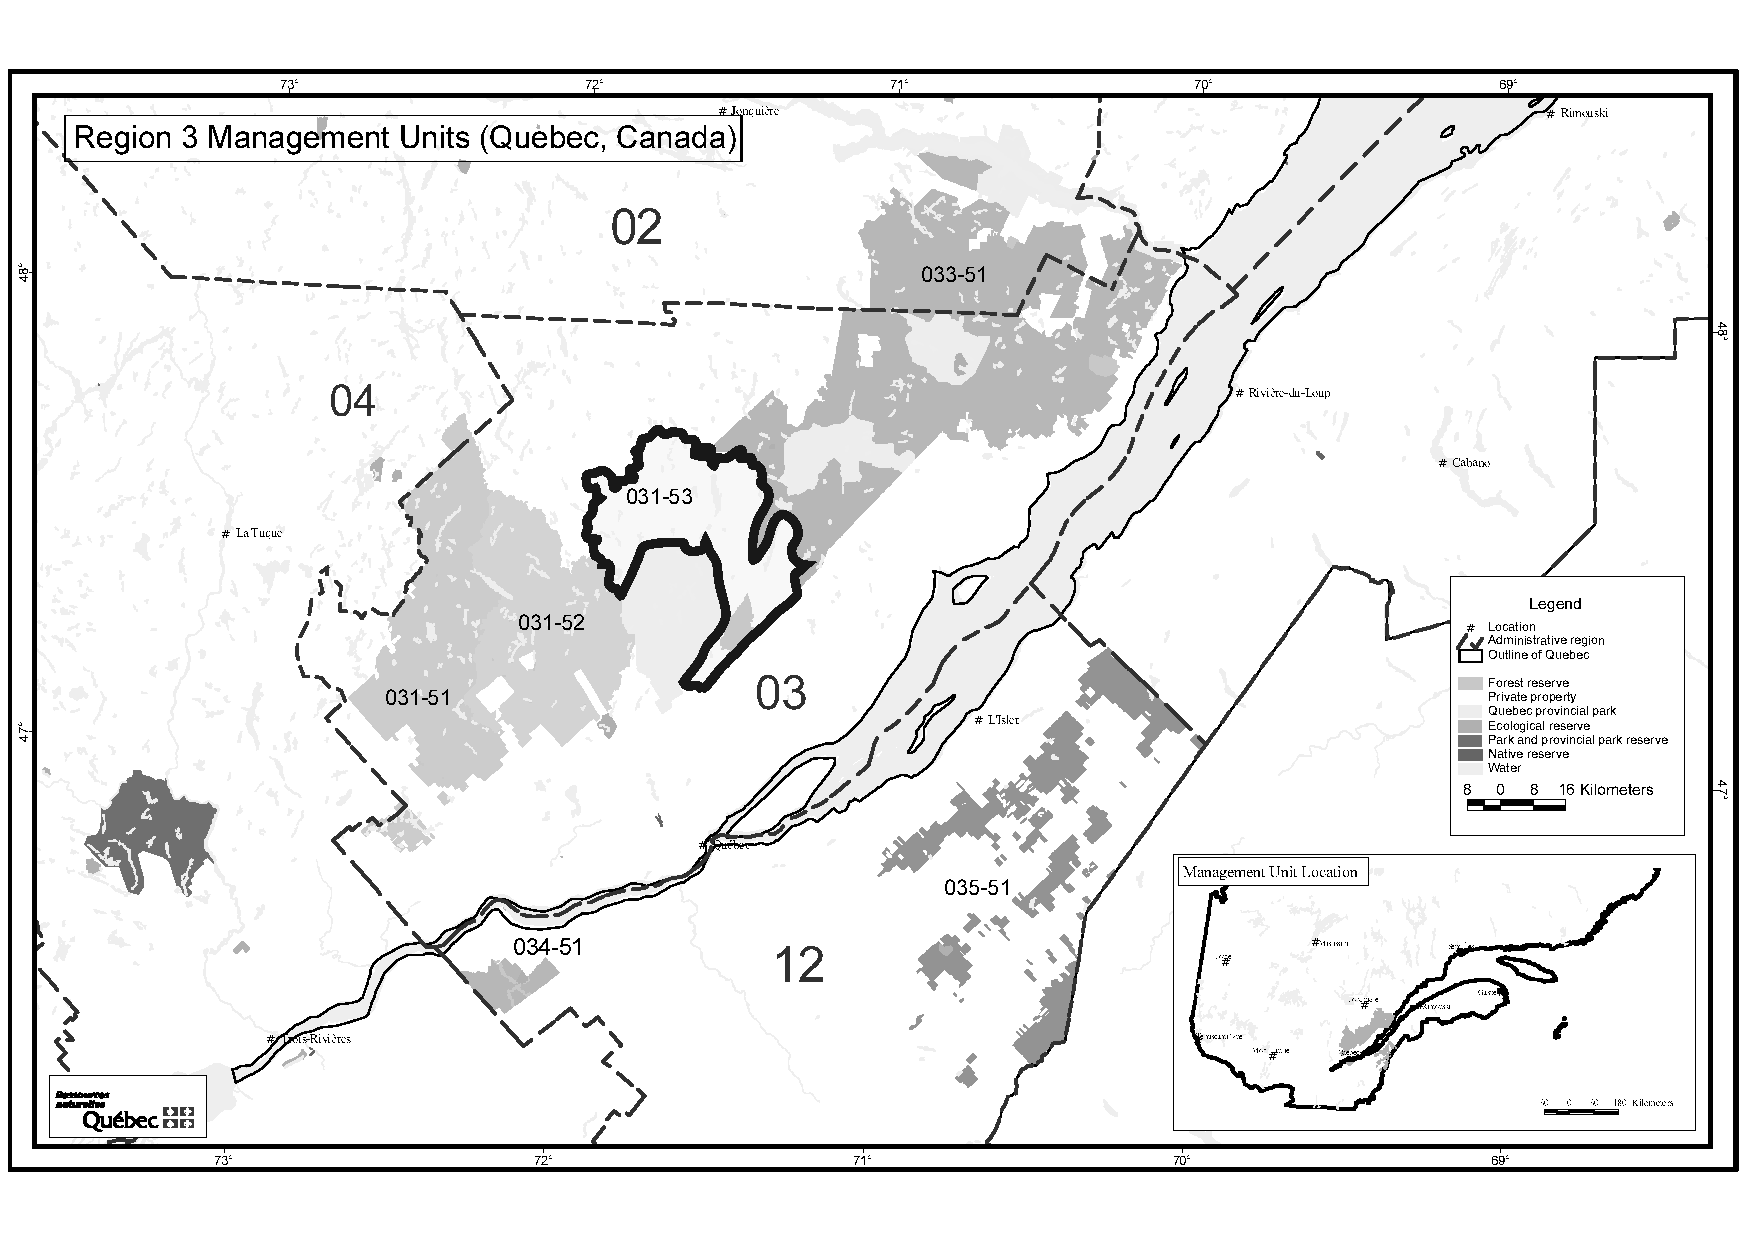
\includegraphics[width=\textwidth]{images/region-03_highlight}
\end{figure*}
 

Initial forest inventory, silviculture treatment eligibility and
operability, yield curves, and state transition matrix were all
compiled by government wood supply analysts for the 2013--2018 AAC
planning period. The test area is in the boreal forest region. The majority
(88\%) of initial growing stock is softwood%
\footnote{Mostly black spruce (\emph{Picea mariana}) and balsam fir
  (\emph{Abies balsamea}).%
}, with presence (12\%) of hardwood species%
\footnote{Mostly white birch (\emph{Betula papyrifera}) and poplar
  (\emph{Populus tremuloides}).%
}. Some pure softwood stands occur naturally, and plantations are
generally pure spruce. A significant proportion of the forest cover is
made up of mixed-wood stands containing different proportions of
hardwood mixed in with the softwood. Total productive area in this
management unit is 102 040 hectares. The most recently published official
AAC (determined by government planners) is 100 600 $m^{3}$ for
softwood and 9600 $m^{3}$ for hardwood.

We simulate one harvesting treatment (clearcut) and two silviculture
treatments (planting, pre-commercial thinning). No species-wise
selective cutting is possible (ie. hardwood must be harvested if
present) in mixed-wood stands.


\subsection{Value Creation Network Dataset}

For the short-term planning model, we compiled an illustrative case
study using realistic parameters (production capacities, unit cost of
raw logs, transformation process input/output maps, unit prices of
finished products). Parameter values used were originally collected
from industry partners in the course of previous research
projects. Figure \ref{fig:schematic-vcn} provides a schematic
representation of our value creation network test dataset,
illustrating potential product flow paths through the network. Note
that the entire value creation network is encapsulated within the
short-term planning agent.

\begin{figure}[ht!]
\caption{Schematic representation of test value creation network dataset}
\label{fig:schematic-vcn}
\centering{}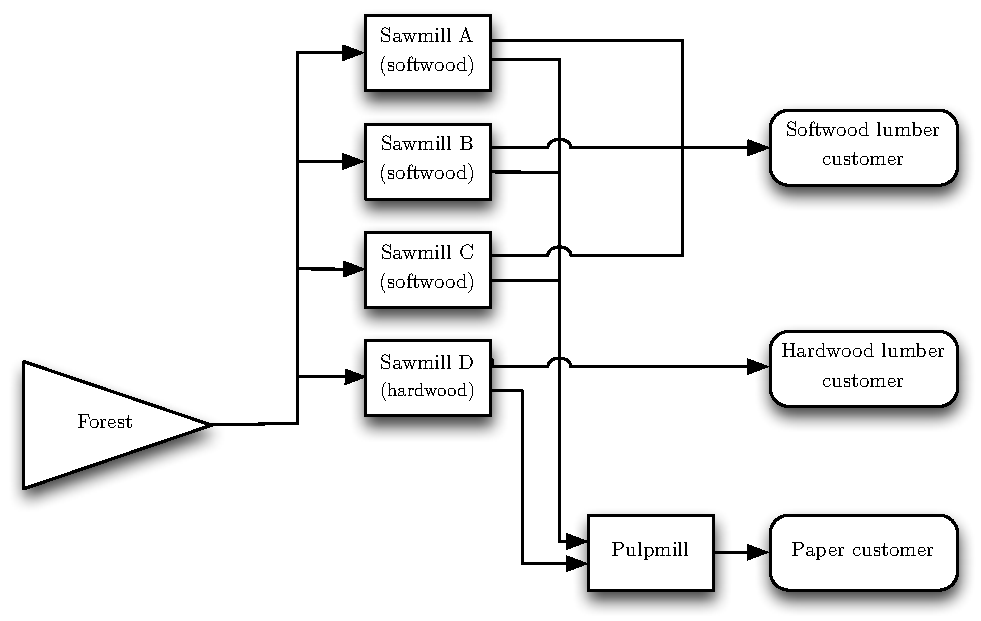
\includegraphics[width=\columnwidth]{images/vcn-schematic}
\end{figure}



\section{Experimental Design}
\label{sec:experiment}

Using our illustrative case study dataset, we tested for existence of
a SDE by simulating the \emph{status quo} hierarchical planning
process. We compared the output from our optimization model to the
original government wood supply model, and confirmed that our model
perfectly replicates source model structure (ie. initial inventory,
forest growth curves, treatment eligibility, state transitions
following treatment). Setting aside our simplification of objective
function and constraint structure, our model perfectly replicates a
\emph{status quo} long-term wood supply model, and thus provides a
reasonable basis for our illustrative case study.

% Original government-regulation--compliant AAC model includes a large
% number of constraints (many of which are non-binding and redundant)
% describing minimum greened-up area by watershed, constraints on
% minimum and maximum plantation and PCT treatment areas, constraints
% attempting to indirectly model cumulative effect of spatial harvest
% block layout regulations, and constraints limiting disturbance
% intensity around visually sensitive areas. We have not retained these
% constraints for our illustrative case study, in an effort to capture
% the essence of \emph{status quo} wood supply models using the simplest
% possible model formulation. We expect our simplified model to more
% clearly illustrates the systematic drift effect (SDE), and evacuation
% of complex Quebec-specific regulatory constraints will make it easier
% for practitioners in other jurisdictions to relate to our illustrative
% case study.

We defined six simulation scenarios, which vary in terms of demand
types, demand levels, and integration of long- and short-term planning
models. Table \ref{tab:scenarios} summarizes scenario parameters used
in the experiment. Each simulation is actually made up of 30 two-phase
(long-term, short-term) rolling-horizon re-planning iterations. All
scenarios maximize sum of even-flow softwood and even-flow hardwood
volume. The six scenarios can be grouped into three scenario-pairs,
which we describe below.

 % \footnote{Long-term optimization problem formulation similar to
 %  status quo definition of AAC in Quebec for wood supply planning on
 %  public land.}

Scenarios 1.1 and 1.2 maximize AAC independently of demand (ie. long-
and short-term plans not integrated, short-term model formulation
S1). Demand for short-term planning is assumed to be infinite
(ie. 100\% of AAC is harvested at each iteration). Scenario 1.1
simulates perfect implementation of period-1 solution at each
iteration (decision variable values preserved). In contrast, scenario
1.2 simulates \emph{imperfect implementation} of period-1 solution at
each iteration; first-period decision variables are re-optimized using
model formulation S1, subject to constraints forcing species-wise harvest
volume and silviculture treatment area to match first-period solution of the
long-term model solution. As noted previously in
\S\ref{sec:formulation-s1}, the short-term model will not
necessarily schedule the same first-period forest units (ie. strata)
as the long-term model. Thus implicit spatial distributions of long-
and short-term harvesting solutions may differ, both at
local (ie. harvest block) and landscape-level scales (considering
ecologically-driven spatial clustering of forest unit types on the
landscape).

Similarly to the previously described scenario-pair, scenarios 2.1 and
2.2 maximize AAC independently of demand (ie. long- and short-term
plans not integrated, short-term model formulation S1). Demand for
short-term model is intentionally set to an unbalanced subset of AAC
(80\% of softwood AAC, 40\% of hardwood AAC), which is similar to
historical harvest-to-AAC ratio observed in Quebec and other Canadian
provinces (see Table \ref{tab:harvestcontrol}). Scenarios 2.1 and 2.2
differ only in demand type. Scenario 2.1 assumes constant demand
(ie. demand level fixed for all rolling-horizon re-planning
iterations), whereas scenario 2.2 assumes proportional demand
(ie. demand level updated at each rolling-horizon re-planning
iteration to equal 80\% of softwood AAC and 40\% of hardwood AAC).

Scenarios 3.1 and 3.2 use the integrated model formulation (short-term
model formulation S2), which finds the long-term sustainable wood
supply solution that maximizes first-period profit of the value
creation network. As model formulation S2 maximizes profit over a
single planning period, we do not discount profit values as this would
have no impact on optimization model decisions. Scenario 3.1 is the
base scenario for this series. Scenario 3.2 adds an upper-bound
constraint on hardwood output from the long-term model. The value of this
constraint parameter is selected to match the hardwood processing capacity
in the value creation network (ie. a simple anticipation mechanism to
demonstrate potential benefits of improved linkages on hierarchical
planning process performance).

\begin{table}
\caption{Scenario descriptions}
\label{tab:scenarios1}
\renewcommand{\tabcolsep}{2pt}
\begin{tabular}{llll}
\toprule 
Scenario Name & Demand type & Demand level\tabularnewline
\midrule
1.1 & Infinite & 100\% of AAC (exact implementation of first-period solution)\tabularnewline
1.2 & Infinite & 100\% of AAC (re-optimized with short-term model)\tabularnewline
2.1 & Constant & 80\% of initial softwood AAC, 40\% of initial hardwood AAC\tabularnewline
2.2 & Proportional & 80\% of initial softwood AAC, 40\% of initial hardwood AAC\tabularnewline
3.1 & Constant & Integrated model (basic)\tabularnewline
3.2 & Constant & Integrated model (with long-term hardwood supply constraint) \tabularnewline
\bottomrule
\end{tabular}
\end{table}


\section{Results and Discussion}
\label{sec:results1}

Figures \ref{fig:scenario1.1} to \ref{fig:scenario3.2} present
simulation results for six scenarios. % Table \ref{tab:scenarios}
% summarizes scenario parameters used in the experiment for each
% scenario.
Disposition of figures is identical for all scenarios. The
first subfigure (a) for each scenario shows the initial
(ie. iteration-0) AAC solution. The second subfigure (b) for each
scenario shows first period of AAC solution for all 30 planning
iterations. The third subfigure (c) for each scenario shows the
implemented harvest level for all 30 planning iterations. Scenarios
3.1 and 3.2 also show profit in this subfigure on a secondary
axis. The fourth subfigure (d) for each scenario shows the difference
between initial and re-planned AAC. The fifth subfigure (e) for each
scenario shows the difference between re-planned AAC and harvest.  The
sixth subfigure (f) for each scenario shows the difference between
initial AAC and harvest. Softwood volume is shown with white bars,
hardwood volume with black bars, and total volume with small
circles. Profit (where applicable) is shown with the $\times$
symbol. 

Table \ref{tab:compare_volume-profit} compares harvested volume and
profit for the first seven planning iterations, for scenarios 3.1 and
3.2. We do not include the first two scenario-pairs here, as only the
third scenario-pair uses integrated short-term model formulation S1,
which allows us to compare profit and harvest volume.

Note that profit values presented here are not discounted, as
short-term planning model formulation S2 maximizes profit over a
single 5-year planning period. Although it would be possible to apply
an arbitrary discount rate \emph{a posteriori} to profit values in
Table \ref{tab:compare_volume-profit}, this would have no impact on
iterative simulation solutions. Our long-term model formulation does
not include any profit performance indicators.

Although we simulated a large number of scenarios, we retained only
three scenario-pairs for illustrative purposes. The first
scenario-pair (1.1 and 1.2) is presented as a base case, to show
relative stability of long-term solution when actual harvest at each
planning cycle closely (or perfectly) matches AAC solution. The second
scenario-pair shows instability of long-term wood supply when timber
demand is a skewed subset of wood supply, and simulates the
possibility of wood supply failures under these conditions. The third
scenario-pair shows potential benefit (on stability of wood
supply and value-creation potential) of integrating a simple
demand-anticipation mechanism into the long-term planning process.

% Scenario 1.1  %
\begin{figure}[ht!]
  \caption{Scenario 1.1: (a) initial optimal solution, (b) iterative
    as-planned solution, (c) iterative as-implemented solution, (d)
    difference between iterative as-planned and initial solutions, (e)
    difference between iterative as-implemented and iterative
    as-planned solutions, (f) difference between iterative
    as-implemented and initial solutions. Softwood volume is shown
    with white bars, hardwood volume with black bars, and total volume
    with small circles.}
  \label{fig:scenario1.1}
  \medskip
  \centering
  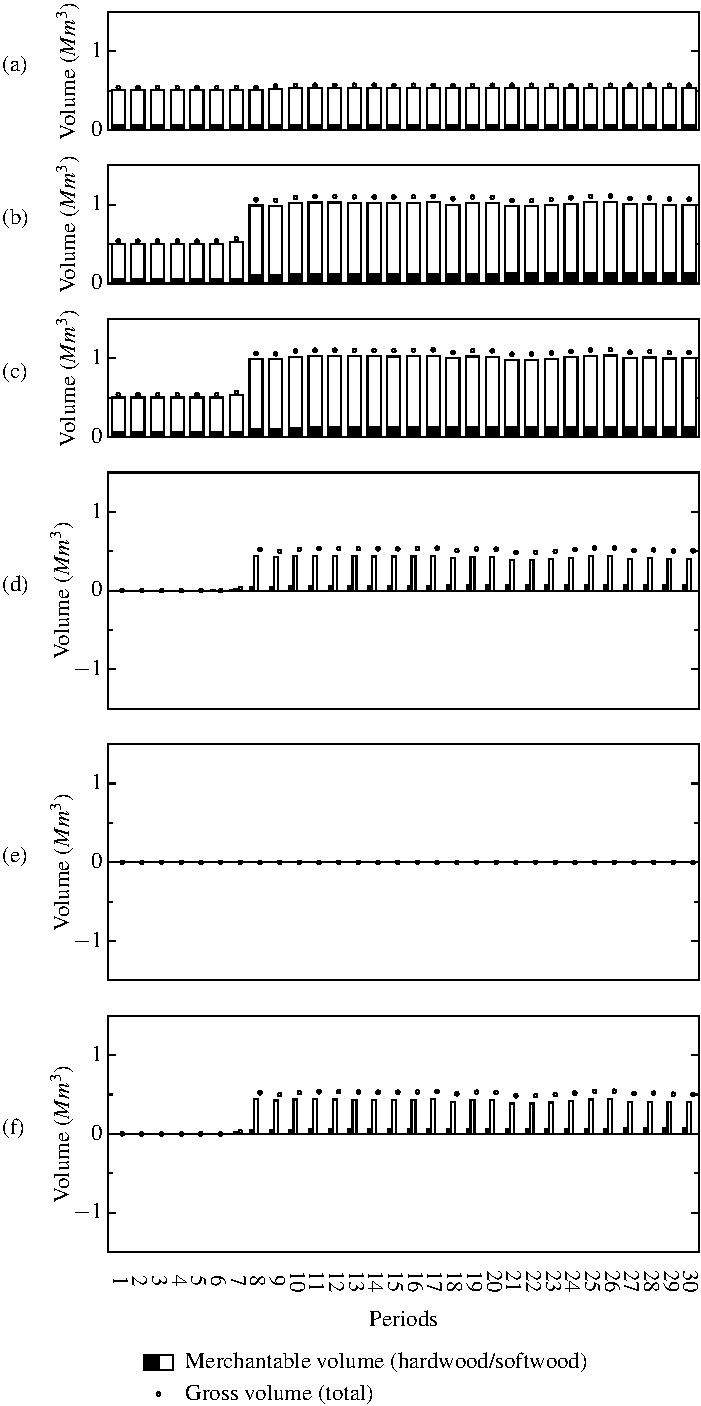
\includegraphics[width=0.6\columnwidth]{images/s2-1a}
\end{figure}

% Scenario 1.2 %
\begin{figure}[ht!]
  \caption{Scenario 1.2: (a) initial optimal solution, (b) iterative
    as-planned solution, (c) iterative as-implemented solution, (d)
    difference between iterative as-planned and initial solutions, (e)
    difference between iterative as-implemented and iterative
    as-planned solutions, (f) difference between iterative
    as-implemented and initial solutions. Softwood volume is shown
    with white bars, hardwood volume with black bars, and total volume
    with small circles.}
  \label{fig:scenario1.2}
  \medskip
  \centering
  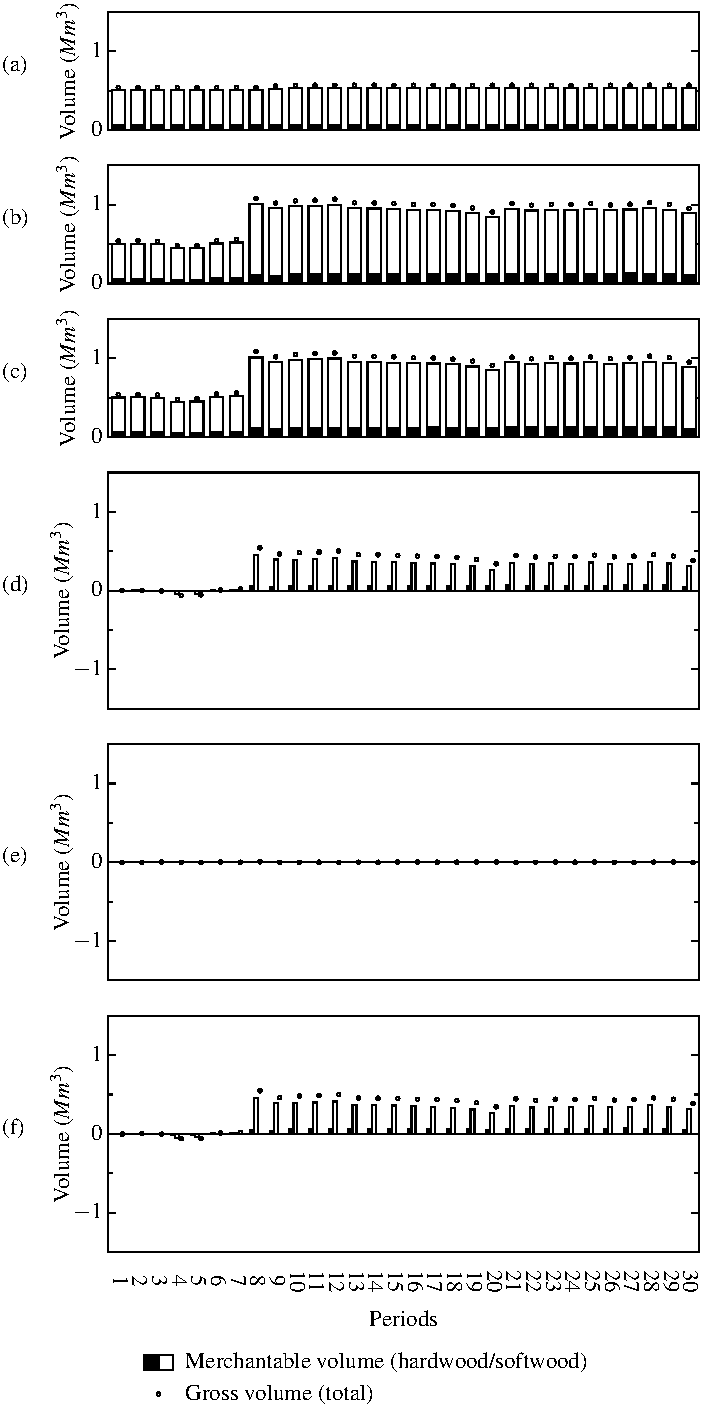
\includegraphics[width=0.60\columnwidth]{images/s2-1b}
\end{figure}

% Scenario 2.1 %
\begin{figure}[ht!]
  \caption{Scenario 2.1: (a) initial optimal solution, (b) iterative
    as-planned solution, (c) iterative as-implemented solution, (d)
    difference between iterative as-planned and initial solutions, (e)
    difference between iterative as-implemented and iterative
    as-planned solutions, (f) difference between iterative
    as-implemented and initial solutions. Softwood volume is shown
    with white bars, hardwood volume with black bars, and total volume
    with small circles.}
  \label{fig:scenario2.1}
  \medskip
  \centering
  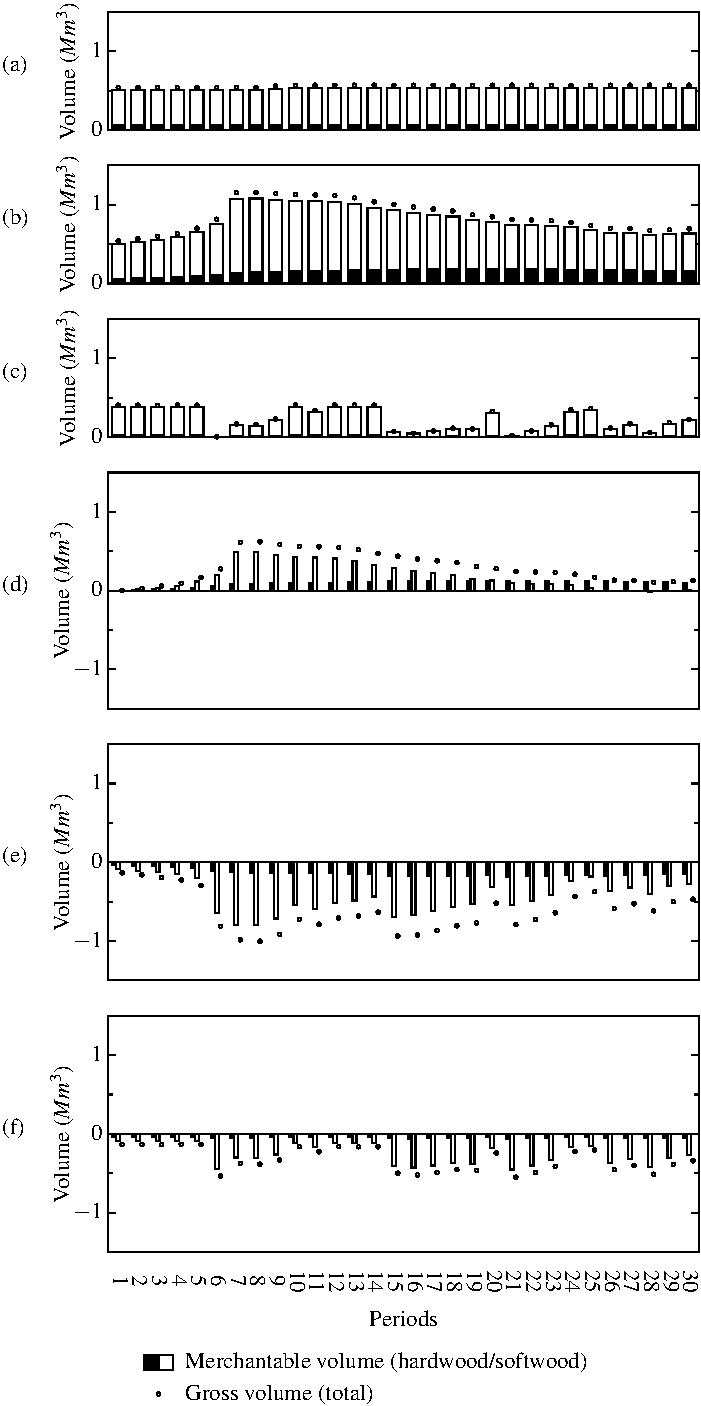
\includegraphics[width=0.60\columnwidth]{images/s2-2c}
\end{figure}

% Scenario 2.2 %
\begin{figure}[ht!]
  \caption{Scenario 2.2: (a) initial optimal solution, (b) iterative
    as-planned solution, (c) iterative as-implemented solution, (d)
    difference between iterative as-planned and initial solutions, (e)
    difference between iterative as-implemented and iterative
    as-planned solutions, (f) difference between iterative
    as-implemented and initial solutions. Softwood volume is shown
    with white bars, hardwood volume with black bars, and total volume
    with small circles.}
  \label{fig:scenario2.2}
  \medskip
  \centering
  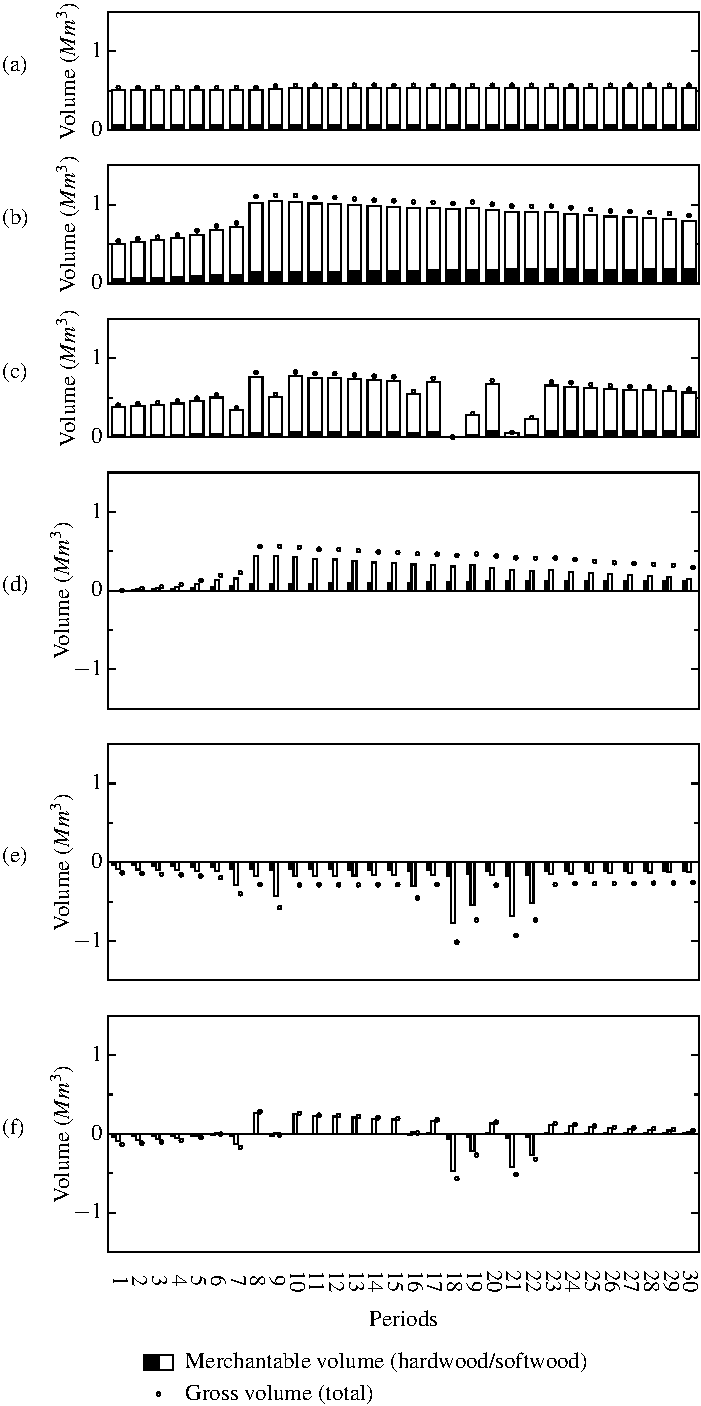
\includegraphics[width=0.60\columnwidth]{images/s2-3b}
\end{figure}

% Scenario 3.1 %
\begin{figure}[ht!]
  \caption{Scenario 3.1: (a) initial optimal solution, (b) iterative
    as-planned solution, (c) iterative as-implemented solution, (d)
    difference between iterative as-planned and initial solutions, (e)
    difference between iterative as-implemented and iterative
    as-planned solutions, (f) difference between iterative
    as-implemented and initial solutions. Softwood volume is shown
    with white bars, hardwood volume with black bars, and total volume
    with small circles. Profit is shown with the
    $\times$ symbol.}
  \label{fig:scenario3.1}
  \medskip
  \centering
  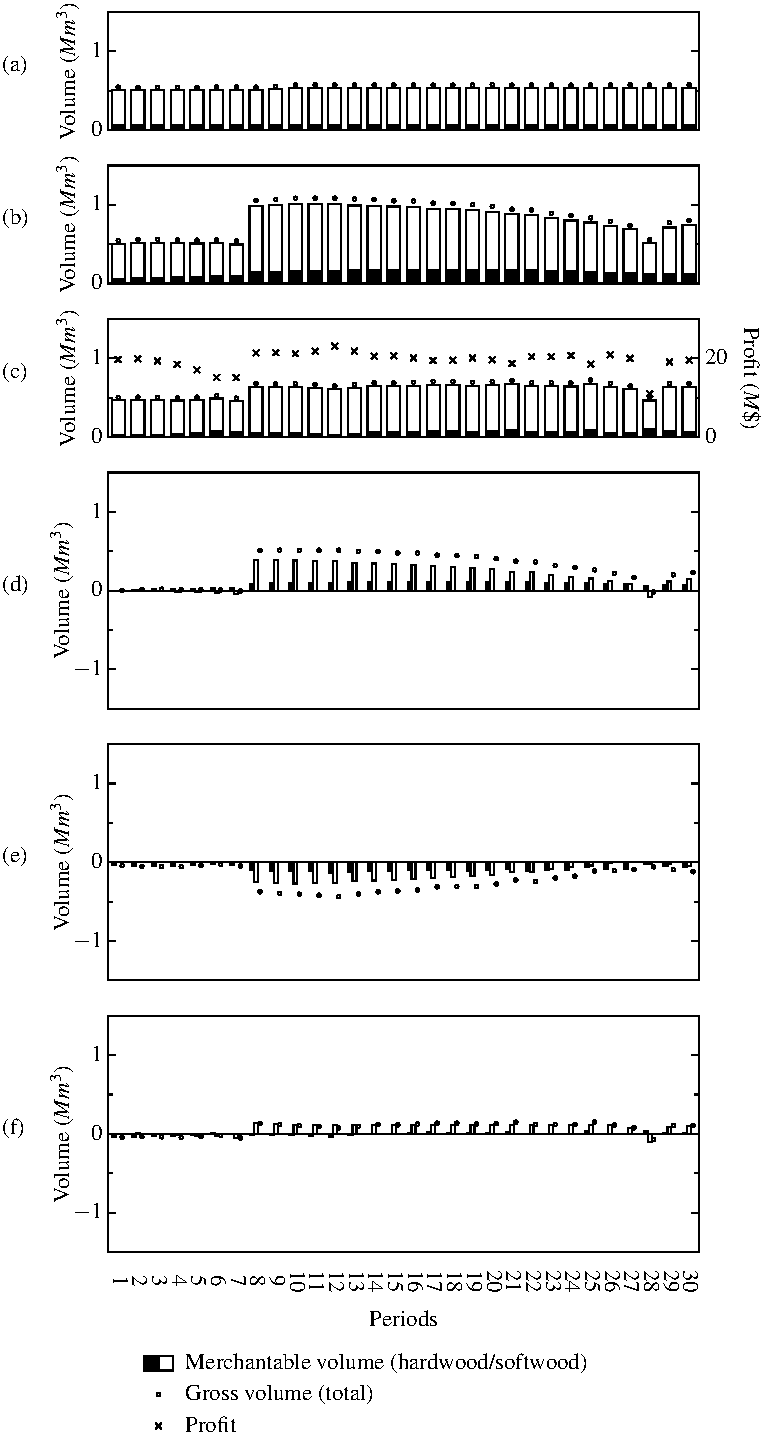
\includegraphics[width=0.65\columnwidth]{images/s3-1}
\end{figure}

% Scenario 3.2 %
\begin{figure}[ht!]
  \caption{Scenario 3.2: (a) initial optimal solution, (b) iterative
    as-planned solution, (c) iterative as-implemented solution, (d)
    difference between iterative as-planned and initial solutions, (e)
    difference between iterative as-implemented and iterative
    as-planned solutions, (f) difference between iterative
    as-implemented and initial solutions. Softwood volume is shown
    with white bars, hardwood volume with black bars, and total volume
    with small circles. Profit is shown with the
    $\times$ symbol.}
  \label{fig:scenario3.2}
  \medskip
  \centering
  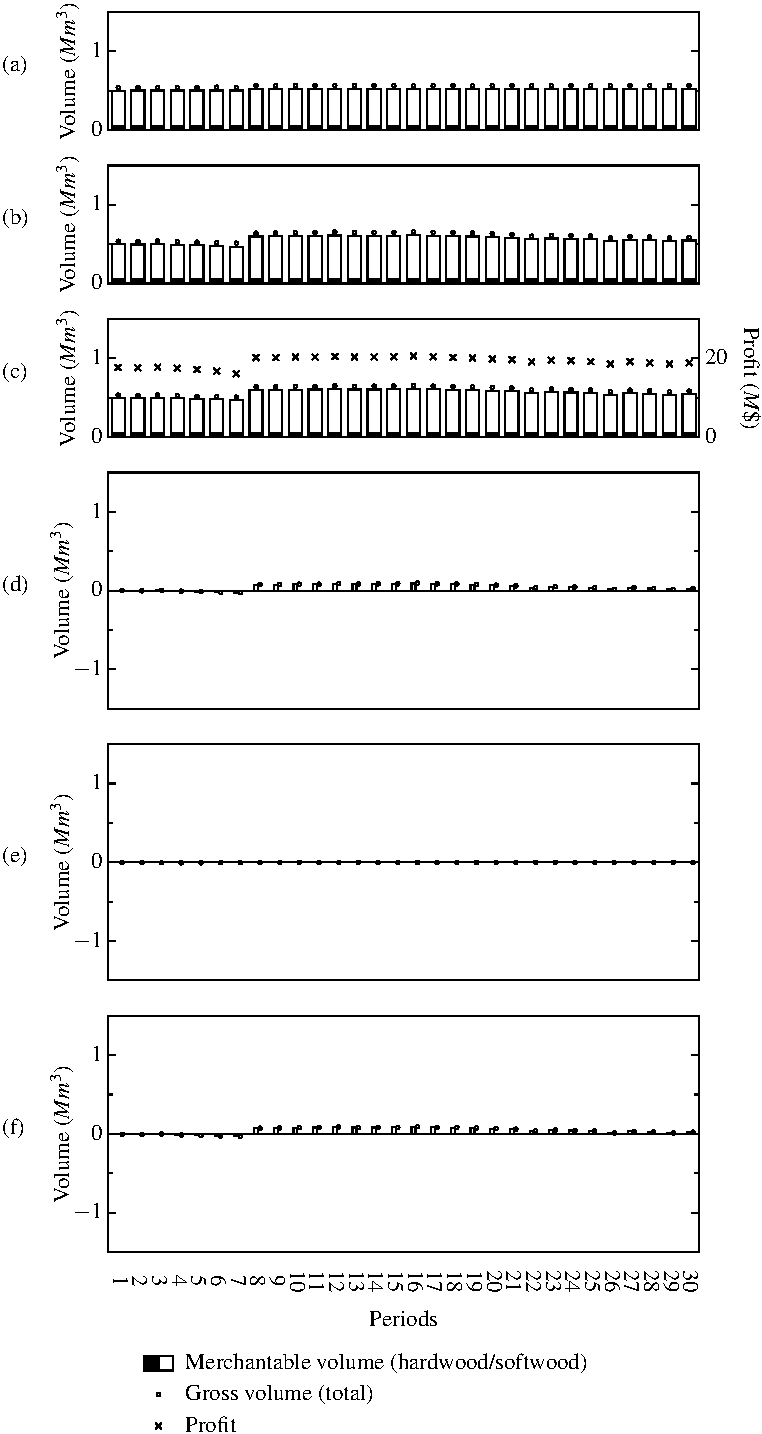
\includegraphics[width=0.65\columnwidth]{images/s3-2}
\end{figure}

\begin{table}[ht!]
\caption{Comparison of harvested volume and profit for periods 1--7 (scenarios 3.1 and 3.2)}
\label{tab:compare_volume-profit}
\renewcommand{\tabcolsep}{11pt}
\begin{tabular}{lrrrrrr}
\toprule
 & \multicolumn{2}{c}{Scenario 3.1} & \multicolumn{2}{c}{Scenario 3.2} & \multicolumn{2}{c}{Difference}\tabularnewline
Iteration & Volume & Profit & Volume & Profit & Volume & Profit\tabularnewline
 & (thousand $m^3$) & ($M\$$) & (thousand $m^3$) & ($M\$$) & ($\%$) & ($\%$)\tabularnewline
\midrule 
1 & 501 & 19.7 & 533 & 17.7 & 6 & -10\tabularnewline
2 & 507 & 19.9 & 530 & 17.6 & 5 & -11\tabularnewline
3 & 505 & 19.3 & 535 & 17.7 & 6 & -8\tabularnewline
4 & 496 & 18.5 & 525 & 17.5 & 6 & -5\tabularnewline
5 & 507 & 17.1 & 518 & 17.1 & 2 & 1\tabularnewline
6 & 527 & 15.1 & 516 & 16.7 & -2 & 11\tabularnewline
7 & 494 & 15.1 & 507 & 16.1 & 3 & 6\tabularnewline
\midrule 
Mean & 505  & 17.8 & 523 & 17.4 & 4 & -3 \tabularnewline
CV & 2 & 11 & 2 & 3 & 0 & -7 \tabularnewline
\bottomrule
\end{tabular}
\end{table}

% \section{Discussion}
% \label{sec:discussion}


As can be expected for scenario 1.1 (perfect implementation of
period-1 solution at each iteration), re-planned AAC solutions track
perfectly along initial optimal solution until a critical period is reached
(ie. period 7), after which AAC increases sharply and remains relatively
stable despite re-planning at each period, indicating negligible
influence of end-of-horizon effects on simulation results and low
systematic drift effect (SDE). The situation is noticeably different
for scenario 1.2 (imperfect implementation of first-period optimal
solution): AAC steadily declines until critical period, then increases sharply
after the critical period as new growing stock becomes available, and
resumes steady decline (see Figure \ref{fig:scenario1.2}(b)). This
\emph{declining non-declining yield} phenomenon is discussed in the
literature
\citep{mcquillan1986declining,daugherty1991credibility,gunn2007models},
however little has been done to address this issue in practice. Note
that documented cases of \emph{declining non-declining yield} in the
literature are all based on models with profit maximization objectives
(with even-flow constraints), whereas our model uses a volume
maximization objective (with even-flow constraints).

Scenarios 1.1 and 1.2 demonstrate that \emph{status quo} implementation of
the AAC model, if used within a \emph{status quo} rolling-horizon
hierarchical planning context, does not guarantee non-declining future
harvest levels \emph{even if the first period of optimal solution is
  implemented almost perfectly} and deterministic model assumptions
are assumed to hold. Undesirable behaviour of the AAC model under
these optimistic base-case conditions (ie. high level of coherence
between long- and short-term plans) shows that the \emph{status quo} planning
process is sensitive to even the smallest deviations from the
long-term optimal solution during its implementation. The infinite
demand assumption behind these first two scenarios is unrepresentative
of the \emph{status quo} planning context in many jurisdictions; harvest volumes
are generally well below AAC, and choice of harvest blocks may
include significant biases relative to optimal AAC solution
(ie. closest to access roads, least dispersed, etc).

Scenarios 2.1 and 2.2 simulate impact of incoherence between supply
and demand assumptions in planning models. For both scenarios,
species-wise demand distribution is a skewed subset of supply. We
project current demand forward in two different ways. Scenario 2.1
assumes constant demand pattern (ie. species-wise demand is not updated
at each rolling-horizon re-planning iteration). Scenario 2.2 assumes
proportional demand (ie. species-wise demand is updated at each
rolling-horizon re-planning iteration, always using 80\% and 40\% of
most recently calculated softwood and hardwood AAC). Scenario 2.1
simulates an unsustainable trajectory; Figure \ref{fig:scenario2.1}(c)
shows a wood supply failure in period 6, followed by regular wood
supply failures later in the planning horizon. These wood supply
failures are induced by systematic omission of hardwood-rich forest
units from short-term harvest plans, and are not predicted by the
long-term wood supply model. In fact, the long-term wood supply model
had been predicting \emph{increasing} AAC levels\footnote{Increasing
  AAC can be explained by unanticipated accumulation of growing stock
  in the forest, due to harvest levels systematically below AAC.} for
several rolling-horizon planning iterations when the first wood supply
failure occurs (see Figure \ref{fig:scenario2.1}(b)). Scenario 2.2
simulates less severe wood supply failures, in part because we allow
species-wise demand to scale up and down (as a proportion of current
AAC) at each rolling-horizon re-planning iteration, thereby ensuring
a certain adaptive coherence between supply and demand (despite
a systematic species-skewed gap between planned and implemented harvest levels).

Scenarios 3.1 and 3.2 demonstrate some potential advantages of
integrating long- and short-term planning. In our integrated model,
the long-term wood supply plan is driven by short-term value creation,
\emph{viz.} the  wood supply solution is iteratively adjusted until it
converges on an even-flow wood supply plan that maximizes first-period
profit. Note that process parameters have
been set in our model such that softwood processing is generally more
profitable than hardwood processing (consistent with current situation
in Quebec according to industry data). Scenario 3.1 shows a
significant decline in profits between periods 1 and 7 which we
explain by low hardwood demand relative to projected hardwood harvest
levels in the long-term wood supply plan: at every iteration, the short-term planning agent
systematically avoids harvesting (less profitable) hardwood-rich
stands. Lower-value hardwood growing stock accumulates, causing
a systematic decline of value-creation potential in the medium term;
this scenario is clearly not sustainable.

We added a simple constraint to the wood supply model in Scenario 3.2,
which sets an upper bound on long-term hardwood harvest projection
to (approximately) match hardwood demand in the value creation
network. The impact of improved coherence between long- and short-term
planning processes is obvious: optimizing long-term hardwood supply
planning to more closely match long-term demand eliminates much of the
softwood high-grading behaviour observed in scenario 3.1,
resulting in stabilized profit and volume flow, and increased mean AAC
for the first seven planning iterations (see Figures
\ref{fig:scenario3.1}(c) and \ref{fig:scenario3.2}(c), and Table
\ref{tab:compare_volume-profit}).

The last five scenarios all exhibit some form of \emph{systematic
  drift effect} (SDE) that is not predicted by the long-term wood
supply optimization model. Evidence of SDE in our illustrative case
study includes a monotonic increase or decrease in AAC over several
iterations, a monotonic change in AAC composition (ie.  ratio of
hardwood to softwood), increasing incoherence between supply and
demand, and increasing infeasibility of the demand-satisfaction problem
(ie. instability of simulated harvest levels). Undetected forms of
drift are likely to exist within these scenarios for performance
indicators not presented here (eg. standing timber inventory, age
class distribution, landscape patch distribution, value-creation
potential, harvest block size and location distribution, wildlife
habitat suitability, etc).


\section{Conclusion}
\label{sec:conclusion1}

The illustrative case study presented here shows that the \emph{status quo}
hierarchical forest planning process (ie. two-phase rolling-horizon
iterative re-planning) is incoherent and dysfunctional: it fails to
demonstrate long-term sustainability of government-endorsed short-term
harvest levels, fails to reliably meet industrial fiber demand over
time, and exacerbates incoherence between wood supply and fiber demand
over several planning iterations. We identify systematic differences
between planned and actual harvesting activities as an important
factor contributing to this dysfunction, which manifests itself as
either instability in long-term wood supply or lost short-term value
creation opportunity.

We show that coherence between long- and short-term planning solutions
can be improved significantly by manipulating linkages between
planning levels (eg. adding species-wise demand constraint to the AAC
model). Although simplistic in its implementation, our integrated
model illustrates the potential value (in terms of both credibility of
long term planning process and performance of short-term planning
process) of anticipating short-term planning objectives (eg. demand
satisfaction) within a long-term planning model. Based on our
preliminary simulation results, we feel there is much potential for
further refinement of linkages between long- and short-term planning processes.

Much of the difference between planned and actual harvesting activities
can be explained by the principal-agent relationship between
government and industry planners. This principal-agent relationship
could potentially be modelled as a bi-level optimization problem, and
the long-term planning process extended to include an
anticipative-iterative dimension. This would allow the principal to
develop long-term forest policy that is more likely to be compatible
with anticipated agent behaviour, thereby inducing a reduction in SDE, and
improving hierarchical planning process credibility and value-creation potential.

% We propose changes to the long-term planning process that
% may produce more effective contracts, thus reducing the gap between
% projected and actual agent behaviour, thereby improving credibility of
% government policy as a tool for ensuring long-term sustainability of
% forest resources. Furthermore, more efficiently designed contract
% between principal and agent may reduce pressure on constraints and
% incentives required to achieve desired outcome from the planning
% process, thereby providing a more flexible and agile short-term
% planning environment for the agent. In other words, an optimal design
% for the hierarchical forest management process ensures long-term
% sustainability of the forest resource while providing maximum
% short-term value-creation opportunity for the forest industry.

\section{Acknowledgements}

This study was supported by funding from the \emph{FORAC Research
  Consortium} and the \emph{Fonds de recherche du Qu\'{e}bec -- Nature
  et technologies}. The authors would like to thank
Dr. Fr\'{e}d\'{e}ric Raulier and the two anonymous reviewers for their
valuable comments and suggestions during the writing process, which
greatly helped improve the quality of this paper.

\bibliographystyle{plainnat}
\bibliography{phd}


%%% Local Variables: 
%%% mode: latex
%%% TeX-master: "909303058"
%%% End: 
\setcounter{secnumdepth}{3} 

%\chapter{Extenting the Classic Woods Supply Model to Anticipate Industrial Fibre Consumption}
\chapter{A Bilevel Model Formulation for the Distributed Wood Supply Problem}

This chapter presents an article entitled \emph{A Bilevel Model Formulation for the Long-Term Wood Supply Problem}, submitted to the \emph{European Journal of Operational Research}. The authours are Gregory Paradis, Mathieu Bouchard, Luc LeBel, and Sophie D'Amours.

\pagebreak

\selectlanguage{francais}

\begin{abstract}
  French abstract goes here.
\end{abstract}

%\pagebreak

\selectlanguage{english}

\begin{abstract}
    The classic wood supply optimization model maximizes sustainable (i.e., even-flow) harvest levels, and implicitly assumes infinite fibre demand.
  In many jurisdictions, this modelling assumption is a poor fit for actual fibre consumption, which is often a species-unbalanced subset of total fibre allocation. 
  Failure to anticipate this negative bias in volume and species mix of industrial wood fibre consumption has been linked to increased risk of future wood supply failure.
  In particular, we examine the \emph{distributed wood supply planning problem}, which is a variant of the the general wood supply planning problem where roles of forest owner and fibre consumer are played by independent agents (for example, wood supply planning on public forest land in Canada, where government stewards control wood supply and forest products industry firms consume the fibre).
  We use agency theory to describe the source of antagonism between public forest land owners (the \emph{principal}) and industrial fibre consumers (the \emph{agent}).
  We show that the distributed wood supply planning problem can be modelled more accurately using a bilevel formulation, and present an extension of the classic wood supply optimization model which explicitly anticipates industrial fibre consumption behaviour.
  The general case of the bilevel wood supply optimization problem is $\mathcal{NP}$-hard and non-convex; it is very difficult to solve to global optimality.   
  By imposing certain restrictions on the topology of the lower-level problem, we show that the problematic general case can be decomposed into convex sub-problems.
  We present a solution methodology that can solve this special case to global optimality, and compare output and solution times of classic and bilevel model formulations using a computational experiment on a realistic dataset.
  Computational results show that solution time for the decomposed bilevel problem is comparable to solution time for the classic single-level problem, and that the bilevel formulation can completely eliminate the problematic fibre consumption bias.
\end{abstract}

\pagebreak

\section{Introduction}
\label{sec:introduction2}

The concept of sustainable forest management (SFM) has long been a central theme of Crown (public) forest policy in Canada \citep{ccfm2008vision}. In concrete terms, sustainable forest management policy is implemented via silviculture treatments, notably harvesting treatments. According the the \emph{Criteria and Indicators of Sustainable Forest Management in Canada} \citep{ccfm2006criteria}, harvesting is generally deemed to be sustainable if it is below annual allowable cut (AAC) level. 

% In the case of forest management on public land, the relationship between government steward and industrial fibre consumer can be described as an instance of the \emph{principal-agent problem}.
% Government stewards (the principal) manage the land and grant timber harvesting licenses to industrial fibre consumers (the agent). The principal develops long-term forest management plans. Achievement of the principal's long-term goals depends requires that his plan be executed exactly. These plans are essentially composed of a sequence of harvesting treatment prescriptions, assuming a certain type, location, and timing for each treatments. The agent is typically responsible for planning and executing the short-term harvesting activities, which allow him to procure fibre for his mills. For a number of reasons, including logistical and economical factors, the agent will not willingly adhere exactly to the harvesting treatment sequence in the long-term plan. The antagonism in this principal-agent problem stems from the principal's dependency to implement the harvesting activities that constitute his long-term plan.

AAC is commonly determined using mathematical optimization models. 
The classic Model I \citep{davis2001forest-ch13} wood supply model formulation is the \emph{de-facto} standard wood supply planning tool in many jurisdictions.  
This classic model formulation finds the maximum indefinitely-sustainable\footnote{These models actually have a finite planning horizon. Typical rule-of-thumb horizon length choice would double the average timber rotation period. For example, a typical rotation period in the boreal forest is 75 years; a common wood supply model planning horizon is 150 years, discretized into 30 five-year periods. Planners assume that simulating sustainability over this horizon is sufficient to demonstrate indefinite sustainability.} harvest level, based on the implicit assumption that local fibre demand will always exceed supply.
In other words, the classic model assumes that all available fibre will be consumed in every planning period, regardless of quantity, quality, cost, or value creation potential.
In practice, this infinite-demand assumption is rarely respected.
Consequently, the classic wood supply optimization model tends to systematically over-estimate fibre consumption. Thus, we can expect that the principal's plan will never be executed, and that the long-term state of the forest may be quite different from that predicted by the classic wood supply model.

In this context, \citet{paradis2013risk} show that the classic model may fail when AAC exceeds industrial demand, and recommend further constraining the wood supply model based on anticipated fibre demand. This paper presents a novel bilevel extension of the classic formulation, which explicitly anticipates industrial fibre consumption using a subordinate optimization model to capture the agent's profit-maximization behaviour.
%We implement this recommendation using a bilevel model formulation.
Our bilevel model finds the maximal species-wise even-flow wood supply levels that we anticipate will be entirely consumed by a profit-maximizing industrial fibre consumer, thereby reducing the magnitude of the negative fibre consumption bias (relative to the classic wood supply model formulation).  
We show that the solution space induced by the bilevel reformulation is non-convex, which makes the general case difficult to solve exactly. 
We proceed to describe a special convex case of the problem that can be solved to global optimality using a decomposition-based solution methodology. 
%Finally, we test our solution methodology on a dataset of realistic size and complexity, to demonstrate algorithmic convergence and problem tractability.

The objectives of this study are to (a) compare the long-term performance of the classic and bilevel wood supply optimization model formulations after several rolling-horizon planning cycles, and (b) provide recommendations for improving the credibility of the wood supply planning process.

\section{Background}
\label{sec:background2}

The term \emph{wood supply planning} describes the process by which AAC is determined. In practice this typically amounts to solving a linear programming (LP) optimization model, which maximizes AAC subject to even-flow constraints \citep{gunn2007models}. Provincial government authorities allocate timber licences (TL) to industrial fibre consumers. These TLs set (species-wise) upper bounds on periodic harvest volume, however there is typically no policy requirement to set matching lower bounds. 

%This implies that 

%Wood supply planning plays an important role in sustainable forest management. This is particularly true on Crown (public) forest land in Canada, where government steward manage the forest resource on behalf of the Canadian people. 

Timber licences are typically valid for a pre-determined period (e.g., 5 years), after which point licenses may be renewed, subject to re-evaluation of species-wise AAC. Figures \ref{fig:aac} and \ref{fig:jointdist}(a) show species-wise Canadian AAC data from 1990 to 2012. Although there is some fluctuation over time, total national AAC has been relatively stable during this period.

For a variety of economic and logistic reasons, some portions of AAC are not attractive to timber licensees and are not harvested. Figures \ref{fig:aac_consumption} and \ref{fig:jointdist}(b) show species-wise proportion of Canadian AAC consumption from 1990 to 2012. On average, 80\% of softwood AAC is consumed, versus 45\% of hardwood AAC, indicating a clear industrial preference for softwood. Consumption rates for both species groups show similar variability. Softwood AAC consumption appears to be following a slight downward trend, whereas hardwood AAC consumption appears to be on the rise. 

\begin{figure}[h]
  \centering
  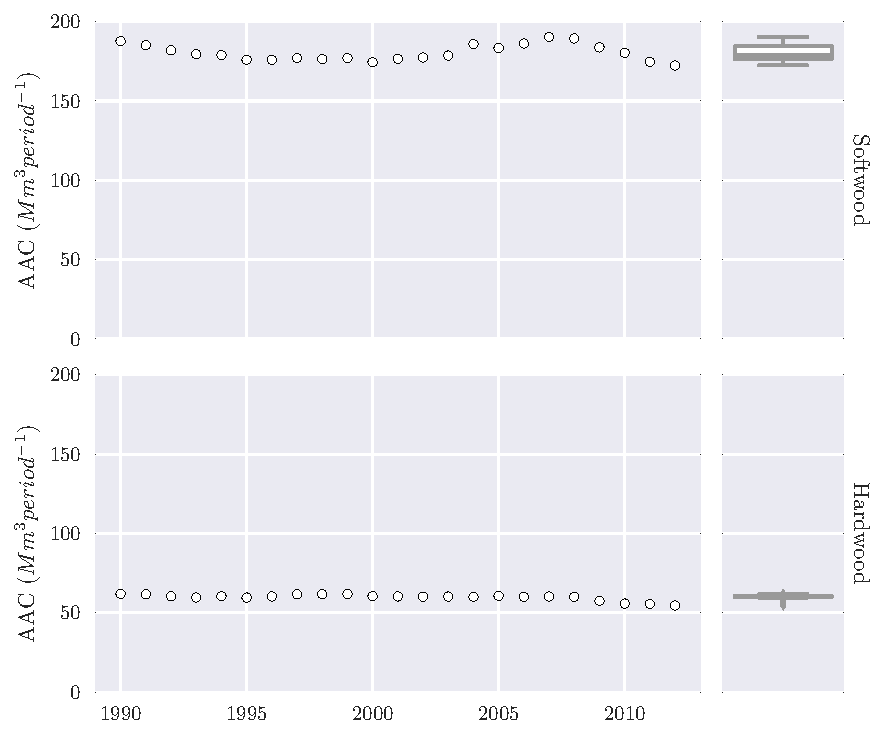
\includegraphics[width=\textwidth]{images/aac}
  \caption{Species-wise AAC consumption for period 1990 to 2012}
  \label{fig:aac}
\end{figure}

\begin{figure}[h]
  \centering
  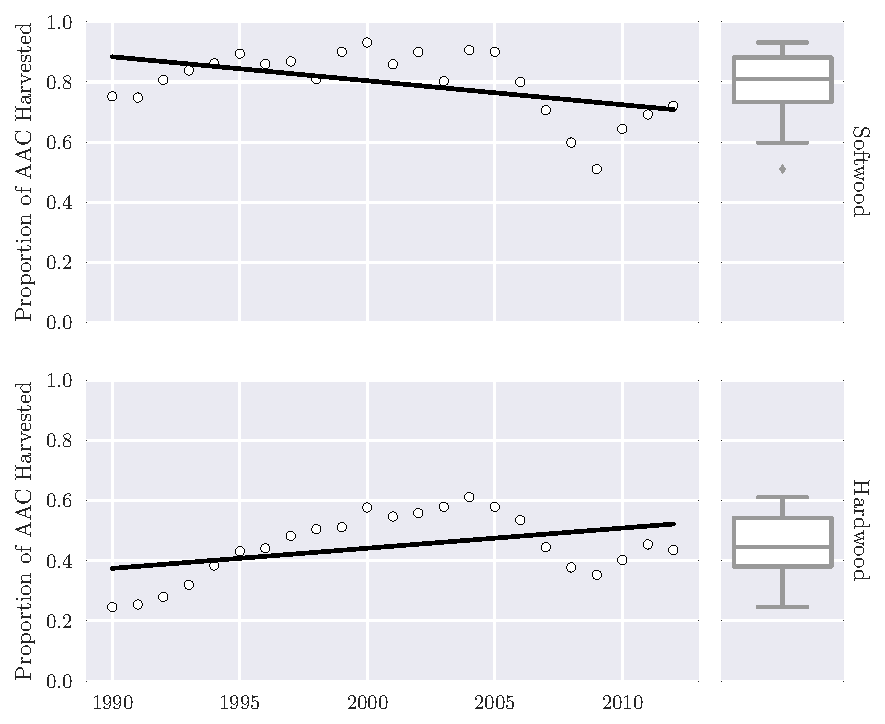
\includegraphics[width=\textwidth]{images/aac_consumption}
  \caption{Proportion of species-wise AAC consumed for period 1990 to 2012}
  \label{fig:aac_consumption}
\end{figure}

\begin{figure}[t]
    \centering
    \subfloat[AAC]{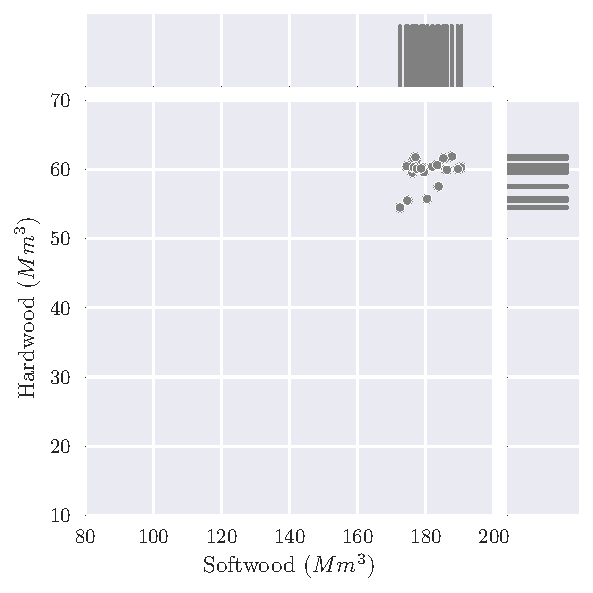
\includegraphics[width=0.5\textwidth]{images/aac_jointplot}}
    \subfloat[Fibre consumption]{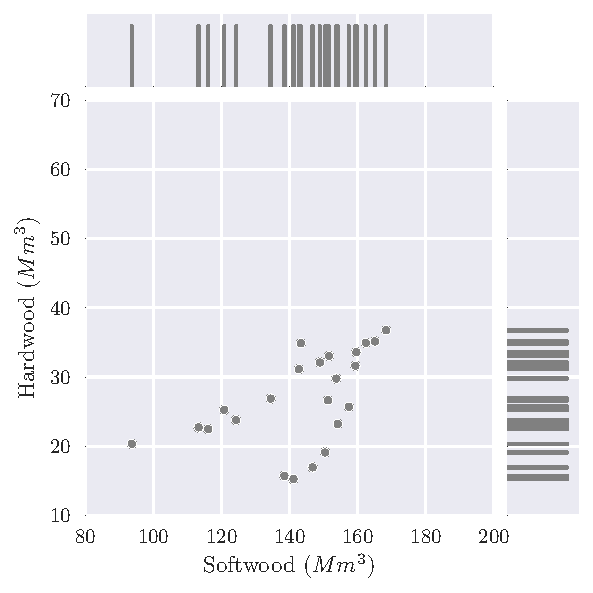
\includegraphics[width=0.5\textwidth]{images/harvest_jointplot}}
  \caption{Species-wise joint distributions of AAC and harvest volume for period 1990 to 2012}
  \label{fig:jointdist}
\end{figure}

% \begin{figure}[t]
%     \centering
%     \begin{subfigure}[t]{0.5\textwidth}
%         \centering
%         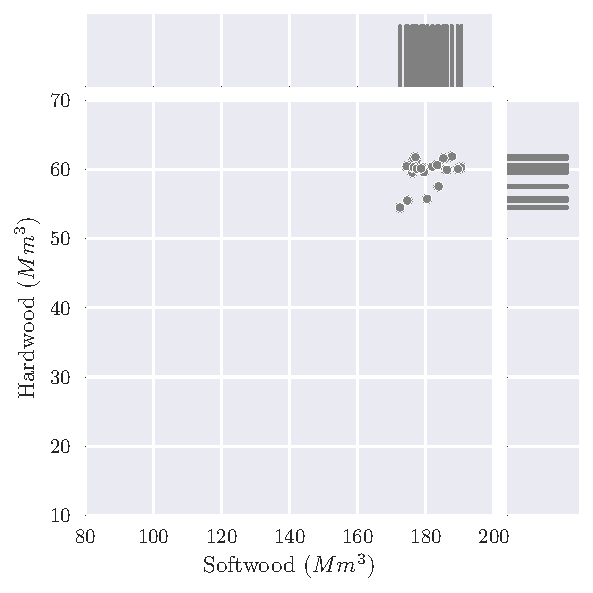
\includegraphics[height=\textwidth]{images/aac_jointplot}
%         \caption{AAC}
%     \end{subfigure}%
%     \begin{subfigure}[t]{0.5\textwidth}
%         \centering
%         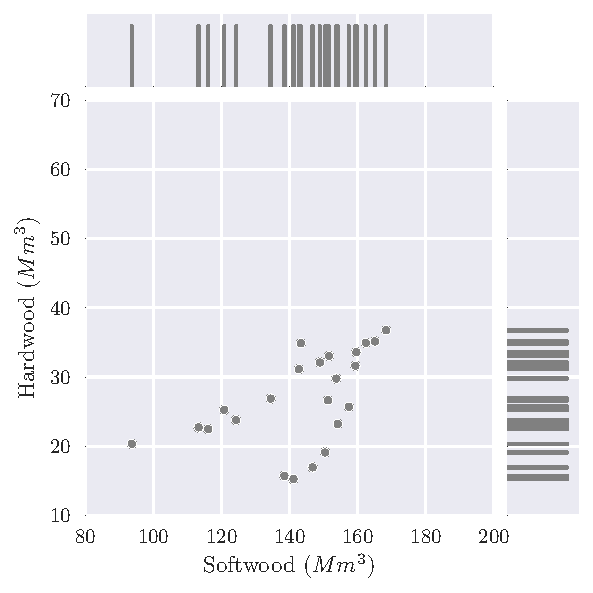
\includegraphics[height=\textwidth]{images/harvest_jointplot}
%         \caption{Harvest Volume}
%     \end{subfigure}
%   \caption{Species-wise joint distributions of AAC and harvest volume for period 1990 to 2012}
%   \label{fig:jointdist}
% \end{figure}


The data show a species-skewed negative consumption bias, relative to AAC, which is related to the infinite-demand assumption implicitly embedded in the classic wood supply optimization model formulation. 
%which is the \emph{de facto} standard tool used by government authorities to determine AAC on Crown land. 
\citet{paradis2013risk} estimate the impact of this bias, using a sequence of 30 two-phase rolling-horizon planning cycles\footnote{The first phase simulates determination of AAC by government officials, and the second phase simulates consumption of a profit-maximizing subset of available fibre by forest products industry firms.}, and show that consuming a species-skewed subset of AAC can induce future wood supply failures under certain conditions. They conclude that the wood supply planning process currently in place on Crown land in Canada does not provide credible assurance of long-term sustainability of the wood supply. Given the pervasiveness of the species-skewed negative consumption bias, the classic wood supply optimization model formulation does not constitute a rational basis for the implementation sustainable forest management. 

%---



% \subsection{Wood Supply Planning}

% \subsection{Principal-agent Problem}

% \subsection{Bilevel Optimization}

For management and planning purposes, the forest landscape is subdivided into \emph{stands}. 
The \emph{stand} is the basic silviculture decision unit, and can be described as a contiguous forested area with uniform vegetation and growth characteristics. 
Projection of future forest condition and fibre availability is based on aggregated result of stand-level growth and yield simulation. 
This requires four distinct types of information: (a) hypothetical detailed inventory of current forest condition (i.e., stand ages and types), (b) hypothetical projection of stand condition over time for each type\footnote{Foresters typically refer to these as \emph{yield curves}.}, (c) hypothetical state transitions induced by stand events (i.e., shift in stand age and stand type), and (d) hypothetical intensity, location and timing of planned future stand events (e.g., clear-cut harvesting of stand $x$ in planning period $i$). 

%High cost of collecting and compiling inventory, yield curve, and transition inputs is matched with heightened awareness of sampling error. 
%Particular attention is paid to minimizing estimation bias \todo{Add references showing research on impact of wood supply model input error.}. 
%Thus, estimation error tends to cancel out for the first three data types \citep{ouhimmou2010robust}. 

Wood supply optimization models typically use the first three information types (i.e., starting inventory, yield curves, and state transitions) as input, leaving the fourth information type (location and timing of future stand events) as variables in the objective function. 
%The c is often obtained from the output of wood supply optimization models. implicitly embedded in the objective function and constraints of the classic wood supply planning model. 
%The implicit nature of the future harvest hypotheses on wood supply analysis has received relatively little attention in the literature. 
Assembling this information into a coherent model, and subsequent analysis of model output, is referred to as the \emph{wood supply planning problem}. 
We focus on a particular problem variant, which we call the \emph{distributed wood supply planning problem}, where the roles of forest land owner and industrial fibre consumer are played by independent agents. 
This is a common situation in Canada and other jurisdictions, where public forest land is managed by government stewards on behalf of the general population.

%\citet{paradis2013risk} present an illustrative case study showing that the common "maximal even-flow harvest volume" wood supply model formulation implicitly assumes that aggregate fibre industrial demand exceeds potential fibre supply throughout the planning horizon. This assumption does not hold in many instances. Using a two-phase iterative simulation, the authors show that systematic over-estimation of harvesting activity in this wood supply model formulation can have a negative impact on both credibility of long-term demonstration of sustainability and stability of industrial fiber supply.

%Based on these findings, we propose to extend the "maximal even-flow harvest volume" wood supply model formulation to include explicit anticipation of industrial fibre consumption behaviour. 

The classic wood supply planning model formulation 
%(see \citet{paradis2013risk} for a detailed description of formulation) 
does not explicitly consider industrial fibre-consumption behaviour. Instead, it implicitly assumes infinite demand (i.e., all harvested fiber will be consumed, regardless of quantity, quality, species, price, or other considerations). This assumption is not coherent with available data in some jurisdictions, where historical fibre consumption is systematically lower than maximum potential wood supply \citep{ccfm2005wood}.  This bias compromises credibility of the wood supply planning process.

We aim to improve the long-term wood supply planning model formulation by explicitly anticipating industrial fibre consumption behaviour. To do so, we can describe the distributed wood supply planning problem, from game-theoretic perspective, as an instance of the principal-agent problem. 
% Stackelberg game \citep{stackelberg2010market, olsder2009phenomena}. 
The role of \emph{principal} is played by the forest owner (or government steward), and the role of \emph{agent} is played by the industrial fibre consumer. 
%Although we embed our model in an iterative simulation framework, we disregard the repeated nature of principal-agent interaction (i.e, we assume a static or ``one shot'' game, with no dynamic evolution of player behaviour induced by game repetition).
%The principal wishes to offer the biggest perpetually-renewable wood supply contract possible. 
%When the principal uses the classic wood supply optimization model, he fails to account for the agent's willingness to consume all the fibre offered.

%%%%%%%%%%%%%%%%%%%%%%%%%%%%%%%%%%%%%%%%%%%%%%%%%%%%%%%%%%%%%
% TO DO: summarize PA in forestry literature...
%%%%%%%%%%%%%%%%%%%%%%%%%%%%%%%%%%%%%%%%%%%%%%%%%%%%%%%%%%%%%

\section{Source of Antagonism}

The principal has the long-term responsibility to ensure a sustained wood supply (hence the even-flow constraints in the wood supply model), but aims to maximize economic activity from exploitation of the forest resource (hence the wood-supply-maximization objective function).
The agent aims to maximize short-term profit from transformation of wood supply into forest products.
Antagonism between the principal and agent is linked to either (a) binding agent capacity constraints or (b) the presence of negatively-valued subsets of the wood supply. 
Either of these factors will prevent the profit-maximizing agent from consuming the entire wood supply, which in turn induces the problematic negative consumption bias described in \citet{paradis2013risk}.

The test dataset used in the computational experiments presented later in this paper features binding agent capacity constraints.
Our test dataset has two lines (which we will refer to as \emph{hardwood} and \emph{softwood}, based on an aggregation of tree species that grow in our test forest).
All the hardwood harvested from the forest must pass through a single hardwood sawmill.
The hardwood sawmill capacity is approximately one third of the maximum sustainable hardwood supply level determined by the principal using the classic wood supply optimization model.
The softwood line is profitable and has sufficient capacity to process the entire softwood supply offered by the principal.
The agent therefore has an incentive to utilize his entire softwood allocation, but limit his hardwood consumption to the capacity of the hardwood sawmill.
We have only permitted clear-cut harvesting in our test model, which means the agent only has take-all and leave-all options for each harvestable forest unit.
In order to achieve the correct hardwood/softwood mix in his harvesting plan, the agent may select harvest units that have a lower proportion of hardwood than the harvest units appearing in the first period of the principal's optimal wood supply solution.
This species-biased deviation from the principal's wood supply plan increases risk of future wood supply shortages.

In the case of wood supply offers with negatively-valued subsets, the only way the principal has to motivate the agent to act is by allowing him to harvest part of the forest (i.e., the agent can choose to consume any subset of wood supply offered by the principal). 
In practice, it is difficult (impossible) for the principal to force the agent to consume timber at a net loss, so this is a real problem. 
The principal is incited to propose plans where part of the output is not interesting for the agent, as this allows him to increase his wood supply offer (this is desirable, given his objective function). 
Including this negatively-valued part in the short-term wood supply allows the principal to increase the long-term wood supply offer\footnote{For example, simulating harvesting of relatively unproductive or over-mature parts of the forest and regenerating them into higher-productivity stands in a wood supply model may increase the availability of fibre in a future time period. This \emph{allowable cut effect} is a well documented forest policy instrument. For more information, see \citet{luckert1995allowable}.}.
However, the agent only plans his consumption on a short-term basis, and has no incentive to consume the negatively-valued subset of wood supply.
It may be impossible for the principal to offer the globally optimal plan \emph{and} force the agent to use all of the wood offered. 
By not consuming the uninteresting part of the supply, the agent may compromise the principal's long term plan.

We illustrate this second source of antagonism with an example. % (see Figure \ref{ref:stablestate}).
Suppose the principal $P$ can offer $H_1$ to the agent $A$, which has a value $v(H_1) = 10M\$$. 
To this offer, the principal can add $H_2$, which has a value $v(H_2) = 2M\$$.
However, $H_1$ and $H_2$ can only be consumed sustainably if they are bundled with $H_3$, which has a value $v(H_3) = -1M\$$. 
The best long-term solution for both parties is for the agent to consume $H_1$, $H_2$ and $H_3$ for $v(H_1 \cup H_2 \cup H_3) = 11M\$$.
However, the principal knows that if he offers all three lots, the profit-maximizing agent will only take $H_1$ and $H_2$ for $v(H_1 \cup H_2) = 12M$.
The principal knows that this is unsustainable, so he only offers $H_1$ which is sustainable but has a lower value of $10M\$$.

Note that if the principal could bundle the uninteresting part with a more interesting surplus, then the antagonism would disappear.
However, this bundling would require a more highly-constrained contract binding the agent to the principal.
This bundling option is not typically available to the principal in practice, leaving him with no rational choice but to lower the wood supply offer until the agent willingly consumes it all.
Determining the maximum species-wise even-flow wood supply offer that will be totally consumed by the agent is not a trivial problem.
The antagonism between the two levels can induce non-convexity in the solution space, when we constrain the principal's problem such that a wood supply contract is principal-feasible only if the agent consumes it entirely.

% \begin{figure}[h]
%   \centering
%   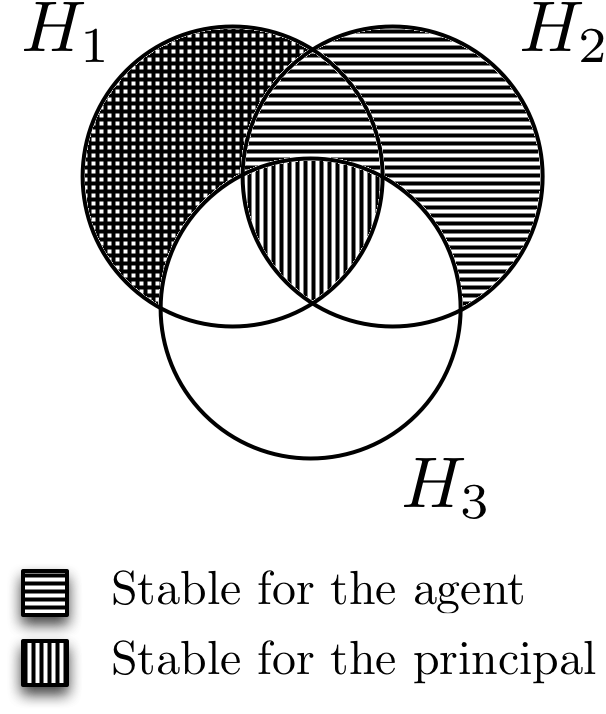
\includegraphics[width=50mm]{images/venn_stablestate}
%   \caption{Illustration of stable state for principal and agent}
%   \label{fig:stablestate}
% \end{figure}

\section{Non-Convexity of Bilevel Solution Space} 

\todo{Should we consider moving the detailed proof to an appendix?}

Before we present a formal mathematical formulation of the bilevel optimization problem, we provide a simple counter-example illustrating potential convexity problems (see Figure \ref{fig:counterexample}). The context for our counter-example is a simple setup where the principal offers a supply of hardwood and softwood to the agent. 
The agent must willingly consume the entire wood supply offer for a given solution to be principal-feasible.

The agent is actually composed of two independent sub-agents (softwood and hardwood lines). 
This is similar to the test dataset used in the computational experiments we present later in this paper.
Each sub-agent maximizes his own profit (i.e., is not willing to reduce his profit for the benefit of the other).
There are three types of transformation processes: boards, paper, and cogeneration.
The \emph{boards} process is equally profitable for both lines ($+50\,\si{\$\per\cubic\metre}$ for both softwood and hardwood), and has a transformation capacity of two input units for each line.
The \emph{paper} process is profitable for both lines, but at different rates ($+50\,\si{\$\per\cubic\metre}$ for the softwood line, $+10\,\si{\$\per\cubic\metre}$ for the hardwood line); it has a transformation capacity of three input units for each line.
The \emph{cogen} process is marginally profitable for for the softwood line ($+1\,\si{\$\per\cubic\metre}$), and marginally unprofitable for the hardwood line ($-1\,\si{\$\per\cubic\metre}$); it has a transformation capacity of one input unit for each line.

Transforming inputs using the paper process requires utilization of a common resource for both lines.
There is a difference in line-wise efficiency for utilization of the common resource.
The softwood line utilizes two units of the common resource for each unit of input transformed, whereas the hardwood line is twice as efficient.
Problems with non-convexity of the solution space may arise when this common resource becomes saturated.

The counter-example starts with a solution offer of $4$ units of softwood and $4$ units of hardwood.
The agent consumes the entire offer, for a profit of $\$320$. 
Consider a slight perturbation that alters the solution by $+2$ units softwood and $-2$ units of hardwood; this produces the globally optimal solution, for a profit of $\$351$. 
We will show that this $(+2S,-2H)$ bundled move, while still increasing the value for the agent, goes outside of the stable solution space.
Next, consider a smaller perturbation that alters the solution by $+1$ unit of softwood and $-1$ unit of hardwood.
In this case, the agent will not consume the entire offer (he will not consume the unprofitable unit of hardwood that would go to the cogen process).
This is an infeasible solution from the perspective of the principal, as the bilevel model formulation requires the principal to consider only wood supply offers that will be entirely consumed by the agent. Given that all three points (i.e., $(0S, 0H)$, $(+1S, -1H)$, $(+2S, -2H)$) located along a line in solution space, infeasibility of intermediate point $(+1S, -1H)$ proves non-convexity\footnote{By definition, given a line segment whose endpoints lie inside a convex space, it is not possible for any point along this line segment to lie outside the convex space. }\todo{Hopefully the footnote clarifies sufficiency of our counter-example as proof of non-convexity of the general problem case.}.

Even the simplest bilevel optimization problems are known to be $\mathcal{NP}$-hard, and non-convex solution spaces are common \citep{dempe2003annotated, colson2007overview}. 

%\todo{Has this condition been clearly defined yet earlier in the text?}

% The the prototype for this methodology was developed under the incorrect assumption that the solution space for combined problem P3 was convex.
% In fact, the solution space for problem P3 is non-convex, which is common in bilevel programs \citep{dempe2003annotated}.

\begin{figure}[H]
  \centering
  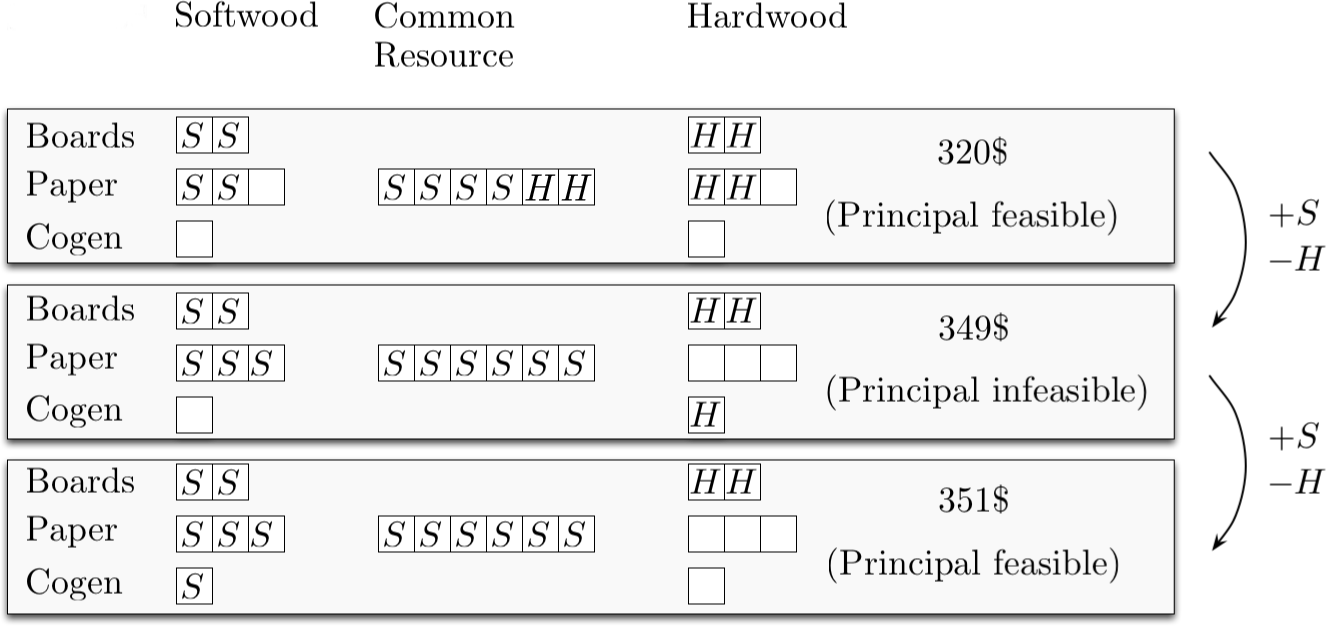
\includegraphics[width=\textwidth]{images/counterexample_edited2}
  \caption{Simple counter-example illustrating non-convexity of bilevel problem solution space}
  \label{fig:counterexample}
\end{figure}


% From olsder2009phenomena:
% In [13], one can for instance read: “It is a remarkable feature of these problems (i.e., contract design games) that the leader always takes all, pushing the follower to zero utility”.
% 13. Selanie, B.: The Economics of Contracts. MIT Press, Cambridge (2000)
%
% This seems to be the case for our model as well; the principal pushes the agent to the break-even point in an effort to maximize AAC.

%We show that tightening the gap between planned and implemented harvesting activities improves both credibility and performance of the distributed wood supply planning process.

\section{Mathematical Formulation}
\label{sec:formulation2}

This section describes the bilevel optimization problem formulation. We use the bilevel programming terminology found in \citet{colson2007overview}.

\subsection{General Case}

We present a mathematical formulation for the general case. First, we define some symbols which will be used to formulate the principal and agent models.

\begin{align*}
\intertext{Let}
\Theta &\colonequals  \text{set of extreme principal feasible solutions}\\
\Phi &\colonequals  \text{set of extreme agent feasible solutions}\\
O &\colonequals \text{the set of forest outputs}\\
R &\colonequals \text{set of resources}\\
\gamma_{\theta,o} &\colonequals \text{quantity of output $o \in O$ produced by the principal solution $\theta \in \Theta$}\\
\alpha_{\phi,r} &\colonequals \text{quantity of resource $r \in R$ consumed by the agent solution $\phi \in \Phi$}\\
\delta_{\phi,o} &\colonequals \text{quantity of output $o \in O$ consumed by the agent solution $\phi \in \Phi$}\\
v_{\theta} &\colonequals \text{value of solution $\theta \in \Theta$ for the principal}\\
w_{\phi} &\colonequals \text{value of solution $\phi \in \Phi$ for the principal}\\
g_{\phi} &\colonequals \text{value of solution $\phi \in \Phi$ for the agent}\\
u_r &\colonequals \text{maximal amount of resource $r \in R$}\\
\intertext{represent the parameters, and}
 x_{\theta} &\colonequals \text{proportion of the final principal solution built from principal solution $\theta \in \Theta$}\\
y_{\phi} &\colonequals \text{proportion of the final agent solution built from agent solution $\phi \in \Phi$}\\
\mu_o &\colonequals \text{dual price of output $o \in O$}\\
\pi_r &\colonequals \text{dual price of resource $r \in R$}\\
\intertext{represent the variables.}
\end{align*}

\begin{align} 
  \intertext{The primal formulation of the agent's optimization problem is}
    z_A(x) \colonequals \boldsymbol{\max} \sum_{\phi \in \Phi} g_{\phi} y_{\phi} \\
    \shortintertext{\textbf{subject to} \nonumber} \\
     \sum_{\phi \in \Phi} \alpha_{\phi,r} y_{\phi} & \leq u_r , & \forall r \in R \\
     \sum_{\phi \in \Phi} \delta_{\phi,o} y_{\phi} & \leq d_o = \sum_{\theta \in \Theta} \gamma_{\theta,o} x_{\theta} , & \forall o \in O \\
     \sum_{\theta \in \Theta} x_\theta & = 1 \\
     \sum_{\phi \in \Phi} y_\phi & = 1 \\
     y & \geq 0 \\
    \intertext{The dual formulation of the agent's optimization problem is}
   z_A(x) \colonequals \boldsymbol{\min} \sum_{r \in R} u_r \pi_r + \sum_{o \in O} d_o \mu_o \\
    \shortintertext{\textbf{subject to} \nonumber} \\
     \sum_{r \in R} \alpha_{\phi,r} \pi_r + \sum_{o \in O} \delta_{\phi,o} \mu_o & \geq  g_{\phi} , & \forall \phi \in \Phi \\
    \pi, \mu & \geq 0 
\end{align}

The global solution is stable for both the principal and the agent if the following condition is met, expressing equality of output production (by the principal) and output consumption (by the agent).

\begin{equation}
\sum_{\phi \in \Phi} \delta_{\phi,o} y_{\phi}  = \sum_{\theta \in \Theta} \gamma_{\theta,o} x_{\theta}
\end{equation}

A stable formulation can be obtained by combining the primal and dual agent problems, and requiring equality on the output consumption constraint.

\begin{align} 
    z_A(x) \colonequals \boldsymbol{\max}  \sum_{\phi \in \Phi} g_{\phi} y_{\phi} \\
    \shortintertext{\textbf{subject to} \nonumber} \\
    \sum_{\phi \in \Phi} \alpha_{\phi,r} y_{\phi}  - s_r  & = u_r, & \forall r \in R \\
    \sum_{\phi \in \Phi} \delta_{\phi,o} y_{\phi} & = \sum_{\theta \in \Theta} \gamma_{\theta,o} x_{\theta} , & \forall o \in O \\
    \sum_{r \in R} \alpha_{\phi,r} \pi_r + \sum_{o \in O} \delta_{\phi,o} \mu_o - \sigma_\phi  & = g_{\phi} , & \forall \phi \in \Phi \\
     s_r \pi_r & = 0 , & \forall r \in R \\
    \sigma_{\phi} y_{\phi} & = 0 , & \forall \phi \in \Phi \\
    \sum_{\theta \in \Theta} x_\theta & = 1 \\
    \sum_{\phi \in \Phi} y_\phi & = 1 \\
    y, \pi, \mu & \geq 0 
\end{align}

We can formulate the principal's optimization problem by modifying the objective function to express the sum of principal and agent solution values, from the perspective of the principal.

\begin{align} 
    z_A(x) \colonequals \boldsymbol{\max}  \sum_{\theta \in \Theta} v_{\theta} x_{\theta} + \sum_{\phi \in \Phi} w_{\phi} y_{\phi} \\
    \shortintertext{\textbf{subject to} \nonumber} \\
    \sum_{\phi \in \Phi} \alpha_{\phi,r} y_{\phi}  - s_r  & = u_r, & \forall r \in R \\
    \sum_{\phi \in \Phi} \delta_{\phi,o} y_{\phi} & = \sum_{\theta \in \Theta} \gamma_{\theta,o} x_{\theta} , & \forall o \in O \\
    \sum_{r \in R} \alpha_{\phi,r} \pi_r + \sum_{o \in O} \delta_{\phi,o} \mu_o - \sigma_\phi  & = g_{\phi} , & \forall \phi \in \Phi \\
     s_r \pi_r & = 0 , & \forall r \in R \\
    \sigma_{\phi} y_{\phi} & = 0 , & \forall \phi \in \Phi \\
    \sum_{\theta \in \Theta} x_\theta = 1 \\
    \sum_{\phi \in \Phi} y_\phi = 1 \\
    y, \pi, \mu & \geq 0 
\end{align}

\subsection{Special Case}

As discussed earlier, the general case for this bilevel problem is non-convex. 
However, there is a special case of this problem, which we can solve to global optimality. 
Non-convexity problems arise in the agent's problem when at least one convergent node in the network has a saturated capacity constraint. 
The special case is simply the inverse of the problematic case, and occurs in two types of instances: (a) strictly divergent networks, and (b) general networks with sufficient capacity at convergent nodes that these will not be saturated. 
The first sub-case (i.e., strictly divergent flows) can be identified by analyzing network topology. 
The second sub-case may only be observable through empirical analysis. 
Figure \ref{fig:cases} illustrates these cases graphically. 

\begin{figure}[h]
  \centering
  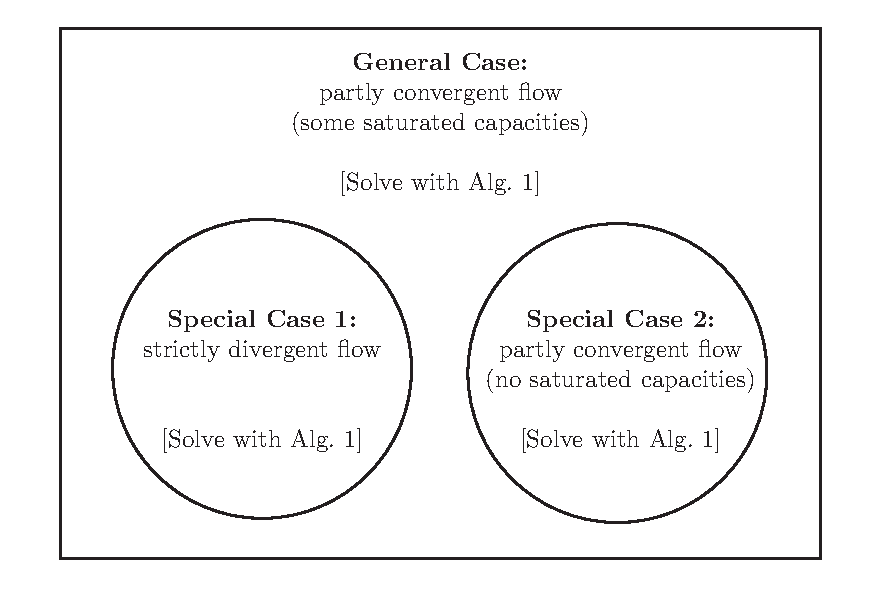
\includegraphics[width=\textwidth]{images/cases}
  \caption{Graphical illustration of problem cases}
  \label{fig:cases}
\end{figure}

We present a mathematical formulation for the special case. First, we present four additional parameter definitions

\begin{align*}
\Phi_o &\colonequals  \text{set of extreme agent feasible solutions for output $o \in O$}\\
%\gamma_{\theta,o} &\colonequals \text{quantity of output $o \in O$ produce by the principal solution $\theta \in \Theta$}\\
\alpha_{\phi_o,r} &\colonequals \text{quantity of resource $r \in R$ consumed by the agent solution $\phi_o \in \Phi_o$}\\
\delta_{\phi_o,o} &\colonequals \text{quantity of output $o \in O$ consumed by the agent solution $\phi_o \in \Phi_o$}\\
g_{\phi_o} &\colonequals \text{value of solution $\phi_o \in \Phi_o$ for the agent}\\
\intertext{and four additional variable definitions}
y_{\phi_o} &\colonequals \text{proportion of the final agent solution built from agent solution $\phi_o \in \Phi_o$}\\
\sigma_{\phi_o} &\colonequals \text{dual price of limit $o \in O$ for agent solution $\phi_o \in \Phi_o$} \\
\mu_{\phi_o} &\colonequals \text{dual price of output $o \in O$ for agent solution $\phi_o \in \Phi_o$}\\
\pi_r &\colonequals \text{dual price of resource $r \in R$}\\
\end{align*}

We can now formulate the special case of the agent's optimization problem as follows, decomposing the general case problem into output-wise subproblems.

\begin{align} 
  \intertext{The primal formulation of the agent's optimization problem is}
    z_A(x) \colonequals \boldsymbol{\max} \sum_{o \in O} \sum_{\phi_o \in \Phi_o} g_{\phi_o} y_{\phi_o} \\
    \shortintertext{\textbf{subject to} \nonumber} \\
    \sum_{o \in O} \sum_{\phi_o \in \Phi_o} \alpha_{\phi_o,r} y_{\phi_o} & \leq u_r , & \forall r \in R \\
    \sum_{\phi_o \in \Phi_o} \delta_{\phi_o,o} y_{\phi_o} & \leq 1 , & \forall o \in O \\
    \sum_{\phi_o \in \Phi_o} y_{\phi_o} & \leq d_o = \sum_{\theta \in \Theta} \gamma_{\theta,o} x_{\theta} , & \forall o \in O \\
    \sum_{\theta \in \Theta} x_\theta & = 1 \\
    \sum_{\phi_o \in \Phi_o} y_\phi & = 1, & \forall o \in O\\
    y & \geq 0\\
    \intertext{The dual formulation of the agent's optimization problem is}
   z_A(x) \colonequals \boldsymbol{\min} \sum_{r \in R} u_r \pi_r + \sum_{o \in O} d_o \mu_o \\
    \shortintertext{\textbf{subject to} \nonumber} \\
    \sum_{r \in R} \alpha_{\phi,r} \pi_r + \sum_{o \in O} \delta_{\phi,o} \mu_o & \geq  g_{\phi} , & \forall \phi \in \Phi \\
    \pi, \mu & \geq 0 
\end{align}

Similarly to the general case, we can derive a bilevel problem formulation that is stable for both the principal and the agent, by requiring equality on the output consumption constraint.

\begin{align} 
    z_A(x) \colonequals \boldsymbol{\max}  \sum_{o \in O} \sum_{\phi_o \in \Phi_o} g_{\phi_o} y_{\phi_o} \\
    \shortintertext{\textbf{subject to} \nonumber} \\
    \sum_{o \in O} \sum_{\phi_o \in \Phi_o} \alpha_{\phi_o,r} y_{\phi_o}  - s_r  & = u_r, & \forall r \in R \\
    \sum_{\phi_o \in \Phi_o} \delta_{\phi_o,o} y_{\phi_o} & = \sum_{\theta \in \Theta} \gamma_{\theta,o} x_{\theta} , & \forall o \in O \\
    \sum_{o \in O} \sum_{r \in R} \alpha_{\phi_o,r} \pi_r + \sum_{o \in O} \delta_{\phi_o,o} \mu_o - \sigma_{\phi_o}  & = g_{\phi_o} , & \forall o \in O, \phi_o \in \Phi_o \\
    s_r \pi_r & = 0 , & \forall r \in R \\
    \sigma_{\phi_o} y_{\phi_o} & = 0 , & \forall \phi_o \in \Phi_o \\
    \sum_{\theta \in \Theta} x_\theta & = 1 \\
    \sum_{\phi_o \in \Phi_o} y_{\phi_o} & = 1 & \forall o \in O \\
    y, \pi, \mu & \geq 0 
\end{align}

We can formulate the principal's optimization problem by modifying the objective function to express the sum of principal and agent solution values, from the perspective of the principal.

\begin{equation} 
    z_A(x) \colonequals \boldsymbol{\max} \sum_{o \in O} \sum_{\theta \in \Theta} v_{\theta} x_{\theta} + \sum_{\phi_o \in \Phi_o} w_{\phi_o} y_{\phi_o} \\
\end{equation} 
\begin{align} 
    \shortintertext{\textbf{subject to} \nonumber} \\
    \sum_{o \in O} \sum_{\phi_o \in \Phi_o} \alpha_{\phi_o,r} y_{\phi_o}  - s_r  & = u_r, & \forall r \in R \\
    \sum_{\phi_o \in \Phi_o} \delta_{\phi_o,o} y_{\phi_o} & = \sum_{\theta \in \Theta} \gamma_{\theta,o} x_{\theta} , & \forall o \in O \\
    \sum_{o \in O} \sum_{r \in R} \alpha_{\phi_o,r} \pi_r + \sum_{o \in O} \delta_{\phi_o,o} \mu_o - \sigma_{\phi_o}  & = g_{\phi_o} , & \forall o \in O, \phi_o \in \Phi_o \\
    s_r \pi_r & = 0 , & \forall r \in R \\
    \sigma_{\phi_o} y_{\phi_o} & = 0 , & \forall \phi_o \in \Phi_o \\
    \sum_{\theta \in \Theta} x_\theta & = 1 \\
    \sum_{\phi_o \in \Phi_o} y_{\phi_o} & = 1 & \forall o \in O \\
    y, \pi, \mu & \geq 0 
\end{align}


\section{Solution Methodology}

We originally set out to design an iterative solution methodology for the general case, based on the pioneering work of \citet{fortuny1981representation} and \citet{bard1982explicit}, however convexity issues limited this approach to local optimal solutions. 
Consequently, we decided to focus our algorithmic development efforts on special cases which we could solve to global optimality.

By limiting the problem domain to the special cases, we eliminate the possibility of interaction between outputs $o \in O$.
The optimal solution to the lower-level problem can then be described as the sum of optimal solutions to output-wise sub-problems.  
This property allows us to compute output-wise upper bounds on agent consumption behaviour.
These upper bounds can subsequently be used to optimally constrain the upper-level problem.
This is the basis of our solution methodology for the special case.
Algorithm \ref{alg:bilevel_specialcase} describes the solution methodology using pseudo-code.

\vspace{12pt}
\begin{algorithm}[H]
  \DontPrintSemicolon
  \SetKwInOut{Output}{Output}
  \Output{Global optimal wood supply solution $x^*$}
  \BlankLine
  \ForEach{output $o \in O$} {
    Determine upper bound $u_o = z_P^o$ on agent consumption of output $o$ (i.e., solve integrated sub-problem with all non-targeted outputs disabled). \;
  }
  \ForEach{output $o \in O$} {
    Set upper bound constraint $\gamma_o \leq u_o$ on quantity of output $o$ produced by the upper level of the integrated master problem. \;
  }
  Solve integrated master problem. \;
  \caption{Bilevel model solution algorithm (special case: no saturated joint capacity constraints)}
  \label{alg:bilevel_specialcase}
\end{algorithm}
\vspace{12pt}

Algorithm \ref{alg:bilevel_generalcase} describes an algorithm to solve the general case to global optimality by simple enumeration (i.e., iterate over the set of all possible convex subproblems, and return the best solution). Algorithm 2 is of limited practical interest, as computational effort required to solve realistically-sized instances by enumeration would be prohibitive. Efficiency of the general algorithm could potentially be improved by replacing subproblem enumeration with a custom branching algorithm taking advantage of problem structure, however we have not tested this approach.

\vspace{12pt}
\begin{algorithm}[H]
  \DontPrintSemicolon
  \SetKwInOut{Output}{Output}
  \Output{Global optimal wood supply solution $x^*$}
  \BlankLine
  \ForEach{output $o \in O$}{
    Generate subproblem (isolate output $o$ in lower-level problem). \;
    Solve subproblem. \;
    }
  Sum subproblem solutions. \;
  Build super-saturated process set $P_s$ (i.e., find violated capacity constraints). \;
  \ForEach{combination of super-saturated process $p \in P_s$ and output $o \in O$} {
    Generate subproblem (restrict certain combinations of output $o$ and process $p$). \;
    Solve subproblem. \;
    \If{subproblem feasible (i.e., no violated capacity constraint)} {
        Add solution $x$ to feasible solution set $X$. \;
    }
  }
  \Return{Global optimal solution $x^*$ (i.e., best solution in feasible set $X$).} \;
  \caption{Bilevel model solution algorithm (general case: saturated joint capacity constraints)}
  \label{alg:bilevel_generalcase}
\end{algorithm}
\vspace{12pt}

The bilevel model can be solved to global optimality with relative ease when lower level input datasets have some special properties. 
The test dataset used in our test simulations corresponds to special case 2.
Special case 1 occurs if the product lines (i.e., outputs $o \in O$) in the lower level model are totally independent (i.e., strictly divergent). 
Before elaborating further on this condition, we will describe the lower level data model in a bit more detail.

The lower level data model can be described as a network of abstract processors connected by product flows.
Figure \ref{fig:abstract_process} presents a graphical representation of an abstract processor node.
An abstract process consumes inputs and resources, and produces outputs.

\begin{figure}[h]
  \centering
  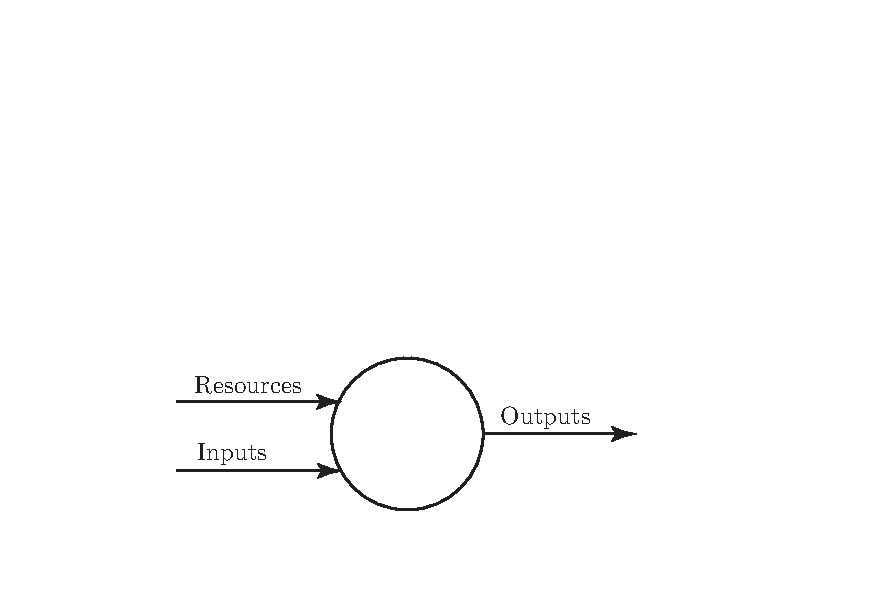
\includegraphics[width=70mm]{images/abstract_process}
  \caption{Graphical representation of an abstract process}
  \label{fig:abstract_process}
\end{figure}
 
At the upstream (source) end of this network is the interface between upper and lower level models. 
Output from the first planning period in the upper level model (i.e., outputs $o \in O$) becomes input material that can be transformed by the lower-level network. 
At the downstream (sink) end of the lower level network, external clients are willing to pay set unit prices to satisfy a bounded demand for each end product. 
This end client demand enables the model to generate profits by pulling a subset of available fibre supply through the network to satisfy a (profit-maximizing) subset of end client demand.
When raw upper-level model outputs are first pulled into the lower network, they must go through one of several front-line processor nodes that convert the raw wood supply into species-wise assortments of logs. 
These front-line processors simulate the interface between the forest and the mills (i.e., the process of harvesting and delivering logs to mills, including transportation cost, which can vary depending on the forest zone from which the raw volume inventory was picked).

Raw upper-level volume is classified by species, and this species-wise distinction may (optionally) be maintained as the outputs are pulled into the lower-level network, depending on configuration of front-line processors. 
For example, in the case of our test dataset, the front-line processors are configured to convert raw upper-level volume into assortments of either hardwood or softwood logs of various sizes \footnote{Our upper-level dataset uses a more fine-grained classification of tree species, which is aggregated into \emph{hardwood} and \emph{softwood} log types by the front-line processors.}.

Due to the abstract nature of the lower-level processor implementation, it is possible to simulate any combination of divergent and convergent product flows. 
Strictly divergent networks correspond to special case 1, and can be solved to global optimality using Algorithm \ref{alg:bilevel_specialcase}. 
Special case 2 occurs when the network includes convergent product flows, but no joint capacity constraints are saturated. 
Although somewhat more difficult to detect, special case 2 is not problematic and can also be solved to global optimality using Algorithm \ref{alg:bilevel_specialcase}.
For special cases 1 and 2, each product line $o \in O$ can be treated as an independent subproblem. 
The optimal value of $z_{A_o} (x)$ for output $o$ is equal to $\argmax_{v_o} p(v_o)$, where $p(v_o)$ is a concave function describing profit for any non-negative consumption volume $v_o$ (see Figure \ref{fig:pvo}). 
%This corresponds to the maximum volume that the agent can be expected to consume for a given product line $o$, which we use as an upper bound on harvest level for product line $o$ in the final step of Algorithm \ref{alg:bilevel_specialcase}. 

\begin{figure}[h]
  \centering
  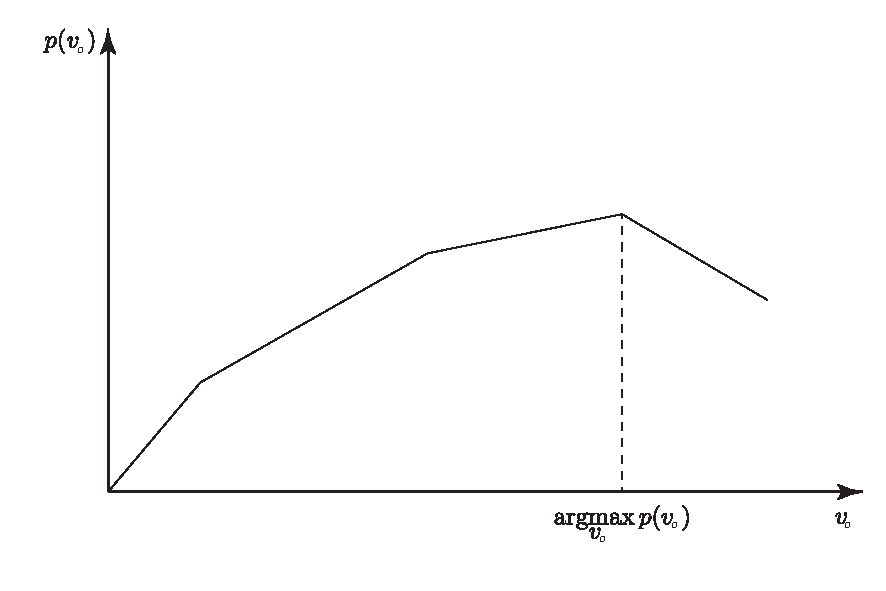
\includegraphics[width=\textwidth]{images/pvo}
  \caption{Illustration of concave profit function of a hypothetical product $o$}
  \label{fig:pvo}
\end{figure}

%For special cases 1 and 2, the profit functions are implicitly embedded in the dataset. 
The product-wise subproblems can be represented using the lower-level model by disabling all non-targeted outputs\footnote{Non-targeted outputs can be disabled by manipulating input parameters of the upper level model, setting conversion efficiency and conversion cost of front-line processors to null values. Instead of converting wood supply units to log assortments, the modified front-line processors now consume all non-targeted outputs at zero cost, which blocks non-targeted outputs from further flow through the lower-level model network.}. 
We can then easily solve each subproblem to obtain the optimal sub-problem solutions without having to explicitly locate intermediate inflection points of profit function $p(v_o)$. 
This corresponds to the maximum volume that the agent can be expected to consume for a given output $o$, which we use as an upper bound on harvest level for output $o$ in the final step of Algorithm \ref{alg:bilevel_specialcase}.

Note that output from our bilevel model is structurally identical to output from the classic model (i.e., output-wise upper bounds on harvest levels, bundled with required levels of pre-commercial sylviculture treatments). 
Thus, our bilvel model can potentially be used as a drop-in replacement for the single level model.
\todo{Is this really not clear?}
%We test this using a case study, which we describe in the next section.

%\section{Computational Experiment}
\section{Materials and Methods}

This section describes the computational experiments we conducted to compare performance of classic and bilevel wood supply models.

\subsection{Description of Dataset}

We tested our bilevel solution methodology on a realistic synthetic dataset from Quebec, Canada.
The study area is a forest management unit (FMU 031-53) located in the boreal forest region of the province of Quebec, Canada. It covers an area of approximately 102 040 hectares. 
%The forest inventory data for this area was compiled into a number of management strata for the purposes of wood supply modeling.  
Approximately (88\%) of initial growing stock is from softwood species, with the remaining (12\%) of initial growing stock in hardwood species. 
Although some pure softwood stands are present, forest cover is dominated by mixed-wood stands containing different proportions of
hardwood mixed in with the softwood. See \citet{paradis2013risk} for a more detailed description of the study area.

Output from the upper-level (forest) model is aggregated into two outputs: \emph{softwood} and \emph{hardwood}. 
The lower-level (industrial) model has limited capacity for transforming hardwood (approximately $1/3$ of potential sustainable wood supply). 
%The upper level model has a single (clearcut) harvest treatment implemented, which has the effect of ``bundling'' hardwood and softwood together in the upper-level model solution.
%A combination of limited hardwood processing capacity in the lower level and output bundling in the upper level indirectly constrains softwood consumption in the lower level.
The classic wood supply model therefore systematically over-estimates short-term hardwood fibre consumption.

% We have not thus far succeeded in developing a solution methodology that guarantees convergence on global optimality for the general convergent case with saturated capacity constraints 
% However, we have developed an iterative solution methodology that we believe could converge on locally optimal solutions in a finite number of iterations. 
% Our methodology for the general case relies on iterative shadow price feedback from the lower level to guide selection of new columns to add to the basis in a column-generation--based algorithm embedded in the upper level. 
% We have not yet implemented or tested the solution methodology for the general case.

%See \citep{paradis2013risk} for a detailed description of case study dataset.  
We use the same test dataset as in \citet{paradis2013risk}, which is an instance of special case 2. Although chip flows from both hardwood and softwood sawmills converge at the pulp mill, we have determined empirically that its capacity is sufficient to avoid saturation problems.

\subsection{Simulation Framework}

We use the two-phase rolling-horizon simulation framework developed by \citet{paradis2013risk} as a testbed in which to compare the long-term performance classic and bilevel wood supply model formulations. 
%This framework uses agency theory to model interaction between government wood supply planners (the \emph{principal} and industrial fibre consumers (the \emph{agent}.

% assumes that long-term AAC-maximizing wood supply planning is controlled by government planners (the \emph{principal}), and that short-term profit-maximizing fibre consumption is controlled by industry planners (the agent). 
The principal and the agent make their moves sequentially, in a two-phase game, repeated 30 times. The framework simulates forest growth between each 5-year rolling-horizon re-planning cycle. The principal has the advantage of the first move, which means he can set AAC to any level of his choosing. Thus, the simulation results presented here show the cumulative result of 150 years of iterative replanning, under different combinations of principal and agent behaviour. 

% We tested our bilevel model within the simulation framework presented in \citet{paradis2013risk}. This framework models the wood procurement planning cycle as a two-phase process, which allows us to simulate principal-agent interaction and simulate rolling the long-term planning horizon forward one period.


\subsection{Experimental Methodology}
\label{sec:experimental_methodology2}

We present six scenarios, showing impact of replacing the classic wood supply model with the bi-level wood supply model. Within any given scenario, simulation parameters for the industrial fibre consumption network\footnote{Mill capacities, costs, prices, client demand, etc.} are held constant for all 30 planning cycles. 
%Table X summarizes the key simulation parameters for each scenario. 

Scenario 1 simulates \emph{status quo} behaviour for both principal and agent, and acts as a control scenario. At each planning cycle, the principal maximizes even-flow AAC (30-period horizon) using the classic wood supply model, then the agent maximizes first-period profits (1-period horizon) by consuming the optimal subset of the wood supply offered by the principal. The principal does not consider the agent's fibre consumption capacity when determining AAC. 

Scenario 2 presents a perfect-implementation bilevel scenario; rather than being allowed to re-plan harvesting on a one-period horizon, the agent is forced to exactly implement the first period of the principal's bilevel wood supply solution. This scenario shows the best-case performance of the bilevel model solution, and is equivalent to the principal controlling the entire wood procurement process from stump to mill gate.

Scenario 3 is the basic bilevel scenario. The principal uses the bilevel model to determine AAC, and the agent is allowed to replan harvesting on a one-period horizon, choosing the profit-maximizing subset of available wood supply. Due to the optimal formulation of the bilevel model and perfect anticipation of volume consumption, the agent always chooses to harvest the entire wood supply. However, the agent may select to harvest this volume from a different combination of forest types than what was prescribed in the first period of the principal's optimal solution. This reflects the distributed nature of forest management planning on Crown land in many jurisdictions.

The contrast between scenario 1 and scenario 2 shows the sensitivity of long-term wood supply to deviations from the principal's optimal wood supply plan.

Scenarios 4 and 5 simulate reducing the softwood supply allocated to the agent to 80\% and 60\% of AAC. Adjusting AAC allocation indirectly creates a buffer stock to protect against decreases in wood supply induced by agent harvest re-planning (i.e., compensation for the principal's incomplete control of the fibre procurement process).

Scenario 6 shows the effect of simulating centralized agent fibre procurement planning on long-term wood supply. For this scenario, we relax the agent's line-wise profitability contraint, and allow him to maximize total network profit. For this scenario, we allow any overflow fibre (hardwood, in our case) to be disposed of at a moderate unit cost. This allows the agent's softwood line to subsidize the disposal of excess hardwood from harvesting of mixed-wood stands, thereby increasing the agent's total potential fibre consumption. This in turn relaxes the lower-level consumption constraints in the principal's bilevel model, thereby allowing him to increase the wood supply offer without compromising long-term sustainability. 

%Scenarios 2 through 6 replace the classic wood supply model with with bilevel model. These scenarios show the long-term cumulative impact of anticipating industrial fibre consumption behaviour within the AAC-determination process. 

%Scenarios 1, 3, 4 and 5 simulate standard agent behaviour; the agent is allowed to select any available forest units for harvesting in the first period, subject to species-wise AAC upper-bound constraints. The agent harvests the entire wood supply for both species groups. This is expected behaviour, given that we simulate perfect anticipation of agent behaviour (i.e., we use the same optimization model formulation for both the agent-anticipation constraint embedded into the bilevel model, and for simulation of agent consumption behaviour in the second phase of the rolling-horizon replanning simulation, as in \citet{paradis2014bilevel}. Note that although the the anticipation mechanism embedded into the bilevel model perfectly anticipate the \emph{volume} of fibre consumption, these may be harvested from different forest units than than the ones that make up the basis of the first period of principal's optimal wood supply solution. This reflects the distributed nature of forest management planning on Crown land.

%Scenario 2 forces the agent to exactly implement the principal's first-period optimal solution. This is an optimistic scenario, to illustrate the best-case performance of the bilevel model solution.


% We present a computational experiment using two scenarios (control and test). 
% The purpose of the computational experiment is to show convergence of our solution methodology, and to compare solution times (i.e., computational effort) between control and test scenarios.

% The \emph{control} scenario corresponds to the \emph{status quo} (i.e., our best attempt at simulating current principal and agent behaviour).
% The \emph{test} scenario uses the bilevel model (instead of the classic model) to simulate the principal's behaviour in the first stage of each planning cycle; all other parameters are held constant. 
% %The purpose of the computational experiment is to show that our solution methodology for the special case of the bilevel problem converges quickly on a globally optimal solution, using a dataset of realistic size and complexity.

% For each planning cycle, principal and agent each get to make their move sequentially. 
% First the principal maximizes even-flow wood supply (30-period horizon), then the agent maximizes first-period profits (1-period horizon).
% %Planning horizon length is 30 periods for the first (principal) phase, and 1 period for the second (agent) phase.  
% Planning period length is 5 years.
% The test scenarios presented in this paper show results from a single two-phase planning cycle.

% Note that we simulate \emph{perfect} anticipation of agent behaviour, by using identical model formulations for both the agent-anticipation mechanism (in the first phase of the simulation) and the agent-execution mechanism (in the second phase of the simulation).
% This helps clearly illustrate convergence of the solution methodology under best-case conditions.

% %We present results from a single cycle of the two-phase wood supply planning problem (i.e., principal determines sustainable wood supply, agent consumes profit-maximizing subset of the wood supply).  

% %Long-term effect of the bilevel formulation, after repeated planning cycles, will be presented in a future publication. 


\section{Results}
\label{sec:results2}

We present experimental results in two stages. First, we show detailed results comparing output from the first planning cycle of scenarios 1 and 2. Next, we show result of simulating 30 rolling-horizon planning cycles for scenarios 1 to 6.

Figure \ref{fig:scenarios_detail} presents detailed results from the first planning cycle of scenarios 1 (control) and 3 (bilevel).
 
For the control scenario, potential hardwood fibre supply is 64\,583\,\si{\cubic\metre}, whereas actual consumption is only 20\,800\,\si{\cubic\metre}.
The difference between planned and executed hardwood fibre consumption volumes is due to the limited processing capacity at the (single) hardwood sawmill in the lower-level model.
The entire softwood fibre supply is consumed by the agent, as we would expect, as both end-product demand and processing capacity for the softwood line are high enough to accommodate more softwood fibre than the forest can supply. 
This phenomenon (of consuming certain components of the wood supply entirely while other components are only partially consumed) can be observed to varying extents in practice, where processing capacity and market demand are often misaligned with the proposed wood supply.

In order to harvest the full softwood supply volume while only harvesting a third of the hardwood supply, the agent must favour forest stands that have a high proportion of softwood (low proportion of hardwood).
The wood supply model is sensitive to deviation from the timing and location of harvesting activities prescribed in the first period of the optimal solution.
Even slight deviations from the optimal solution carry a high risk of rendering the solution infeasible (from the perspective of the principal, in the form of wood supply shortages) in future periods.   
This is inherently problematic, as the optimal solutions from wood supply models were never intended to be implemented as-is\footnote{Intended usage of wood supply model solutions is limited to estimating species-wise upper bounds on short-term timber licence allocations, such that long-term sustainability of the wood supply is not irreversibly compromised.
Producing an operationally feasible fibre procurement plan (including access road construction and maintenance, harvesting, transportation, and follow-up silviculture treatments) from the first period of the wood supply plan requires considerable dis-aggregation and refinement.}.

%\footnote{Wood supply modelling is considered a long-term planning exercise. Consequently, wood supply models are highly simplified representations of the complex interactions between forest growth and anthropogenic disturbances (i.e., harvesting). Input data is highly aggregated.}

Thus, minimizing the gap between planned and executed harvesting volume should help reduce the risk of future wood supply failures.
The primary motivation for developing the bilevel model formulation presented here is to proactively mitigate selective wood supply consumption behaviour. 
We implement this idea by embedding explicit anticipation of industrial fibre consumption into the wood supply model, such that the principal offers the maximal sustainable wood supply that will be entirely consumed by the agent. 
Re-defining the wood supply problem in this way improves the quality of linkage between strategic and tactical planning levels.

%Although the upper-level wood supply model uses a 30-period horizon to predict future wood supply, these model are typically used on a 1-period rolling-horizon (i.e., the model is re-run at the beginning of each planning period). 

Results show that our bilevel anticipation mechanism completely eliminates over-estimation of hardwood fibre consumption volume. 
Fibre consumption by the agent is exactly equal to wood supply volumes offered by the principal (20\,800\,\si{\cubic\metre} for hardwood, and 323\,759\,\si{\cubic\metre} for softwood ).
This is the desired outcome from the bilevel model, and represents a global optimal solution for this instance. Note that the agent plans his own harvesting in the second stage of the planning cycle (using his single-period profit-maximizing model), so harvest areas will not typically match the first period of the principal's plan, even if harvest volume is exactly equal.  
%, given that our test dataset is an instance of special case 2 (i.e., convergent network with non-saturated shared resource). 

\begin{figure}[H]
  \centering
  \medskip
  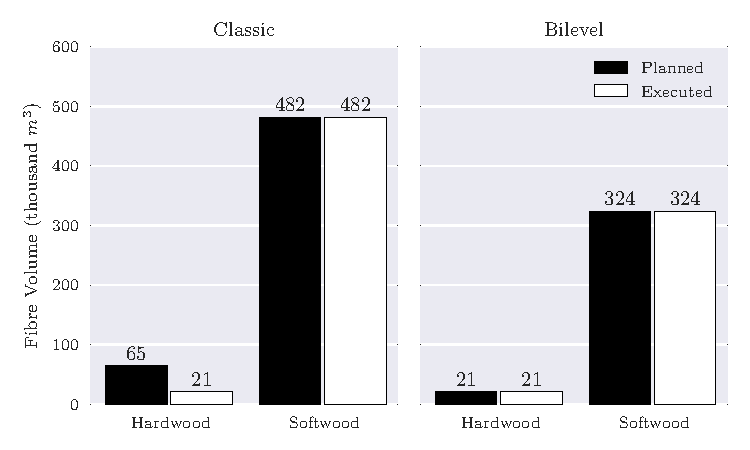
\includegraphics[width=\textwidth]{images/article2_compbar}
  \caption{Comparison of planned and executed volumes}
  \label{fig:scenarios_detail}
\end{figure}

Table \ref{tab:scenarios} presents intermediate results from each step of the bilevel solution method (see Algorithm \ref{alg:bilevel_specialcase}).
We present this data to show how we derive the optimal upper bounds to the wood supply problem from solutions to output-wise sub-problems.
Hardwood consumption capacity (20\,800\,\si{\cubic\metre}) is the binding constraint in this case. 
Our anticipation mechanism shows that the softwood line could have profitably consumed up to 584\,861\,\si{\cubic\metre} of softwood in the first planning period, however the species-wise even-flow constraints on the upper-level wood supply model limit long-term softwood harvest level to 323\,759\,\si{\cubic\metre}.
As expected, the agent's fibre consumption volume in the second phase of the simulation is exactly equal to the wood supply.
This shows that the bilevel model eliminates the gap between planned and executed fibre consumption levels, thereby fulfilling its intended purpose.

\begin{table}
\caption{Bilevel solution method Intermediate results}
\label{tab:scenarios}
\renewcommand{\tabcolsep}{2pt}
\begin{tabular}{llrr}
\toprule 
Phase & Description & \multicolumn{2}{c}{Volume (\si{\cubic\metre})} \tabularnewline
&& Hardwood & Softwood \tabularnewline
\midrule
1 (principal) & Upper bound on \emph{hardwood} consumption & 20\,800 & - \tabularnewline
1 (principal) & Upper bound on \emph{softwood} consumption & - & 584\,861 \tabularnewline
1 (principal) & Maximum even-flow wood supply levels & 20\,800 & 323\,759 \tabularnewline
2 (agent) & Agent fibre consumption & 20\,800 & 323\,759 \tabularnewline
\bottomrule
\end{tabular}
\end{table}

The classic model can be solved in a single step.
This corresponds to approximately 13 seconds of CPU time to solve classic wood supply model for the first (of 30) planning cycle in scenario 1.
For scenario 2, the bilevel model requires $\left|O\right| + 1$ steps to solve.
This corresponds to approximately $(4 + 6) + 10$ seconds of CPU time using our test setup.
We ran our tests on an Intel\textsuperscript{\textregistered} Xeon\textsuperscript{\textregistered} E5-2670 processor (20\,\si{\mega\byte} cache, 2.60 \si{\giga\hertz}).

Figures \ref{fig:scenarios} shows simulation results the six scenarios described in the previous section. For each scenario, Figure \ref{fig:scenarios}(a) plots species-wise AAC and fibre consumption for each of the 30 rolling-horizon re-planning cycles simulated. The same data are shown in Figure \ref{fig:scenarios}(b) using box-plots to illustrate the variability of period AAC and fibre consumption values across scenarios. The boxes encompass the inter-quartile range (IQR) with the median marked. The whiskers extend to $1.5 \text{IQR}$ past the closest quartile; any observations outside this range are marked as outliers using a dot symbol.


\begin{sidewaysfigure}%
  \centering
  \subfloat[][]{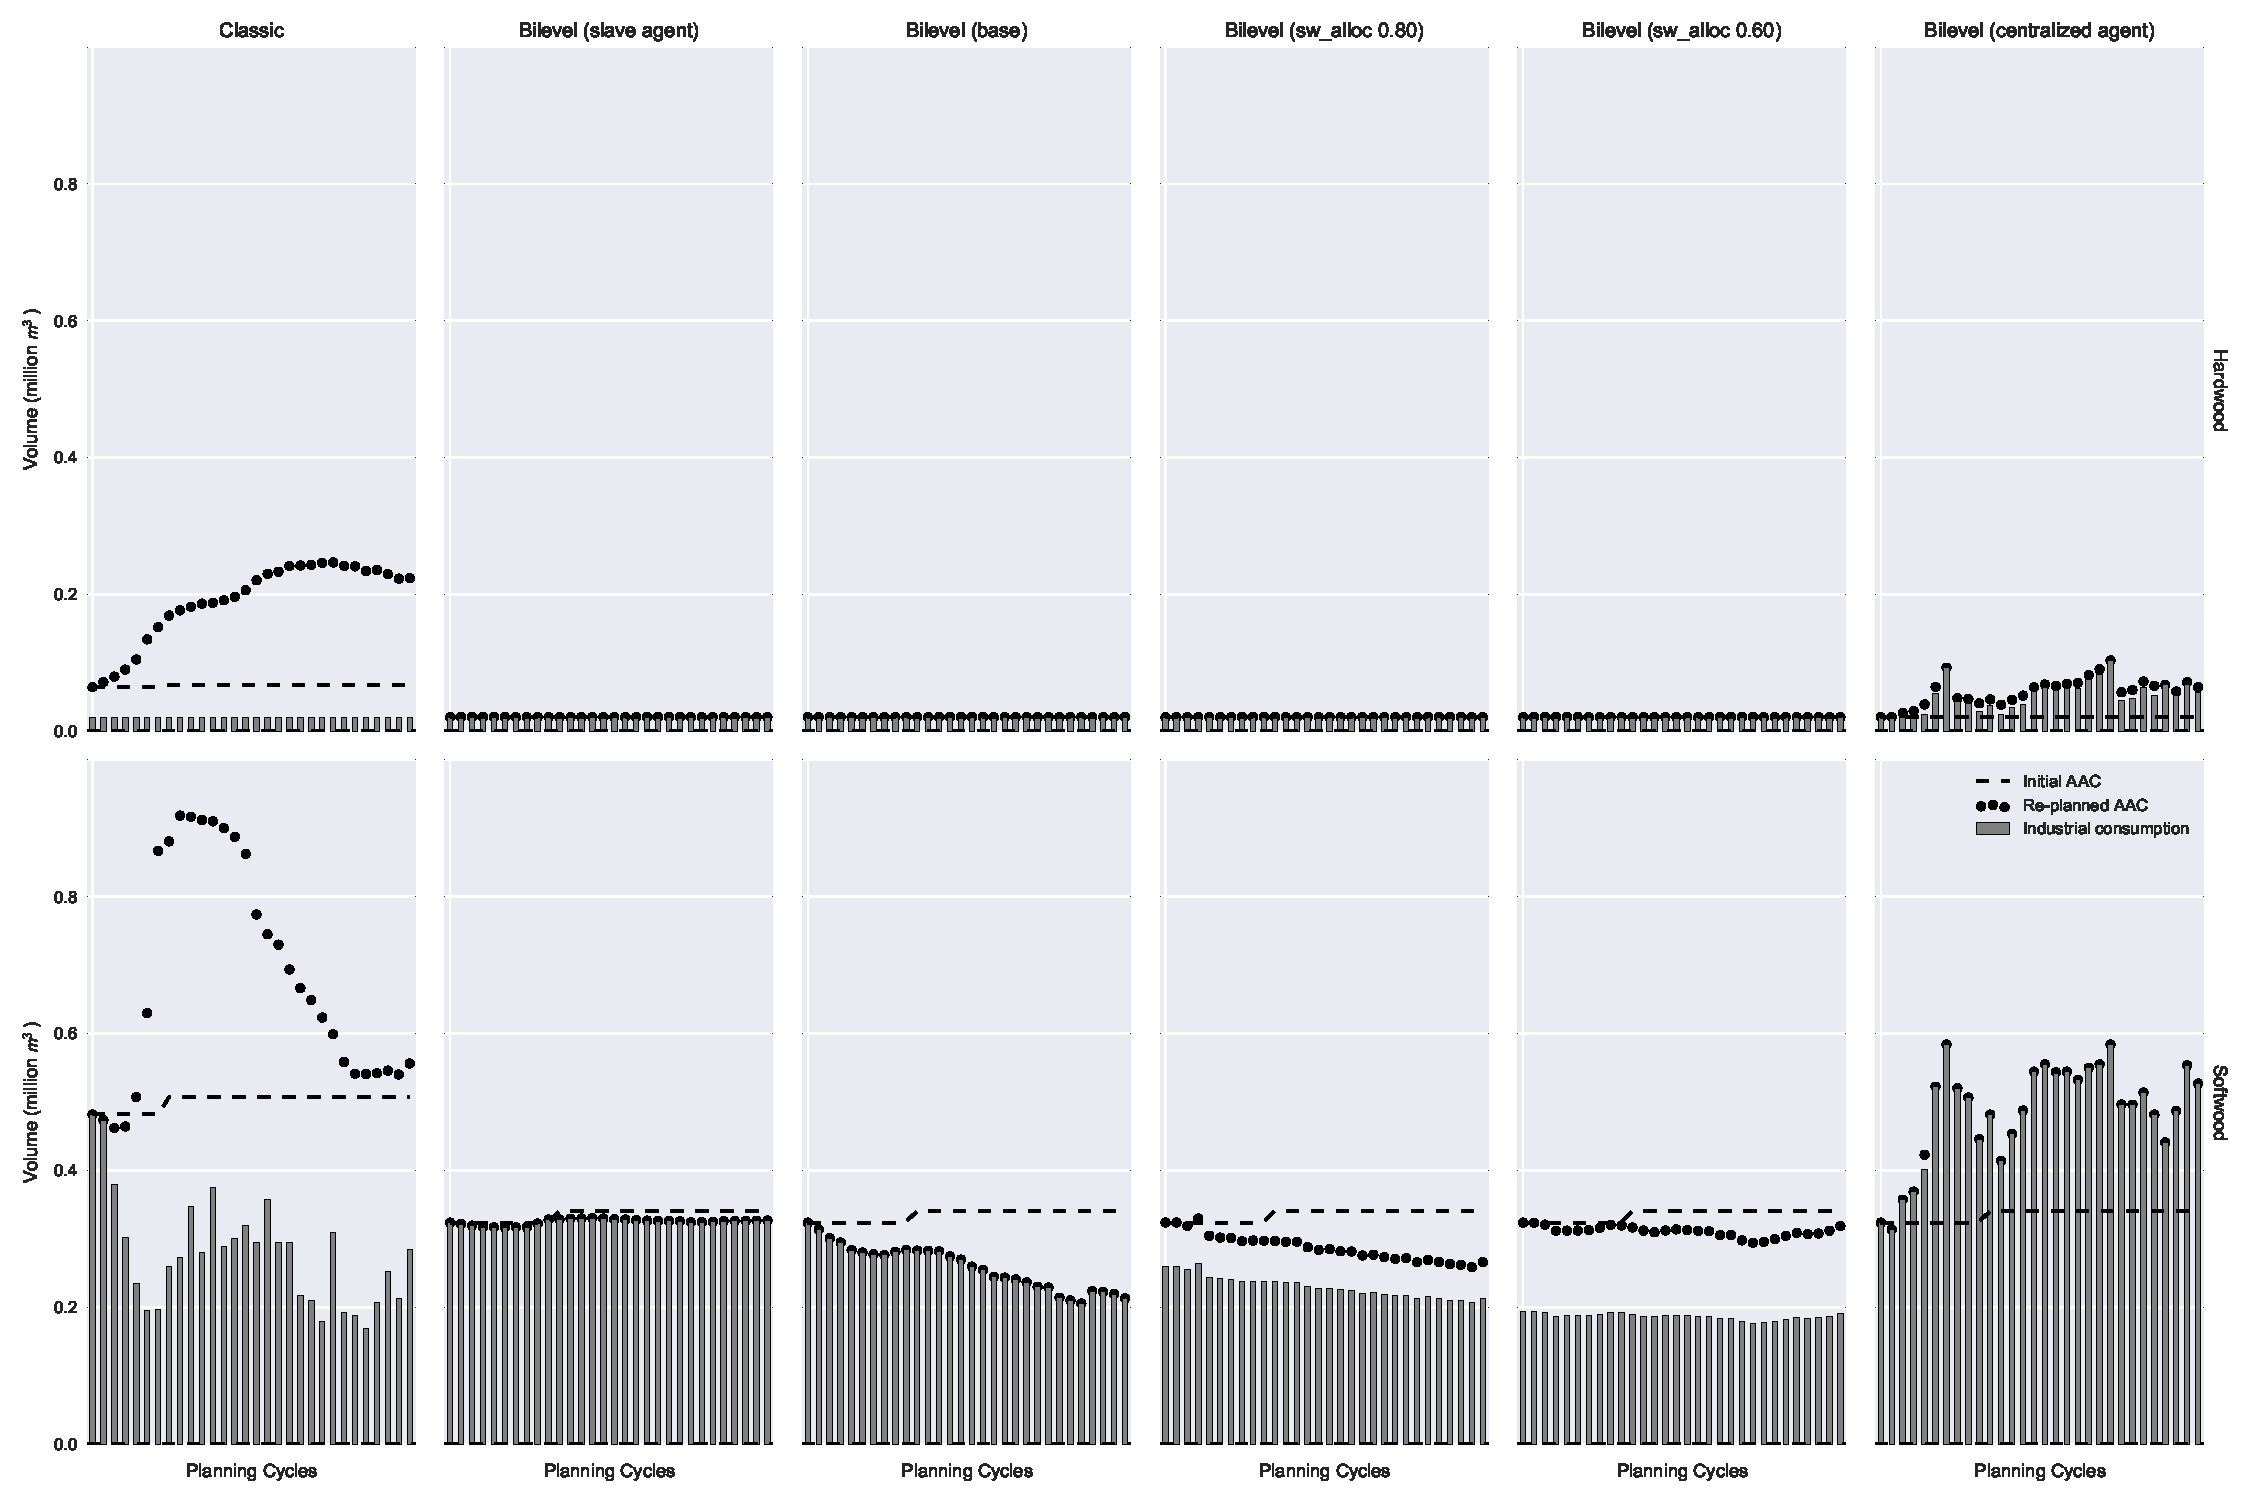
\includegraphics[width=\textwidth]{images/scenarios_timeseries}}%
  \caption{Species-wise AAC and fibre consumption for scenarios 1 to 6 (time series)}%
  \label{fig:scenarios}%
\end{sidewaysfigure}

\begin{sidewaysfigure}%
  \ContinuedFloat
  \centering
  \subfloat[][]{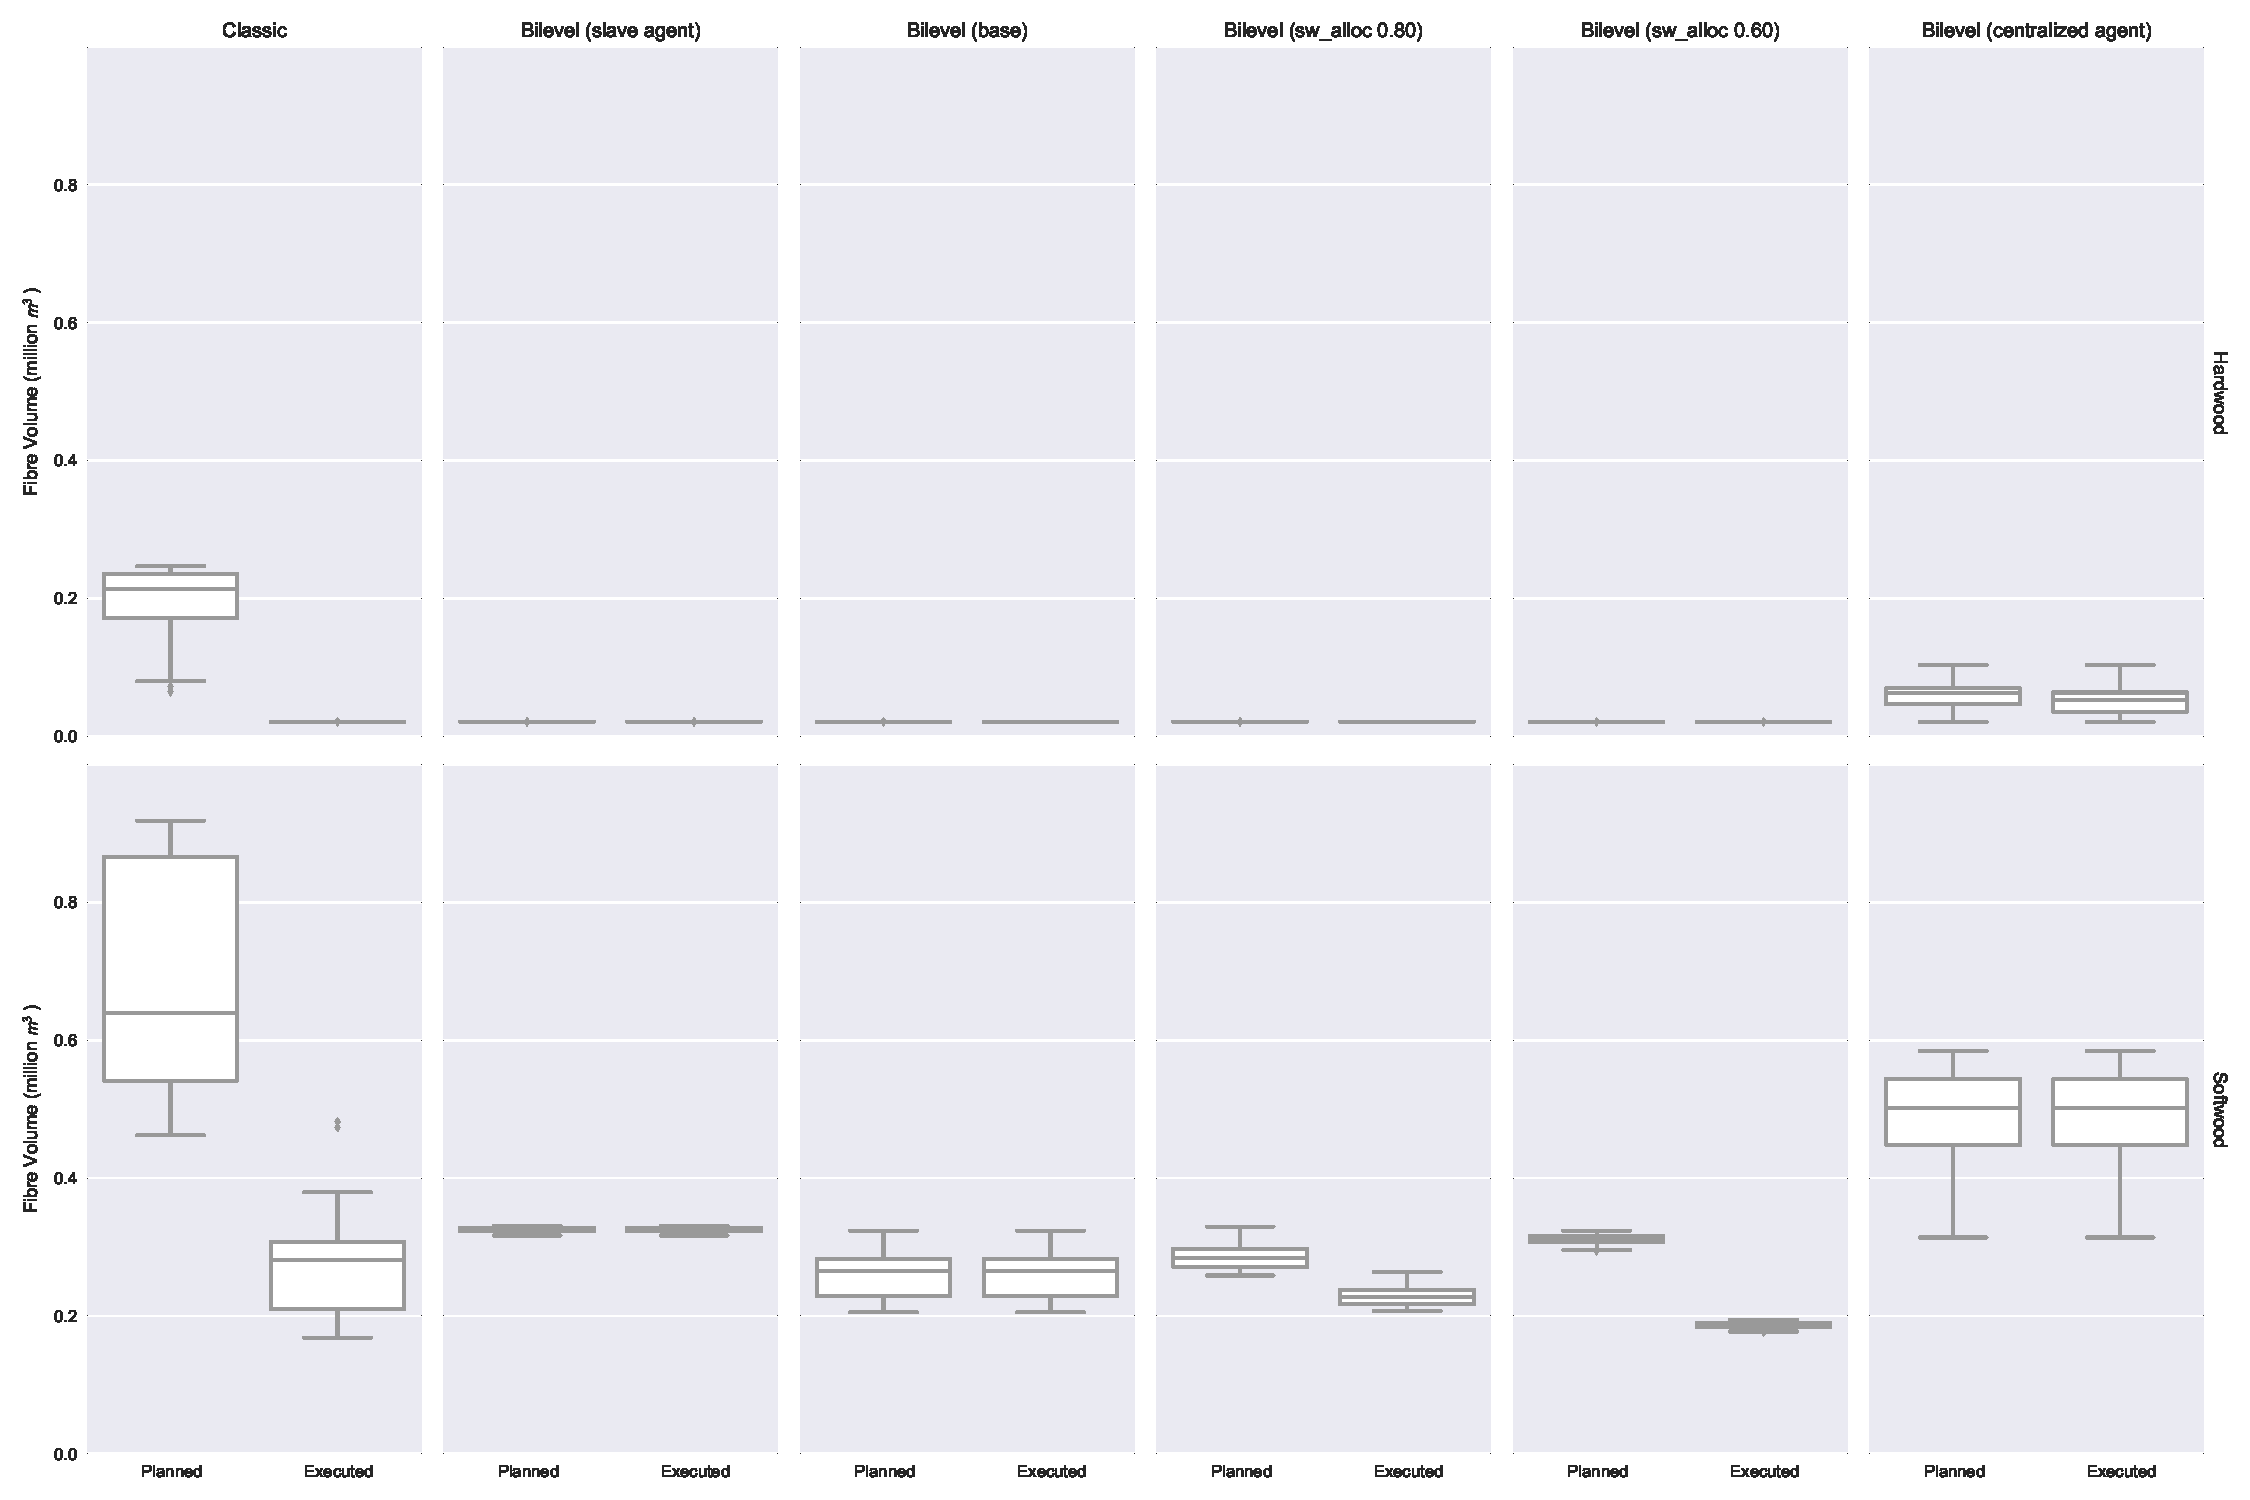
\includegraphics[width=\textwidth]{images/scenarios_boxplots}}%
  \caption{Species-wise AAC and fibre consumption for scenarios 1 to 6 (boxplots)}%
  %\label{fig:scenarios_plot}%
\end{sidewaysfigure}

%\begin{figure}%
%  \ContinuedFloat
%  \centering
%  \subfloat[][]{...figure code...}%
%  \caption[]{Species-wise AAC and fibre consumption for scenarios 1 to 6 (boxplots)}%
%  \label{fig:scenarios}%
%\end{figure}


\section{Discussion}
Scenario 1 shows the relative instability of the classic wood supply model. This is attributable to the species-skewed gap between AAC and fibre consumption volumes. Despite the harvest levels being systematically lower than AAC, the agent's preference for harvesting high-softwood-content stands gradually shifts the composition of the residual forest cover towards a higher hardwood content. \citet{paradis2013risk} use the term \emph{systematic drift effect} to describe this phenomenon.   

The principal uses the bilevel model to determine AAC for scenarios 2 through 6. By virtue of its formulation, the bilevel model completely eliminates the volume gap between AAC and fibre consumption. Note that we simulate perfect anticipation of agent fibre consumption \emph{volume}. For scenarios 3 through 6, we allow the agent to plan his own harvesting in the second phase of each planning cycle simulation; this explains the residual instability in long-term wood supply for scenarios 3 and 4.

Scenario 2 forces the agent to harvest the exact forest units that form the basis of the first period of the principal's optimal bilevel solution. The purpose of this scenario is to show that wood supply tracks almost perfectly along the initial bilevel AAC solution (even after 30 rolling-horizon re-planning cycles) under best-case conditions (i.e., when the principal controls wood procurement planning execution all the way to the mill gate). In practice, the decoupling point between the principal and the agent is not typically located this far downstream; scenarios 3 through 6 simulate a more conventional decoupling point.

Scenario 3 shows vastly improved stability (hence credibility) of the softwood supply levels, relative to the control scenario. Note the slight, but monotonic, downward trend of the softwood fibre supply for scenario 3. As discussed earlier, the contrast between scenarios 2 and 3 shows that the bilevel model is sensitive to even slight deviations the optimal wood supply model solution. This type of sensitivity to deviations from the optimal solution is typical of deterministic optimization models, as optimal solutions are invariably located along the boundary of the feasible region; even the slightest deviations from the optimal solution (or error in the constraint right-hand-side values) can induce problem infeasibility.

Scenarios 4 and 5 show the effect of reducing the proportion of AAC that is allocated to the agent, in an attempt to compensate for the residual drift seen in scenario 3. Reducing allocation is an indirect way for the principal to induce a buffer stock in the standing timber inventory. This tends to move the agent's solution away from the feasible boundary of the principal's solution space, thereby improving the robustness of the distributed wood supply planning process. Scenario 4 shows a marked reduction in drift compared with scenario 3. Residual drift is virtually eliminated in scenario 5, but at the expense of 40\% of the maximum potential (bilevel) sustainable wood supply. 

Intuitively, foregoing 40\% of the potential wood supply seems like a high price to pay to eliminate the residual drift in a bilevel modelling context. A more direct management approach to maintaining a buffer stock in standing timber inventory, as described in \citet{raulier2014increasing}, may be a more efficient approach to reducing the residual drift in a distributed wood supply planning context. 

By stabilizing the long-term wood supply, scenario 5 succeeds in restoring credibility to the wood supply planning process, albeit at a relatively high cost in terms of the magnitude of the wood supply. Furthermore, scenario 5 makes less optimistic assumptions regarding agent behaviour than scenarios 2 and 6. Also, it is the only scenario in this series to respect the even-flow pattern prescribed by the wood supply model constraints.  Assuming that the even-flow constraints are valid and necessary (although not sufficient) conditions for sustainability of the forest management plan\footnote{There has been considerable debate in the literature over the validity and necessity of including even-flow or non-declining yield constraints in wood supply optimization models. Nonetheless, one or the other of these constraint formulations has traditionally been included in almost all wood supply models in Canada, since the advent of use of linear programming to optimize wood supply planning (with the notable exception of the proving of Ontario). We have included even-flow constraints in both the classic and bilevel optimization model formulations used in this study, as this allows us to measure the impact of extending the \emph{status quo} wood supply model formulation to include explicit anticipation of industrial fibre consumption behaviour. For more information on the the effects of even-flow constraints and alternative model formulations, we invite the reader to consult \citet{luckert2005should}.}, and that the principal's responsibility to ensure sustainability must absolutely supersede his desire to maximize wood supply allocation, scenario 5 represents the only example of a principal-feasible policy in this study. As mentioned previously, a more efficient buffer stock policy implementation could possibly maintain a similar level of long-term robustness while increasing short-term wood supply allocation level beyond that which we were able to simulate in scenario 5.

% Scenario 6 shows the potential benefit of relaxing the agent's line-wise profitability constraint. This simulates a more centralized fibre procurement behaviour in the agent than the standard agent behaviour simulated in scenarios 2 through 5. Scenario 6 allows the agent to maximize the sum of profits from both hardwood and softwood lines. This opens up the possibility for the agent to dispose of excess hardwood fibre supply (at a moderate cost) in order to gain access to significant extra volume of softwood from previously-inaccessible high-hardwood-content mixed-wood stands. The cost of disposing of the relatively small volume of excess hardwood fibre is offset by the profits from processing and sale of a relatively large volume of newly-available softwood fibre. 

% This increase in hardwood fibre consumption has a positive-feedback effect on long-term fibre supply; the principal may now harvest the problematic mixed-wood stands at a faster in the first few planning cycles. These mixed-wood stands (which where left standing in previous scenarios) can now be replaced with pure softwood plantations. In the medium term, this has the effect of partially re-aligning the inventory of standing timber with industrial fibre demand. In practice, agent behaviour more closely resembles the greedy agent behavior simulated in scenarios 1 through 6.

% Centralized fibre procurement planning almost double average fibre consumption (92\% increase) relative to scenario 3 (i.e., base bilevel scenario). This significant increase in potential fibre consumption represents an important opportunity of the agent, however implementing intra-agent collaborative fibre procurement behaviour is between the is beyond the control of the principal. There is nonetheless a clear incentive for the principal for lobby the agent to align his fibre consumption capacity with the potential wood supply. 

We simulate the distributed wood supply planning process as a two-step sequential game, where the principal proposes his wood supply in the first phase and the agent consumes a profit-maximizing subset of the wood supply in the second phase. Within this context, the bilevel model clearly outperforms the classic model, as shown by the restoration of wood supply stability in scenario 5, albeit at a high cost in terms of short-term fibre allocation.

We conjecture that further increases in sustainable wood supply may even be possible if the principal and the agent were allowed to iteratively adjust their respective supply and demand offers within a given planning cycle. This represents a promising direction for further wood supply policy research. From a game-theoretic perspective, extending the two-stage game simulated in this study to include an iterative negotiation dimension corresponds to a \emph{repeated game} or \emph{supergame} in game theory. Under certain conditions \emph{supergames} are known to converge on \emph{socially optimum} equilibrium solutions (i.e., collaborative solutions) that are globally superior to the (optimal) selfish behaviour in the context of non-repeated (i.e., one-shot) games \citep{fudenberg1991game}. 

The concept of supergames could also be used on a larger scale, to model principal and agent anticipation of upcoming planning cycles (and, potentially, memory of past planning cycles). Ultimately, both scales could be nested (i.e., iterative negotiation within each planning cycle, combined with anticipation of upcoming planning cycles). Although technically challenging, these hypothetical nested-supergame models might be harnessed for practical application using a \emph{metagaming} approach \citep{howard1971paradoxes}, potentially providing a wealth of valuable insight to guide high-level government policy-makers.

Although considerable effort would be required to validate and compile the necessary input data for the agent-anticipation mechanism in a production setting, this data is nonetheless readily available. In the hypothetical local absence of adequate input data for the agent-anticipation mechanism, the principal could adopt a publicly-transparent policy of posing relatively conservative fibre demand assumptions. This would provide the agent with the incentive to collaborate with the principal (by sharing more accurate data). Re-running the wood supply model immediately could provide instantaneous positive feedback to the agent, in the form of increased wood supply.

%We can conjecture that further improvement in the magnitude and stability of the principal's bilevel wood supply solutions could be attained if the industrial fibre consumption capacity of the agent was adjusted such that he could profitably consume the forest's maximum sustainable biophysical fibre production capacity. 

% The centralized behaviour what is typically observed in  approach to 

% , however average wood supply and profit are reduced by approximately 6\% relative to status quo. Figure 3 shows a second bi-level scenario, where we simulate alternate agent behaviour (i.e., centralized management of hardwood and softwood procurement within the industrial agent). Harvest volume and profit are increased well beyond status quo levels, illustrating potential benefit of collaborative fibre procurement planning, although wood supply is more volatile than in the base bi-level scenario.

% All three scenarios simulate a static agent, whose fibre consumption behaviour is poorly aligned with the wood supply. Re-aligning industrial fibre consumption capacity to the forest is key to accessing the full potential wood supply.  A promising area for further research would be concurrent re-designing of both wood supply and industrial capacity to maximize value creation potential. 

Our computational experiment is conducted using a dataset from Quebec, Canada, however our bilevel model concept could be applied to wood supply planning problems in other jurisdictions with similar context (i.e., distributed planning environment with fibre demand). The concept could also be extended to other industries where a distributed, sequential planning process requires anticipation of downstream planning processes. For example, a bilevel modelling approach has recently been used to analyse fisheries quota policies \citep{vandijk2014solving}.
 

\section{Conclusion}
\label{sec:conclusion2}

\citet{paradis2013risk} conclude that the classic wood supply model formulation should be extended to anticipate industrial fibre consumption. 
We frame this problem using agency theory, and propose mathematical formulations to describe the optimization problems of the principal and the agent. 
We then combine principal and agent problems into a bilevel optimization model. 

Using a counter-example, we show that the general case of the bilevel problem is non-convex.
We present a solution algorithm to solve the general case to global optimality, through enumeration of feasible solutions.
However, an enumeration-based strategy is computationally intractable for realistically-sized instances.
By imposing a restrictive condition on the topology of the agent's problem, we isolate a special case of the bilevel problem. The special case can be decomposed into output-wise convex subproblems.
We present a decomposition-based solution algorithm that solves the special case to global optimality.

In practice, many networks correspond to the special case. 
Problematic cases can always be modelled as instances of special case 2, by relaxing binding capacity constraints on convergent nodes such that the shares resources are not saturated.
In many instances, the benefits of explicitly anticipating the agent's behaviour should out-weight any negative side-effects from the aforementioned capacity constraint relaxations.

Lastly, we test our solution methodology on a test dataset of realistic size and complexity, and compare results to output from the classic (single-level) wood supply optimization model. 
Results show that the bilevel solution algorithm for the special case converges on a global optimal solution in less than twice the time required to solve the classic (single-level) model formulation.
Considering that these wood supply models need only be solved once every 5 years, this increase in solution time is deemed insignificant.
The bilevel model can therefore be considered a potential drop-in replacement for the classic model.  

%A more in-depth analysis of principal-agent interaction under bilevel modelling will be presented in an upcoming publication. Further computational experiments will compare long-term effect of using our bilevel model formulation (after repeated rolling-horizon planning cycles) on magnitude and stability of the wood supply.

This study compares the long-term performance of two wood supply optimization model formulations, within the context of the distributed wood supply planning problem. Using a series of six scenarios, we show that the bilevel model improves long-term wood supply stability. 

The bilevel model has the same output data as the classic model and can be solved using comparable computational effort. As such, the bilevel model formulation constitutes a technically adequate and conceptually superior alternative to the classic model.  We recommend that government wood supply planning authorities consider adopting a bilevel modelling approach, as this would improve the credibility of the (currently incredible) sustainable forest management process. 

We examine the performance of a bilevel model formulation in the context of a two-stage principal-agent game. We also recommend that research effort on bilevel wood supply model formulations be extended to \emph{supergame} contexts, both in terms of intra-cycle principal-agent negotiations, and inter-cycle anticipation of future wood supply planning games. To cope with the complexity of using these hypothetical nested-supergame models in a practical government-policy-setting environment, we suggest the adoption of a metagaming approach to wood supply planning as an appropriate starting point for further research. 

\section{Acknowledgements}
\label{sec:acknowledgements2}

This study was supported by funding from the \emph{FORAC Research
  Consortium} and the \emph{Fonds de recherche du Qu\'{e}bec -- Nature
  et technologies}. 


%%% Local Variables: 
%%% mode: latex
%%% TeX-master: "article2_article"
%%% End: 


\bibliographystyle{plainnat}
\bibliography{phd}

%%% Local Variables: 
%%% mode: latex
%%% TeX-master: "909303058"
%%% End: 
\include{article3_chapter}
\setcounter{secnumdepth}{3} 

%\chapter{Restoring credibility to distributed wood supply planning: a case stud}
%\chapter{Improving Coherence of Forest Management Planning Using a Principal-Agent Approach}
\chapter{Sensitivity Analysis}

\pagebreak

\selectlanguage{francais}

\begin{abstract}
  French abstract goes here.
\end{abstract}

%\pagebreak

\selectlanguage{english}

\begin{abstract}
  English abstract goes here.
\end{abstract}

\pagebreak

In Chapter 1, we introduce a two-stage rolling-horizon re-planning simulation framework. Using this framework and a realistic test dataset, we simulate \emph{status quo} interaction between the principal (i.e., government steward of Crown forest) and the agent (i.e., industrial fibre consumer). We conclude Chapter 1 by observing that the classic wood supply optimization model formulation does not predict wood supply failures under certain circumstances\footnote{Specifically, the classic wood supply model fails to predict wood supply failures when industrial fibre consumption is a species-skewed subset of AAC.}, and conjecture that risk of wood supply failures could be mitigated by extending the classic wood supply model to explicitly anticipate industrial fibre consumption behaviour.

In Chapter 2, we present a bilevel wood supply model formulation that anticipates fibre consumption, and develop a solution algorithm to solve a special case of the problem to global optimality. We compare performance of classic and bilevel wood supply models using the simulation framework and test dataset introduced in Chapter 1. We conclude that the bilevel model successfully mitigates risk of wood supply failure, although there is some residual instability in long-term wood supply. 

Note that for our case study test dataset, we simulate a tension between hardwood and softwood fibre consumption. Although the simulation results presented here cannot be directly generalized to other cases, our rolling-horizon simulation framework and bilevel modelling methodology could potentially provide valuable insight into long-term sustainability of wood supply for a range of common problem instances. For example, some areas are characterised by asymmetrical industrial demand between spruce and fir\footnote{Spruce tends to be more highly valued as a raw material for lumber than fir, primarily due to longer kiln-drying times required to produce fir lumber with the targeted final moisture content.}, which would induce principal-agent problems similar to the one described in our case study.

In this chapter, we explore sensitivity of long-term wood supply to various simulation parameters. Using our two-stage rolling-horizon re-planning simulation framework, each scenario simulates 30 planning cycles. Scenarios are grouped into five series, with each series testing different levels of a given parameter. 

All simulation results presented in this chapter use the test dataset described in Chapter 1. Unless specified otherwise, all scenarios use the bilevel model to determine wood supply at each planning cycle and simulate perfect anticipation of agent fibre consumption volume. 

The reference scenario for all series is the base bilevel scenario\footnote{For the reference scenario, the principal uses the bilevel model to determine AAC, and the agent is allowed to replan harvesting on a one-period horizon, choosing the profit-maximizing subset of available wood supply. Due to the optimal formulation of the bilevel model and perfect anticipation of volume consumption, the agent always chooses to harvest the entire wood supply. However, the agent may select to harvest this volume from a different combination of forest types than what was prescribed in the first period of the principal’s optimal solution.}, which we first introduced as Scenario 3 in Chapter 2 (see \S\ref{sec:experimental_methodology2}). We include the reference scenario in all scenario series, and specify where it can be found in each sequence (it changes position and name, depending on the context).  

We present simulation results for five scenarios series. We test the effect varying planning horizon length, varying AAC attribution level, varying tightness of even-flow constraints, randomly varying fibre demand, and of relaxing line-wise profitability constraints. Each scenario series reveals open questions that represent promising directions for further research.

The first scenario series tests the impact of varying AAC attribution level. The reference bilevel scenario simulates 100\% attribution of AAC at each planning cycle, however in practice the principal could potentially choose to attribute more or less fibre to the agent. We test a number of attribution levels between 110\% and 60\% of softwood AAC. The purpose of over-attribution scenarios is to validate that attributing more than AAC aggravates residual wood supply instability seen in the reference scenario. Conversely, the purpose of the under-attribution scenarios is to validate that attributing less than AAC restores wood supply stability.

The second scenario series tests the impact of varying planning horizon length for both the principal and the agent. The current planning process features a 30-period planning horizon for the principal, and a 1-period planning horizon for the agent. This scenario series tests long-term wood supply magnitude and stability for several other combinations of principal and agent planning horizons. Results provide insight into the relevance of maintaining long principal planning horizons, and potential benefits of providing incentives for the agent to lengthen his planning horizon.

The third scenario series tests the impact of varying tightness of the specices-wise even-flow constraints in the wood supply model. The reference scenario allows 5\% variability between the highest and lowest periodic species-wise harvest levels throughout the 30-period planning horizon (see \S\ref{sec:lt-planning-model} for a detailed mathematical formulation of the long-term planning model). We test constraint gap settings between 0\% and 50\%. The purpose of this scenario series is to quantify the sensitivity of wood supply magnitude and stability to tightness of the even-flow constraints.

The fourth scenario series simulates stochastics variation of fibre consumption at each planning cycle. The reference scenario simulates deterministic fibre consumption (i.e., perfect anticipation of the volume of fibre that the agent will consume in the first period of each planning cycle). In practice, it is highly unlikely that the principal can achieve perfect anticipation, therefore this scenario series tests the sensitivity to wood supply magnitude and stabililty to stochastic variability in fibre demand. We implement this scenario by randomly determining the proportion of AAC consumed at each planning cycle, which we sample from a uniform distribution on the interval $[1.1, 0.9]$ (i.e., $\pm 10\%$ of AAC). By allowing the agent to exceed AAC in certain periods, this scenario series simulates an interesting potential AAC attribution policy option.

The fifth and last scenario series simulates relaxation of the line-wise agent profitability constraints. In the reference scenario, these constraints play an important role in inducing the species-skewness in the fibre consumption behaviour. Relaxing these constraints in the test scenario allows us to simulate more collaborative fibre procurement planning behaviour in the agent. In the test scenario, the softwood line can now choose to subsidize the capacity-bound hardwood line to push excess hardwood supply through a negative-net-value storage process, which opens up the possibility of harvesting valuable softwood that would otherwise be locked up in hardwood-rich mixedwood stands. By potentially mitigating the problematic species-skewness of the fibre consumption profile (which limits AAC in the reference scenario), the collaborative agent scenario opens up the possibility for the principal to offer higher AAC while maintaining long-term sustainability. Although the test scenario requires the agent to modify his fibre consumption planning behaviour (i.e., implement some form of cross-line subsidy), the potential for sustainable increases in wood supply is in the best interest of both principal and agent, and represents an interesting opportunity for principal-agent collaboration.

% For convenience, we present the base bilevel scenario again in Figure \ref{fig:scenario_bilevel-base}. 

% \begin{figure}[h]
%   \centering
%   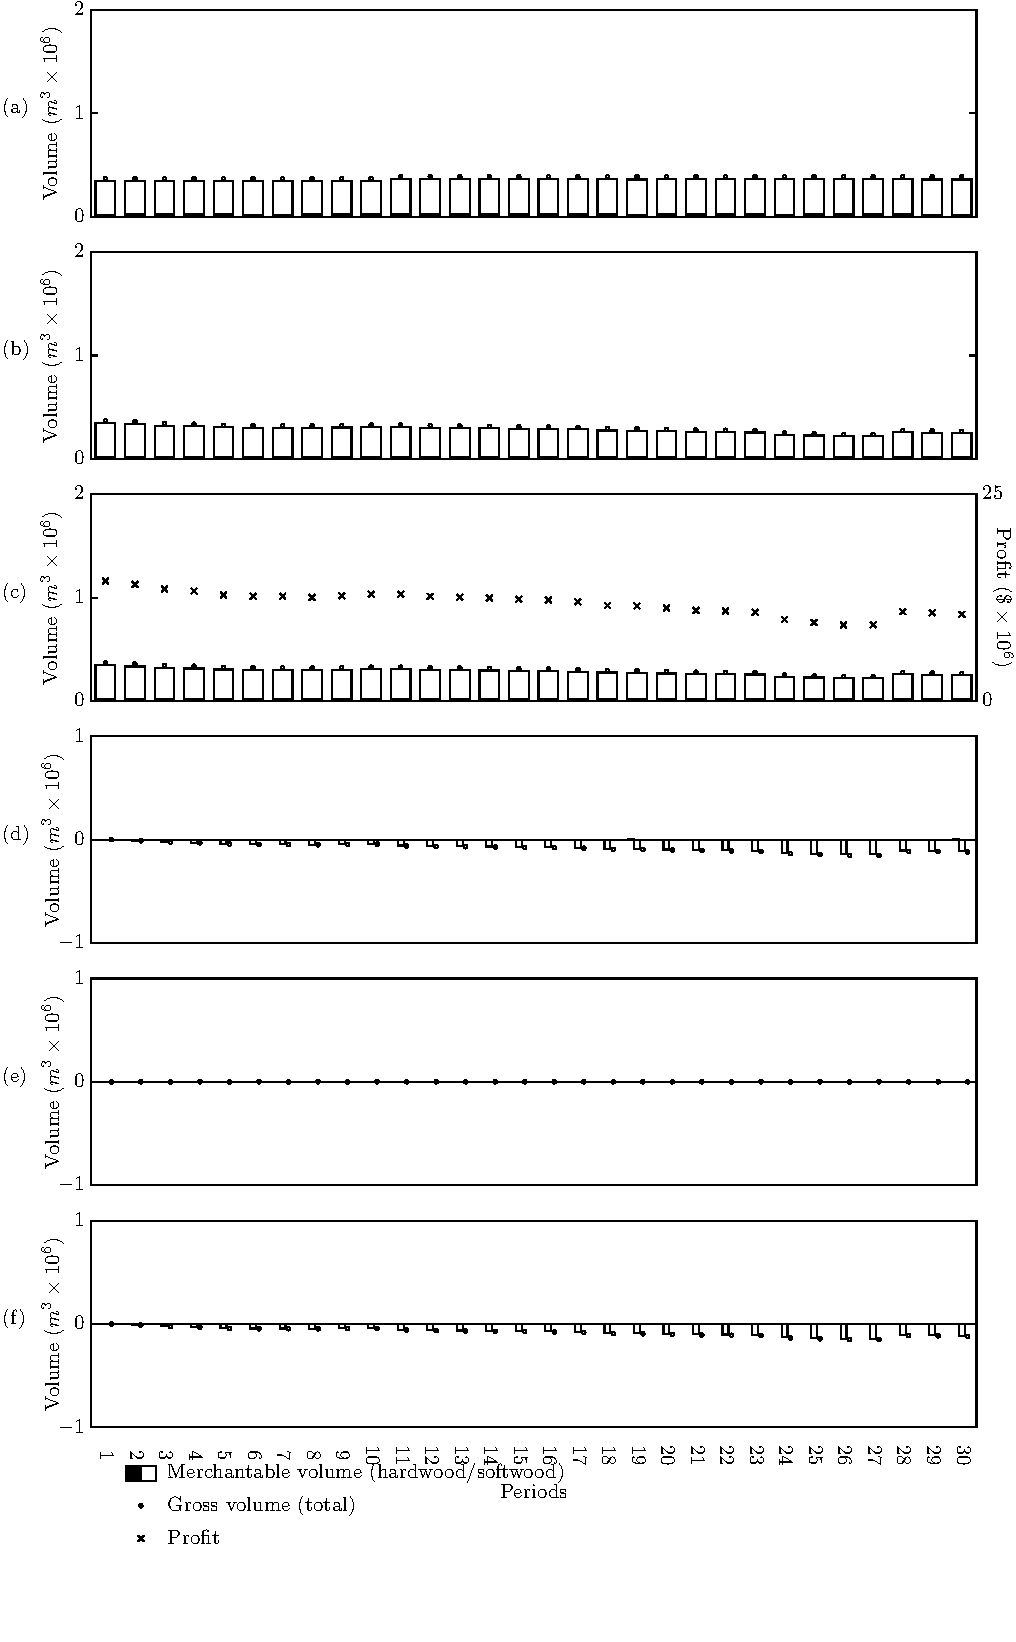
\includegraphics[width=10cm]{images/appendix/s6-1_p30a01}
%   \caption{Base bilevel scenario (same as Scenario 1 presented in Chapter 2).}
%   \label{fig:scenario_bilevel-base}
% \end{figure}

% Some series contain a large number of scenarios. In some cases we present only summary results here, with more detailed simulation results relegated to appendix. Table \ref{tab:scenario_series} summarizes scenario series, with references to appendices.

% \begin{table}
%   \centering
%   \begin{tabular}{lll}
%     \hline
%     Scenario Series Description & Section Reference & Appendix Reference \\
%     \hline
%     Relaxation of line-wise profitability constraint & \S\ref{sec:scenario_series_0} & Appendix \ref{ap:scenario_series_0} \\
%     Varying planning horizon length & \S\ref{sec:scenario_series_0} & Appendix \ref{ap:scenario_series_1} \\
%     %2 & Varying end-product prices & \S\ref{sec:scenario_series_2} & Appendix \ref{ap:scenario_series_2} \\
%     %3 & Varying end-product prices & \S\ref{sec:scenario_series_3} & Appendix \ref{ap:scenario_series_3} \\
%     Varying softwood AAC attribution & \S\ref{sec:scenario_series_4} & Appendix \ref{ap:scenario_series_4} \\
%     Varying tightness of even-flow constraints & \S\ref{sec:scenario_series_5} & Appendix \ref{ap:scenario_series_5} \\
%     \hline
%   \end{tabular}
%   \caption{Description of scenarios in series 6-4.}
%   \label{tab:scenario_series}
% \end{table}

\section{Varying Softwood AAC Attribution}
\label{sec:scenario_series_4}

This scenario series tests the effect of varying the proportion of softwood AAC that the principal attributes to the agent in each planning cycle. This series has a direct potential application to real-world cases; the principal controls the wood supply, and is not obligated to allocate 100\% AAC to timber licencees\footnote{For example, provincial governments policy on Crown forest in Canada typically holds back a small fraction of AAC (around 5\%) with generally vague justification that this hold-back policy satisfies the need for some form of safety buffer in the wood supply.}.

We use a shorthand notation to refer to particular scenarios (e.g., \emph{hw100sw110} refers to the scenario with 100\% of hardwood AAC allocated and 110\% of softwood AAC allocated).
Scenario hw100sw100 corresponds to our reference scenario (i.e., 100\% attribution of both hardwood and softwood AAC). 
We simulate six alternate AAC allocation levels (110\%, 105\%, 95\%, 90\%, 80\%, 60\%. 

As might be expected based on results presented in Chapter 1, over-allocating softwood AAC (i.e., scenarios hw100sw110 and hw100sw105) has a negative effect on long-term wood supply, with wood supply stability deteriorating as a function of over-allocation. However, the effect is moderate; we can conclude the bilevel wood supply model is moderately sensitive to AAC allocation level for our test case. 

Wood supply stabilility improves gradually as we continue to reduce allocation down to 60\% of softwood AAC. At the 60\% allocation level, wood supply stability is completely restored. Withholding a large fraction of softwood AAC indirectly creates a form of safety stock, which offsets gradual wood supply decline observed in the reference scenario\footnote{As discussed in Chapter 2, the slow decline in AAC observed in the reference scenario is attributable to the agent planning his own harvest schedule in the second stage of each planning cycle, which results in a slightly different mix of stand types than those featured in the first period of the optimal wood supply solution. The (deterministic) optimal wood supply solution, being located in an extreme point of feasible solution space, is highly prone to infeasibility, and sensitive to deviations from the optimal solution.}. 

\begin{figure}[H]
  \centering
  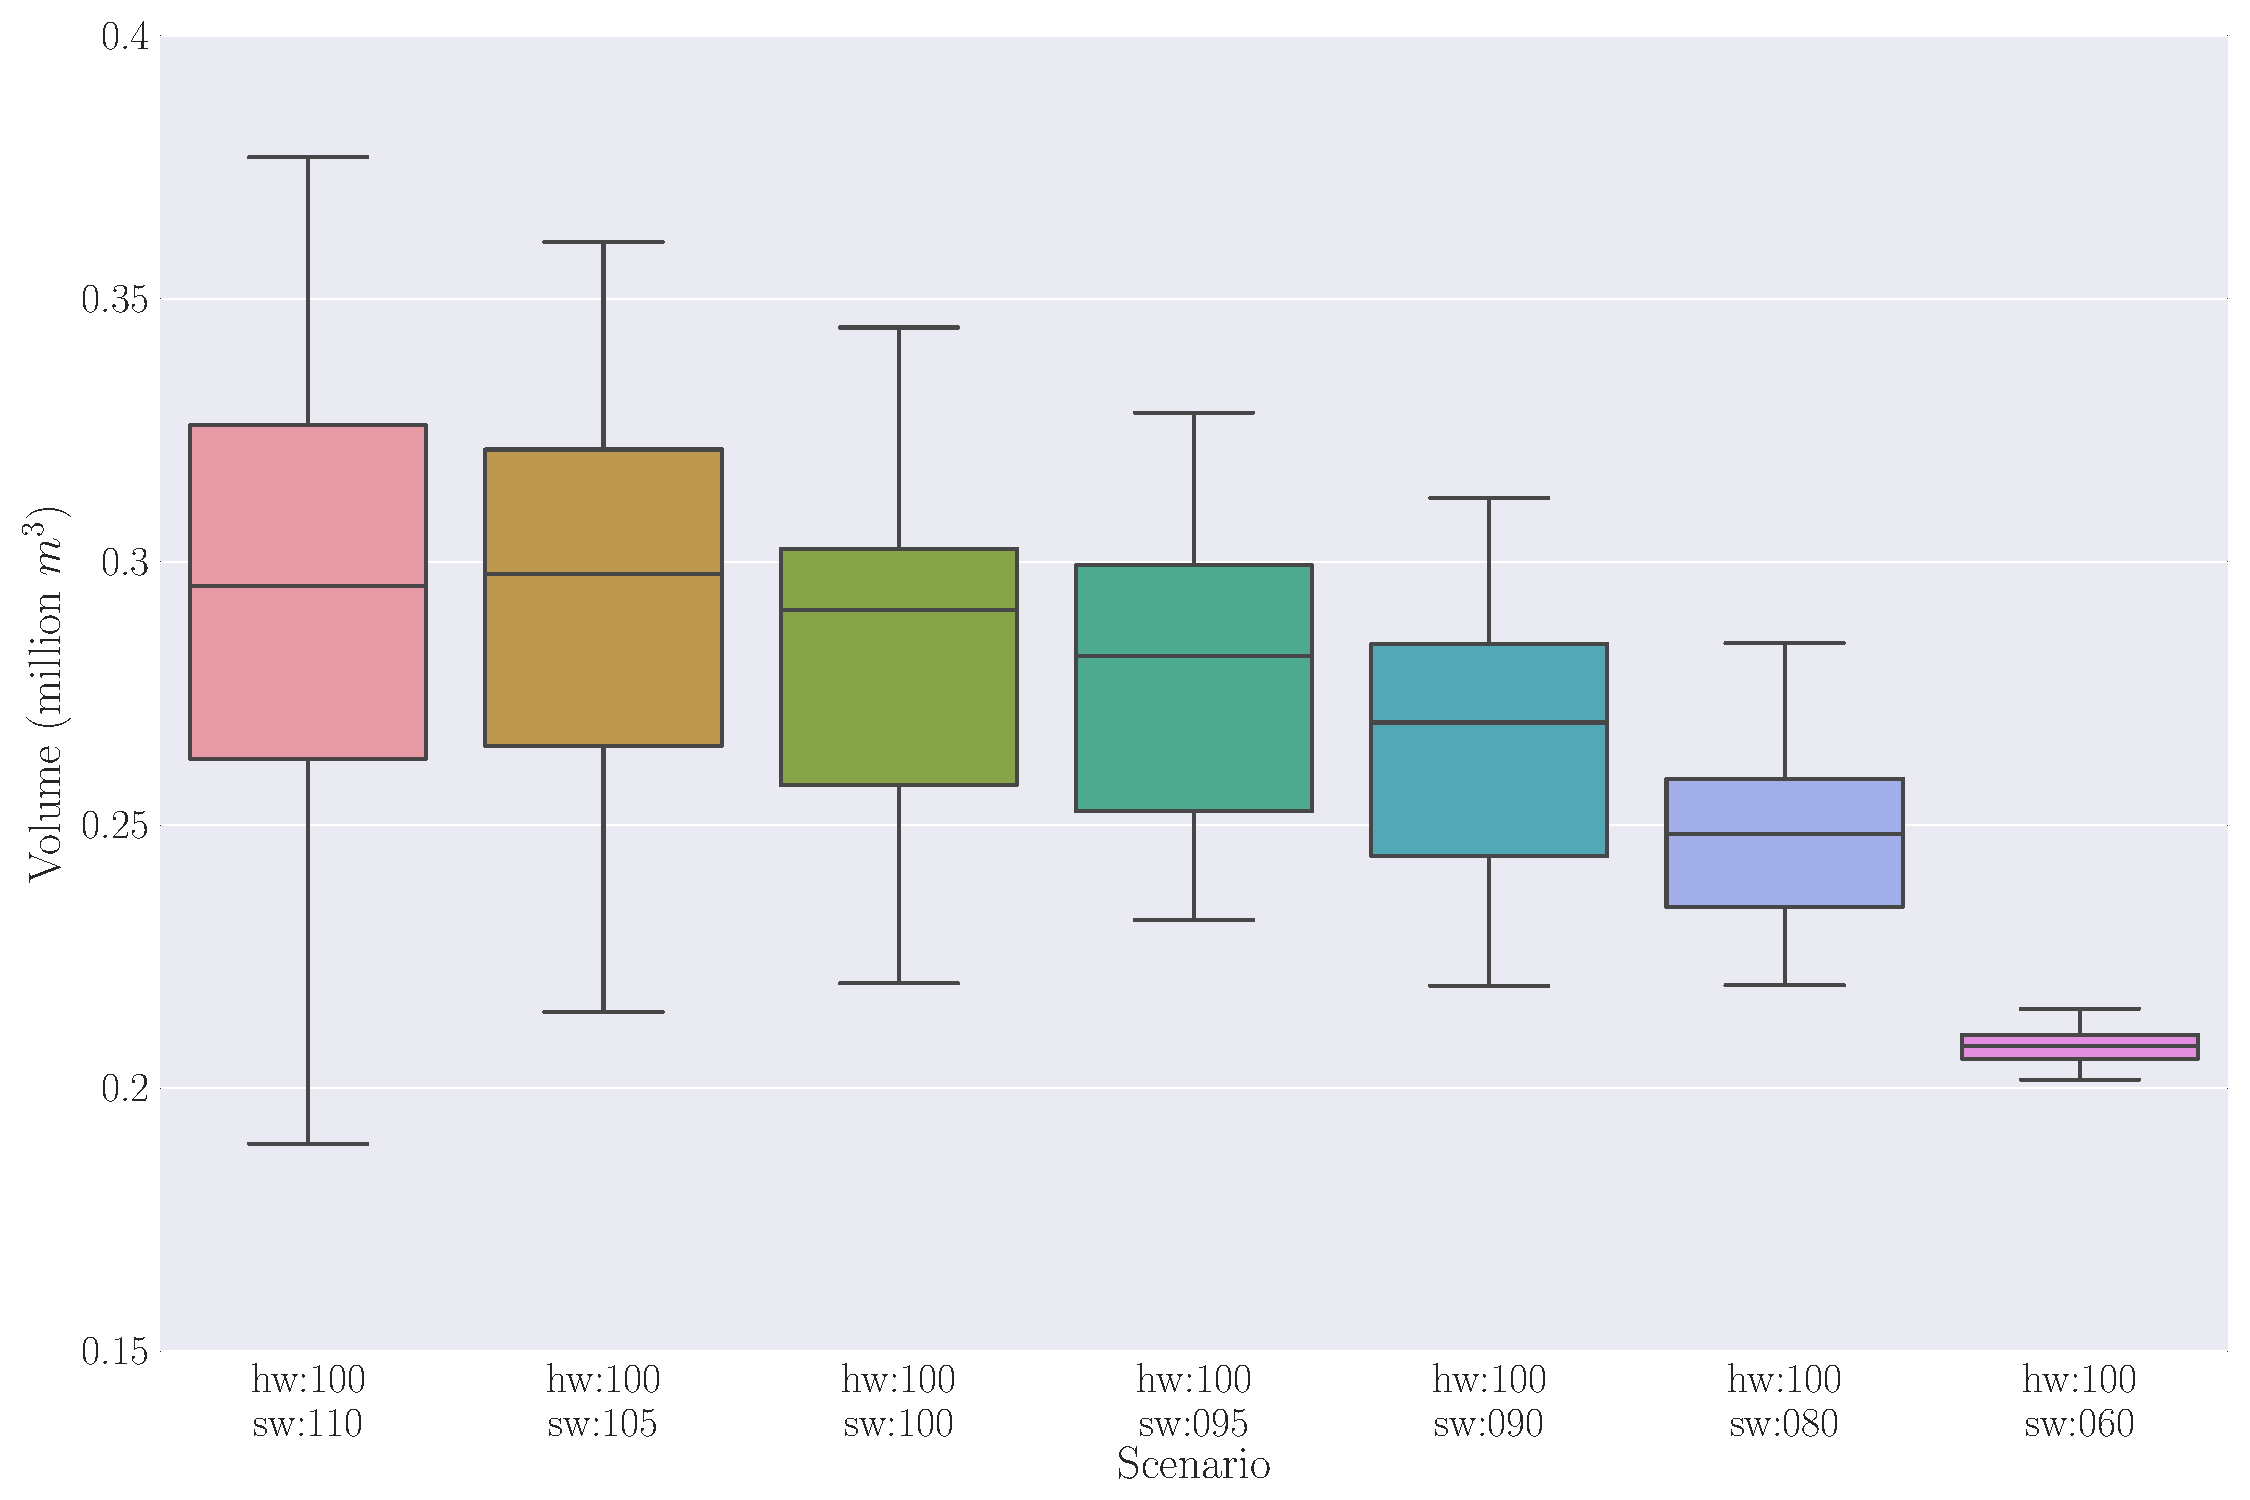
\includegraphics[height=10cm]{images/boxplots_series4}
  \caption{Wood supply stability for a range of softwood AAC attribution levels. }
  \label{fig:scenario_series_4}
\end{figure}

\section{Varying Planning Horizon Length}
\label{sec:scenario_series_1}

This scenario series tests the impact of varying planning horizon length for both principal and agent. 
We test all combinations of horizon lengths for values 30, 20, 10, 5,  and 1 periods. 
Agent horizon is never allowed to be longer than principal horizon, which leaves 15 valid horizon length combinations.
We use a shorthand notation to refer to particular scenarios (e.g., \emph{p30a01} refers to the scenario with a 30-period principal horizon and a 1-period agent horizon).
Scenario p30a01 is our reference scenario for this series, and corresponds to the \emph{status quo} horizon lengths used in Quebec today.
Simulation results reveal interesting patterns on two levels.

%Detailed simulation results are presented in Appendix \ref{ap:scenario_series_1}.

On the first level, longer planning horizons improve stability of long-term wood supply. This effect is most pronounced when comparing scenarios with matched principal and agent horizon lengths (i.e., scenarios p30a30, p20a20, p10a10, p05a05, p01a01). This supports the common belief that long modelling horizons help stabilise solutions from long-term wood supply models (although we use a bilevel wood supply model here, which is not common practice).

One the second level, relative effect of principal horizon length on wood supply stability becomes gradually less pronounced as agent horizon shortens, with the least effect observed for single-period agent horizons. For example, shortening principal horizon length in the reference scenario from 30 to 10 periods (i.e., scenarios p30a01, p20a01, p10a01), has relatively little impact on wood supply. This would indicate that the destabilising effect of short agent planning horizon (due to residual systematic drift that is not anticipated by the bilevel model) overwhelms the stabilising effect of lengthening principal horizon. 

If one focuses on the p30 scenarios (i.e., p30a01, p30a05, p30a10, p30a20, p30a30), results provide some insight into the opportunity cost (in terms of both the magnitude and stability of long-term fibre supply) of maintaining the \emph{status quo} distributed wood supply planning process, where a relatively short-sighted agent is responsible for final implementation of harvesting operations. 

There is a parallel here with the \emph{price of anarchy} concept in game theory \citep{shoham2009multiagent, nisan2007algorithmic}. The contrast between reference scenario p30a01 and best-case scenario p30a30 can be interpreted as an upper-bound estimate of the price of maintaining the \emph{distributed} nature of the wood supply planning process (i.e., allowing the agent to plan his own harvesting, relative to a scenario where the principal controls both long-term wood supply planning and short-term fibre procurement planning processes). 

We specify that this is an \emph{upper bound} estimate, as scenario p30a30 makes rather optimistic assumptions regarding the ability of the principal to produce long- and short-term feasible fibre procurement plans using a simple two-stage planning process as simulated here. Recall that we present simulation results from highly aggregated models. In practice, as-implemented fibre procurement plans are the end product of a complex hierarchical planning process, which iteratively refines plans until they are operationally feasible. Much of the detailed information required to efficiently produce feasible fibre procurement plans is absent from the high-level simulations we present here. To preserve both long- and short-term feasibility, the two-stage planning process (as simulated here) would have to be extended to include an \emph{iterative} dimension; the long-term plan would have to be iteratively constrained, based on feasibility feedback from the (disaggregated) short-term planning level, until the first period of the long-term plan converges with the short-term plan. The process of iterativly constraining the long-term wood supply plan would have either a null (best-case) or negative effect on final AAC, hence our qualification of the contrast between scenarios p30a30 and p30a01 as an \emph{upper bound} estimate of the price of distributed wood supply planning.

In practice, the agent (i.e., the industrial fibre consumer) has both the motivation and the technical expertise required to plan and implement economically efficient short-term fibre procurement plans. It is not clear that the principal has either the proper motivation or the technical capability (recall the information assymmetry that induces the principal-agent problem in the first place) to take over short-term fibre procurement planning (i.e., become an industrial fibre supplier, rather than simply a steward of the public forest resource) without negatively affecting industrial profitability (i.e., stability of fibre cost and value-creation potential). Given the tight profit margins typical of the forest products industry in many jurisdictions, it seems unlikely that the principal could completely exclude the agent from the fibre procurement planning process without destabilising economic sustainability of the forest industry.

Simulation results suggest that the principal could improve long-term wood supply stability by inciting the agent to adopt a longer planning horizon. The case where principal and agent horizon lengths are equal is equivalent to the principal subsuming the agent (i.e., principal has total control of fibre procurement activities, including final selection of stands to be harvested). Note that we simulate perfect anticipation of agent behaviour, thus our simulations results represent optimistic upper bounds potential wood supply. In reality, the principal has limited power to incite the agent to extend his planning horizon beyond one period, so forcing an extension of the agent's planning horizon in the bilevel anticipation may in fact introduce a problematic bias. Development of such incentive policies, using game-theoretic analysis of the decoupling point between principal and agent and the \emph{price of anarchy} concept, represents an interesting direction for futher research.

Note that computational effort required to solve wood supply models can increase exponentially with the number of planning periods for certain model formulations, mostly due to combinatorial explosion of potential future system states for large numbers of planning periods. Our test wood supply model solves very quickly (i.e., approximately 10 seconds), in part due to the efficient SilviLab solver engine, however production models using commercial wood supply modelling software (e.g., Remsoft Woodstock) may require significantly more computational effort to solve similarly-size instances. These long solution times may limit the number of scenarios that can realistically be run by government wood supply analysts, which may in turn limit the quality and scope of wood supply analyses. Our simulation results hint at a potentially interesting tradeoff between computational effort and solution quality. For our test case, principal planning horizon can be shortened by a factor of 3 (i.e., from 30 to 10 periods) with minimal effect on wood supply stability\footnote{We suspect that the amount of planning horizon compression that the principal can safely implement, without inducing unacceptable increase in risk of wood supply failure, is linked to a number of factors that will vary between problem instances (e.g., timing of the critical period and, tightness of even-flow-constraints, etc.).}. Exploratory wood supply scenarios, or sensitivity analyses requiring large numbers of simulations, could potentially be run using shortened model horizons; assuming limited budget for wood supply analysis resources, there is potential to either reduce the cost of analysis with minimal impact on quality, or to improve the quality of the analysis at similar cost.  

%The second pattern is that long-term wood supply is more stable when principal and agent planning horizon lengths are equal. It is not realistic to expect the agent to spontaneously abandon his 1-period horizon in favour of a 30-period planning horizon. However, our simulation results suggest that the principal could indirectly improve long-term wood supply stability by inciting the agent to adopt a longer planning horizon. Although development of such incentive policies is beyone the scope of this project, this represents an interesting direction for futher research.


\begin{figure}[H]
  \centering
  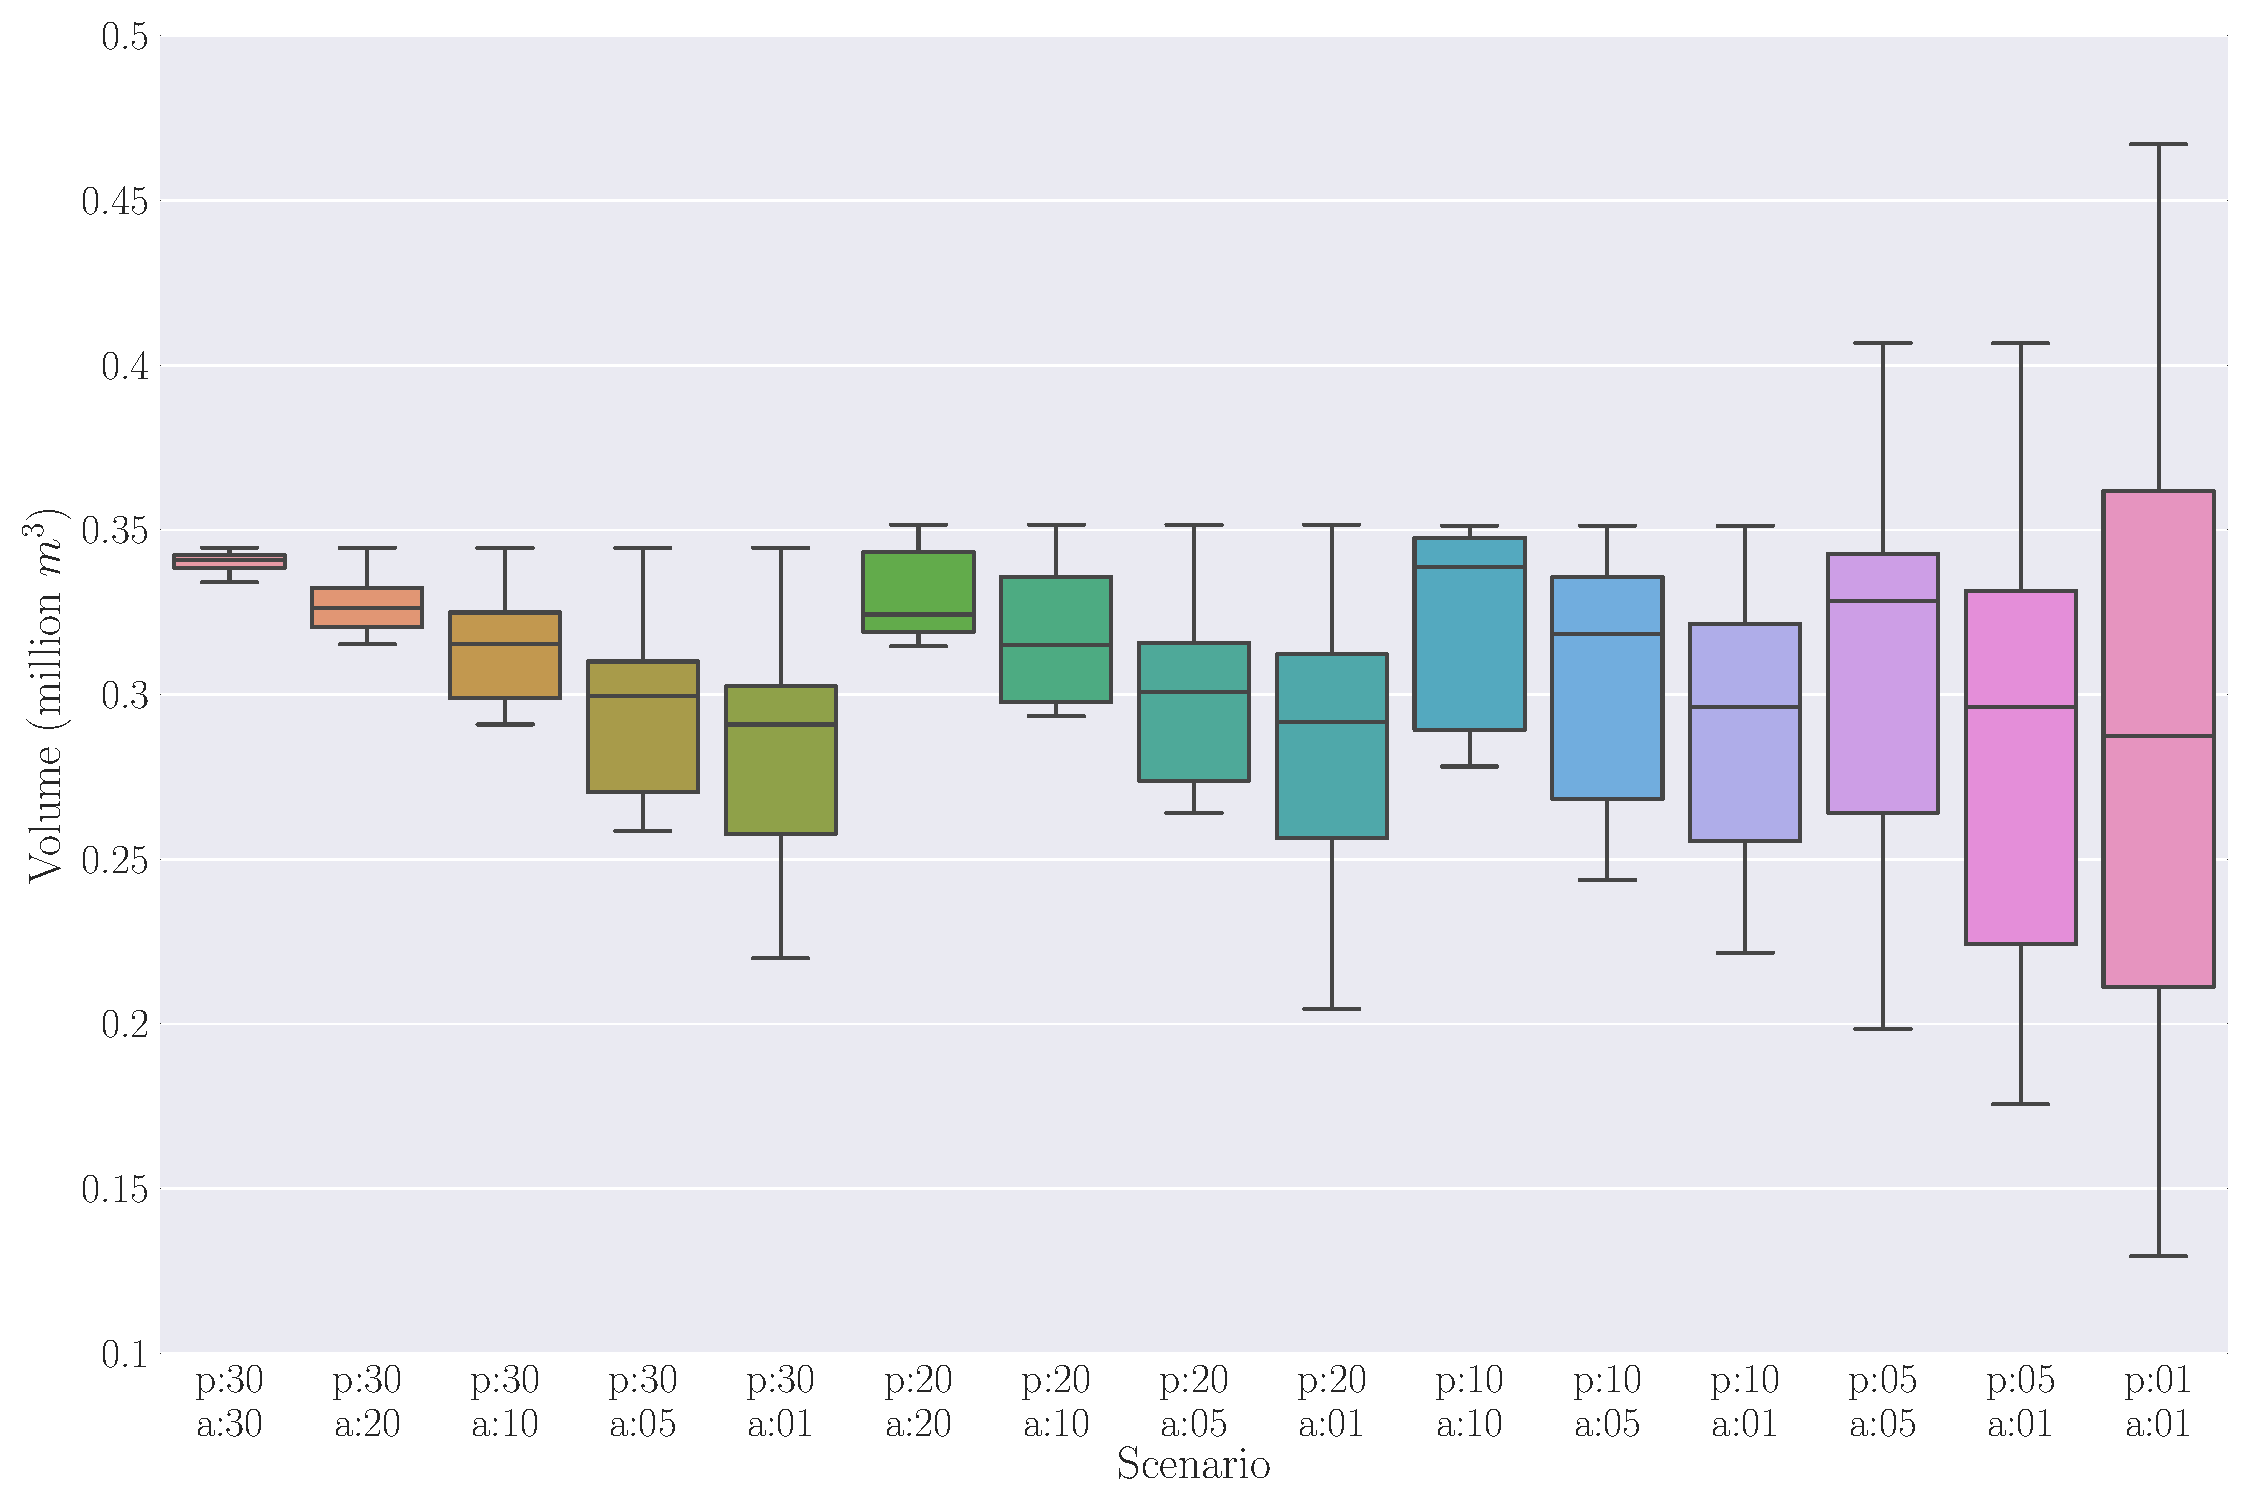
\includegraphics[height=10cm]{images/boxplots_series1}
  \caption{Wood supply stability for a range of combinations of principal and agent planning horizon length. }
  \label{fig:scenario_series_1}
\end{figure}

% \section{Increasing End-product Prices}
% \label{sec:scenario_series_2}

% This scenario series tests the impact of increasing end-product prices in the agent network. We increase all products prices proportionately (i.e., perfectly correlated price increase, relative to reference scenario values), and keep them constant for all 30 iterations. We test ten price scaling factors: 1.6, 2.2, 2.8, 3.4, 4.0, 4.6, 5.3, 5.9, 6.4, and 7.1. 

% We were initially surprised to observe that prices could be scaled by up to 400\% with only negligible effect on agent fibre consumption volume. Further analysis revealed that this is expected behaviour, given the configuration of our test dataset. Low capacity of the single hardwood sawmill is the binding constraint (i.e., bottleneck) for the first five scenarios in this series; the increase in hardwood end-product price is not sufficient to offset the cost of 

% , until prices are scaled by a factor of 4.6, at  which point agent fibre consumption (and profit) increases suddenly 

% \section{Decreasing End-product Prices}
% \label{sec:scenario_series_3}


\section{Varying Tightness of Even-flow Constraints}
\label{sec:scenario_series_5}

This scenario series tests the effect of varying the tightness of even-flow constraints. The reference scenario hw005sw005 simulates a 5\% even-flow constraint gap for both hardwood and softwood. We simulate 5 alternate tighness values (0\%, 1\%, 10\%, 20\%, and 50\%). 
We use a shorthand notation to refer to particular scenarios (e.g., \emph{hw001sw001} refers to the scenario with a 1\% even-flow constraint gap for both hardwood and softwood).

As might be expected, long-term wood supply is more stable when the constraints are tighter, and more variable when the constraints are relaxed. Furthermore, relaxing the even-flow constraints has a negative effect on mean AAC. However, our model is relatively insensitive to this parameter, and remains surprisingly stable with a 50\% even-flow constraint gap. 

\begin{figure}[H]
  \centering
  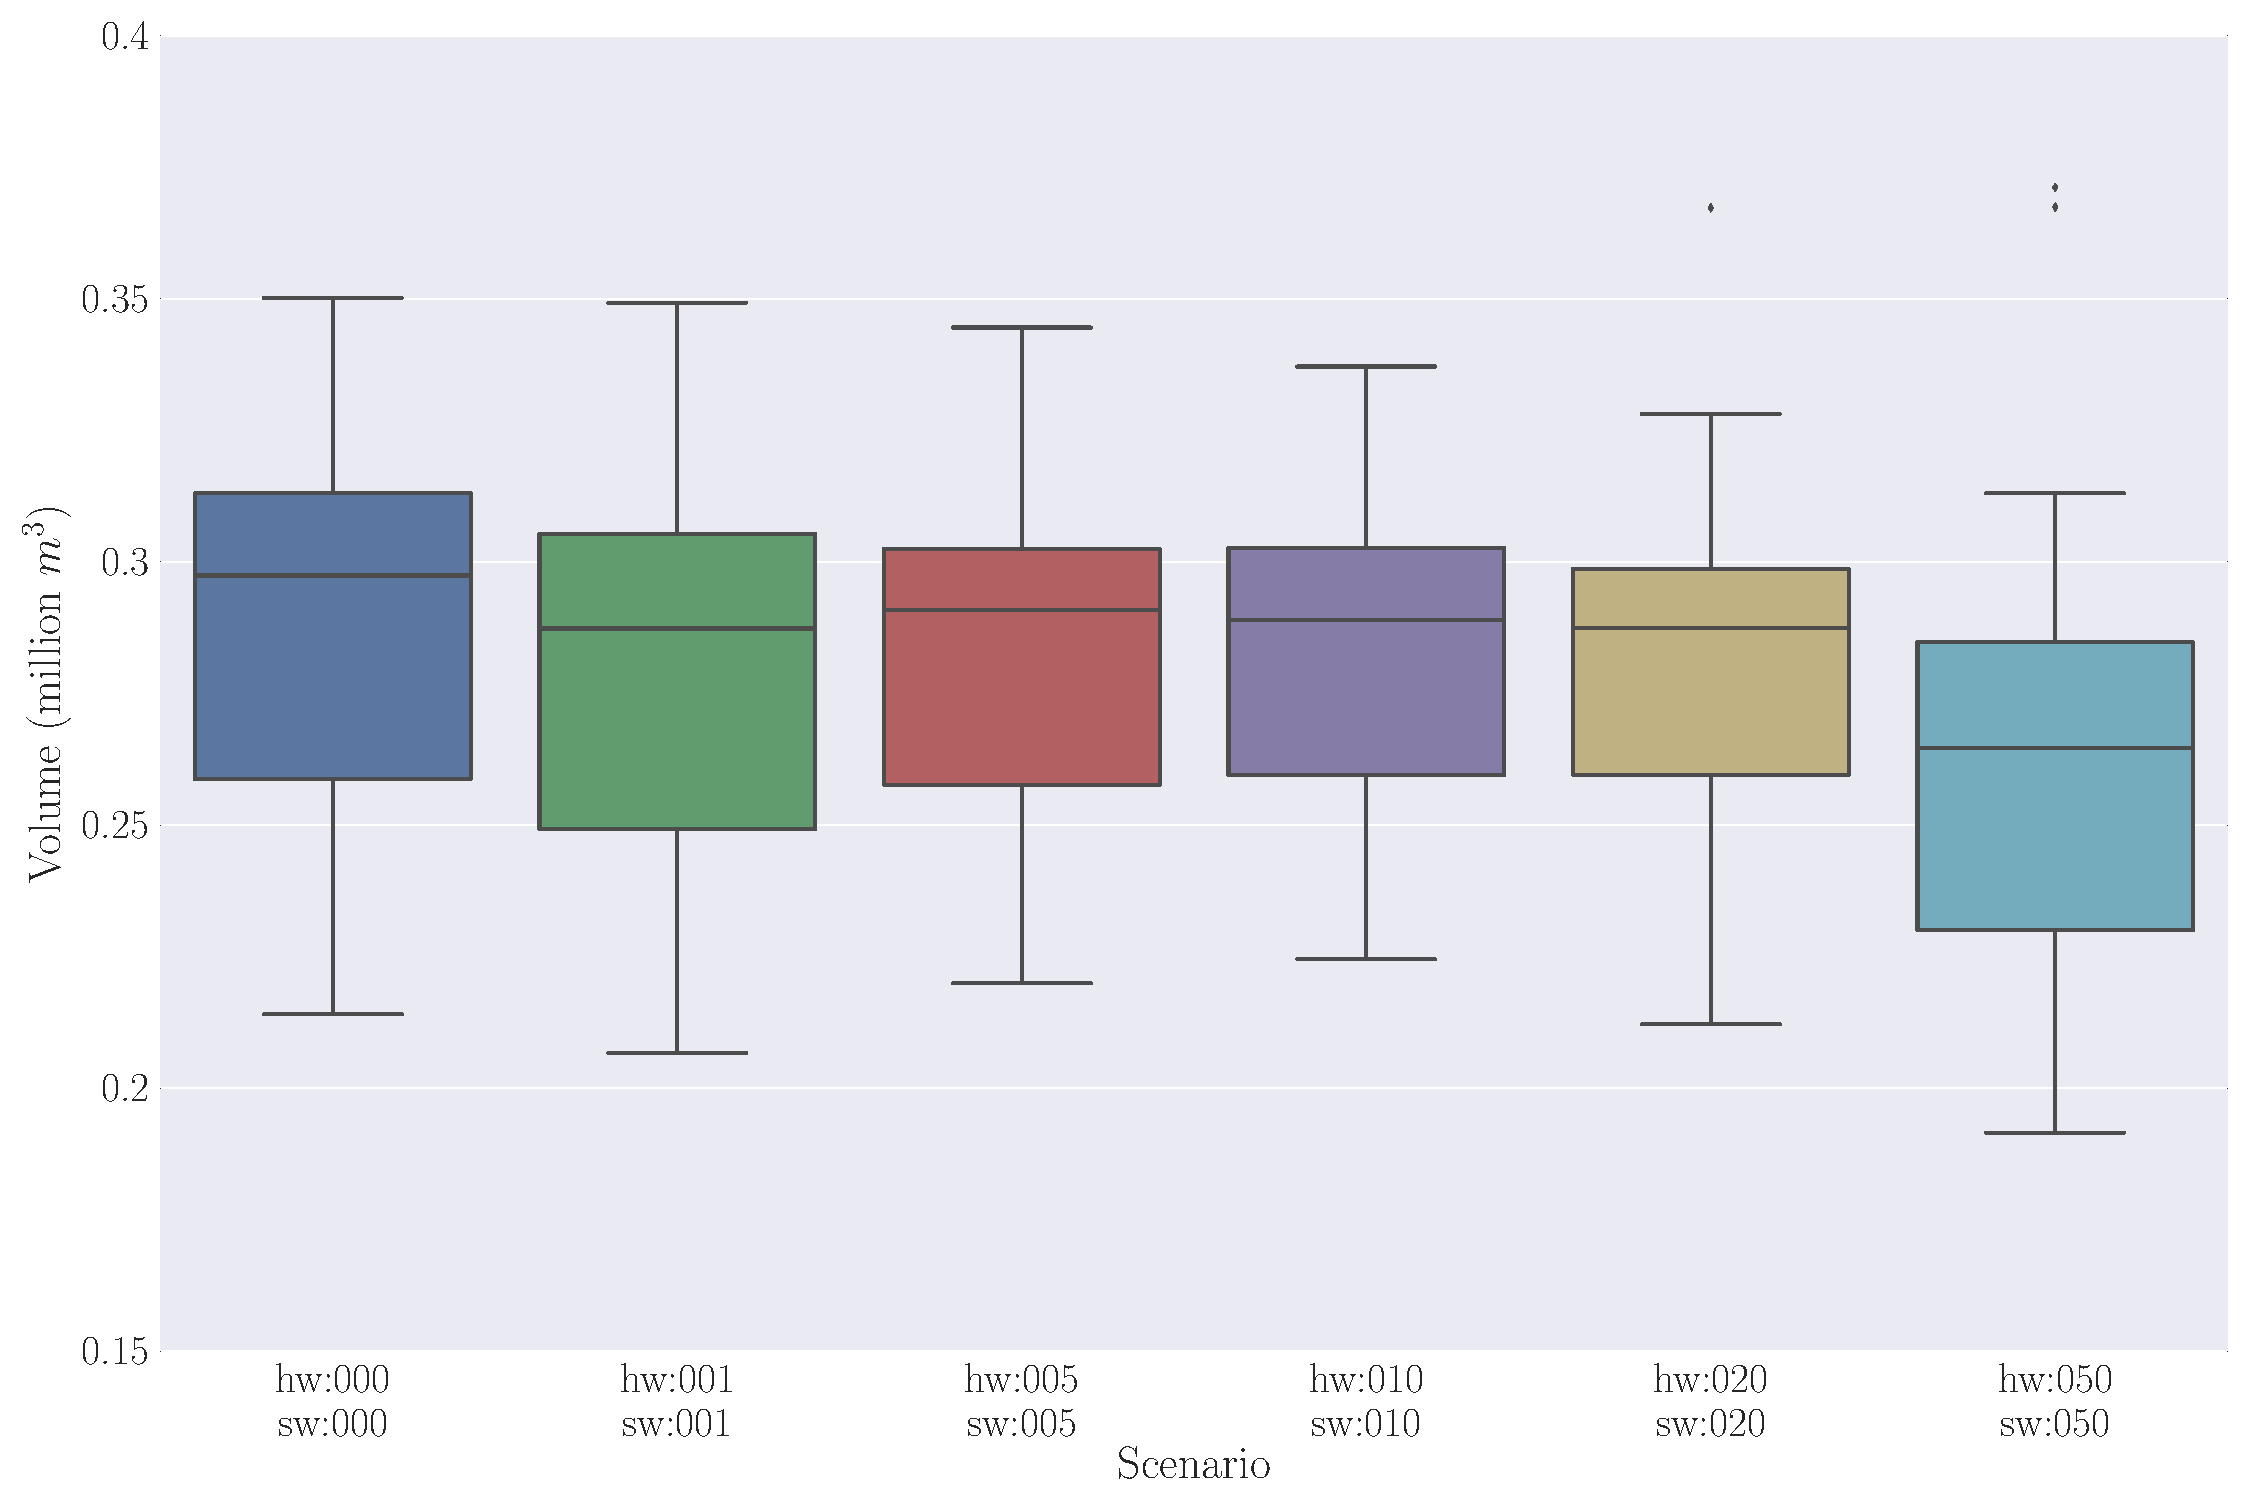
\includegraphics[height=10cm]{images/boxplots_series5}
  \caption{Wood supply stability for a range of even-flow constraint tighness levels. }
  \label{fig:scenario_series_5}
\end{figure}

\section{Stochastic Agent Fibre Demand}
\label{sec:scenario_series_6}

The reference scenario optimistically simulates perfect anticipation of agent fibre consumption volume. In practice, we expect some random error in the principal's anticipation of fibre demand. This scenario series tests the sensitivity of wood supply to controlled stochasticity in actual agent fibre demand.


To implement this scenario series, we simulate randomly-generated AAC consumption levels in the second stage of each planning cycle. More specifically, we randomly generate the proportion of AAC consumed in each cycle by sampling from a uniform distribution on the interval $[0.9, 1.1]$ (i.e., AAC $\pm 10\%$). This is similar to the range and distribution of historic variation in AAC consumption in Canada between 1990 and 2012 (see Figure \ref{fig:aac_consumption}).

Figure \ref{fig:scenario_series_6} presents results from 20 replicates of the experiment, comparing re-planned AAC for the reference (i.e., deterministic) and test (i.e., stochastic) demand scenarios. For the stochastic scenario, we plot the $2\sigma$ error band (i.e., 95\% of expected variability is contained within the error band). 

\begin{figure}[H]
  \centering
  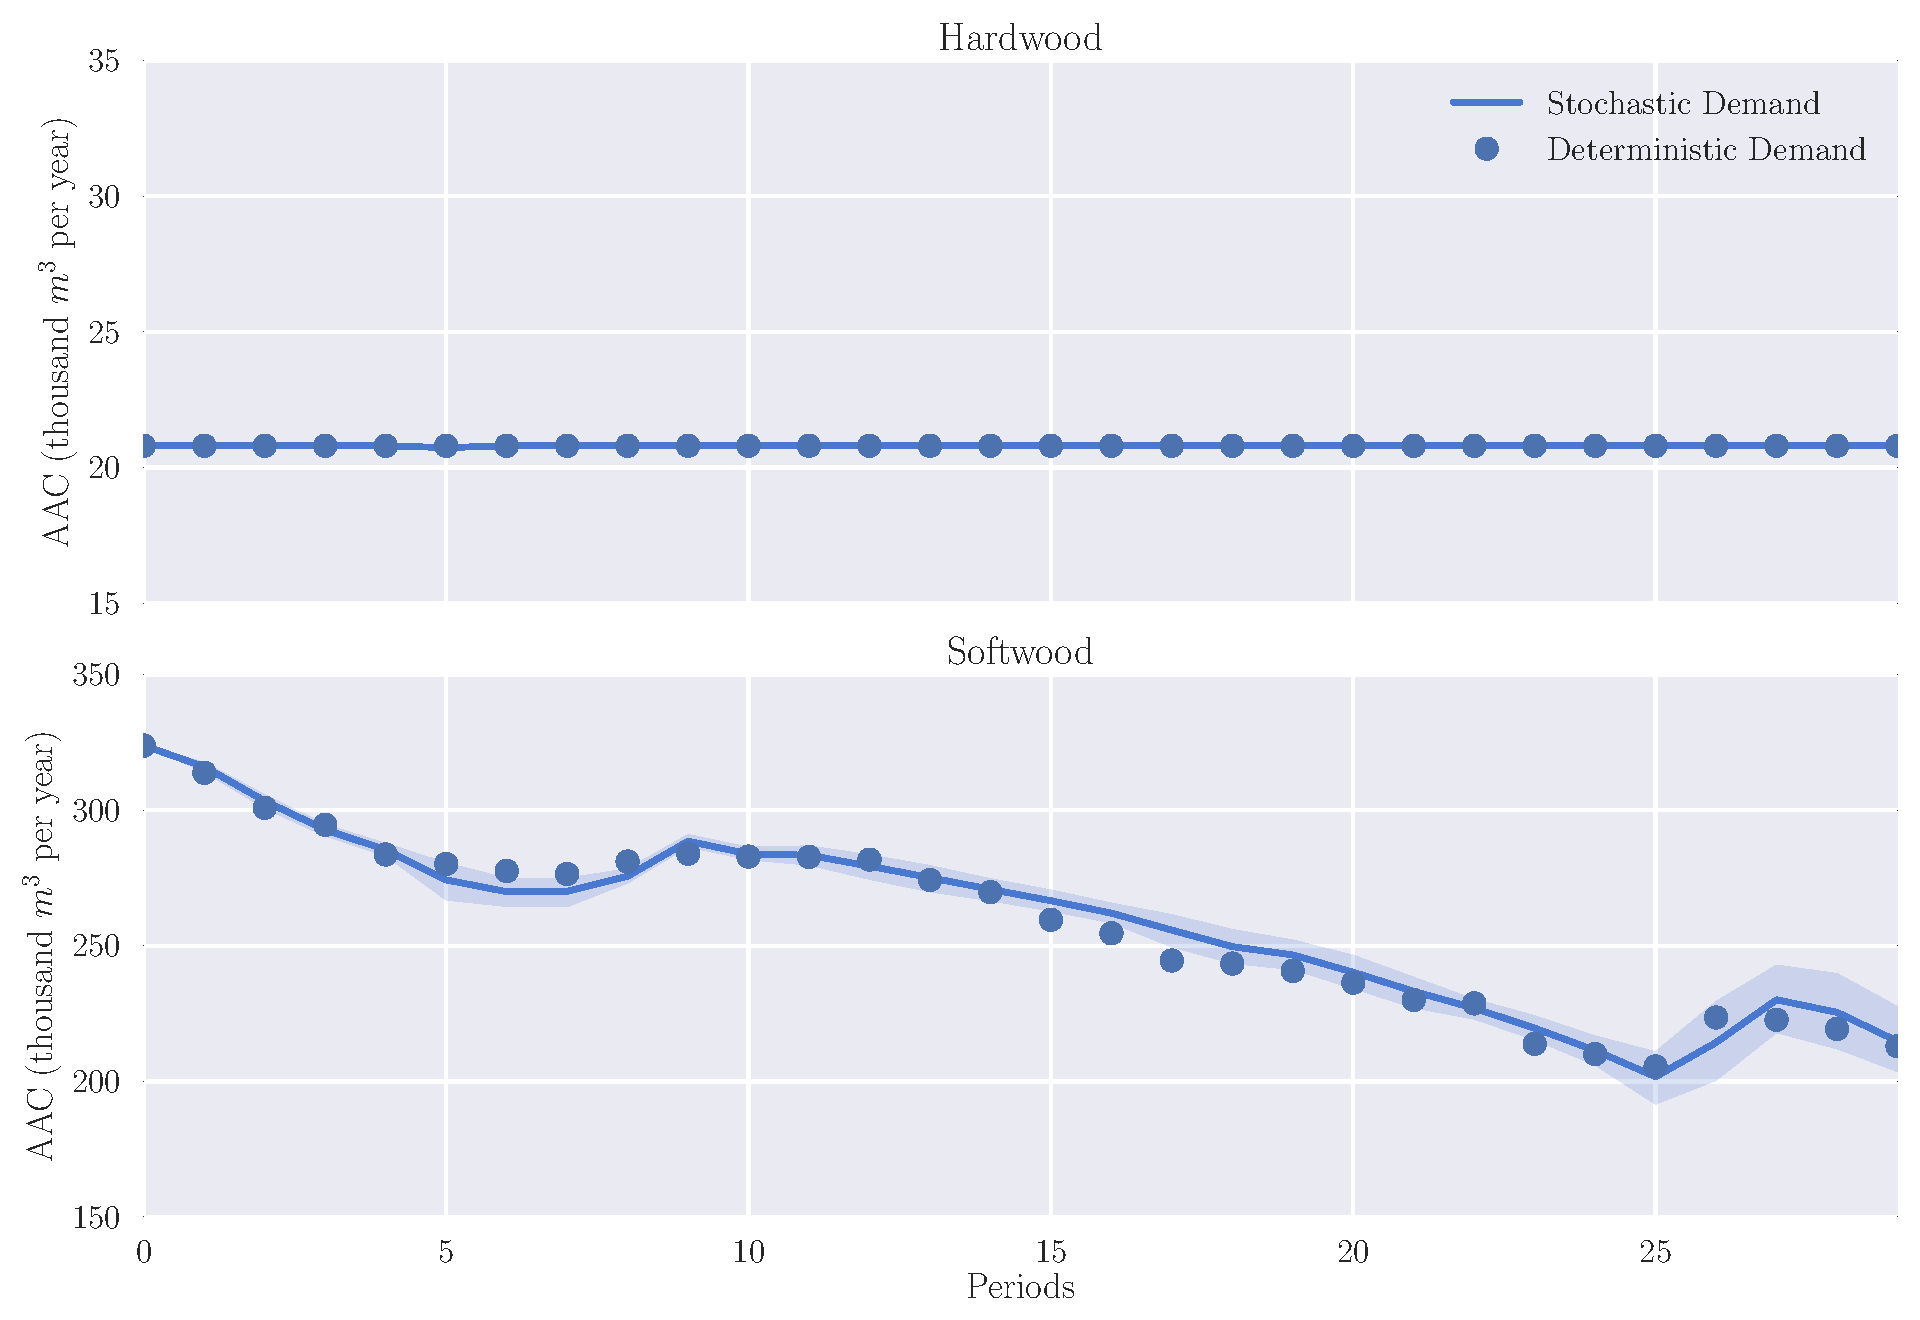
\includegraphics[width=\textwidth]{images/tsplot_2sigma}
  \caption{Comparison of re-planned AAC under deterministic (reference) and stochastic (test) anticipation of AAC consumption.}
  \label{fig:scenario_series_6}
\end{figure}
 
These simulation results show that error in anticipation of demand within the bilevel model is not problematic when actual fibre demand is uniformly distributed on an interval centered on current AAC. This is an important result in terms of potential feasibility of implementing a bilevel wood supply modelling solution in practice; although real-world implementation of the agent-anticipation mechanism will never be perfect (i.e., there will always be residual information asymetry between the principal and the agent), this error many not have a significant effect on long-term wood supply sustainability \emph{as long as it is not biased} (i.e., mean fibre consumption is randomly distributed on an interval centered on AAC).  

These results have an interesting potential policy application. The principal could potentially allow the agent to exceed AAC in periods of peak demand and lag behind AAC in periods of depressed demand. By providing a certain amount of short-term flexibility, this type of policy could potentially allow the agent to improve mean profit, by capturing more short-term value creation opportunities, without compromising sustainability of the wood supply.

\section{Relaxation of Line-wise Profitability Constraint}
\label{sec:scenario_series_0}

%%%%%%%%%%%%%%%%%%%%%%%%%
% Text pasted from article 2:

% Scenario 6 shows the potential benefit of relaxing the agent's line-wise profitability constraint. This simulates a more centralized fibre procurement behaviour in the agent than the standard agent behaviour simulated in scenarios 2 through 5. Scenario 6 allows the agent to maximize the sum of profits from both hardwood and softwood lines. This opens up the possibility for the agent to dispose of excess hardwood fibre supply (at a moderate cost) in order to gain access to significant extra volume of softwood from previously-inaccessible high-hardwood-content mixedwood stands. The cost of disposing of the relatively small volume of excess hardwood fibre is offset by the profits from processing and sale of a relatively large volume of newly-available softwood fibre. 

% This increase in hardwood fibre consumption has a positive-feedback effect on long-term fibre supply; the principal may now harvest the problematic mixedwood stands at a faster in the first few planning cycles. These mixedwood stands (which where left standing in previous scenarios) can now be replaced with pure softwood plantations. In the medium term, this has the effect of partially re-aligning the inventory of standing timber with industrial fibre demand. In practice, agent behaviour more closely resembles the greedy agent bhaviour simulated in scenarios 1 through 6.

% Centralized fibre procurement planning almost double average fibre consumption (92\% increase) relative to scenario 3 (i.e., base bilevel scenario). This significant increase in potential fibre consumption represents an important opportunity of the agent, however implementing intra-agent collaborative fibre procurement behaviour is between the is beyond the control of the principal. There is nonetheless a clear incentive for the principal for lobby the agent to align his fibre consumption capacity with the potential wood supply. 
%%%%%%%%%%%%%%%%%%%%%%%%%%%%%

Our base bilevel scenario imposes a \emph{line-wise profitability} constraint on the agent sub-model. For our test case, we aggregate all fibre flows into the agent model into two product lines (i.e., \emph{hardwood} and \emph{softwood}). The line-wise profitability constraint requires fibre flows from each of these lines to be independently profitable, which  plays an important role in our simulation of wood supply failure in Chapter 1. The line-wise profitability constraint in our agent model reflects a common situation in many real-world value creation networks: hardwood and softwoood mills are independently owned and managed, which affects the species composition of stands that are scheduled for harvest in each planning cycle.  

For our test dataset, hardwood fibre consumption is constrainted by low hardwood fibre processing capacity\footnote{Hardwood logs must pass through a single hardwood sawmill, whose annual processing capacity is limited to approximately one third of initial hardwood AAC.}. Flow conservation constraints in our model limit harvest volume to consumed volume (i.e., all harvested fibre must be consumed). In the reference scenario the combination of low hardwood processing capacity, high softwood fibre demand, line-wise profitability constraints and flow conservation constraints limits sustainable bilevel AAC. 

%To harvest the entire softwood AAC while limiting hardwood fibre harvesting to a fraction of AAC, the stands selected for harvest by the agent (in the second stage of each planning cycle) must feature a higher proportion of softwood than the stands that are schedule for harvest in the first period of the wood supply model solution. The forest stands available for harvesting in future planning cyclces are affected by what was harvested in the current planning cycle. 

%Thus, agent avoidance of hardwood-rich stands in his harvesting plans causes systematic drift of the forest system state: the unharvested hardwood-rich stands form an increasingly large proportion of standing timber inventory. Mature softwood-rich stands grow increasingly scarce at each planning cycle, forcing the agent to reduce his total consumption volume. 

Our test dataset features an alternative agent process that could potentially consume hardwood fibre (besides the single hardwood sawmill), which we will designate the \emph{storage} process. The storage process has a negative net unit value (i.e., the agent has to pay a constant unit cost to push fibre through this process). The line-wise profitability constraints prevent any fibre form flowing through this process in the reference scenario. 

If the line-wise profitability constraints are relaxed in the agent model (i.e., if we simulate centralized agent fibre procurement planning), the cost of pushing fibre through the storage process may be offset by profits from the additional fibre that can be pulled through the softwood line, which in turn would allow the principal to sustainably increase bilevel AAC. 

Figure \ref{fig:scenario_series_0} shows simulation results for a scenario where we relax the line-wise profitability constraints in the agent model.  This simulates perfectly integrated (i.e., collaborative) agent fibre procurement behaviour, and makes it possible for the hardwood line to operate at a net loss if this is profitable for the network as a whole. 

\begin{figure}[H]
  \centering
  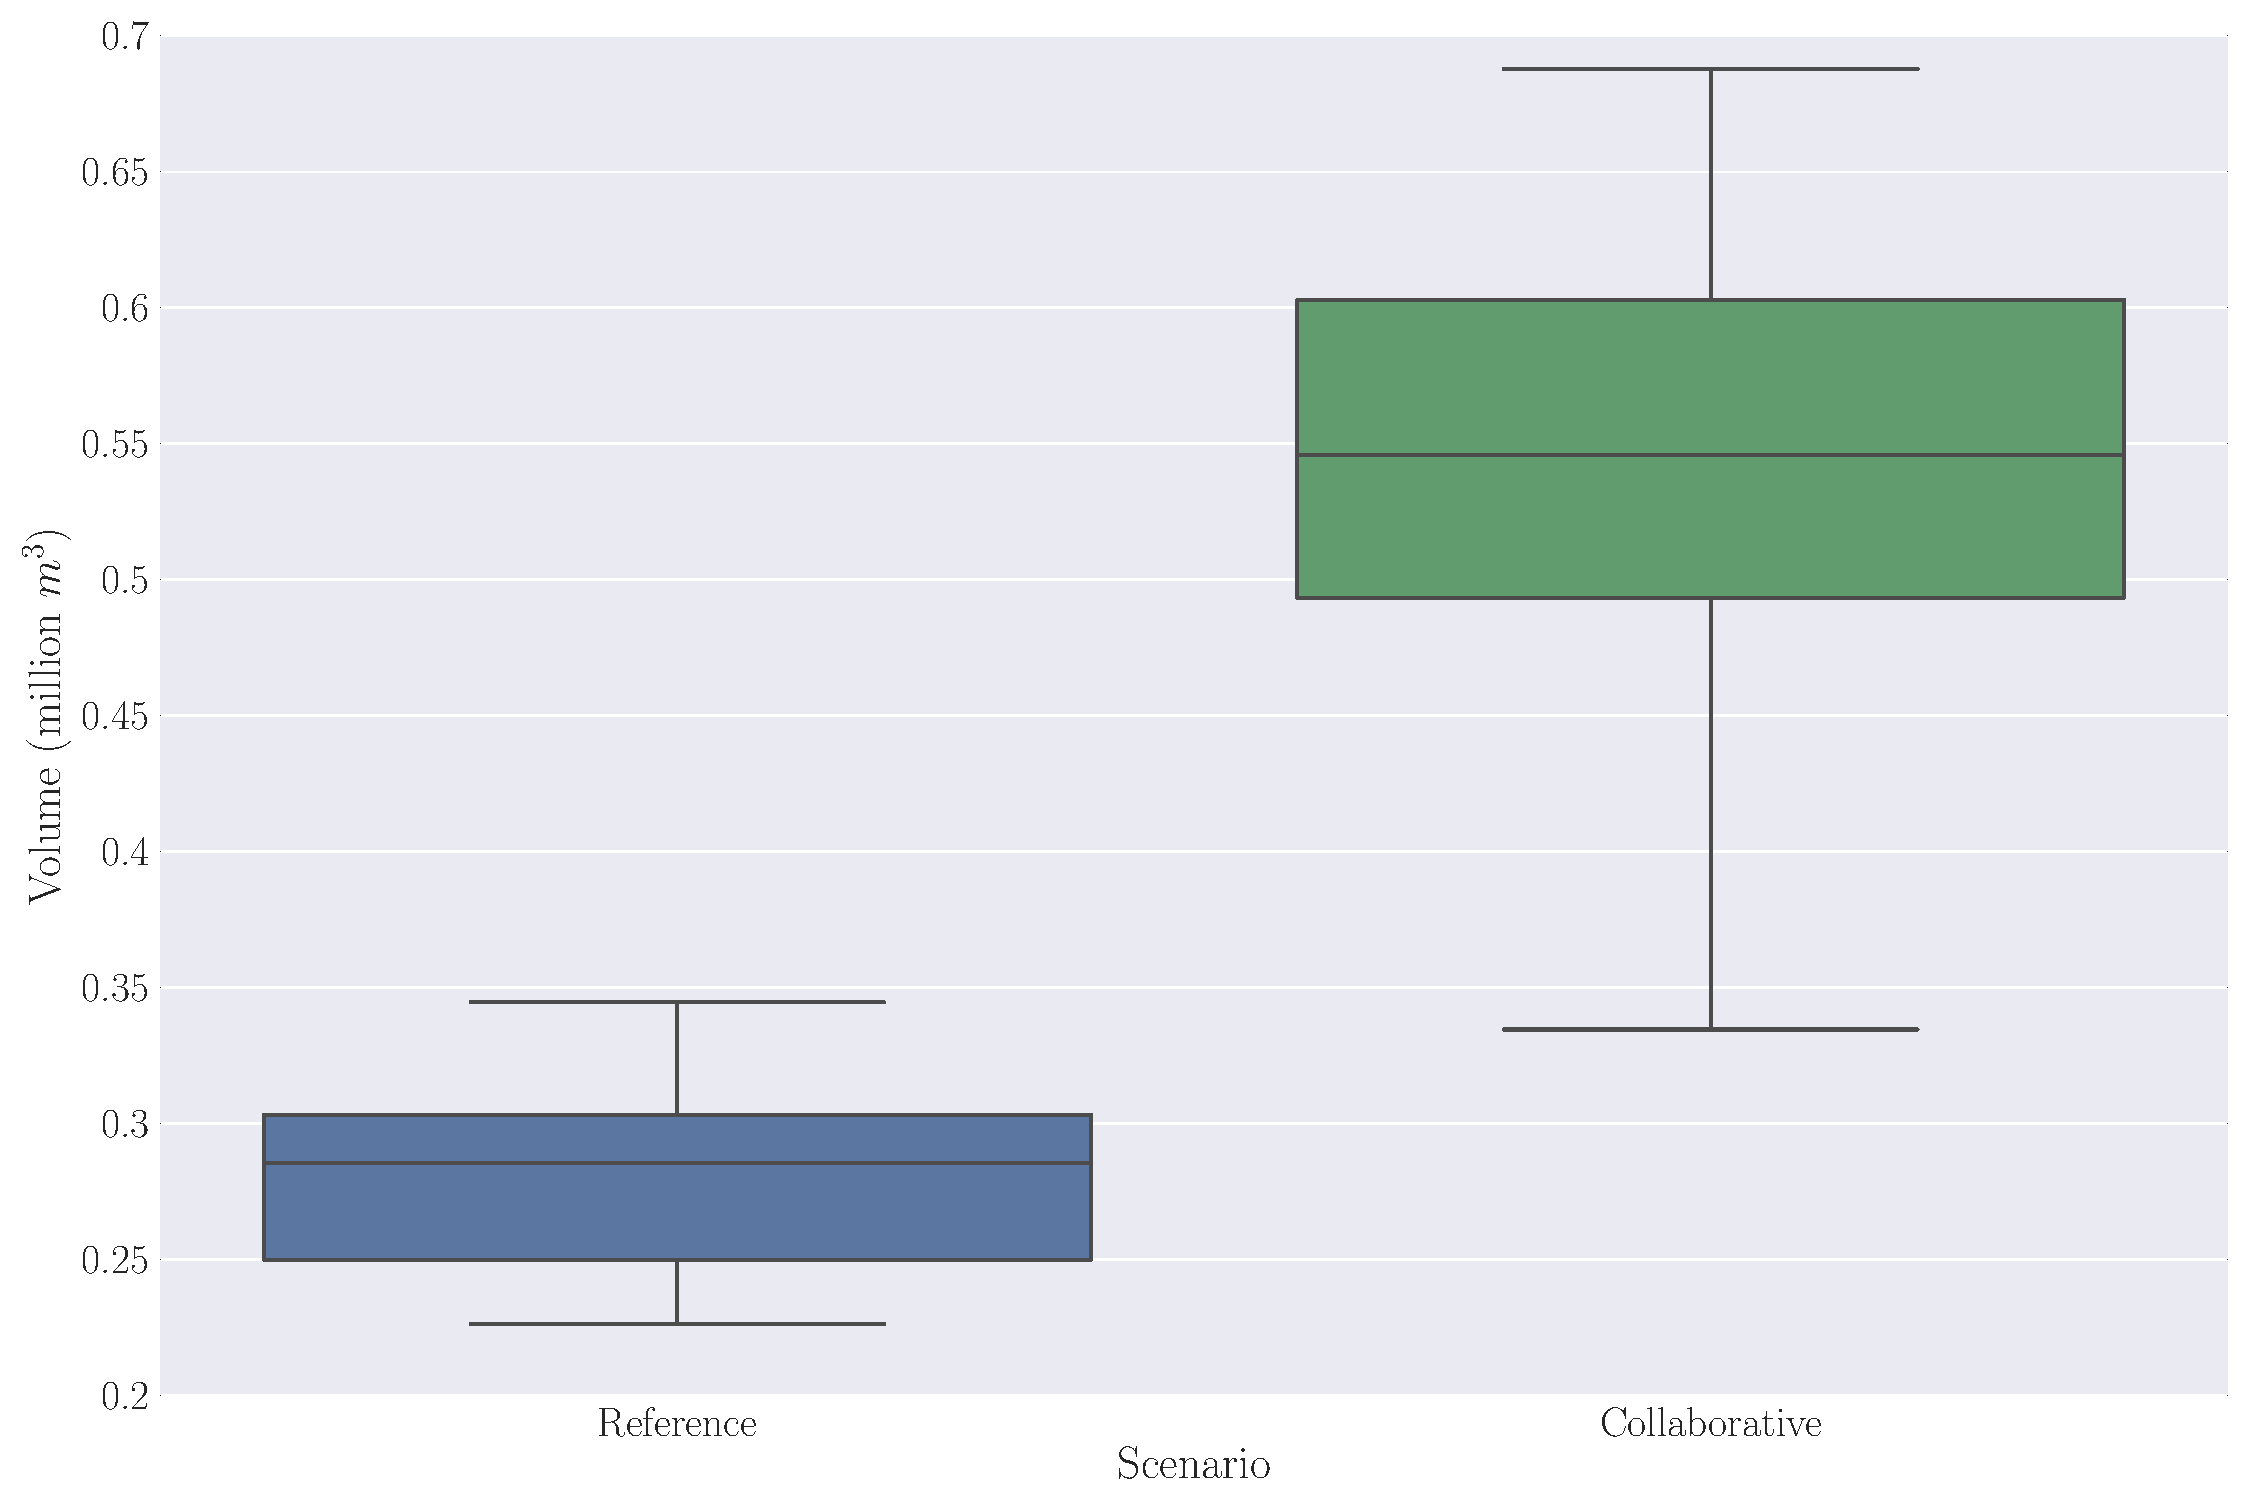
\includegraphics[width=\textwidth]{images/boxplots_series0}
  \caption{Effect of relaxing line-wise profitability constraint (i.e., centralizing agent fibre procurement) on magnitude and stability of wood supply. }
  \label{fig:scenario_series_0}
\end{figure}


% \begin{figure}[h]
%   \centering
%   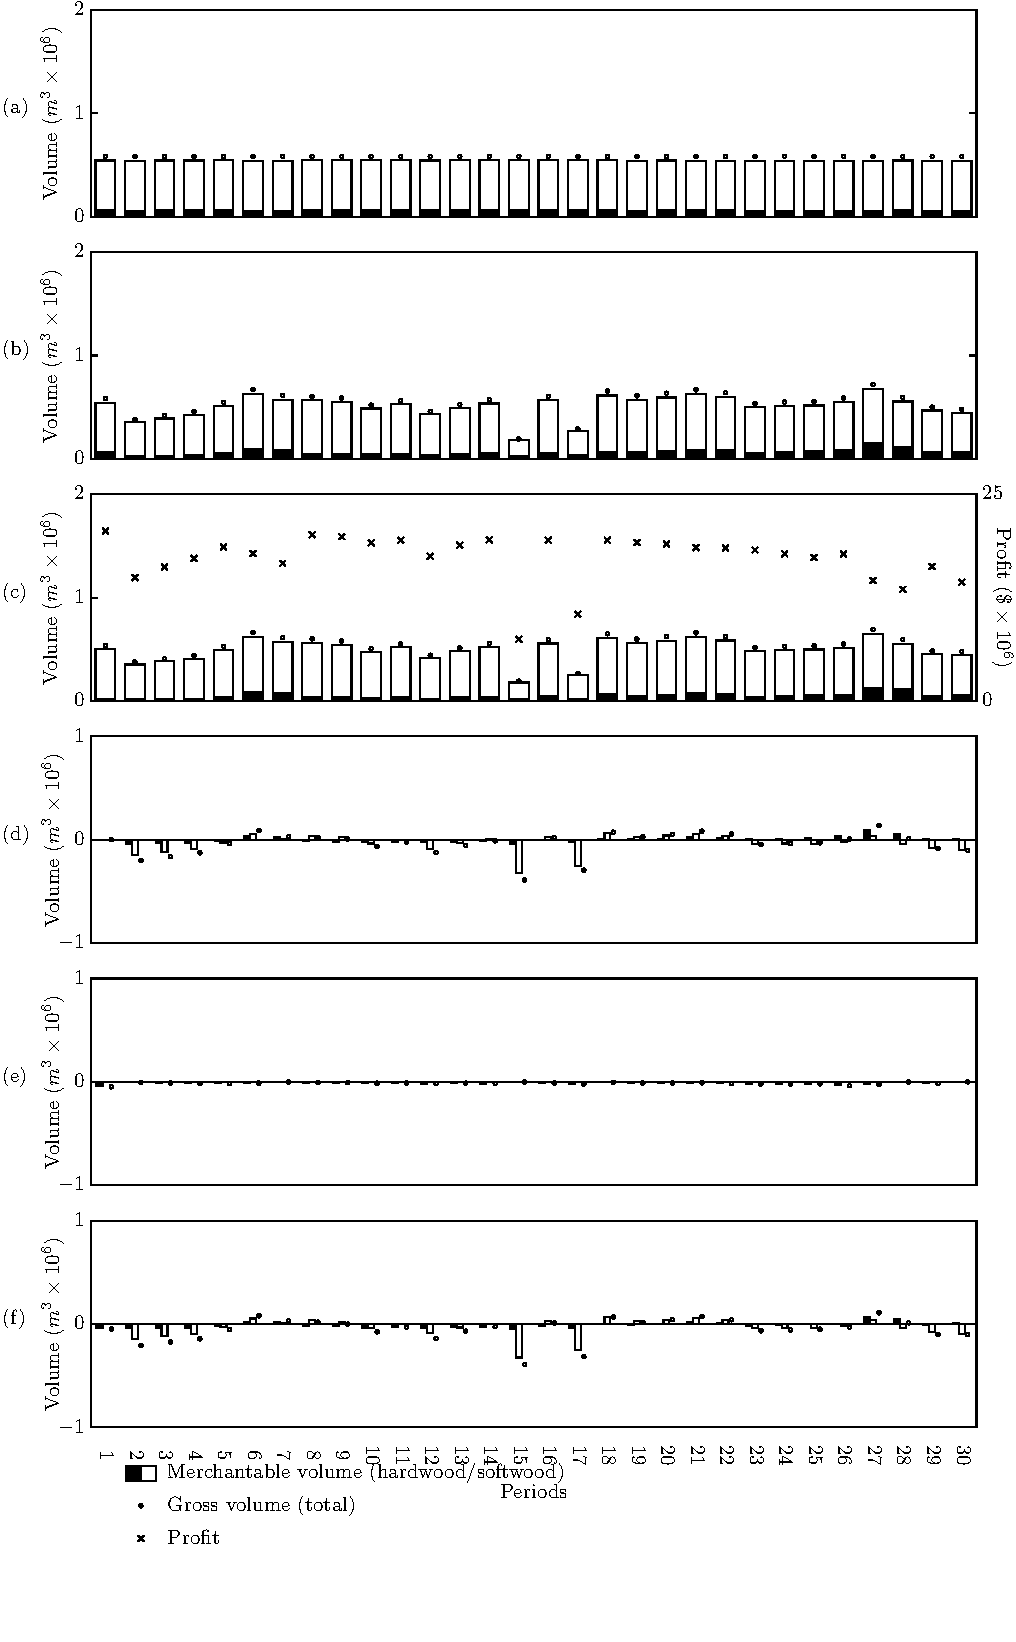
\includegraphics[width=10cm]{images/appendix/s6-6_base}
%   \caption{Scenario simulating relaxed line-wise agent profitability constraint}
%   \label{fig:s6-6_base}
% \end{figure}

\subsection{Benefits and Challenges of Collaborative Fibre Procurement Planning}

Collaborative fibre procurement planning almost double average fibre consumption (92\% increase) relative to the reference scenario. 
%This represents an important opportunity of the agent, however 
Implementing intra-agent collaborative fibre procurement behaviour is beyond direct control of the principal, but he has a clear incentive\footnote{As indicated by the objective function of the wood supply model, which maximizes long-term sustainable fibre consumption.} to lobby the agent to align fibre consumption capacity with potential wood supply. 

For our test case, the increase in hardwood fibre consumption under collaborative fibre procurement planning has a positive-feedback effect on long-term fibre supply. The principal may now harvest the problematic mixedwood stands in the first few planning cycles. These mixedwood stands, which are left standing in the reference scenario, can now be replaced with pure softwood plantations. In the medium term, this has the effect of partially re-aligning the inventory of standing timber with industrial fibre demand. In practice, agent behaviour more closely resembles the greedy agent behaviour simulated in the reference scenario.

The collaborative scenario simulates willingness of the hardwood line to operate at a net loss to benefit the rest of the network.
Some form of collaborative benefit-sharing agreement would have to been in place for this setup to be economically viable for the hardwood sub-agent. Although the potential for collaborative benefit-sharing has been discussed in the litterature, for forestry and other supply-chain contexts \citep{audy2012framework, lehoux2011collaboration, forget2008collaborative, dudek2005negotiation, frisk2010cost, guan2011study, beaudoin2010negotiation}, collaborative fibre procurement planning has received relatively little attention. 
Furthermore, collaborative benefit-sharing fibre procurement agreements in a distributed planning environment seem to be rare, and evidence of such is mostly annecdotal.
Elaboration of benefit-sharing agreements to help balance asymmetrical species-wise fibre demand, and the game-theoretic conditions under which these agreements might be stable, represents a promising direction for further research. 

Simulation of collaborative fibre procurement planning allows the principal to increase bilevel AAC, and brings fibre consumption levels closer to the maximum sustainable level that can be sustained by anticipated forest growth. Wood supply for the collaborative scenario is relatively volatile, tending to jump up and down in a pattern that is not predicted the bilevel wood supply model. This contrasts the slow and steady decline of wood supply in the reference scenario. Both scenarios make similarly optimistic assumptions regarding the ability of the principal to anticipate agent behaviour (i.e., perfect anticipation of fibre consumption \emph{volume}, although agent may select an unanticipated mix of forest types in his harvest plan executed in the second stage of the simulation at each planning cycle). 

We conjecture that the aforementionned volatility could be mitigated by extending the formulation of the bilevel model to include some form of safety-stock management mecanism. Development of an efficient safety-stock management mecanism, and determination of minimal standing timber buffer levels required to stabilize wood supply under fibre demand uncertainty, represent promising topics for further development.


\section{Conclusion}

Using our two-stage rolling-horizon re-planning simulation framework, we tested the sensitivity of the bilevel wood supply model to five different factors. For each factor, we simulate a range of values, which we group into \emph{scenario series}. 

The first scenario series (see \S\ref{sec:scenario_series_4}) tests the effect of varying the proportion of softwood AAC that is attributed to the agent at each planning cycle. Results show that long-term wood supply is more stable at lower attribution levels. The last scenario in this series completely restores wood supply stability, but requires a 40\% reduction of softwood AAC relative to the reference scenario. 

The second scenario series (see \S\ref{sec:scenario_series_1}) examines the relationship between principal and agent planning horizon lengths and long-term wood supply. Results show that longer planning horizons tend to improve both magnitude and stability of wood supply. Conversely, wood supply magnitude and stability tends to degrade as a function of the difference in principal and agent horizon lengths; for a given principal horizon length, the lowest mean wood supply and highest wood supply variability are observed for single-period agent planning horizon. For the reference scenario (i.e., principal plans on 30-period horizon and agent plans on 1-period horizon), some of the potential benefit of the principal forecasting wood supply 30 periods ahead is lost when the agent replans harvesting using on a 1-period horizon. 


% can be almost completely stabilised if softwood attribution is reduced to 60\% of AAC. This is the only distributed wood supply planning scenario we simulate that completely eliminates the systematic drift effect (i.e., wood supply does not decline over time); this is a significant, as it shows that our bilevel model is capable of restoring sustainability to the distributed wood supply planning problem, albeit at the expense of rather dramatic reduction in short-term AAC compared to current practice. Reducing attribution levels is an indirect way of creating a safety stock of standing timber at the critical period. Using more direct modelling approaches to manage this safety stock (as discussed in \citet{raulier2014increasing}), it may be possible to achieve similar wood supply stability at higher consumption levels. 

The third scenario series (see \S\ref{sec:scenario_series_5}) varies the tightness of even-flow constraints. We conclude that varying even-flow constraint gap tightness between 0\% and 50\% has a negative effect on wood supply magnitude and stability, although the effect is surprisingly moderate for our test case.

The fourth scenario series (see \S\ref{sec:scenario_series_6}) tests the effect of adding stochastic variability in fibre demand in the second stage of the simulation at each planning cycle. We conclude that allowing actual fibre consumption to vary in a bounded range on either side of AAC does not necessarily compromise sustainability. This is a promising area for further research, as allowing agent fibre consumption to occasionally exceed AAC (e.g., when markets conditions are favourable) could capture ephemeral value creation opportunities, thereby improving mean profitabilty.

The fifth scenario series (see \S\ref{sec:scenario_series_0}) shows that wood supply in the reference scenario is bound by the line-wise profitability constraint. For our test case, bilevel wood supply could potentially be doubled if the agent adopts more collaborative fibre-procurement behaviour. Assuming that wood supply scarcity is a problem in certain regions, collaborative agent fibre procurement represents a very promising topic for further study.

%\section{Conclusion}
%\label{sec:conclusion3}

The simulation results presented in this chapter provides valuable insight into the performance of the bilevelmodel in a rolling-horizon replanning context. Although the bilevel model clearly helps to stabilise the long-term wood supply\footnote{See Chapter 2 for an in-depth comparison of long-term performance of classic and bilevel models.}, most bilevel scenarios exhibit some form of residual systematic drift (i.e., gradual decline of wood supply at each replanning cycle). The residual drift is moderate, compared to the highly unstable \emph{status quo} scenario (see Figure \ref{fig:scenarios}, scenarios 1 and 3), but a systematic decline in long-term wood supply is nonetheless incoherent with the even-flow constraints in the wood supply model. 

Although wood supply decline for the reference scenario is moderate (approximately 1.3\% decline per planning cycle), the cumulative result after 30 planning cyclse is a 40\% decline in initial wood supply. This decline is not predicted by the bilevel model in any of the 30 cycles of rolling-horizon replanning. We were able to simulate drift-free scenarios in two stable cases: the first scenario in \S\ref{sec:scenario_series_1} (see Figure \ref{fig:scenario_series_1}, scenario p30a30), and last scenario in \S\ref{sec:scenario_series_4} (see Figure \ref{fig:scenario_series_4}, scenario hw100sw060). 

In the first stable case (scenario p30a30 in series 1), we eliminated the residual drift by lengthening agent planning horizon to 30 periods (to match principal planning horizon). 
%Technically, this forces agent behaviour at each planning cycle to more closely match the first-period solution from the principal's optimization model, with eliminates most of the residual incoherence between principal and agent plans. 
Conceptually, this is equivalent to the principal shifting the decoupling point downstream and taking over responsibility for harvest planning (i.e., the principal now controls both first and second stages of the simulation at each planning cycle).
Interestingly, a similar shift in the decoupling point between the principal and the agent was recently implemented in Quebec during a major reform of Crown forest tenure rules \citep{quebec2011loi}. 
However, the scenario we simulate here does not accurately model the new tenure system in Quebec, as it optimistically forces the agent to adopt an artificially long planning horizon. 
In reality, the principal does not have the leverage required to force the agent to lengthen his planning horizon. 
Furthermore, implementing optimistic assumptions regarding agent behaviour into the bilevel model is irrational (recall that the motivation for delevoping the bilevel model in the first place was to mitigate the adverse effects of optimistic asssumptions implicitly embedded into classic wood supply model).
Accurately modelling the new Quebec tenure system within our rolling-horizon simulation framework represents an interesting direction for further development.

In the second stable case (scenario hw100sw060 in series 2), we eliminated residual drift by reducing softwood attribution to 60\% of AAC. This indirectly creates a safety stock in the standing timber inventory that is sufficiently large to compensate for the residual error in agent behaviour anticipation\footnote{Although we simulate perfect anticipation of fibre consumption \emph{volume}, the agent plans his own harvest schedule and tends to select a slighly different mix of forest types than that which was anticipated in the bilevel model. The bilevel model solves a deterministic optimization problem, and even slight perturbations can induce partial infeasibility.}. This scenario shows that safety stock management represents a promising solution to the residual drift problem. \citet{raulier2014increasing} compare performance of direct and indirect safety stock management to mitigate forest fire risk in a wood supply model, and simulate highter AAC under direct safety stock management. We conjecture that a direct safety stock modelling approach could be implemented to more efficiently stabilise the bilevel wood supply model, while maintaining higher sustainable fibre consumption levels than those simulated here in scenario hw100sw060.

\bibliographystyle{plainnat}
\bibliography{phd}

%%% Local Variables: 
%%% mode: latex
%%% TeX-master: "909303058"
%%% End: 
\setcounter{secnumdepth}{0} 

\chapter*{Conclusion}
\phantomsection\addcontentsline{toc}{chapter}{Conclusion}



We will show, in Chapter 2, that the classic wood supply model formulation can be extended to explicitly anticipate industrial fibre consumption behaviour. Using agency theory as a framework, we develop a bilevel wood supply optimization model that can eliminate the gap between planned and actual fibre consumption. 

In Chapter Z, we present a number of scenarios comparing the performance of classic and extended wood supply optimization models after several two-stage rolling-horizon re-planning simulation cycles. We conclude that our bilevel model formulation, if implemented in practice, could reduce the risk of wood supply failures. By extension, this would improve the credibility of the government's claim that they are sustainably managing our forests.

Our bilevel model extends the classic model with an anticipation constraint. It is an inescapable mathematical fact that adding a constraint to an optimization can only have a null (best-case) or negative (worst-case) effect on the objective function value. Ceteris paribus, our bilevel model will tend to prescribe lower AAC volume than the classic model. The short-term reduction in fibre allocation is traded off against long-term improvement in long-term sustainability. The agent would obviously prefer to forego these wood supply cuts, however wood supply model implementation is outside of his. 

As discussed earlier, effective government planning horizon (i.e., the true horizon that government officials use, in private, when setting policies) tends to be closely tied to electoral cycle period (e.g., 5 years). This is in sharp contrast to the nominal government planning horizon, which is dictated by forest growth rates (e.g., 150 years). This is the first principal-agent problem at work (i.e., the public as principal, the government as agent). Thus, potential benefit of using our bilevel model (i.e., long-term improvement in sustainability) may well be lost on the government, whereas the short-term wood supply cuts would pose a real problem (i.e., wood supply cut can be spun by opposition parties as job cuts, thereby negatively impacting future electoral results). 

This incoherence between effective and nominal government planning horizons, which lies at the core of the public-government principal-agent problem, represents a real impediment to voluntary government up-take of our proposed solution. Addressing this problem (i.e., how can the contract between the public and government be modified to mitigate negative impact of incoherence between effective and nominal government planning horizons) is beyond the scope of this project. However, the public-government principal-agent relationship represents a good starting point for further study.

Also, our representation of the wood supply planning cycle as a two-stage process implies that industry is a passive recipient of fibre allocation contract (i.e., that there is no possibility of iterative negotiation between the principal and the agent within a give planning cycle). In reality, it is common knowledge that forest products industry lobby groups have a considerable leverage with government (again, due to electoral cycles and the public-government principal-agent relationship discussed earlier). This further muddies the waters, and represents an additional impediment to voluntary up-take of our proposed solution.  

Although formally addressing these technological up-take challenges is beyond the scope of this project, we do provide some insight in Chapter Z, where we present a simulation scenario showing significant potential for sustainable *increases* fibre allocation when the agent voluntarily chooses to modify his fibre-consumption capacity such that it is better aligned with potential wood supply. Government could leverage this potential slack in sustainable fibre supply to incite the industry adopt more collaborative behaviour, thereby avoiding the conflict of interest between sustainability and partisan politics.  
   

\appendix                  
%\chapter{Scenario Series 0}
\label{ap:scenario_series_0}

This appendix presents simulation results from the 0 scenario series, which tests impact of distributed versus centralized assumptions regarding agent supply planning behaviour. 

\section{Summary}
Table \ref{tab:scenario_list} below lists the scenarios in series 0. 
% Control scenario s0\_control simulates the base bilevel scenario.
% Agent fibre consumption behaviour is coherent with the anticipation mechanism built into our bilevel model.
% We assume that the industrial network is composed hardwood and softwood lines, which are operated independently (although there is convergence of these lines at the pulp mill).
% We also assume that each line ceases to consume fibre when doing so is no longer profitable. 
% More precisely, line-wise profitability must be non-negative, which means that each line will consume null-value fibre indefinitely until some other limiting constraint is encountered (supply, capacity, demand, etc).

% In our test dataset, profitable hardwood fibre consumption is limited to approximately 20000 units per period, which corresponds roughly to one-third of (classic, single-level) initial hardwood AAC.   
% Limiting hardwood fibre consumption to 20000 units forces the model to harvest high-softwood-content stands to supply the profitable softwood line.
% High-softwood-content stands are relatively scarce, and single-period agent planning horizon induces high-grading of the wood supply (relative to AAC).
% The cumulative result of this behaviour pattern is a rather striking decline in harvest levels and profits during the first seven planning cycles. 
% After this initial period of decline, harvest levels and profits rise and fall in a highly variable pattern, but never return to initial levels.

% Comparison scenario s0\_centralized eliminates the line-wise profitability constraint.
% This is equivalent to assuming centralized planning of the entire network (i.e., the basic LogiLab setup).
In this scenario, the agent may elect to operate the hardwood line at a net loss (i.e., consume more than 20000 units of hardwood) if this provides access mixedwood stands containing sufficient proportions of profitable softwood.
Relaxing the requirement for line-wise profitability indirectly widens the (hardwood) bottleneck on softwood supply, which has a significant impact on agent fibre consumption behaviour when AAC largely exceeds agent fibre requirement (i.e., principal uses the classic wood supply model: single level even-flow volume maximization, no anticipation constraints).
Although scenario s0\_centralized simulates much higher sustained harvest and profit levels than our control scenario, it is also much too optimistic about internal integration of agent decision-making behaviour. 
Our control scenario (and our bilevel algorithm) presents a more accurate simulation of \emph{status quo} principal and agent behaviour.

Scenario s0\_centralized is nonetheless useful as a best-case scenario from the agent's perspective (i.e., estimates an upper bound on agent performance, given \emph{status quo} principal behaviour). 
In other words the difference between scenario s0\_centralized and s0\_control is an estimate of potential improvement in agent's profit if network wood supply decisions were fully integrated (as opposed to partially distributed).

\begin{table}
  \centering
  \begin{tabular}{lll}
    \hline
    Scenario ID & Figure Reference & Description \\
    \hline
    0\_control & \ref{fig:s0_control} & Control scenario. \\
    0\_centralized & \ref{fig:s0_centralized} & Relax line-wise profitability constraint. \\
    \hline
  \end{tabular}
  \caption{Description of scenarios in series 6-4.}
  \label{tab:scenario_list}
\end{table}

Hardwood AAC attribution level is kept constant at 100\% for all scenarios. 
Softwood attribution levels above 100\% of AAC have no impact on model output, as softwood consumption is indirectly limited by hardwood AAC.
Limited availability of pure softwood stands forces the agent to harvest mixed stands, which in quickly saturates the hardwood line in the network.

More interesting is that declining profit and AAC can be observed at, and well below, 100\% softwood AAC attribution level. 
In fact, softwood attribution must be limited to 60\% of AAC to stabilise harvest level and profit over all 30 rolling-horizon replanning cycles.

Note that neither one of these scenarios could easily be described as sustainable. Profit and harvest levels jump around rather dramatically throughout the planning horizon, and the large gap between planned and executed harvesting activities negatively impacts the credibility of principal's repeated assurances if wood supply sustainability. Subsequent scenario series will test impact of replacing principal's current single-level wood supply model with our bilevel wood supply model. 

\section{Results}

Figures \ref{fig:s0_control} and \ref{fig:s0_centralized} present
simulation results for two scenarios. % Table \ref{tab:scenarios}
% summarizes scenario parameters used in the experiment for each
% scenario.
Disposition of figures is identical for all scenarios. The
first subfigure (a) for each scenario shows the initial
(ie. iteration-0) AAC solution. The second subfigure (b) for each
scenario shows first period of AAC solution for all 30 planning
iterations. The third subfigure (c) for each scenario shows the
implemented harvest level for all 30 planning iterations. Scenarios
3.1 and 3.2 also show profit in this subfigure on a secondary
axis. The fourth subfigure (d) for each scenario shows the difference
between initial and re-planned AAC. The fifth subfigure (e) for each
scenario shows the difference between re-planned AAC and harvest.  The
sixth subfigure (f) for each scenario shows the difference between
initial AAC and harvest. Softwood volume is shown with white bars,
hardwood volume with black bars, and total volume with small
circles. Profit (where applicable) is shown with the $\times$
symbol. 


\begin{figure}[h]
  \centering
  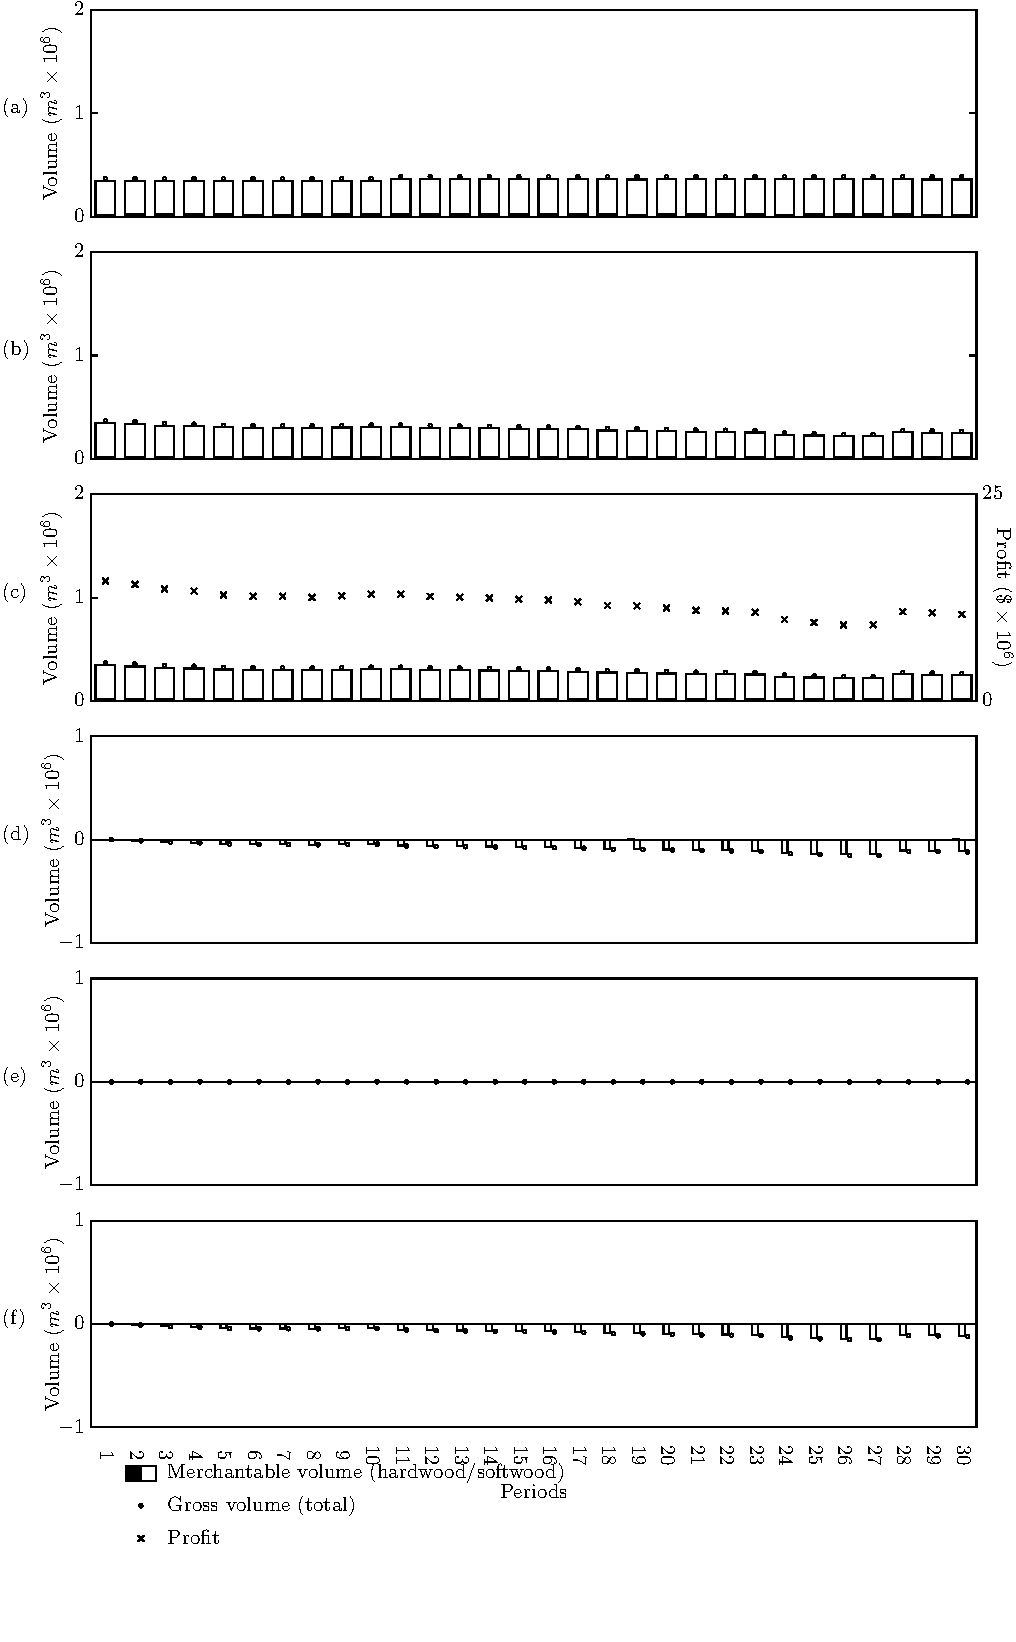
\includegraphics[width=10cm]{images/appendix/s6-1_p30a01}
  \caption{Reference sceanrio (i.e., base bilevel scenario)}
  \label{fig:s0_control}
\end{figure}

\begin{figure}[h]
  \centering
  \includegraphics[width=10cm]{images/appendix/s0_centralized}
  \caption{Scenario 0\_centralized (relax line-wise profitability constraint).}
  \label{fig:s0_centralized}
\end{figure}
   
%\chapter{Scenario Series 6-1}

This document presents simulation results from the scenario series 6-1, which tests impact of varying planning horizon length for both principal and agent. 
We test all combinations of horizon lengths for values 30, 20, 10, 5,  and 1 (periods). 
Note that agent horizon is never allowed to be longer than principal horizon.

\section{Summary}
Table \ref{tab:scenario_list} below lists the scenarios in series 6-1. 
Control scenario s6-0 simulates the \emph{status quo} situation (single-level wood supply model with no anticipation of fibre consumption).  

\begin{table}
  \centering
  \begin{tabular}{lll}
    \hline
    Scenario ID & Figure Reference & Description \\
    \hline
    6-0 & \ref{fig:s6-0} & Control scenario. \\
    6-1\_p30a30 & \ref{fig:s6-1_p30a30} & Principal: 30 periods, agent: 30 periods. \\
    6-1\_p30a20 & \ref{fig:s6-1_p30a20} & Principal: 30 periods, agent: 20 periods. \\
    6-1\_p30a10 & \ref{fig:s6-1_p30a10} & Principal: 30 periods, agent: 10 periods. \\
    6-1\_p30a05 & \ref{fig:s6-1_p30a05} & Principal: 30 periods, agent: 5 periods.   \\
    6-1\_p30a01 & \ref{fig:s6-1_p30a01} & Principal: 30 periods, agent: 1 period.     \\
    6-1\_p20a20 & \ref{fig:s6-1_p20a20} & Principal: 20 periods, agent: 20 periods.\\
    6-1\_p20a10 & \ref{fig:s6-1_p20a10} & Principal: 20 periods, agent: 10 periods.\\
    6-1\_p20a05 & \ref{fig:s6-1_p20a05} & Principal: 20 periods, agent: 5 periods. \\
    6-1\_p20a01 & \ref{fig:s6-1_p20a01} & Principal: 20 periods, agent: 1 period.  \\
    6-1\_p10a10 & \ref{fig:s6-1_p10a10} & Principal: 10 periods, agent: 10 periods.\\
    6-1\_p10a05 & \ref{fig:s6-1_p10a05} & Principal: 10 periods, agent: 5 periods. \\
    6-1\_p10a01 & \ref{fig:s6-1_p10a01} & Principal: 10 periods, agent: 1 period.  \\
    6-1\_p05a05 & \ref{fig:s6-1_p05a05} & Principal: 5 periods, agent: 5 periods. \\
    6-1\_p05a01 & \ref{fig:s6-1_p05a01} & Principal: 5 periods, agent: 1 period.  \\
    6-1\_p01a01 & \ref{fig:s6-1_p01a01} & Principal: 1 period, agent: 1 period.  \\
    \hline
  \end{tabular}
  \caption{Description of scenarios in series 6-4.}
  \label{tab:scenario_list}
\end{table}

\section{Results}

Figures \ref{fig:s6-1p30a30} to \ref{fig:s6-1p01a01} present
simulation results for fifteen scenarios. % Table \ref{tab:scenarios}
% summarizes scenario parameters used in the experiment for each
% scenario.
Disposition of figures is identical for all scenarios. The
first subfigure (a) for each scenario shows the initial
(ie. iteration-0) AAC solution. The second subfigure (b) for each
scenario shows first period of AAC solution for all 30 planning
iterations. The third subfigure (c) for each scenario shows the
implemented harvest level for all 30 planning iterations. Scenarios
3.1 and 3.2 also show profit in this subfigure on a secondary
axis. The fourth subfigure (d) for each scenario shows the difference
between initial and re-planned AAC. The fifth subfigure (e) for each
scenario shows the difference between re-planned AAC and harvest.  The
sixth subfigure (f) for each scenario shows the difference between
initial AAC and harvest. Softwood volume is shown with white bars,
hardwood volume with black bars, and total volume with small
circles. Profit (where applicable) is shown with the $\times$
symbol. 

\begin{figure}[h]
  \centering
  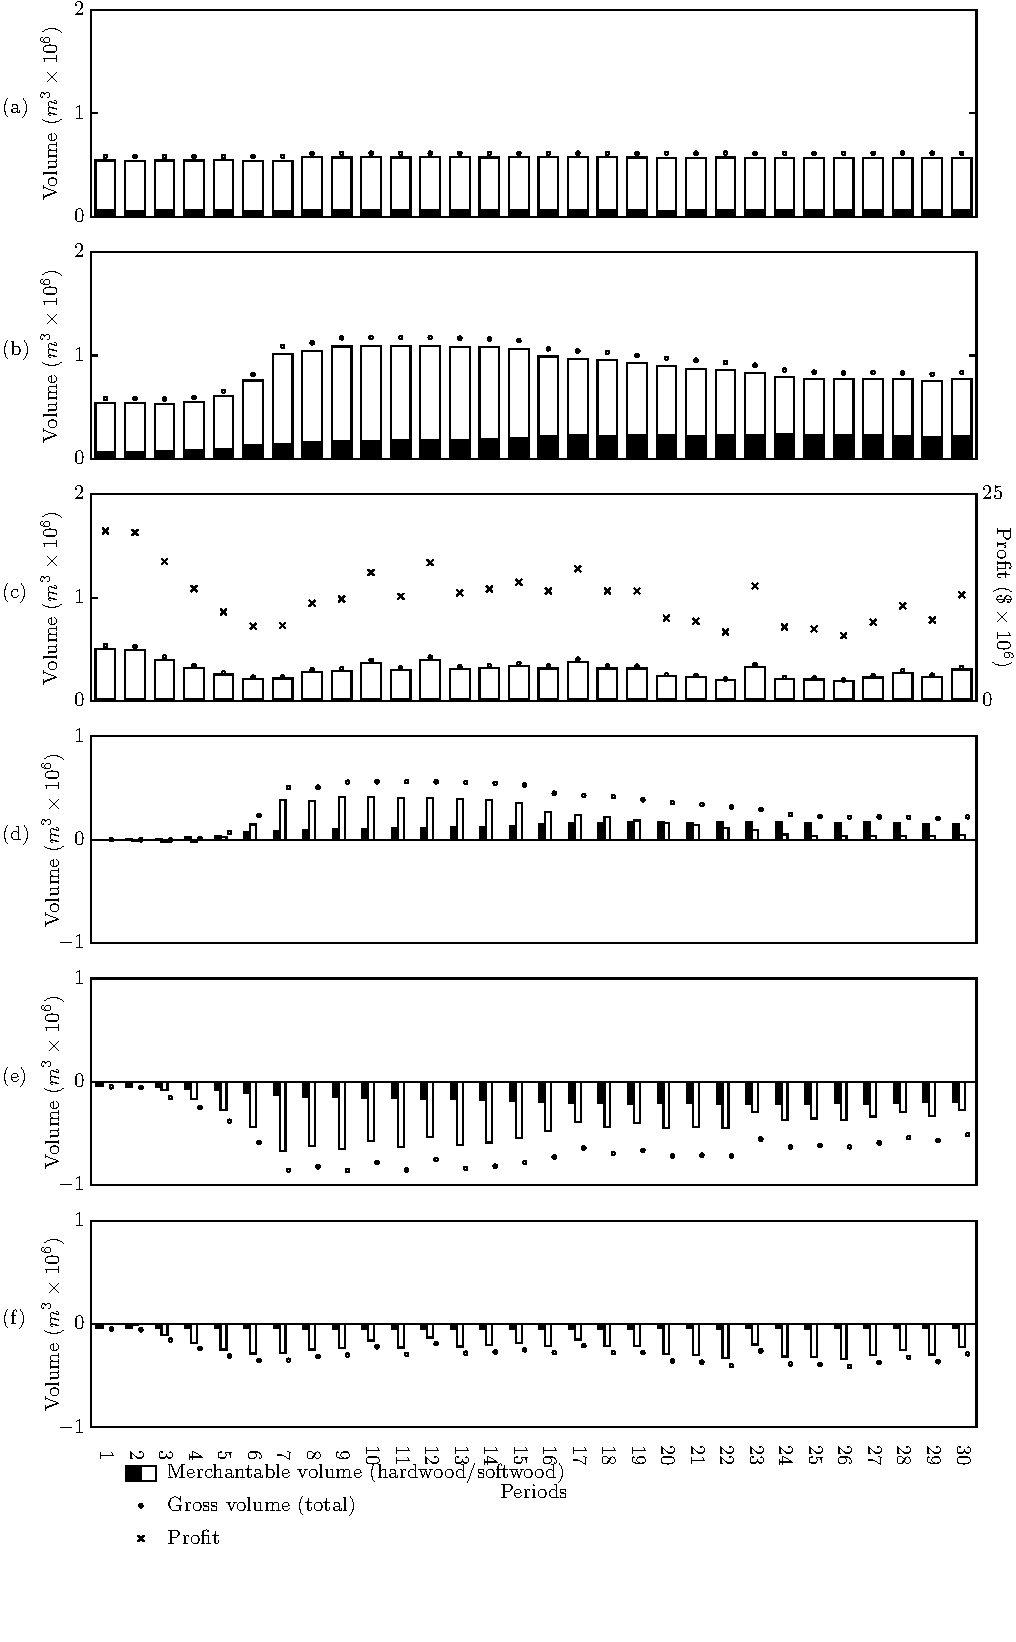
\includegraphics[width=10cm]{images/appendix/s6-0}
  \caption{Scenario 6-0 (control scenario, simulates \emph{status quo}).}
  \label{fig:s6-0}
\end{figure}


\begin{figure}[h]
  \centering
  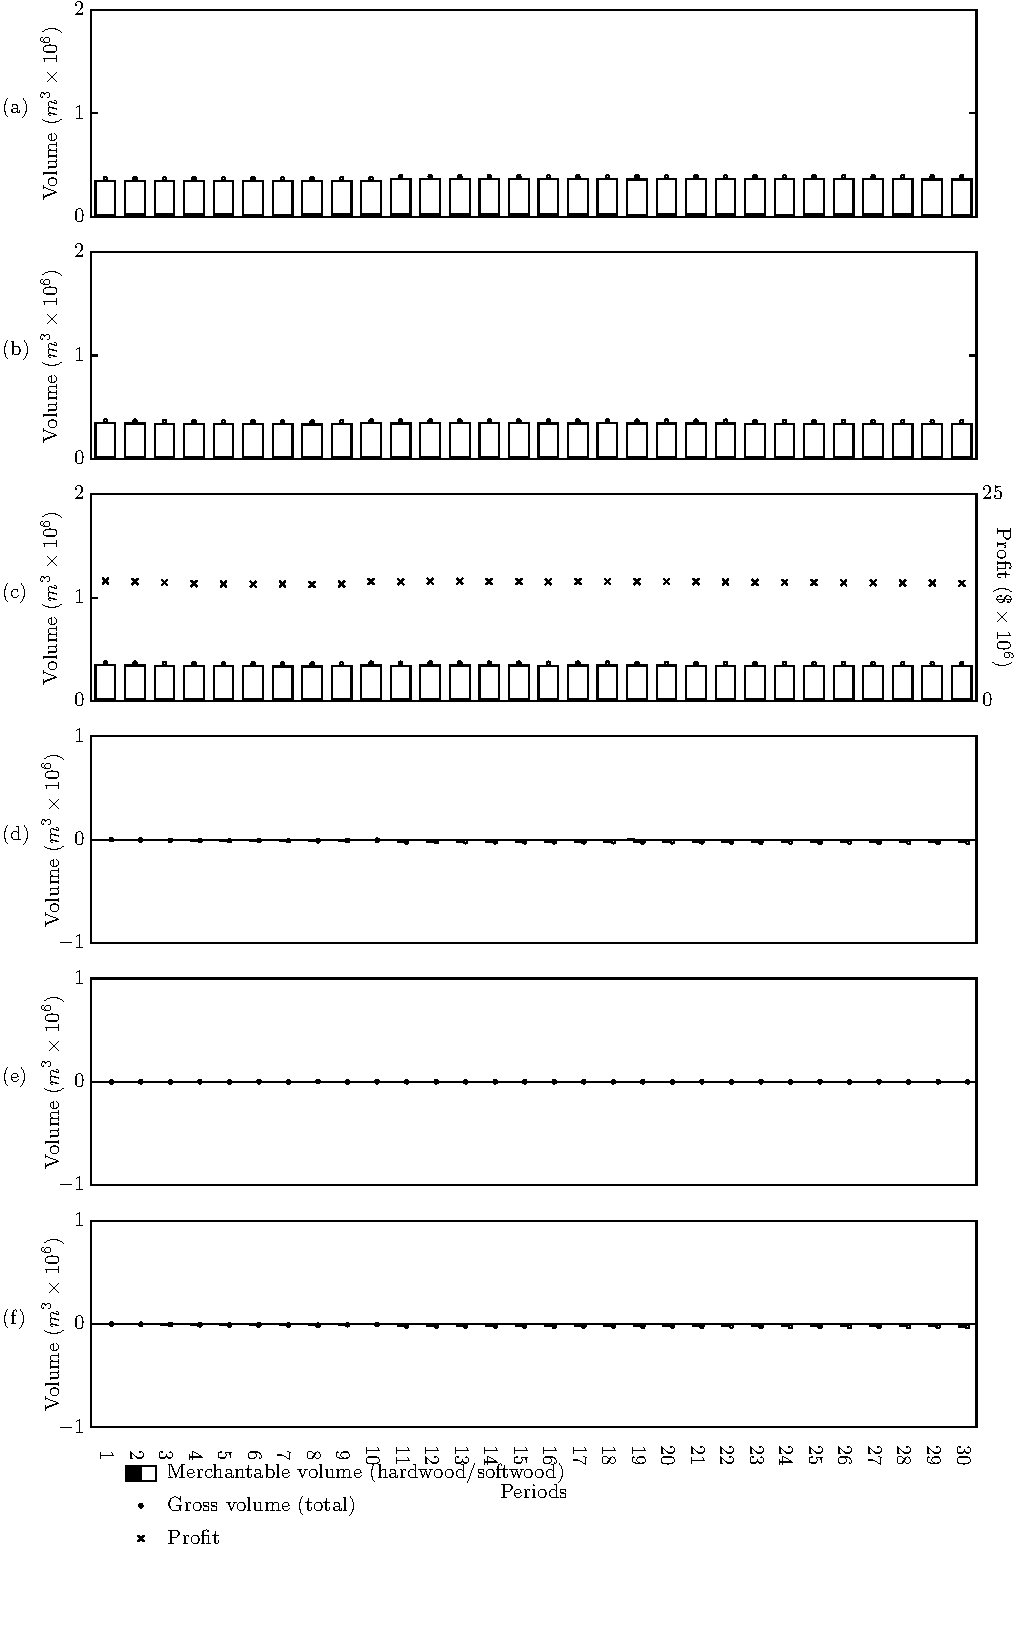
\includegraphics[width=10cm]{images/appendix/s6-1_p30a30}
  \caption{Scenario 6-1\_p30a30 (principal: 30 periods, agent: 30 periods).}
  \label{fig:s6-1_p30a30}
\end{figure}

\begin{figure}[h]
  \centering
  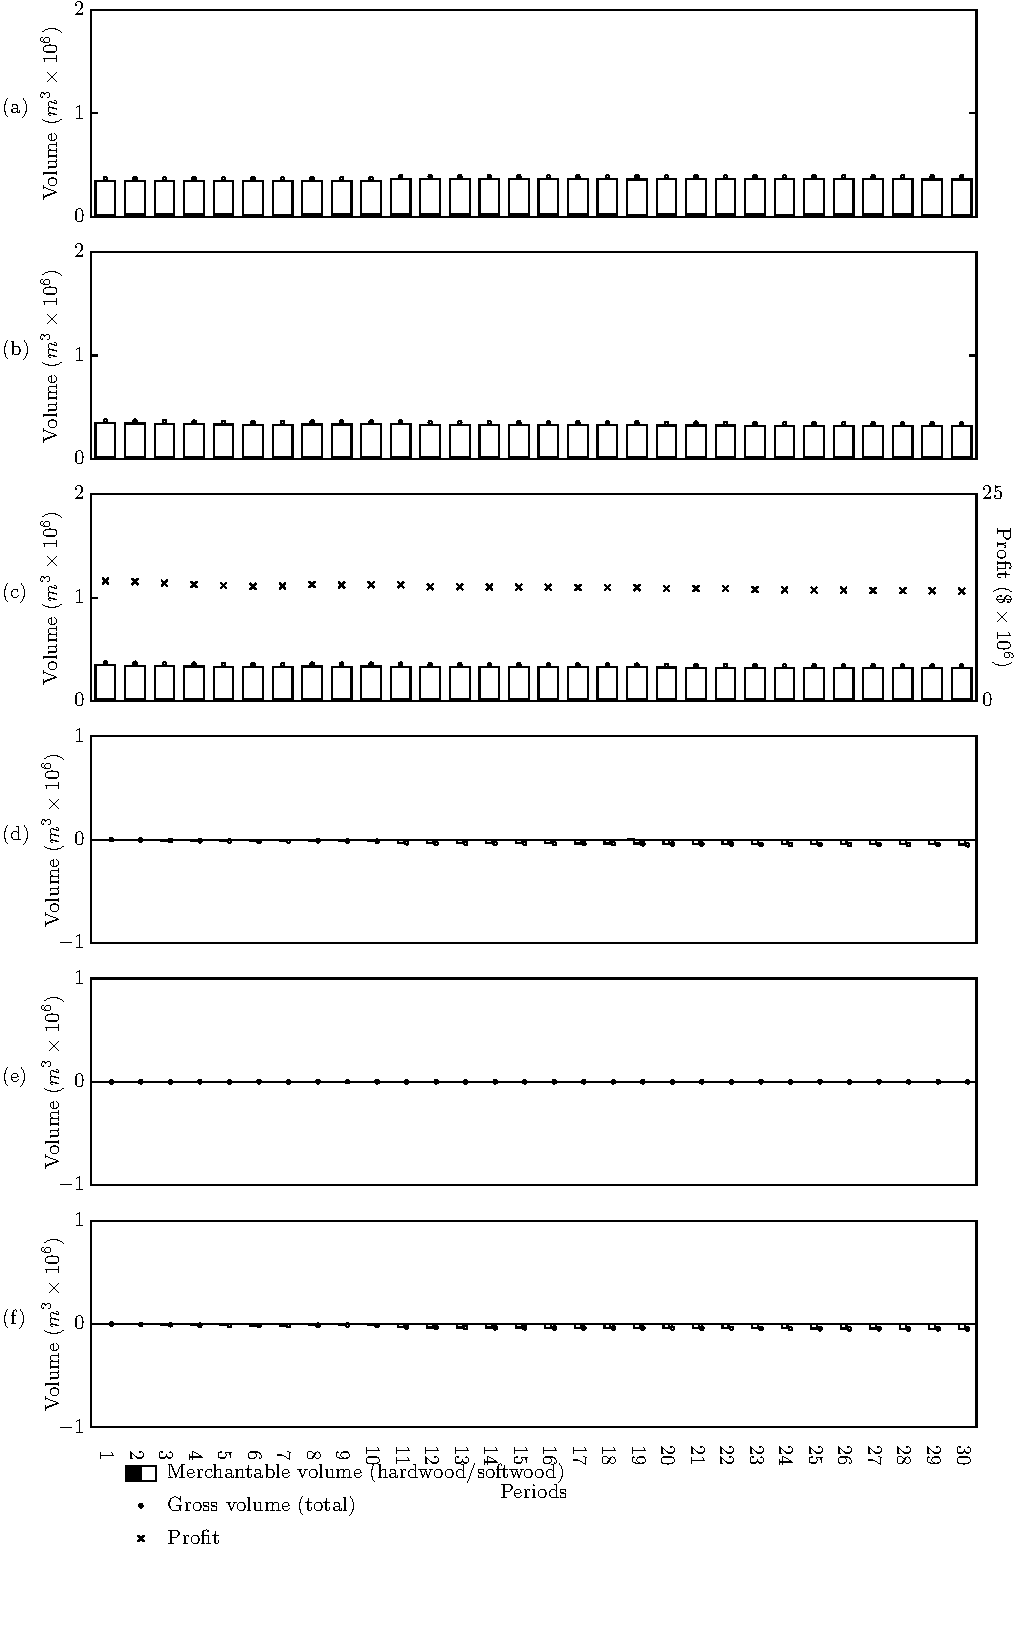
\includegraphics[width=10cm]{images/appendix/s6-1_p30a20}
  \caption{Scenario 6-1\_p30a20 (principal: 30 periods, agent: 20 periods).}
  \label{fig:s6-1_p30a20}
\end{figure}

\begin{figure}[h]
  \centering
  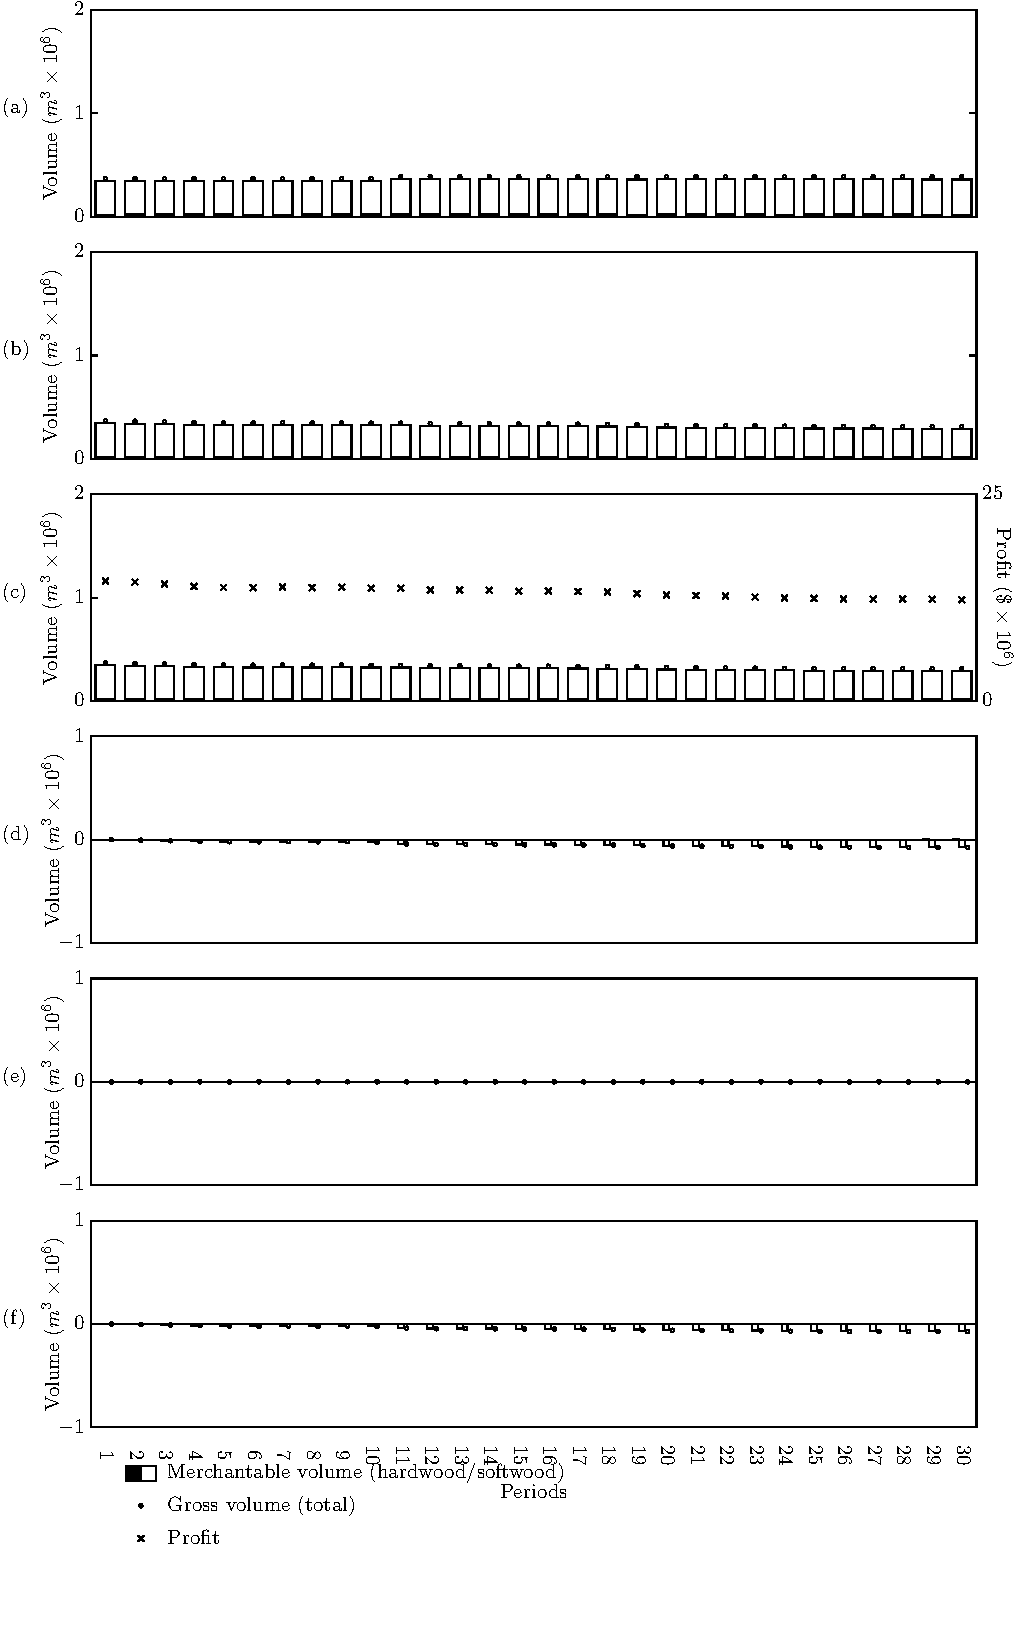
\includegraphics[width=10cm]{images/appendix/s6-1_p30a10}
  \caption{Scenario 6-1\_p30a10 (principal: 30 periods, agent: 10 periods).}
  \label{fig:s6-1_p30a10}
\end{figure}

\begin{figure}[h]
  \centering
  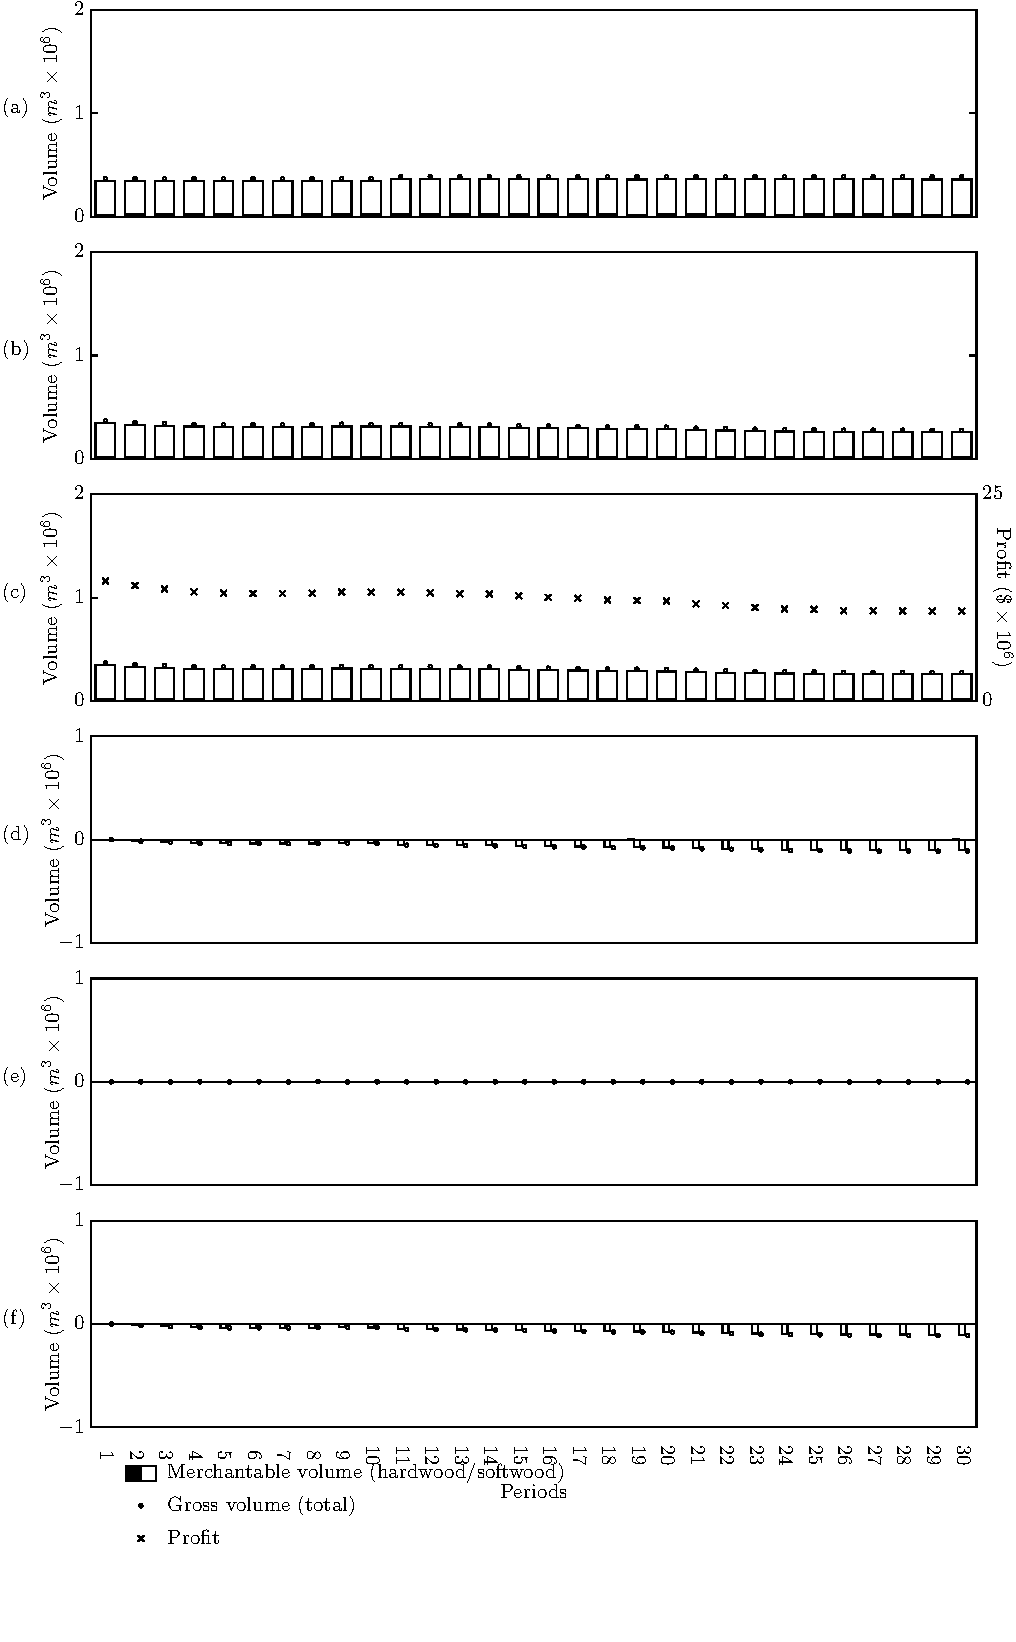
\includegraphics[width=10cm]{images/appendix/s6-1_p30a05}
  \caption{Scenario 6-1\_p30a05 (principal: 30 periods, agent: 5 periods).}
  \label{fig:s6-1_p30a05}
\end{figure}

\begin{figure}[h]
  \centering
  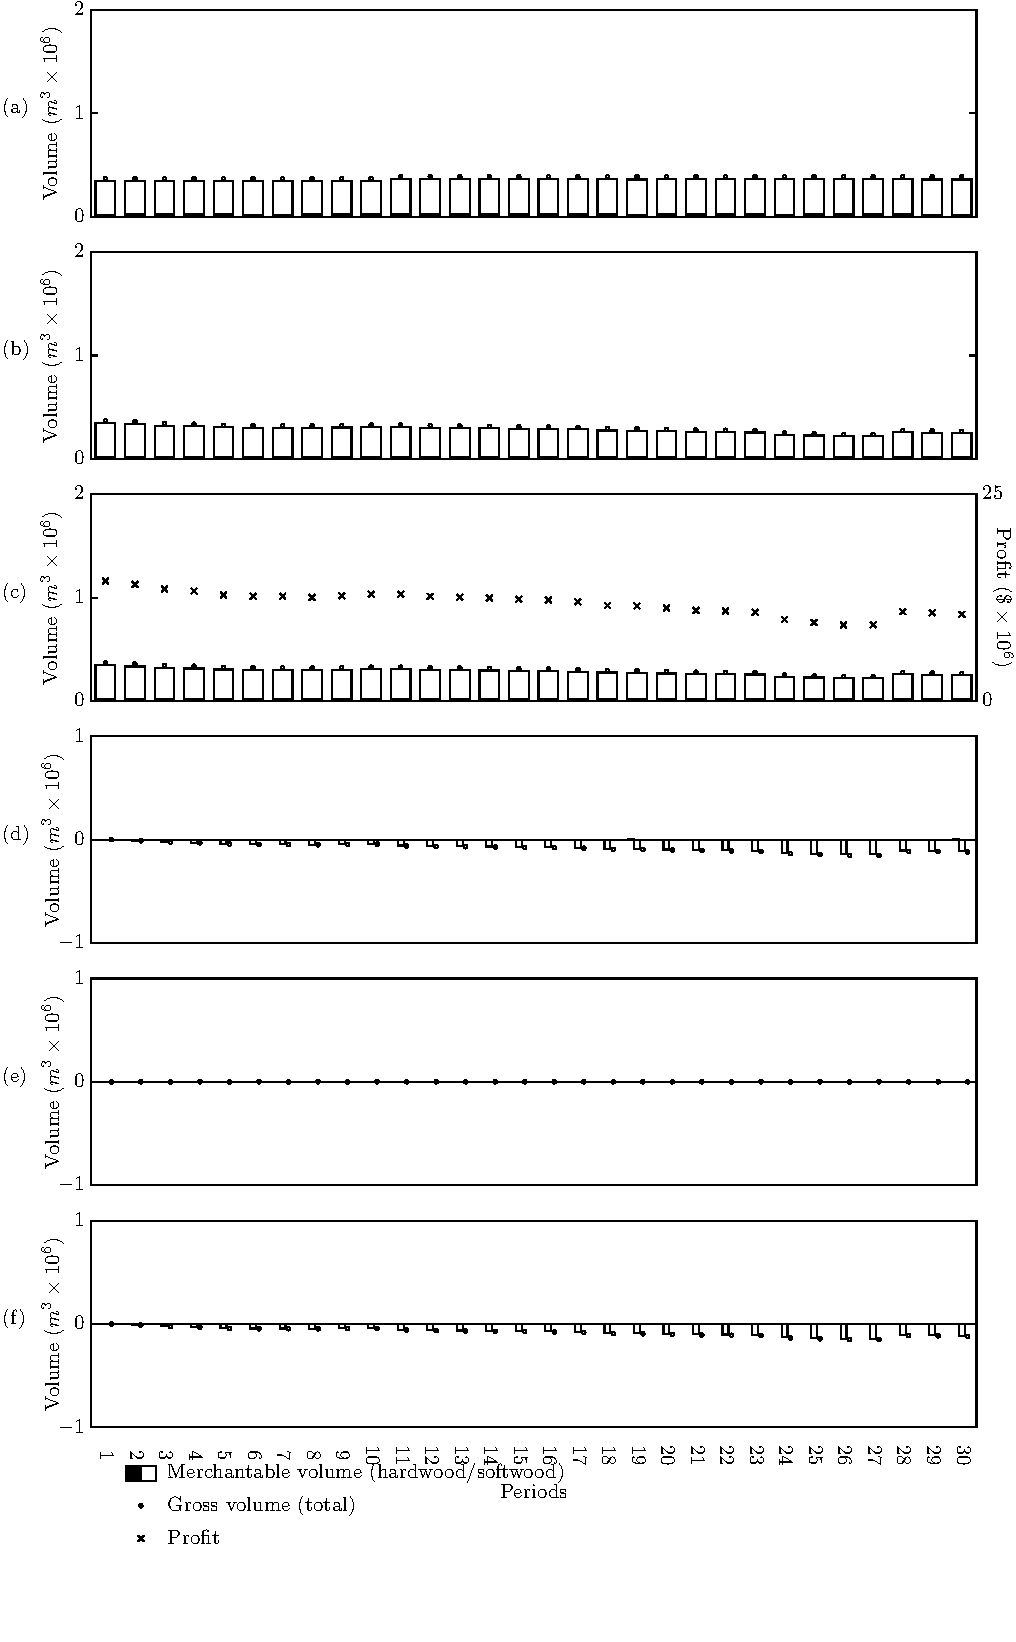
\includegraphics[width=10cm]{images/appendix/s6-1_p30a01}
  \caption{Scenario 6-1\_p30a01 (principal: 30 periods, agent: 1 period).}
  \label{fig:s6-1_p30a01}
\end{figure}


\begin{figure}[h]
  \centering
  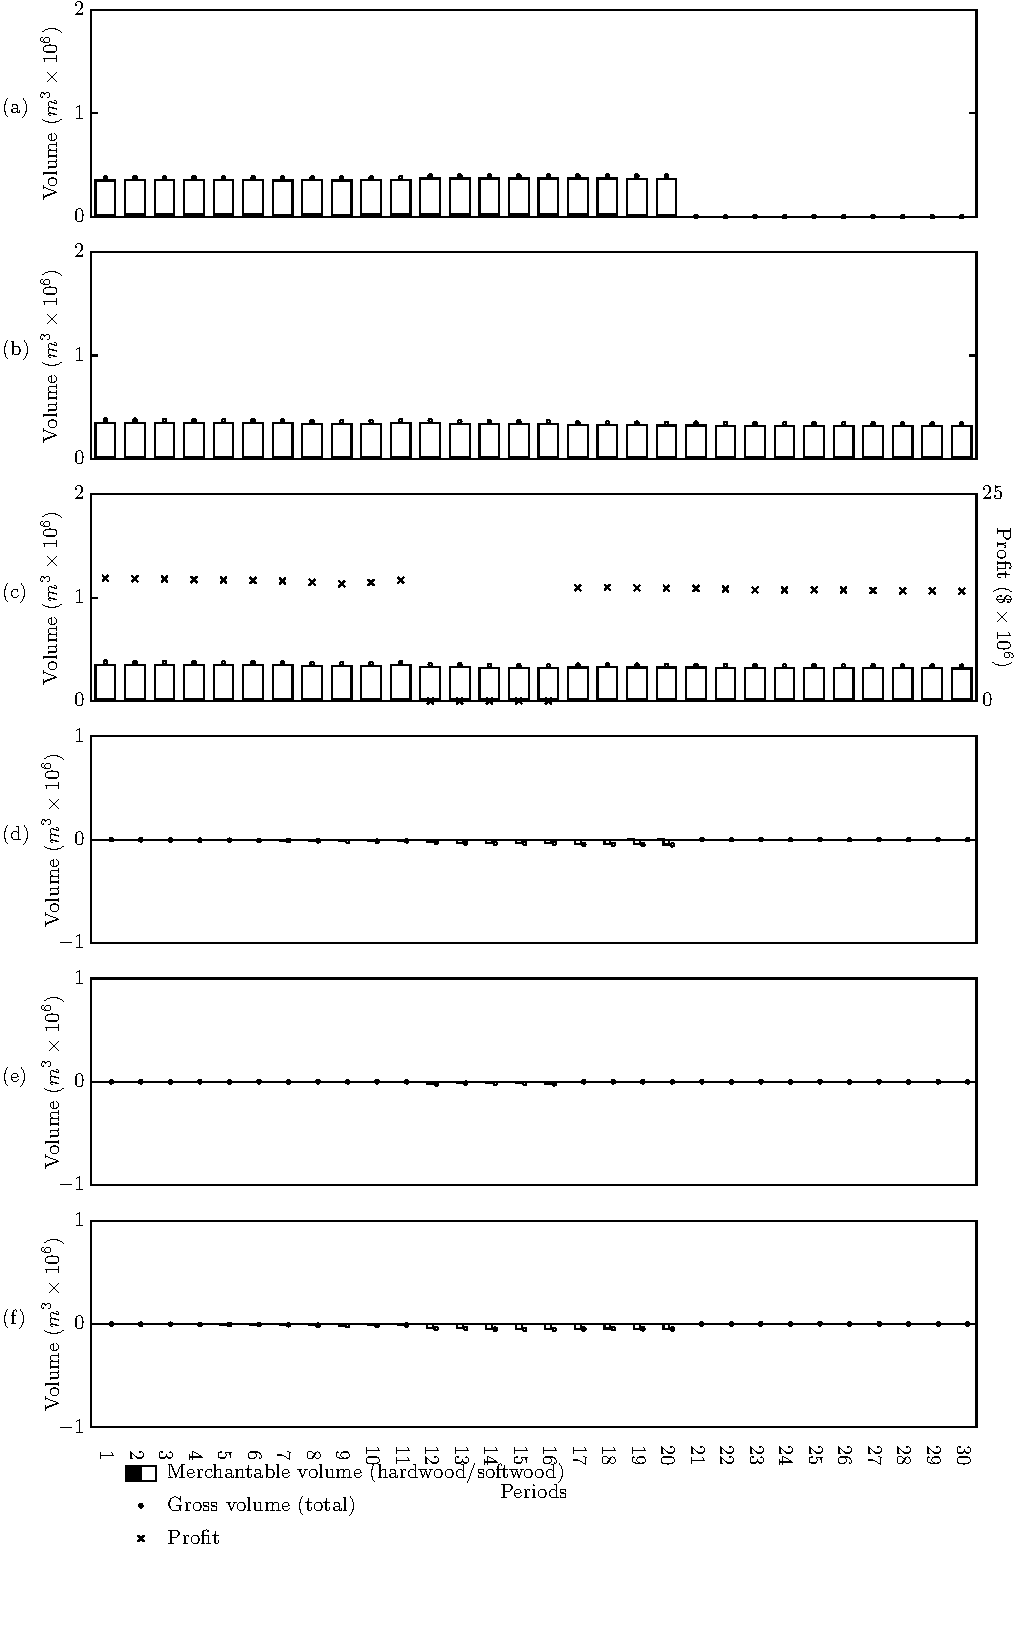
\includegraphics[width=10cm]{images/appendix/s6-1_p20a20}
  \caption{Scenario 6-1\_p20a20 (principal: 20 periods, agent: 20 periods).}
  \label{fig:s6-1_p20a20}
\end{figure}

\begin{figure}[h]
  \centering
  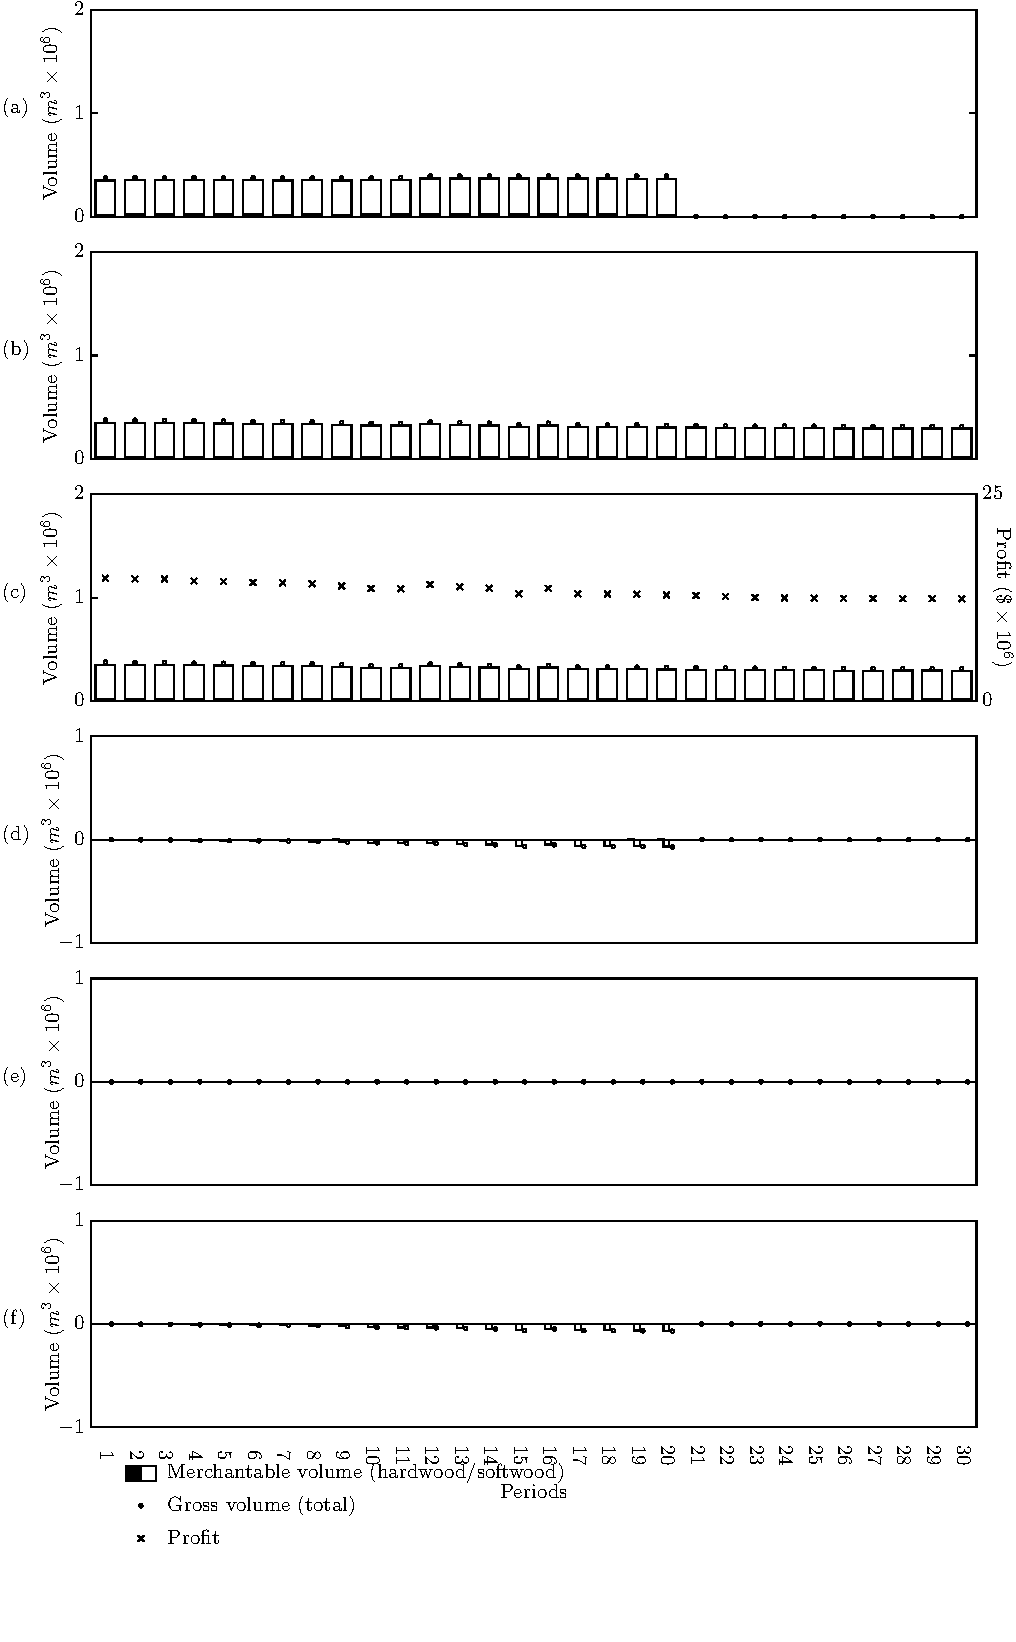
\includegraphics[width=10cm]{images/appendix/s6-1_p20a10}
  \caption{Scenario 6-1\_p20a10 (principal: 20 periods, agent: 10 periods).}
  \label{fig:s6-1_p20a10}
\end{figure}

\begin{figure}[h]
  \centering
  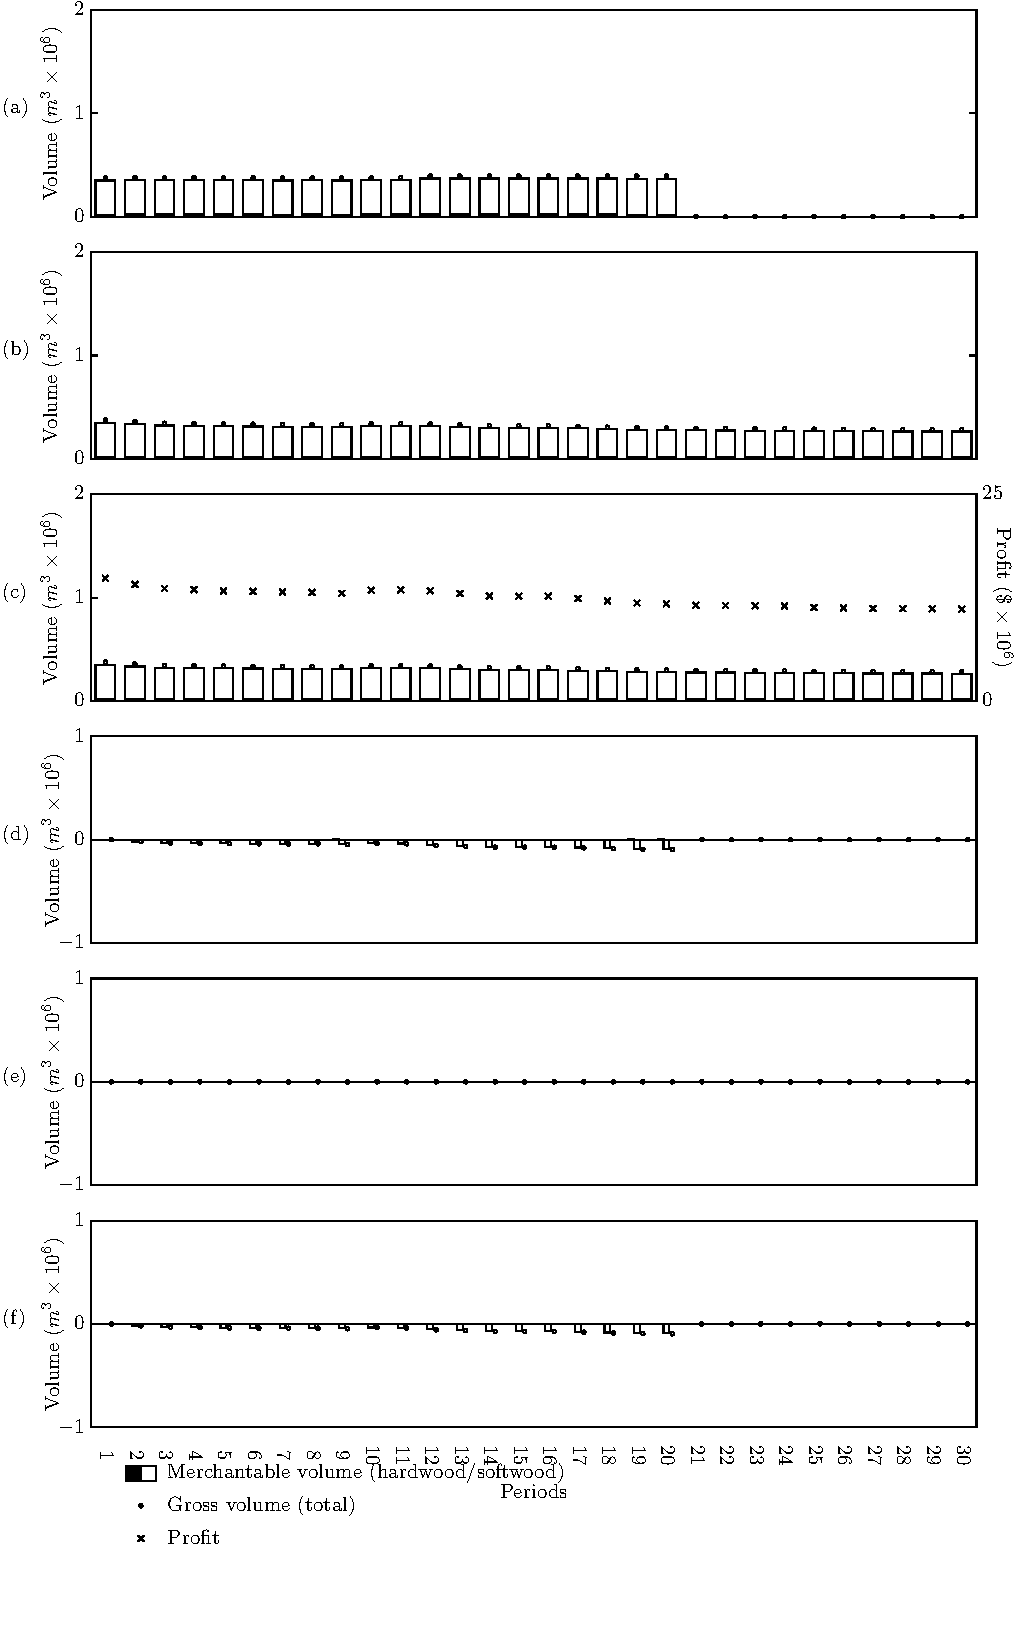
\includegraphics[width=10cm]{images/appendix/s6-1_p20a05}
  \caption{Scenario 6-1\_p20a05 (principal: 20 periods, agent: 5 periods).}
  \label{fig:s6-1_p20a05}
\end{figure}

\begin{figure}[h]
  \centering
  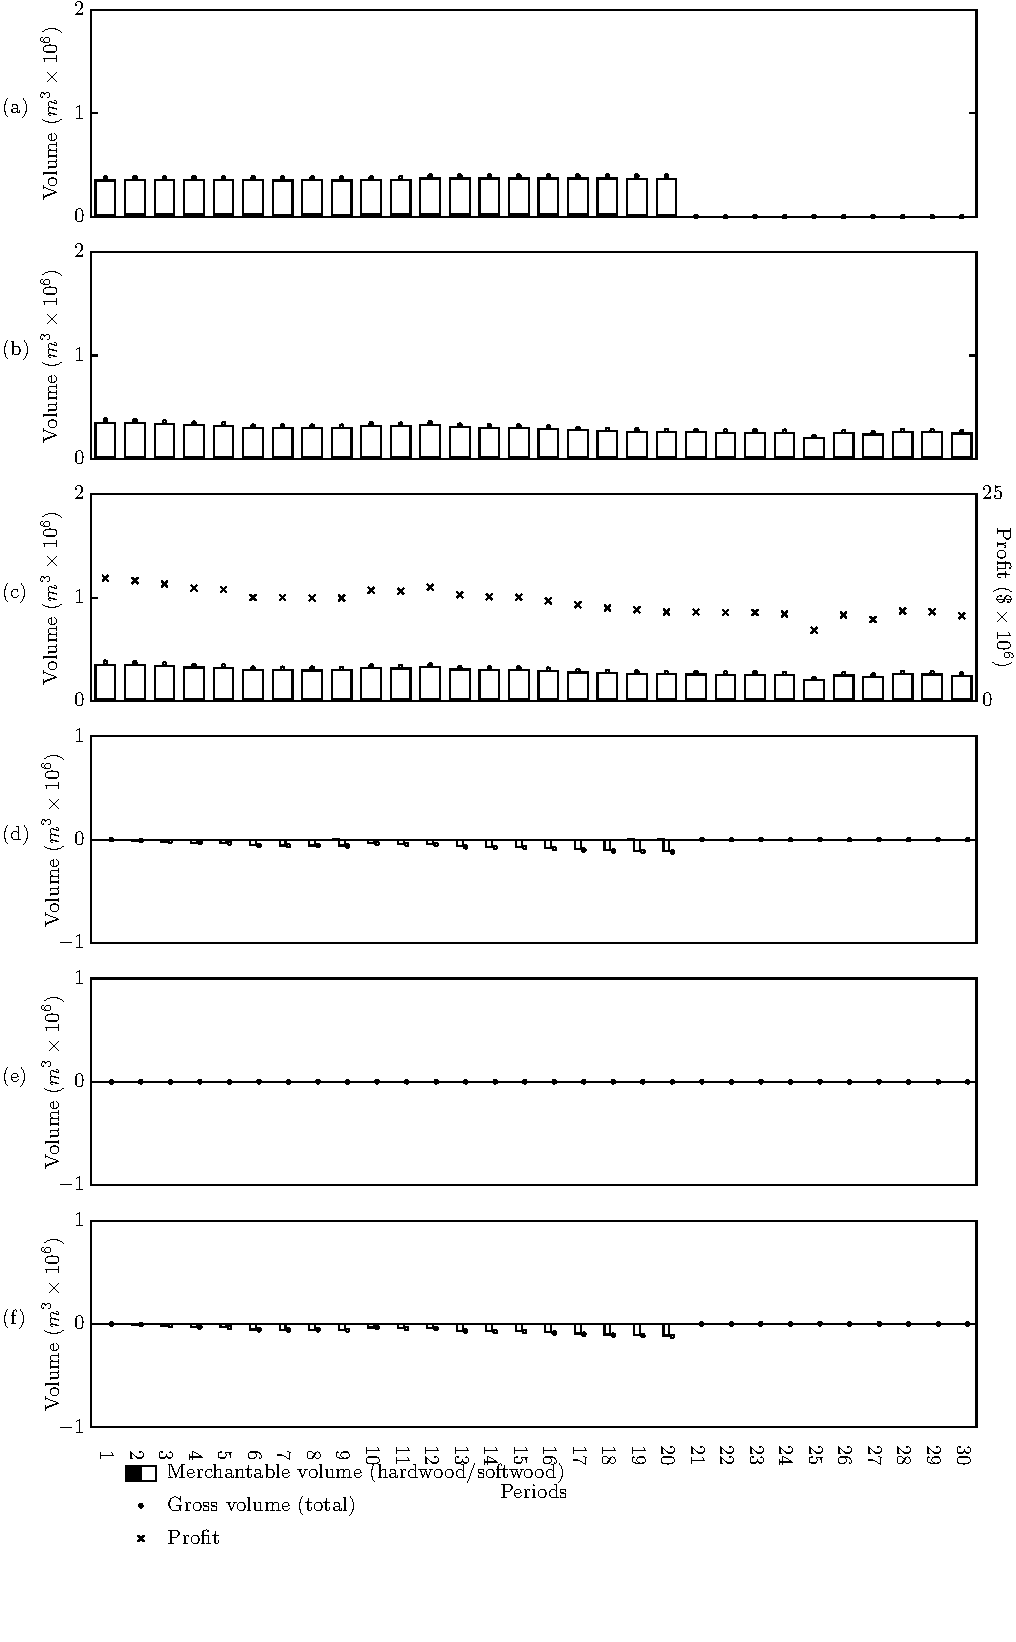
\includegraphics[width=10cm]{images/appendix/s6-1_p20a01}
  \caption{Scenario 6-1\_p20a01 (principal: 20 periods, agent: 1 period).}
  \label{fig:s6-1_p20a01}
\end{figure}


\begin{figure}[h]
  \centering
  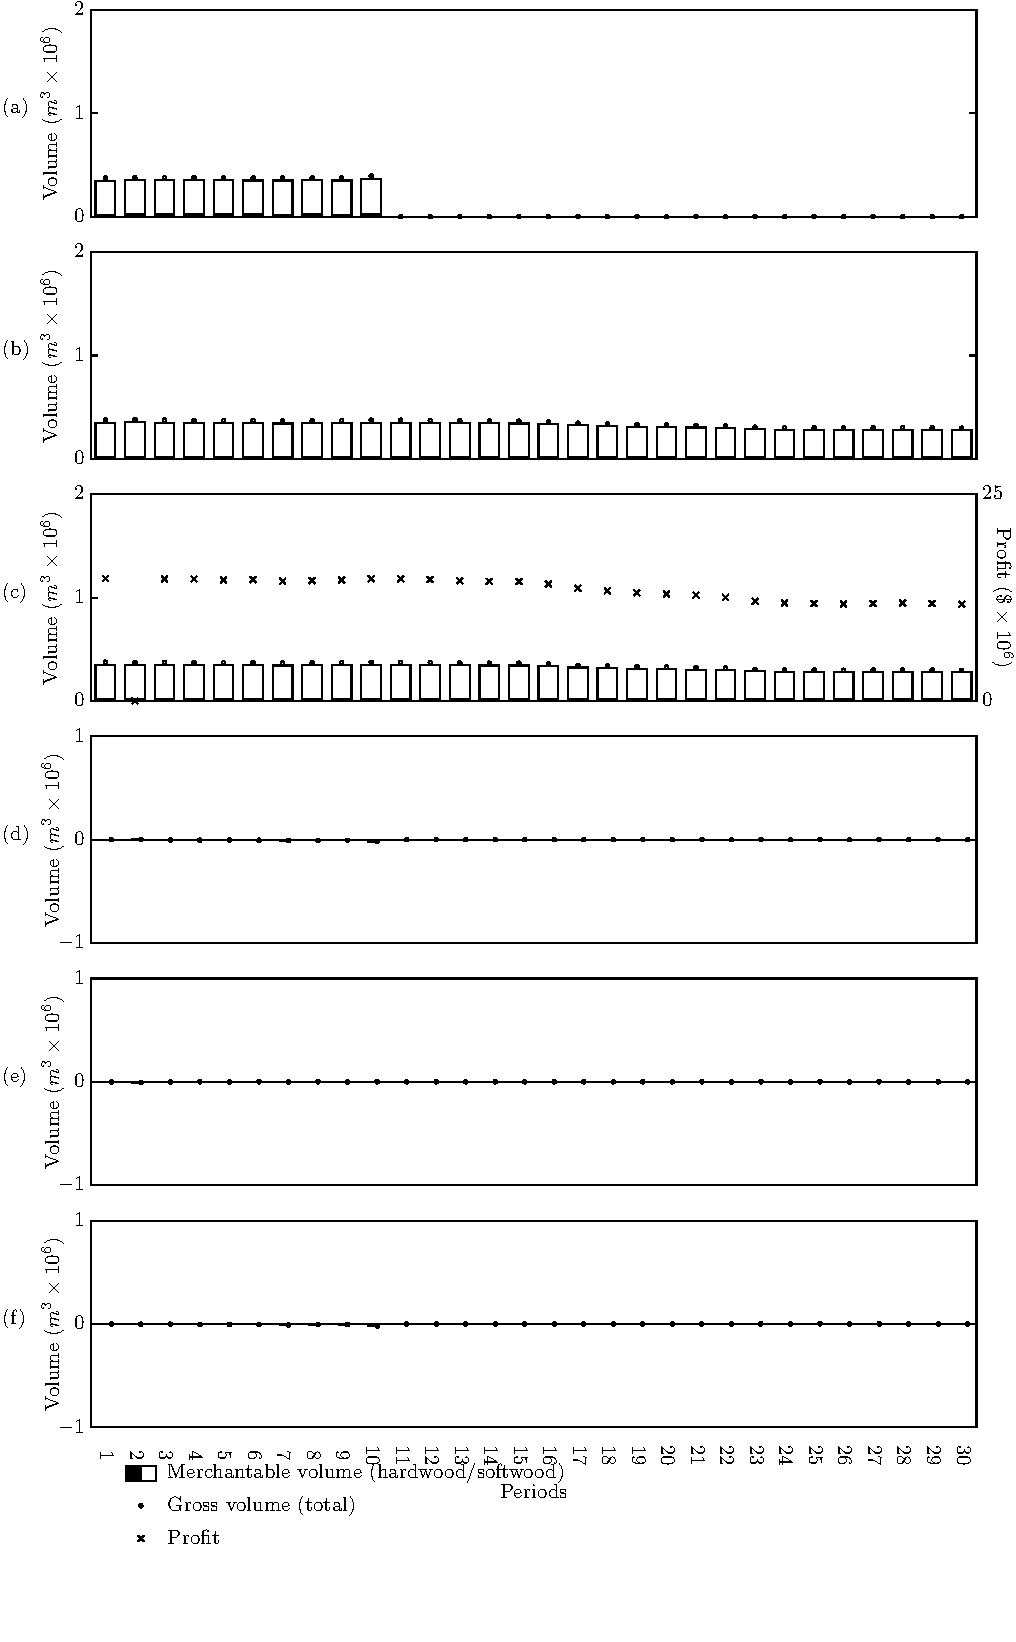
\includegraphics[width=10cm]{images/appendix/s6-1_p10a10}
  \caption{Scenario 6-1\_p10a10 (principal: 10 periods, agent: 10 periods).}
  \label{fig:s6-1_p10a10}
\end{figure}

\begin{figure}[h]
  \centering
  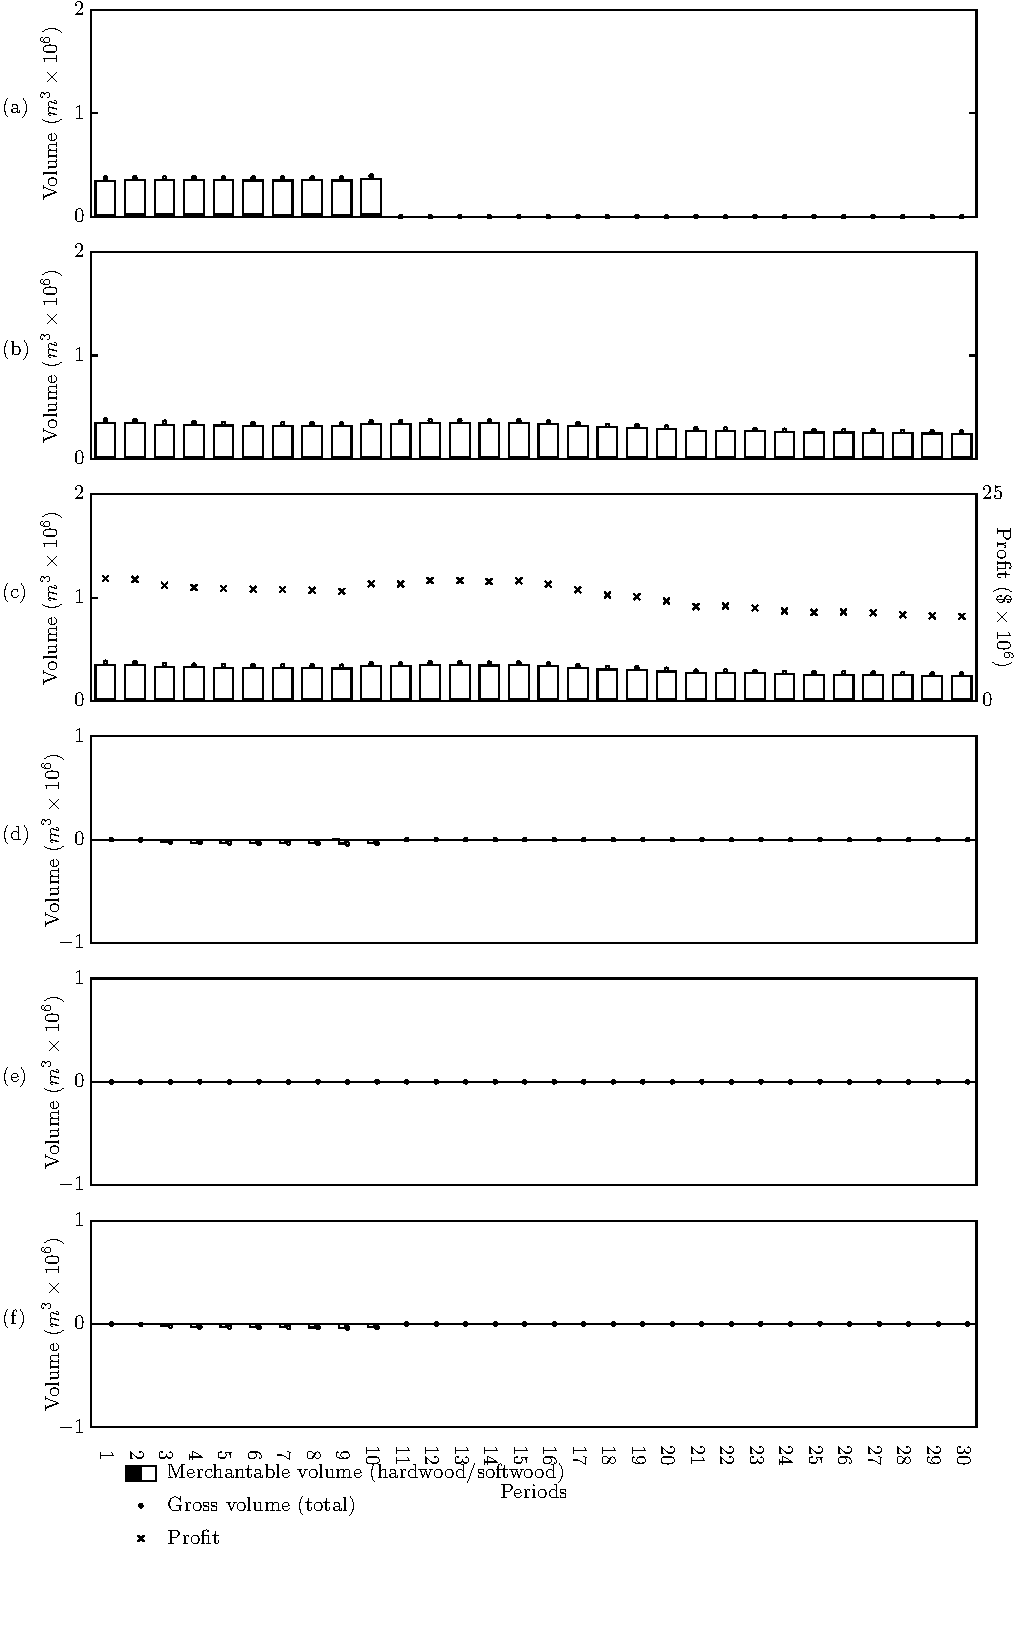
\includegraphics[width=10cm]{images/appendix/s6-1_p10a05}
  \caption{Scenario 6-1\_p10a05 (principal: 10 periods, agent: 5 periods).}
  \label{fig:s6-1_p10a05}
\end{figure}

\begin{figure}[h]
  \centering
  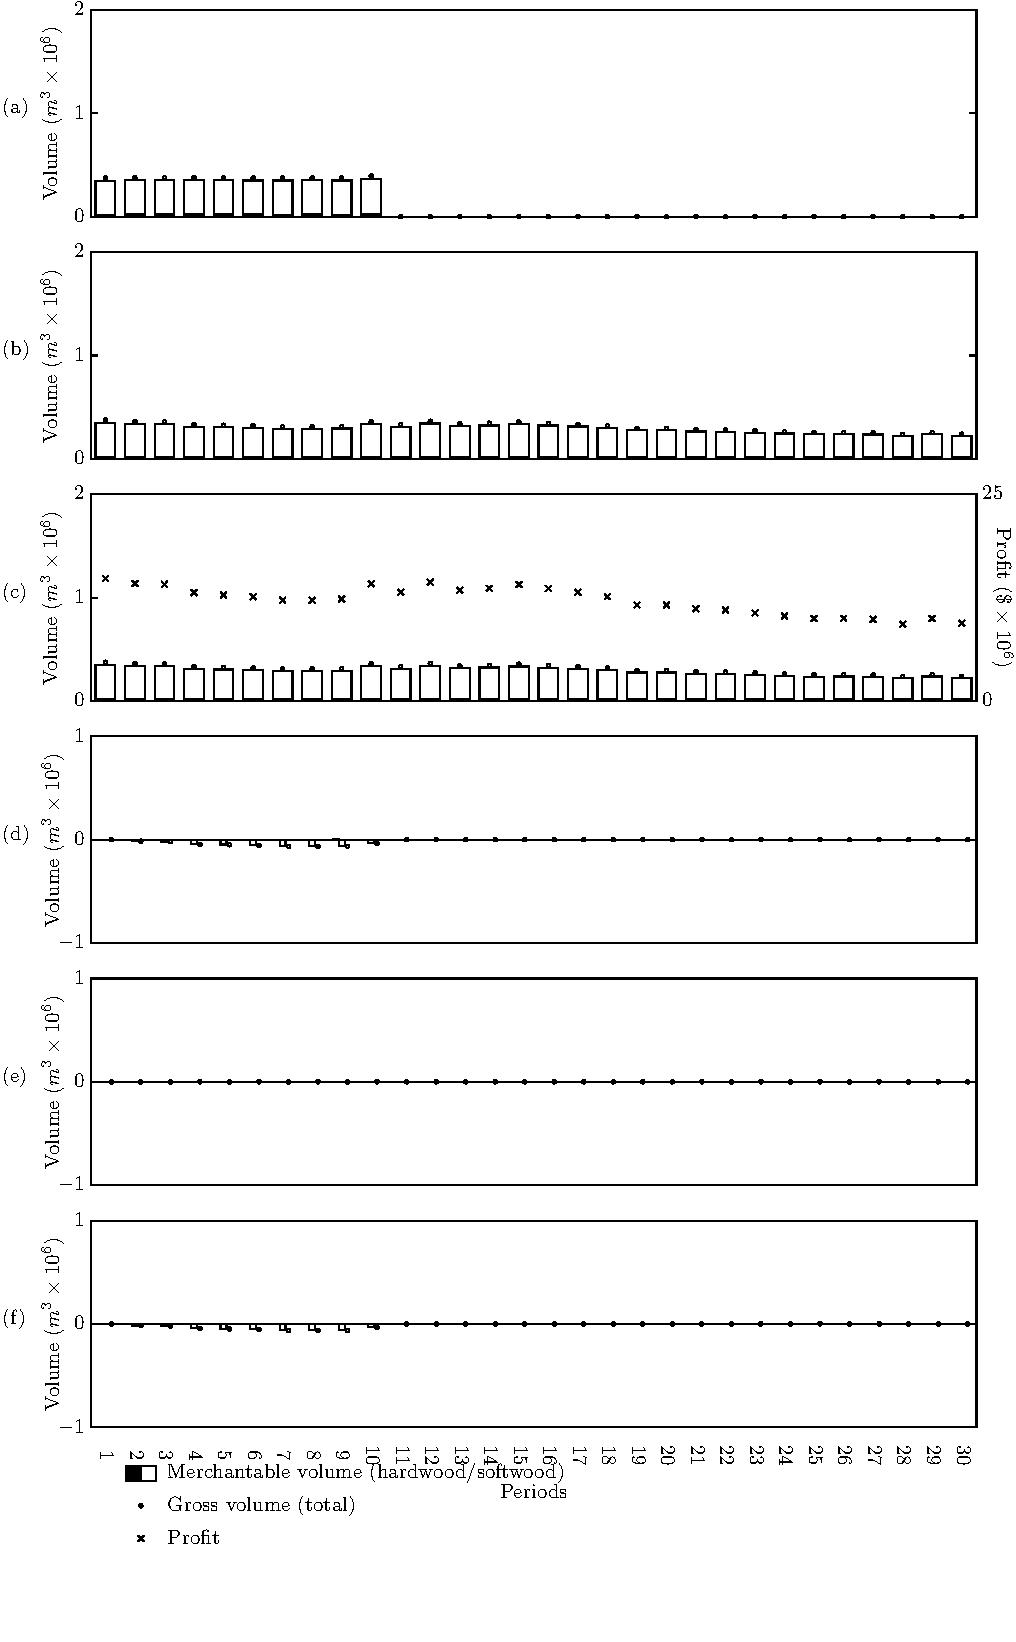
\includegraphics[width=10cm]{images/appendix/s6-1_p10a01}
  \caption{Scenario 6-1\_p10a01 (principal: 10 periods, agent: 1 period).}
  \label{fig:s6-1_p10a01}
\end{figure}


\begin{figure}[h]
  \centering
  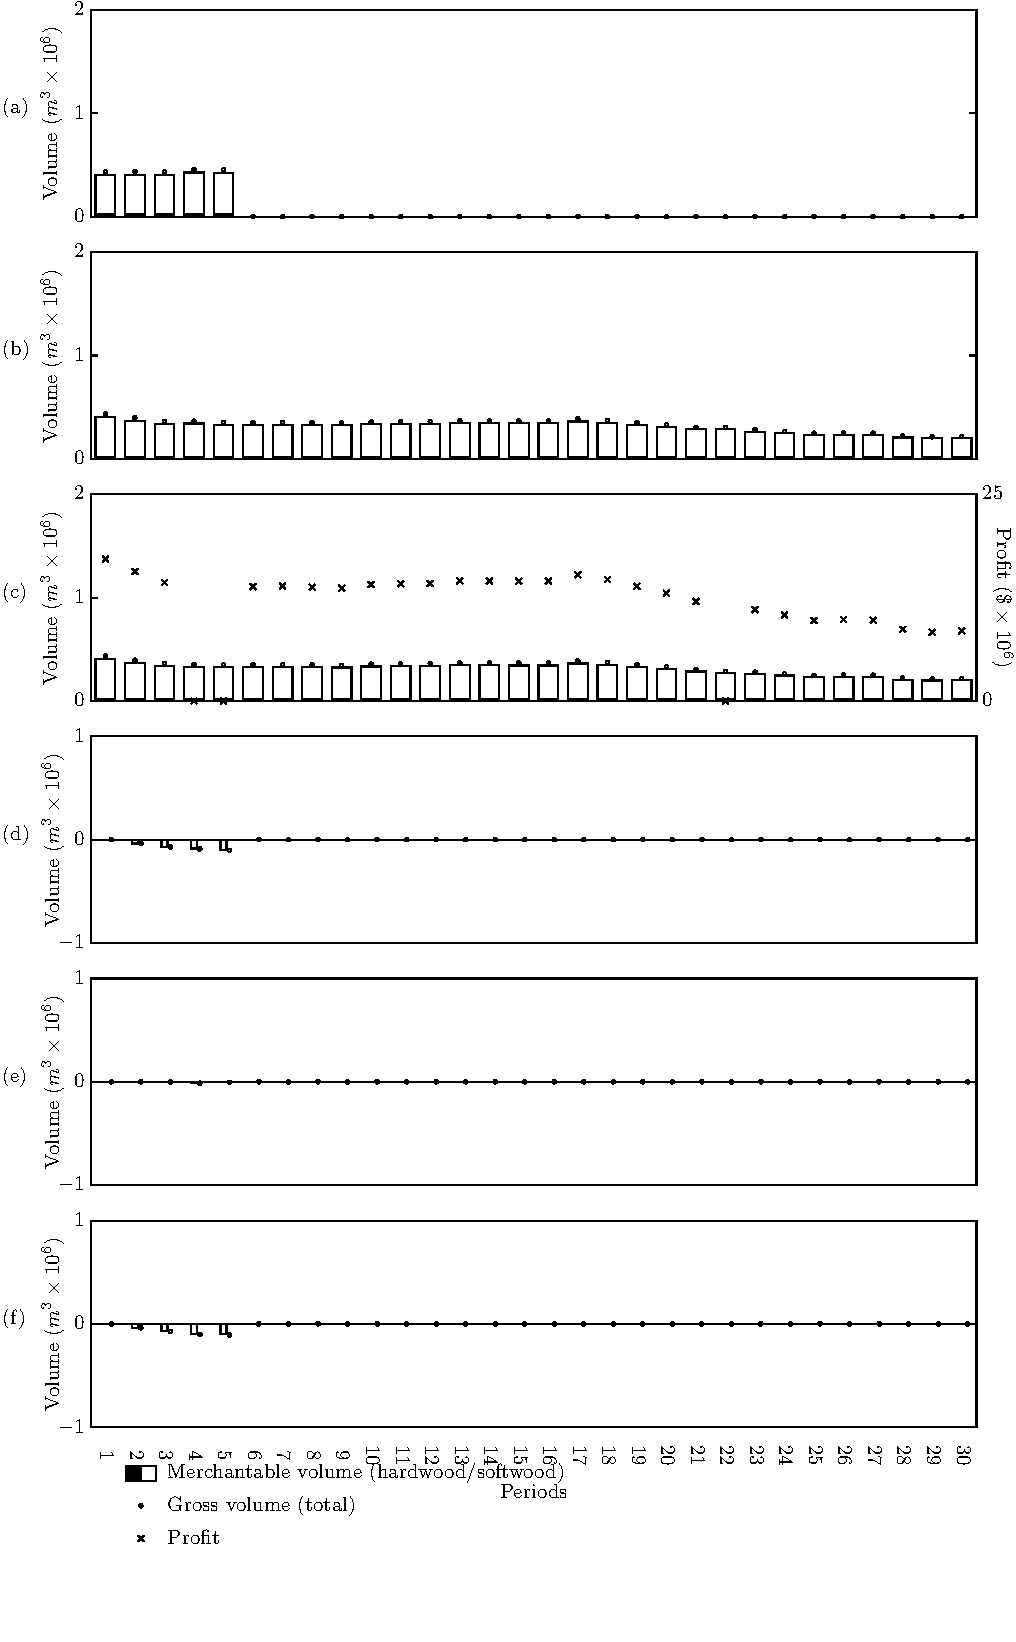
\includegraphics[width=10cm]{images/appendix/s6-1_p05a05}
  \caption{Scenario 6-1\_p05a05 (principal: 05 periods, agent: 5 periods).}
  \label{fig:s6-1_p05a05}
\end{figure}

\begin{figure}[h]
  \centering
  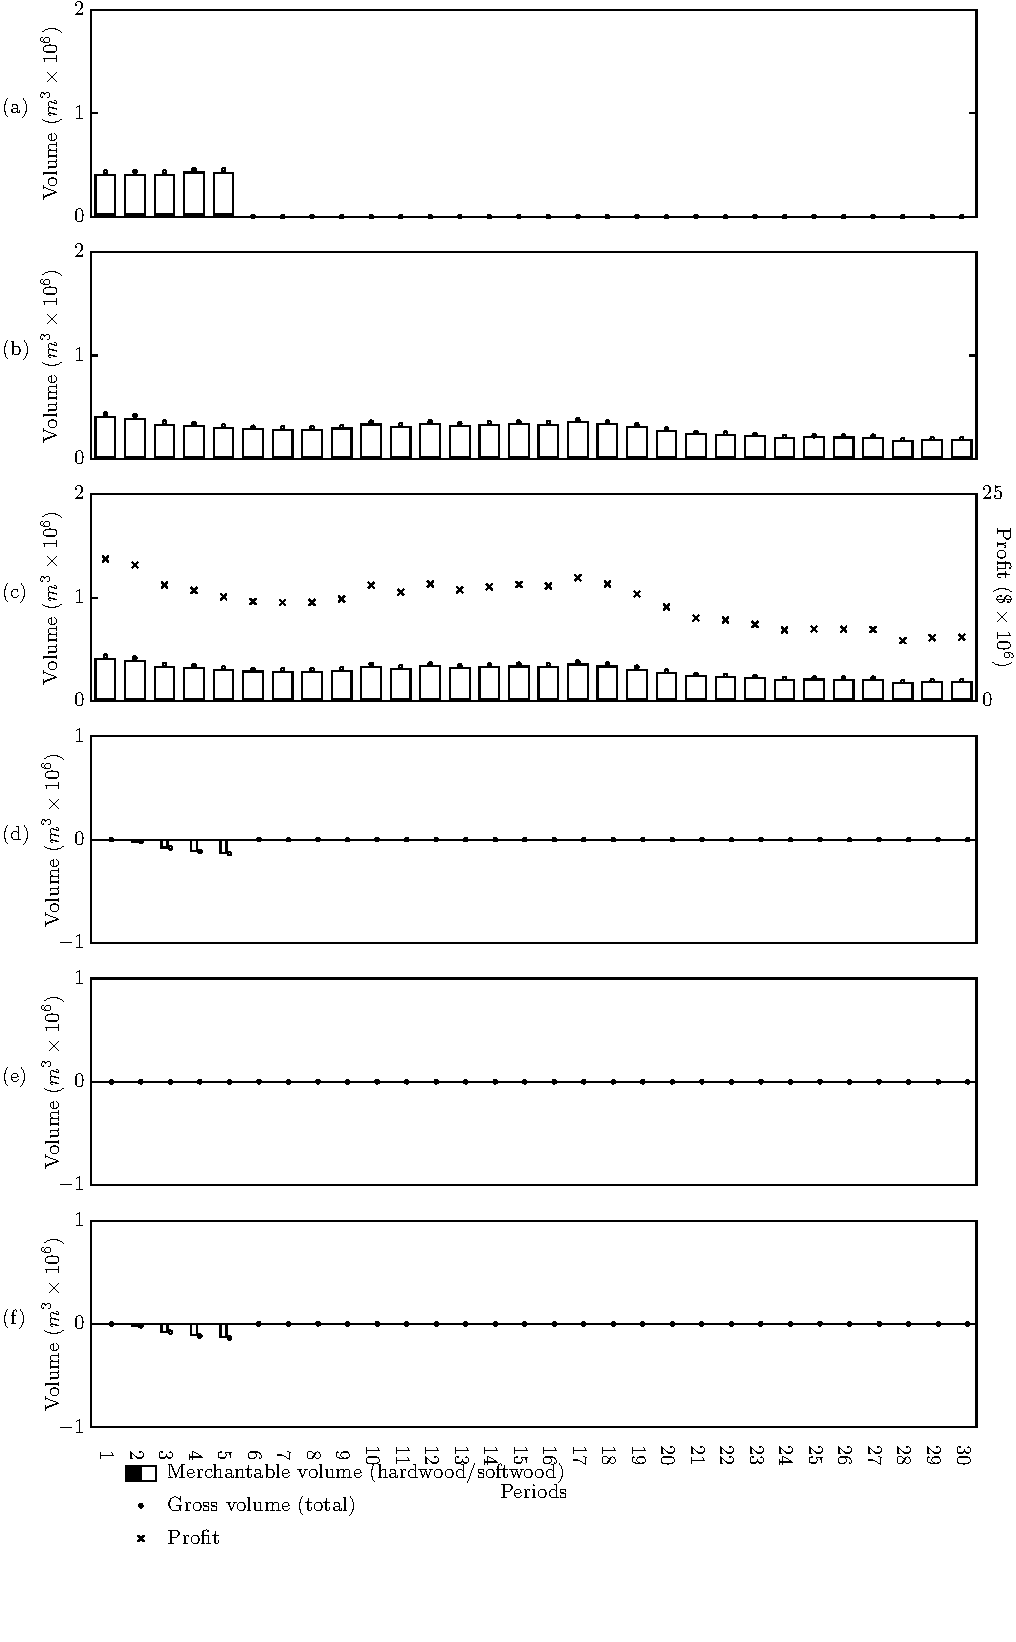
\includegraphics[width=10cm]{images/appendix/s6-1_p05a01}
  \caption{Scenario 6-1\_p05a01 (principal: 05 periods, agent: 1 period).}
  \label{fig:s6-1_p05a01}
\end{figure}


\begin{figure}[h]
  \centering
  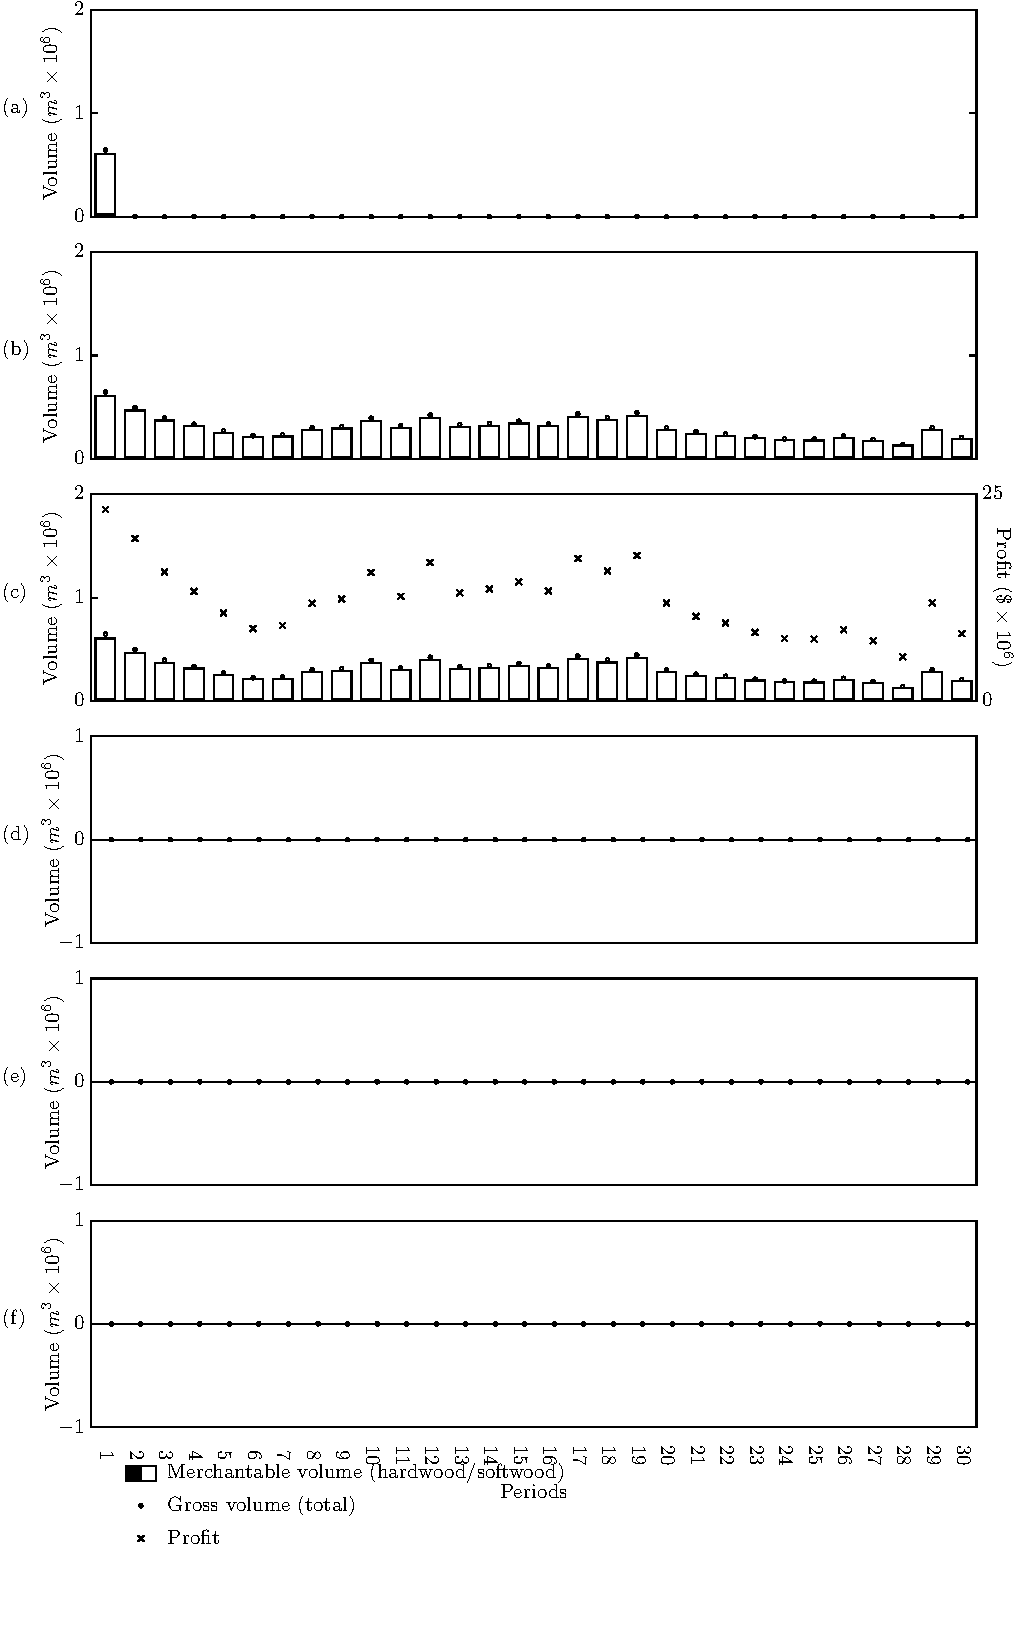
\includegraphics[width=10cm]{images/appendix/s6-1_p01a01}
  \caption{Scenario 6-1\_p01a01 (principal: 1 period, agent: 1 period).}
  \label{fig:s6-1_p01a01}
\end{figure}
   
%\chapter{Scenario Series 6-2x}

This appendix presents simulation results from the 6-2x scenario series, which tests the impact of increasing end-product prices in the agent network. We increase all products prices proportionately (i.e., perfectly correlated price increase, relative to base values), and keep them constant for all 30 iterations. 

\section{Summary}
Table \ref{tab:scenario_list} below lists the scenarios in series 6-2x.
 
Base scenario s6-2x\_f1.0 is identical to s6-1\_p30a01, and simulates a basic bilevel scenario with default prices (i.e., scaling factor 1.0).
Scaling factors used for other scenarios are listed in Table \ref{tab:scenario_list}. The values for the scaling factors may seem a bit odd (vary between $1.6$ and $7.1$), but these are the due to some unexpected side-effects in the code I hijacked to generate these scenarios. These were initially intended as debugging runs, but ended up revealing some interesting aspects of the model worthwhile reporting.

Somewhere between f4.0 and f4.6, there is a sudden change in model behaviour.

\begin{table}
  \centering
  \begin{tabular}{lll}
    \hline
    Scenario ID & Figure Reference & Description \\
    \hline
    6-2x\_f1.0 & \ref{fig:s6-2x_test00} & Control scenario (same as s6-1\_p30a01). \\
    6-2x\_f1.6 & \ref{fig:s6-2x_test10} & Prices scaled by factor of 1.6 \\
    6-2x\_f2.2 & \ref{fig:s6-2x_test20} & Prices scaled by factor of 2.2 \\
    6-2x\_f2.8 & \ref{fig:s6-2x_test30} & Prices scaled by factor of 2.8 \\
    6-2x\_f3.4 & \ref{fig:s6-2x_test40} & Prices scaled by factor of 3.4 \\
    6-2x\_f4.0 & \ref{fig:s6-2x_test50} & Prices scaled by factor of 4.0 \\
    6-2x\_f4.6 & \ref{fig:s6-2x_test60} & Prices scaled by factor of 4.6 \\
    6-2x\_f5.3 & \ref{fig:s6-2x_test70} & Prices scaled by factor of 5.3 \\
    6-2x\_f5.9 & \ref{fig:s6-2x_test80} & Prices scaled by factor of 5.9 \\
    6-2x\_f6.4 & \ref{fig:s6-2x_test90} & Prices scaled by factor of 6.4 \\
    6-2x\_f7.1 & \ref{fig:s6-2x_test100} & Prices scaled by factor of 7.1 \\
    \hline
  \end{tabular}
  \caption{Description of scenarios in series 6-2x.}
  \label{tab:scenario_list}
\end{table}


\section{Results}

Figures \ref{fig:s6-2x_test00} to \ref{fig:s6-2x_test100} present
simulation results for fifteen scenarios. % Table \ref{tab:scenarios}
% summarizes scenario parameters used in the experiment for each
% scenario.
Disposition of figures is identical for all scenarios. The
first subfigure (a) for each scenario shows the initial
(ie. iteration-0) AAC solution. The second subfigure (b) for each
scenario shows first period of AAC solution for all 30 planning
iterations. The third subfigure (c) for each scenario shows the
implemented harvest level for all 30 planning iterations. Scenarios
3.1 and 3.2 also show profit in this subfigure on a secondary
axis. The fourth subfigure (d) for each scenario shows the difference
between initial and re-planned AAC. The fifth subfigure (e) for each
scenario shows the difference between re-planned AAC and harvest.  The
sixth subfigure (f) for each scenario shows the difference between
initial AAC and harvest. Softwood volume is shown with white bars,
hardwood volume with black bars, and total volume with small
circles. Profit (where applicable) is shown with the $\times$
symbol. 


\begin{figure}[h]
  \centering
  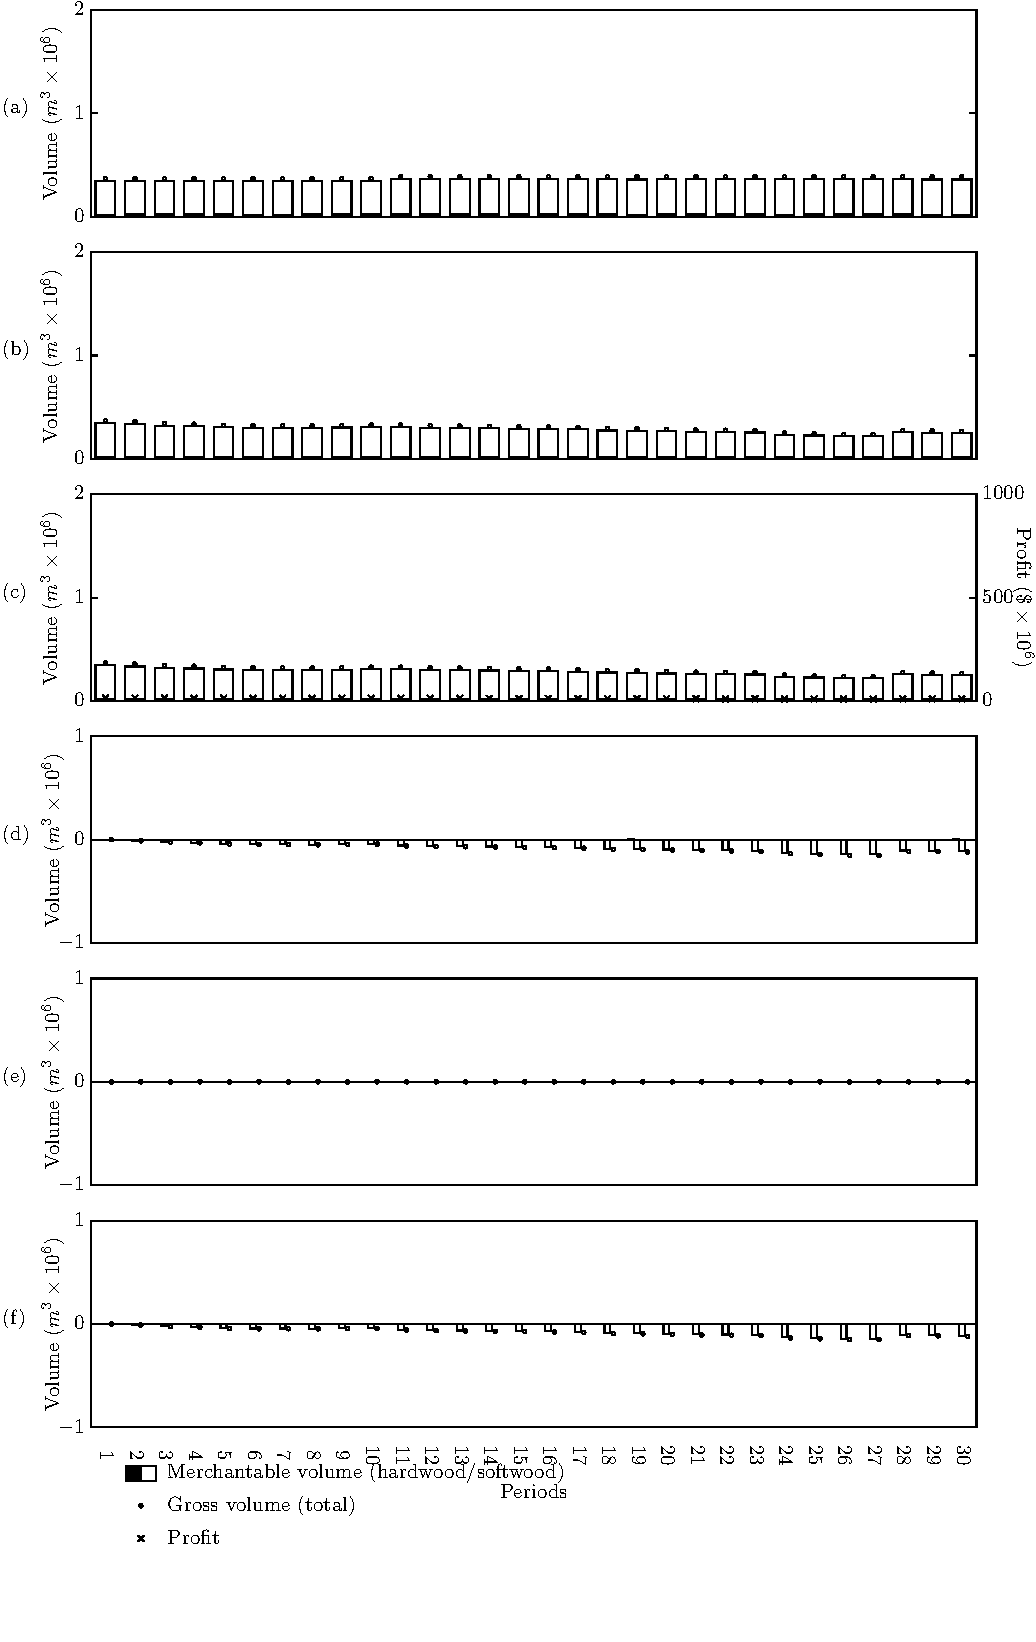
\includegraphics[width=10cm]{images/appendix/s6-2x_test00}
  \caption{Scenario 6-2x\_f1.0}
  \label{fig:s6-2x_test00}
\end{figure}

\begin{figure}[h]
  \centering
  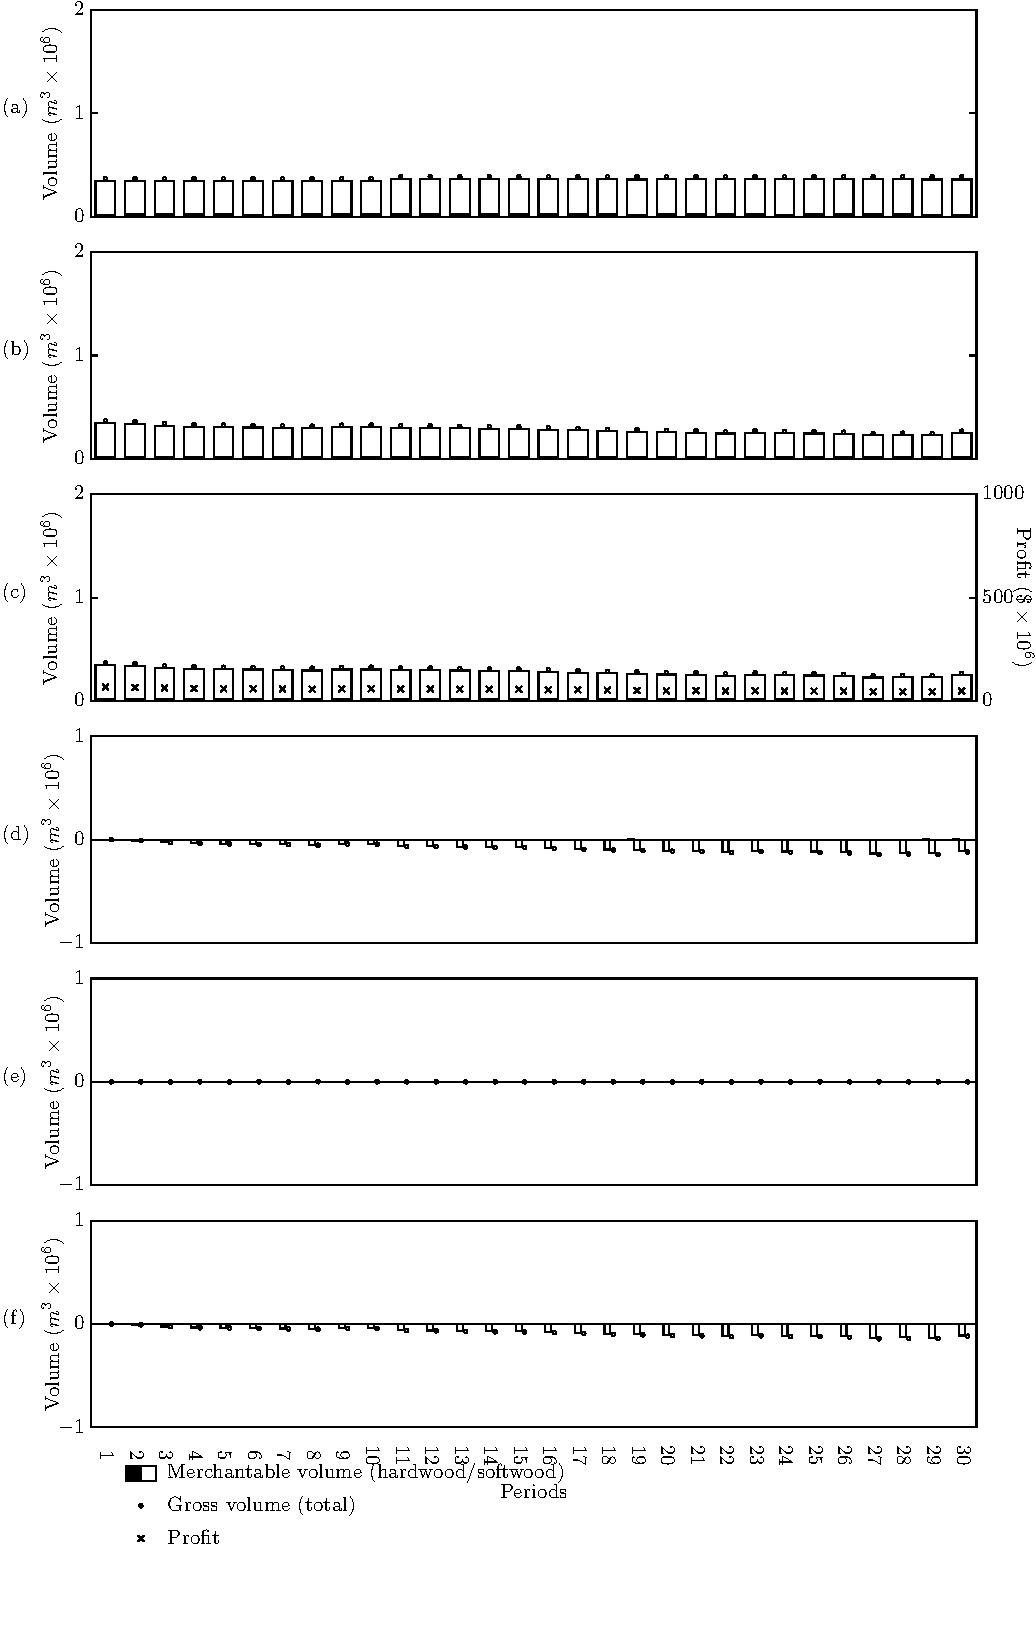
\includegraphics[width=10cm]{images/appendix/s6-2x_test10}
  \caption{Scenario 6-2x\_f1.6}
  \label{fig:s6-2x_test10}
\end{figure}

\begin{figure}[h]
  \centering
  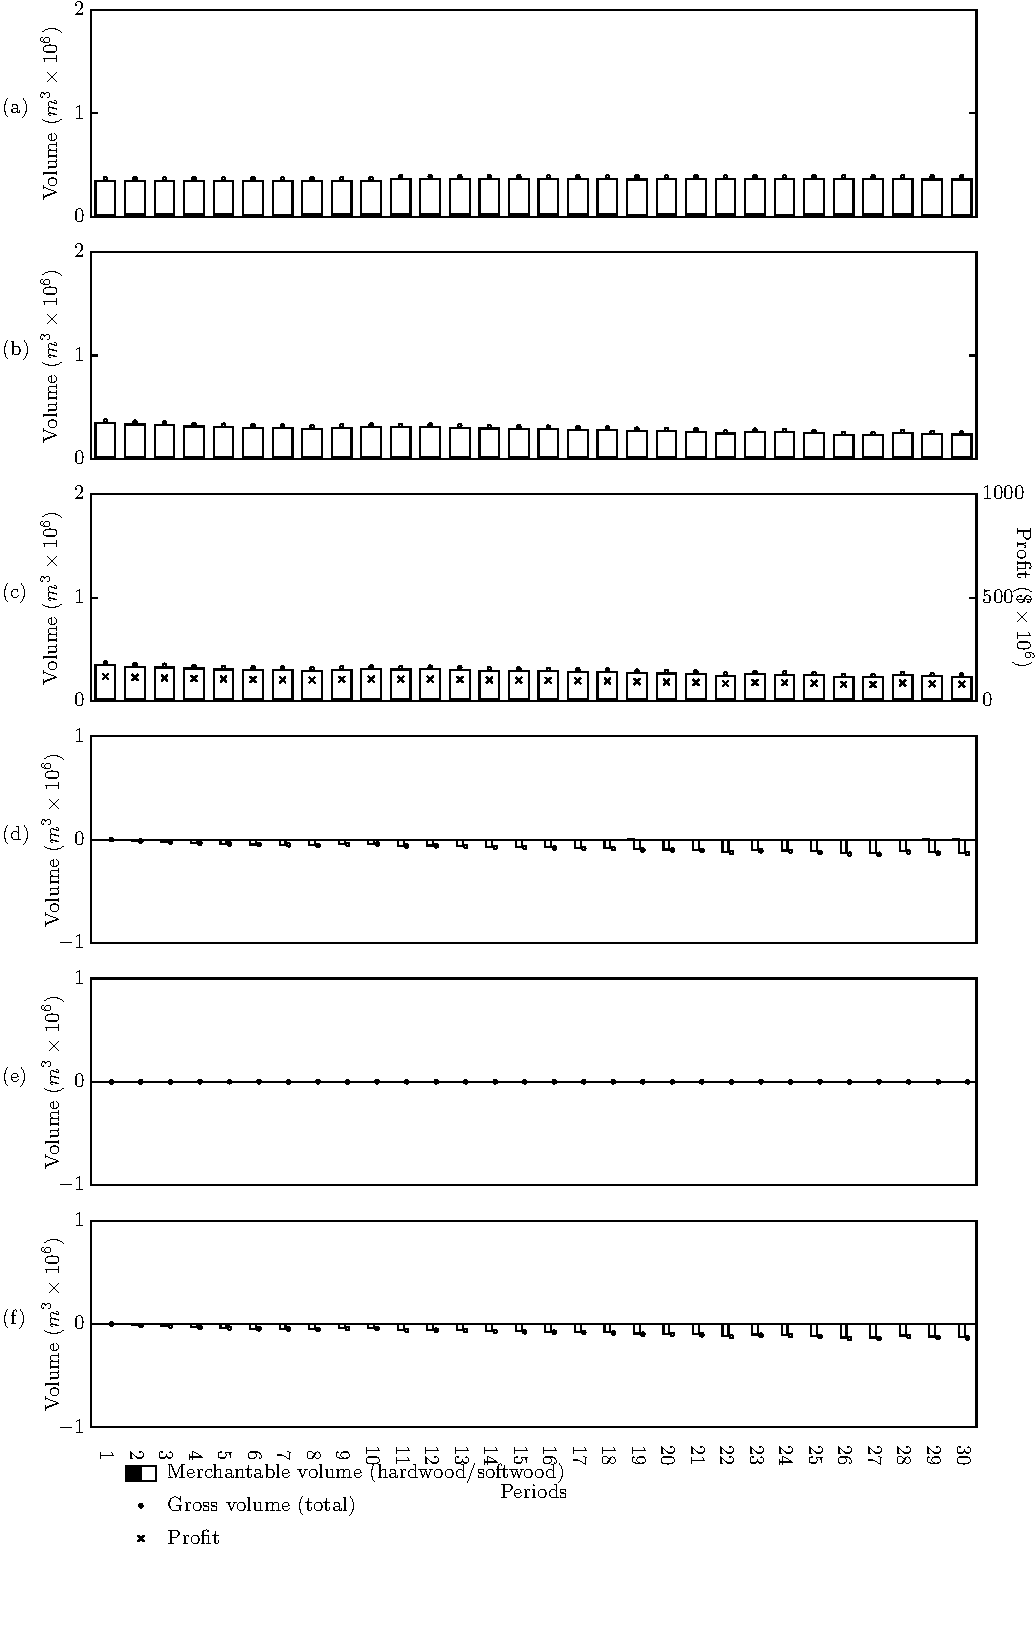
\includegraphics[width=10cm]{images/appendix/s6-2x_test20}
  \caption{Scenario 6-2x\_f2.2}
  \label{fig:s6-2x_test20}
\end{figure}

\begin{figure}[h]
  \centering
  \includegraphics[width=10cm]{images/appendix/s6-2x_test30}
  \caption{Scenario 6-2x\_f2.8}
  \label{fig:s6-2x_test30}
\end{figure}

\begin{figure}[h]
  \centering
  \includegraphics[width=10cm]{images/appendix/s6-2x_test40}
  \caption{Scenario 6-2x\_f3.4}
  \label{fig:s6-2x_test40}
\end{figure}

\begin{figure}[h]
  \centering
  \includegraphics[width=10cm]{images/appendix/s6-2x_test50}
  \caption{Scenario 6-2x\_f4.0}
  \label{fig:s6-2x_test50}
\end{figure}

\begin{figure}[h]
  \centering
  \includegraphics[width=10cm]{images/appendix/s6-2x_test60}
  \caption{Scenario 6-2x\_f4.6}
  \label{fig:s6-2x_test60}
\end{figure}

\begin{figure}[h]
  \centering
  \includegraphics[width=10cm]{images/appendix/s6-2x_test70}
  \caption{Scenario 6-2x\_f5.3}
  \label{fig:s6-2x_test70}
\end{figure}

\begin{figure}[h]
  \centering
  \includegraphics[width=10cm]{images/appendix/s6-2x_test80}
  \caption{Scenario 6-2x\_f5.9}
  \label{fig:s6-2x_test80}
\end{figure}

\begin{figure}[h]
  \centering
  \includegraphics[width=10cm]{images/appendix/s6-2x_test90}
  \caption{Scenario 6-2x\_f6.4}
  \label{fig:s6-2x_test90}
\end{figure}

\begin{figure}[h]
  \centering
  \includegraphics[width=10cm]{images/appendix/s6-2x_test100}
  \caption{Scenario 6-2x\_f7.1}
  \label{fig:s6-2x_test100}
\end{figure}
   
%\chapter{Scenario Series 6-2y}

This appendix presents simulation results from the 6-2y scenario series, which tests the impact of decreasing end-product prices in the agent network. 
We decrease all products prices proportionately (i.e., perfectly correlated price increase, relative to base values), and keep them constant for all 30 iterations. 

\section{Summary}
Table \ref{tab:scenario_list} below lists the scenarios in series 6-2x.
 
Base scenario s6-2x\_f1.0 is identical to s6-1\_p30a01, and simulates a basic bilevel scenario with default prices (i.e., scaling factor 1.0).
We tested scaling factors of 0.90 and 0.85. 
Profit is reduced significantly in the 0.90 scenario, however harvest levels are minimally impacted.
Hardwood price drops below the break-even point for the 0.85 scenario, which causes upper bound on the hardwood log consumption in the bilevel algorithm to drop suddenly to 0. 
This implies that agent softwood procurement must be limited to true pure softwood stands (i.e., absolutely no hardwood content in the yield curve model at harvest age). 
True pure softwood stands are quite rare in our dataset, so softwood log consumption drops to a very low level (approximately 1\% of base scenario fibre consumption).
Simulation results for scenarios testing factors less than 0.85 were omitted, as harvest drops to 0 for both hardwood and softwood.

\begin{table}
  \centering
  \begin{tabular}{lll}
    \hline
    Scenario ID & Figure Reference & Description \\
    \hline
    6-2y\_f1.00 & \ref{fig:s6-2y_test100} & Control scenario (same as s6-1\_p30a01). \\
    6-2y\_f0.90 & \ref{fig:s6-2y_test090} & Prices scaled by factor of 0.90 \\
    6-2y\_f0.85 & \ref{fig:s6-2y_test085} & Prices scaled by factor of 0.85 \\
    % 6-2y\_f5.3 & \ref{fig:s6-2y_test70} & Prices scaled by factor of 0.7 \\
    % 6-2y\_f4.6 & \ref{fig:s6-2y_test60} & Prices scaled by factor of 0.6 \\
    % 6-2y\_f4.0 & \ref{fig:s6-2y_test50} & Prices scaled by factor of 0.5 \\
    % 6-2y\_f3.4 & \ref{fig:s6-2y_test40} & Prices scaled by factor of 0.4 \\
    % 6-2y\_f2.8 & \ref{fig:s6-2y_test30} & Prices scaled by factor of 0.3 \\
    % 6-2y\_f2.2 & \ref{fig:s6-2y_test20} & Prices scaled by factor of 0.2 \\
    % 6-2y\_f1.6 & \ref{fig:s6-2y_test10} & Prices scaled by factor of 0.1 \\
    \hline
  \end{tabular}
  \caption{Description of scenarios in series 6-2y.}
  \label{tab:scenario_list}
\end{table}


\section{Results}

Figures \ref{fig:s6-2y_test100} to \ref{fig:s6-2y_test085} present
simulation results for fifteen scenarios. % Table \ref{tab:scenarios}
% summarizes scenario parameters used in the experiment for each
% scenario.
Disposition of figures is identical for all scenarios. The
first subfigure (a) for each scenario shows the initial
(ie. iteration-0) AAC solution. The second subfigure (b) for each
scenario shows first period of AAC solution for all 30 planning
iterations. The third subfigure (c) for each scenario shows the
implemented harvest level for all 30 planning iterations. Scenarios
3.1 and 3.2 also show profit in this subfigure on a secondary
axis. The fourth subfigure (d) for each scenario shows the difference
between initial and re-planned AAC. The fifth subfigure (e) for each
scenario shows the difference between re-planned AAC and harvest.  The
sixth subfigure (f) for each scenario shows the difference between
initial AAC and harvest. Softwood volume is shown with white bars,
hardwood volume with black bars, and total volume with small
circles. Profit (where applicable) is shown with the $\times$
symbol. 

\begin{figure}[h]
  \centering
  \includegraphics[width=10cm]{images/appendix/s6-1_p30a01}
  \caption{Scenario 6-2y\_f1.0}
  \label{fig:s6-2y_test100}
\end{figure}


\begin{figure}[h]
  \centering
  \includegraphics[width=10cm]{images/appendix/s6-2y_test090}
  \caption{Scenario 6-2y\_f6.4}
  \label{fig:s6-2y_test090}
\end{figure}

\begin{figure}[h]
  \centering
  \includegraphics[width=10cm]{images/appendix/s6-2y_test085}
  \caption{Scenario 6-2y\_f0.85}
  \label{fig:s6-2y_test085}
\end{figure}

% \begin{figure}[h]
%   \centering
%   \includegraphics[width=10cm]{images/appendix/s6-2y_test70}
%   \caption{Scenario 6-2y\_f5.3}
%   \label{fig:s6-2y_test70}
% \end{figure}

% \begin{figure}[h]
%   \centering
%   \includegraphics[width=10cm]{images/appendix/s6-2y_test50}
%   \caption{Scenario 6-2y\_f4.0}
%   \label{fig:s6-2y_test50}
% \end{figure}

% \begin{figure}[h]
%   \centering
%   \includegraphics[width=10cm]{images/appendix/s6-2y_test40}
%   \caption{Scenario 6-2y\_f3.4}
%   \label{fig:s6-2y_test40}
% \end{figure}

% \begin{figure}[h]
%   \centering
%   \includegraphics[width=10cm]{images/appendix/s6-2y_test30}
%   \caption{Scenario 6-2y\_f2.8}
%   \label{fig:s6-2y_test30}
% \end{figure}

% \begin{figure}[h]
%   \centering
%   \includegraphics[width=10cm]{images/appendix/s6-2y_test20}
%   \caption{Scenario 6-2y\_f2.2}
%   \label{fig:s6-2y_test20}
% \end{figure}

% \begin{figure}[h]
%   \centering
%   \includegraphics[width=10cm]{images/appendix/s6-2y_test10}
%   \caption{Scenario 6-2y\_f1.6}
%   \label{fig:s6-2y_test10}
% \end{figure}
   
%\chapter{Scenario Series 6-4}

This appendix presents simulation results from the 6-4 scenario series, this tests impact of varying softwood AAC attribution level. 

\section{Summary}
Table \ref{tab:scenario_list} below lists the scenarios in series 6-4. 
Control scenario s6-0 simulates the \emph{status quo} situation (single-level wood supply model with no anticipation of fibre consumption).  

\begin{table}
  \centering
  \begin{tabular}{lll}
    \hline
    Scenario ID & Figure Reference & Description \\
    \hline
    6-0 & \ref{fig:s6-0} & Control scenario. \\
    6-4\_hw100sw110 & \ref{fig:s6-4_hw100sw110} & 110$\%$ of softwood AAC allocated. \\
    6-4\_hw100sw105 & \ref{fig:s6-4_hw100sw105} & 105\% of softwood AAC allocated. \\
    6-4\_hw100sw100 & \ref{fig:s6-4_hw100sw095} & 100$\%$ of softwood AAC allocated\footnote{Identical to scenario 6-1\_p30a01.}. \\
    6-4\_hw100sw095 & \ref{fig:s6-4_hw100sw095} & 95$\%$ of softwood AAC allocated. \\
    6-4\_hw100sw090 & \ref{fig:s6-4_hw100sw090} & 90\% of softwood AAC allocated. \\
    6-4\_hw100sw080 & \ref{fig:s6-4_hw100sw080} & 80\% of softwood AAC allocated. \\
    6-4\_hw100sw060 & \ref{fig:s6-4_hw100sw060} & 60\% of softwood AAC allocated. \\
    \hline
  \end{tabular}
  \caption{Description of scenarios in series 6-4.}
  \label{tab:scenario_list}
\end{table}

\section{Results}

Figures \ref{fig:s6-4_hw100sw100} to \ref{fig:s6-4_hw100sw060} present
simulation results for fifteen scenarios. % Table \ref{tab:scenarios}
% summarizes scenario parameters used in the experiment for each
% scenario.
Disposition of figures is identical for all scenarios. The
first subfigure (a) for each scenario shows the initial
(ie. iteration-0) AAC solution. The second subfigure (b) for each
scenario shows first period of AAC solution for all 30 planning
iterations. The third subfigure (c) for each scenario shows the
implemented harvest level for all 30 planning iterations. Scenarios
3.1 and 3.2 also show profit in this subfigure on a secondary
axis. The fourth subfigure (d) for each scenario shows the difference
between initial and re-planned AAC. The fifth subfigure (e) for each
scenario shows the difference between re-planned AAC and harvest.  The
sixth subfigure (f) for each scenario shows the difference between
initial AAC and harvest. Softwood volume is shown with white bars,
hardwood volume with black bars, and total volume with small
circles. Profit (where applicable) is shown with the $\times$
symbol. 

Hardwood AAC attribution level is kept constant at 100\% for all scenarios. 
As might be expected, softwood attribution levels above 100\% of AAC show more variability in harvest levels and profit, compared to lower-attribution scenarios.
However, impact of over-attributing softwood is relatively low. This may be due to limited availability of pure softwood stands, forcing agent to harvest mixed stands, which in turn saturates the hardwood line.

We can observe declining profit and AAC at, and well below, 100\% softwood AAC attribution level. 
In fact, softwood attribution must be limited to 60\% of AAC to stabilise harvest level and profit over all 30 rolling-horizon replanning cycles.


\begin{figure}[h]
  \centering
  \includegraphics[width=10cm]{images/appendix/s6-0}
  \caption{Scenario 6-0 (control scenario, simulates \emph{status quo}).}
  \label{fig:s6-0}
\end{figure}


\begin{figure}[h]
  \centering
  \includegraphics[width=10cm]{images/appendix/s6-4_hw100sw110}
  \caption{Scenario 6-4\_hw100sw110 (110\% of softwood AAC allocated).}
  \label{fig:s6-4_hw100sw110}
\end{figure}

\begin{figure}[h]
  \centering
  \includegraphics[width=10cm]{images/appendix/s6-4_hw100sw105}
  \caption{Scenario 6-4\_hw100sw105 (105\% of softwood AAC allocated).}
  \label{fig:s6-4_hw100sw105}
\end{figure}

\begin{figure}[h]
  \centering
  \includegraphics[width=10cm]{images/appendix/s6-1_p30a01}
  \caption{Scenario 6-4\_hw100sw100 (100\% of softwood AAC allocated).}
  \label{fig:s6-4_hw100sw100}
\end{figure}

\begin{figure}[h]
  \centering
  \includegraphics[width=10cm]{images/appendix/s6-4_hw100sw095}
  \caption{Scenario 6-4\_hw100sw095 (95\% of softwood AAC allocated).}
  \label{fig:s6-4_hw100sw095}
\end{figure}

\begin{figure}[h]
  \centering
  \includegraphics[width=10cm]{images/appendix/s6-4_hw100sw090}
  \caption{Scenario 6-4\_hw100sw090 (90\% of softwood AAC allocated).}
  \label{fig:s6-4_hw100sw090}
\end{figure}

\begin{figure}[h]
  \centering
  \includegraphics[width=10cm]{images/appendix/s6-4_hw100sw080}
  \caption{Scenario 6-4\_hw100sw080 (80\% of softwood AAC allocated).}
  \label{fig:s6-4_hw100sw080}
\end{figure}

\begin{figure}[h]
  \centering
  \includegraphics[width=10cm]{images/appendix/s6-4_hw100sw060}
  \caption{Scenario 6-4\_hw100sw060 (60\% of softwood AAC allocated).}
  \label{fig:s6-4_hw100sw060}
\end{figure}
   
%\chapter{Scenario Series 6-5}

This appendix presents simulation results from the 6-5 scenario series, this tests impact of varying tightness of even flow constraints for hardwood and softwood AAC. 

\section{Summary}
Table \ref{tab:scenario_list} below lists the scenarios in this series. 

This scenario series tests impact of varying slack in of species-wise even-flow constraints in the principal's wood supply model. 
The default slack for all other scenario series is 5\% (i.e., periodic harvest volume must be within interval $(0.95 v_{max}, 1.00 v_{max})$, where $v_{max}$ represents the maximum periodic harvest volume for a given solution). 

Increasing even-flow constraint slack seems to have a moderate negative impact on stability of harvest levels and profit. This is not entirely surprising, if one considers that the principal's wood supply plans are optimal solutions to deterministic problems, and that adding slack to the even-flow constraint produces more and more jagged (deterministic) harvest profiles. Any deviation, however small, from the optimal solution will either produce an alternative optimal solution (unlikely), a suboptimal feasible solution, or an infeasible solution. We know there are deviations in the base case (with 5\% slack), and we know this causes some measurable drift over time. Adding more variability to the optimal solutions is not likely to reduce these deviations on average.

Also, the even-flow constraints are defined \emph{species-wise}, which means that softwood harvest level might jump up in the first period while hardwood harvest jumps down. In this example, the agent would have to include a greater-than-usual proportion of pure softwood stands in his harvest plan to satisfy softwood demand while harvesting an unusually-low hardwood volume. This would tend to aggravate the existing high-grading problem, which is responsible for residual drift.

Overall, the best scenario in this series (in terms of stability, harvest level, and profit) is scenario 6-5\_hw000sw000 (i.e., perfectly tight even-flow constraints).

\begin{table}
  \centering
  \begin{tabular}{lll}
    \hline
    Scenario ID & Figure Reference & Description \\
    \hline
    3-1 & \ref{fig:s3-1} & Control (\emph{status quo}). \\
    6-5\_hw005sw005 & \ref{fig:s6-5_hw005sw005} & Hardwood: 0\%, softwood: 0\%. \\
    6-5\_hw005sw005 & \ref{fig:s6-5_hw005sw005} & Hardwood: 1\%, softwood: 1\%. \\
    6-5\_hw005sw005 & \ref{fig:s6-5_hw005sw005} & Hardwood: 5\%, softwood: 5\%. \\
    6-4\_hw099sw005 & \ref{fig:s6-5_hw099sw005} & Hardwood: 99\%, softwood: 5\%. \\
    6-4\_hw010sw010 & \ref{fig:s6-5_hw010sw010} & Hardwood: 10\%, softwood: 10\%. \\
    6-4\_hw020sw020 & \ref{fig:s6-5_hw020sw020} & Hardwood: 20\%, softwood: 20\%. \\
    6-4\_hw050sw050 & \ref{fig:s6-5_hw050sw050} & Hardwood: 50\%, softwood: 50\%. \\

    \hline
  \end{tabular}
  \caption{Description of scenarios in series 6-5.}
  \label{tab:scenario_list}
\end{table}

\section{Results}

Figures \ref{fig:s6-5_hw005sw005} to \ref{fig:s6-5_hw050sw050} present
simulation results for fifteen scenarios. % Table \ref{tab:scenarios}
% summarizes scenario parameters used in the experiment for each
% scenario.
Disposition of figures is identical for all scenarios. The
first subfigure (a) for each scenario shows the initial
(ie. iteration-0) AAC solution. The second subfigure (b) for each
scenario shows first period of AAC solution for all 30 planning
iterations. The third subfigure (c) for each scenario shows the
implemented harvest level for all 30 planning iterations. Scenarios
3.1 and 3.2 also show profit in this subfigure on a secondary
axis. The fourth subfigure (d) for each scenario shows the difference
between initial and re-planned AAC. The fifth subfigure (e) for each
scenario shows the difference between re-planned AAC and harvest.  The
sixth subfigure (f) for each scenario shows the difference between
initial AAC and harvest. Softwood volume is shown with white bars,
hardwood volume with black bars, and total volume with small
circles. Profit (where applicable) is shown with the $\times$
symbol. 


\begin{figure}[h]
  \centering
  \includegraphics[width=10cm]{images/appendix/s3-1}
  \caption{Scenario 3-1 (\emph{status quo}).}
  \label{fig:s3-1}
\end{figure}

\begin{figure}[h]
  \centering
  \includegraphics[width=10cm]{images/appendix/s6-5_hw000sw000}
  \caption{Scenario 6-5\_hw000sw000 (hardwood: 0\%, softwood: 0\%).}
  \label{fig:s6-5_hw000sw000}
\end{figure}

\begin{figure}[h]
  \centering
  \includegraphics[width=10cm]{images/appendix/s6-5_hw001sw001}
  \caption{Scenario 6-5\_hw001sw001 (hardwood: 1\%, softwood: 1\%).}
  \label{fig:s6-5_hw001sw001}
\end{figure}

\begin{figure}[h]
  \centering
  \includegraphics[width=10cm]{images/appendix/s6-1_p30a01}
  \caption{Scenario 6-5\_hw005sw005 (hardwood: 5\%, softwood: 5\%).}
  \label{fig:s6-5_hw005sw005}
\end{figure}


\begin{figure}[h]
  \centering
  \includegraphics[width=10cm]{images/appendix/s6-5_hw099sw005}
  \caption{Scenario 6-5\_hw099sw005 (hardwood: 99\%, softwood: 5\%).}
  \label{fig:s6-5_hw099sw005}
\end{figure}

\begin{figure}[h]
  \centering
  \includegraphics[width=10cm]{images/appendix/s6-5_hw010sw010}
  \caption{Scenario 6-5\_hw010sw010 (hardwood: 10\%, softwood: 10\%).}
  \label{fig:s6-5_hw010sw010}
\end{figure}

\begin{figure}[h]
  \centering
  \includegraphics[width=10cm]{images/appendix/s6-5_hw020sw020}
  \caption{Scenario 6-5\_hw020sw020 (hardwood: 20\%, softwood: 20\%).}
  \label{fig:s6-5_hw020sw020}
\end{figure}

\begin{figure}[h]
  \centering
  \includegraphics[width=10cm]{images/appendix/s6-5_hw050sw050}
  \caption{Scenario 6-5\_hw050sw050 (hardwood: 50\%, softwood: 50\%).}
  \label{fig:s6-5_hw050sw050}
\end{figure}

%\chapter{Scenario Series 6-6}

This document presents simulation results from the 6-6 scenario series, which tests impact of relaxing line-wise agent profitability constraint (both in bilevel anticipation, and in simulated agent behaviour). 
This simulates perfectly integrated (i.e., collaborative) agent fibre procurement behaviour, and makes it possible for the hardwood line to operate at a net loss if this is profitable for the network as a whole. 
This is a hypothetical scenario, as it makes optimistic assumptions regarding willingness of the hardwood line to operate at a net loss to benefit the rest of the network.
Some form of collaborative benefit-sharing agreement would have to been in place for this setup to be economically viable for the hardwood sub-agent, however no such agreements are in place in reality.

\section{Summary}
Table \ref{tab:scenario_list} below lists the scenarios in series 6-6. 

\begin{table}
  \centering
  \begin{tabular}{lll}
    \hline
    Scenario ID & Figure Reference & Description \\
    \hline
    6-6\_base & \ref{fig:s6-6_base} & Base scenario. \\
    \hline
  \end{tabular}
  \caption{Description of scenarios in series 6-6.}
  \label{tab:scenario_list}
\end{table}

\section{Results}

Figure \ref{fig:s6-6_base} presents
simulation results for fifteen scenarios. % Table \ref{tab:scenarios}
% summarizes scenario parameters used in the experiment for each
% scenario.
Disposition of figures is identical for all scenarios. The
first subfigure (a) for each scenario shows the initial
(ie. iteration-0) AAC solution. The second subfigure (b) for each
scenario shows first period of AAC solution for all 30 planning
iterations. The third subfigure (c) for each scenario shows the
implemented harvest level for all 30 planning iterations. Scenarios
3.1 and 3.2 also show profit in this subfigure on a secondary
axis. The fourth subfigure (d) for each scenario shows the difference
between initial and re-planned AAC. The fifth subfigure (e) for each
scenario shows the difference between re-planned AAC and harvest.  The
sixth subfigure (f) for each scenario shows the difference between
initial AAC and harvest. Softwood volume is shown with white bars,
hardwood volume with black bars, and total volume with small
circles. Profit (where applicable) is shown with the $\times$
symbol. 

\begin{figure}[h]
  \centering
  \includegraphics[width=10cm]{images/appendix/s6-6_base}
  \caption{Scenario 6-6\_base (base scenario).}
  \label{fig:s6-6_base}
\end{figure}

   
%\include{appendix_scenario-series_6-7}   % stochastic demand scenario... document not compiled yet
   

\bibliographystyle{plainnat}
\bibliography{phd}  

\end{document}
